\section{Code}

All code used is published at \url{https://github.com/samuel-book/samuel-3}

\subsection{Python packages used}

The following packages were used for the analysis:

\begin{itemize}
    \item Python 3.12.13 \url{https://www.python.org/}
    \item Pandas 3.0.3 \url{https://pandas.pydata.org/}
    \item MatPlotLib 3.11.0 \url{https://matplotlib.org/}
    \item Seaborn 0.13.2 \url{https://seaborn.pydata.org/}
    \item XGBoost 2.1.4 \url{https://xgboost.ai/}
    \item LightGBM 4.6.0 \url{https://lightgbm.readthedocs.io/}
    \item EconML 0.16.0 \url{https://www.pywhy.org/EconML/}
    \item SHAP 0.48.0 \url{https://shap.readthedocs.io/}
    \item Statsmodels 0.14.6 \url{https://www.statsmodels.org/}
    \item SciKit-Learn 1.6.1 \url{https://scikit-learn.org} 
\end{itemize}

\section{Data}

\begin{landscape}
\subsection{Descriptive statistics}


{
\footnotesize
\begin{longtable}[]{@{}llllllllll@{}}
% Header on first page
\caption{Descriptive statistics for each reperfusion treatment group. Strategies are defined by early ($\leq$ 270 mins from onset) or late ($>$ 270 mins from onset) intravenous thrombolysis, mechanical thrombectomy, or their combination.}
\label{tab:full_group_stats}\\
\toprule
Feature & Statistic & No treatment & Early IVT only & Late IVT only &
Early MT only & Late MT only & Early IVT/MT & Early IVT + Late
MT & Late IVT/MT \\
\midrule
\endfirsthead
% Headers on subsequent pages
\caption[]{\tablename~\thetable{} continued}\\
\toprule
Feature & Statistic & No treatment & Early IVT only & Late IVT only &
Early MT only & Late MT only & Early IVT/MT & Early IVT + Late
MT & Late IVT/MT \\
\midrule
\endhead

\bottomrule
\endlastfoot
Prior disability & count & 30,914 & 23,074 & 973 & 1,207 & 526 & 2,570 &
226 & 80 \\
& mean & 1.84 & 0.98 & 0.98 & 0.64 & 0.53 & 0.36 & 0.45 & 0.50 \\
& std & 1.60 & 1.31 & 1.31 & 0.82 & 0.84 & 0.69 & 0.79 & 0.76 \\
& min & 0.00 & 0.00 & 0.00 & 0.00 & 0.00 & 0.00 & 0.00 & 0.00 \\
& 25\% & 0.00 & 0.00 & 0.00 & 0.00 & 0.00 & 0.00 & 0.00 & 0.00 \\
& 50\% & 2.00 & 0.00 & 0.00 & 0.00 & 0.00 & 0.00 & 0.00 & 0.00 \\
& 75\% & 3.00 & 2.00 & 2.00 & 1.00 & 1.00 & 1.00 & 1.00 & 1.00 \\
& max & 5.00 & 5.00 & 5.00 & 4.00 & 5.00 & 5.00 & 4.00 & 3.00 \\
\midrule
Stroke severity & count & 30,877 & 23,058 & 973 & 1,206 & 526 & 2,570 &
226 & 80 \\
& mean & 12.87 & 12.73 & 12.00 & 16.61 & 14.93 & 16.29 & 14.70 &
14.35 \\
& std & 6.75 & 6.18 & 5.99 & 5.89 & 6.53 & 6.00 & 6.26 & 5.53 \\
& min & 0.00 & 0.00 & 0.00 & 0.00 & 1.00 & 0.00 & 2.00 & 6.00 \\
& 25\% & 7.00 & 8.00 & 7.00 & 12.00 & 10.00 & 12.00 & 10.00 & 9.75 \\
& 50\% & 11.00 & 11.00 & 10.00 & 17.00 & 14.50 & 17.00 & 14.50 &
14.00 \\
& 75\% & 17.00 & 17.00 & 16.00 & 21.00 & 20.00 & 21.00 & 19.00 &
18.25 \\
& max & 42.00 & 42.00 & 35.00 & 40.00 & 37.00 & 37.00 & 35.00 & 28.00 \\
\midrule
Age & count & 30,914 & 23,074 & 973 & 1,207 & 526 & 2,570 & 226 & 80 \\
& mean & 78.51 & 74.23 & 74.05 & 74.00 & 71.83 & 71.08 & 67.61 &
71.62 \\
& std & 12.36 & 13.29 & 13.21 & 12.60 & 13.45 & 12.97 & 14.26 & 14.09 \\
& min & 37.50 & 37.50 & 37.50 & 37.50 & 37.50 & 37.50 & 37.50 & 37.50 \\
& 25\% & 72.50 & 67.50 & 67.50 & 67.50 & 62.50 & 62.50 & 57.50 &
62.50 \\
& 50\% & 82.50 & 77.50 & 77.50 & 77.50 & 77.50 & 72.50 & 72.50 &
77.50 \\
& 75\% & 87.50 & 82.50 & 82.50 & 82.50 & 82.50 & 82.50 & 77.50 &
82.50 \\
& max & 92.50 & 92.50 & 92.50 & 92.50 & 92.50 & 92.50 & 92.50 & 92.50 \\
\midrule
Congestive heart failure & count & 30,914 & 23,074 & 973 & 1,207 & 526 &
2,570 & 226 & 80 \\
& mean & 0.09 & 0.05 & 0.05 & 0.09 & 0.06 & 0.04 & 0.05 & 0.09 \\
& std & 0.29 & 0.22 & 0.23 & 0.29 & 0.25 & 0.19 & 0.22 & 0.28 \\
& min & 0.00 & 0.00 & 0.00 & 0.00 & 0.00 & 0.00 & 0.00 & 0.00 \\
& 25\% & 0.00 & 0.00 & 0.00 & 0.00 & 0.00 & 0.00 & 0.00 & 0.00 \\
& 50\% & 0.00 & 0.00 & 0.00 & 0.00 & 0.00 & 0.00 & 0.00 & 0.00 \\
& 75\% & 0.00 & 0.00 & 0.00 & 0.00 & 0.00 & 0.00 & 0.00 & 0.00 \\
& max & 1.00 & 1.00 & 1.00 & 1.00 & 1.00 & 1.00 & 1.00 & 1.00 \\
\midrule
Hypertension & count & 30,914 & 23,074 & 973 & 1,207 & 526 & 2,570 & 226
& 80 \\
& mean & 0.59 & 0.55 & 0.57 & 0.56 & 0.52 & 0.51 & 0.43 & 0.48 \\
& std & 0.49 & 0.50 & 0.50 & 0.50 & 0.50 & 0.50 & 0.50 & 0.50 \\
& min & 0.00 & 0.00 & 0.00 & 0.00 & 0.00 & 0.00 & 0.00 & 0.00 \\
& 25\% & 0.00 & 0.00 & 0.00 & 0.00 & 0.00 & 0.00 & 0.00 & 0.00 \\
& 50\% & 1.00 & 1.00 & 1.00 & 1.00 & 1.00 & 1.00 & 0.00 & 0.00 \\
& 75\% & 1.00 & 1.00 & 1.00 & 1.00 & 1.00 & 1.00 & 1.00 & 1.00 \\
& max & 1.00 & 1.00 & 1.00 & 1.00 & 1.00 & 1.00 & 1.00 & 1.00 \\
\midrule
Diabetes & count & 30,914 & 23,074 & 973 & 1,207 & 526 & 2,570 & 226 &
80 \\
& mean & 0.26 & 0.21 & 0.24 & 0.19 & 0.17 & 0.15 & 0.18 & 0.24 \\
& std & 0.44 & 0.41 & 0.43 & 0.39 & 0.38 & 0.36 & 0.38 & 0.43 \\
& min & 0.00 & 0.00 & 0.00 & 0.00 & 0.00 & 0.00 & 0.00 & 0.00 \\
& 25\% & 0.00 & 0.00 & 0.00 & 0.00 & 0.00 & 0.00 & 0.00 & 0.00 \\
& 50\% & 0.00 & 0.00 & 0.00 & 0.00 & 0.00 & 0.00 & 0.00 & 0.00 \\
& 75\% & 1.00 & 0.00 & 0.00 & 0.00 & 0.00 & 0.00 & 0.00 & 0.00 \\
& max & 1.00 & 1.00 & 1.00 & 1.00 & 1.00 & 1.00 & 1.00 & 1.00 \\
\midrule
Afib anticoagulant & count & 30,914 & 23,074 & 973 & 1,207 & 526 & 2,570
& 226 & 80 \\
& mean & 0.29 & 0.03 & 0.03 & 0.56 & 0.24 & 0.03 & 0.04 & 0.05 \\
& std & 0.45 & 0.18 & 0.18 & 0.50 & 0.43 & 0.17 & 0.19 & 0.22 \\
& min & 0.00 & 0.00 & 0.00 & 0.00 & 0.00 & 0.00 & 0.00 & 0.00 \\
& 25\% & 0.00 & 0.00 & 0.00 & 0.00 & 0.00 & 0.00 & 0.00 & 0.00 \\
& 50\% & 0.00 & 0.00 & 0.00 & 1.00 & 0.00 & 0.00 & 0.00 & 0.00 \\
& 75\% & 1.00 & 0.00 & 0.00 & 1.00 & 0.00 & 0.00 & 0.00 & 0.00 \\
& max & 1.00 & 1.00 & 1.00 & 1.00 & 1.00 & 1.00 & 1.00 & 1.00 \\
\midrule
Afib diagnosis & count & 30,914 & 23,074 & 973 & 1,207 & 526 & 2,570 &
226 & 80 \\
& mean & 0.39 & 0.21 & 0.20 & 0.58 & 0.37 & 0.25 & 0.21 & 0.25 \\
& std & 0.49 & 0.41 & 0.40 & 0.49 & 0.48 & 0.43 & 0.41 & 0.44 \\
& min & 0.00 & 0.00 & 0.00 & 0.00 & 0.00 & 0.00 & 0.00 & 0.00 \\
& 25\% & 0.00 & 0.00 & 0.00 & 0.00 & 0.00 & 0.00 & 0.00 & 0.00 \\
& 50\% & 0.00 & 0.00 & 0.00 & 1.00 & 0.00 & 0.00 & 0.00 & 0.00 \\
& 75\% & 1.00 & 0.00 & 0.00 & 1.00 & 1.00 & 0.00 & 0.00 & 0.25 \\
& max & 1.00 & 1.00 & 1.00 & 1.00 & 1.00 & 1.00 & 1.00 & 1.00 \\
\midrule
Onset to thrombolysis & count & NA & 23,074 & 973 & NA & NA & 2,570
& 226 & 80 \\
& mean & NA & 163.81 & 298.36 & NA & NA & 142.54 & 209.79 & 305.81 \\
& std & NA & 50.38 & 23.58 & NA & NA & 45.57 & 50.11 & 25.13 \\
& min & NA & 14.00 & 271.00 & NA & NA & 22.00 & 71.00 & 271.00 \\
& 25\% & NA & 125.00 & 279.00 & NA & NA & 109.00 & 177.25 & 281.75 \\
& 50\% & NA & 160.00 & 291.00 & NA & NA & 136.00 & 224.00 & 301.00 \\
& 75\% & NA & 200.00 & 314.00 & NA & NA & 175.00 & 254.75 & 327.00 \\
& max & NA & 270.00 & 359.00 & NA & NA & 265.00 & 270.00 & 358.00 \\
\midrule
Onset to thrombectomy & count & NA & NA & NA & 1,207 & 526 & 2,570
& 226 & 80 \\
& mean & NA & NA & NA & 163.20 & 385.55 & 163.43 & 365.01 & 333.44 \\
& std & NA & NA & NA & 53.56 & 100.30 & 48.88 & 123.99 & 55.31 \\
& min & NA & NA & NA & 0.00 & 270.00 & 38.00 & 270.00 & 276.00 \\
& 25\% & NA & NA & NA & 125.00 & 310.25 & 125.00 & 283.00 & 299.75 \\
& 50\% & NA & NA & NA & 160.00 & 357.00 & 160.00 & 310.00 & 327.50 \\
& 75\% & NA & NA & NA & 201.50 & 425.75 & 200.00 & 380.00 & 350.00 \\
& max & NA & NA & NA & 269.00 & 707.00 & 269.00 & 715.00 & 626.00 \\

\end{longtable}
}
\end{landscape}





% ====================================================================================

\newpage

\section{Feature selection}

Figures \ref{fig:feature_selection_1} and \ref{fig:feature_selection_2} show feature selection results across a range of outcomes (mRS outcomes at discharge, mRS 0-2 at discharge, survival, length of stay, use of thrombolysis, and use of thrombectomy). Outcomes that were not about treatment selection were modelled for all patients and for untreated patients. 

These results should not be interpreted as causal strength of these features, and the full feature set combines features with overlapping information (e.g. onset-to-arrival time implies that the time of stroke onset is known). Given these caveats, we can observe the following.

Clinical outcome is predicted well (ROC-AUC 0.8-0.9 for disability and survival outcomes), and was best predicted by the following features:

\begin{itemize}
    \item Stroke severity
    \item Prior disability
    \item Age
    \item Stroke team attended
    \item Stroke type (infarction vs. haemorrhage)
    \item Treatment (use of thrombolysis contributing more to model accuracy than use of thrombectomy), including thrombolysis-induced haemorrhage
    \item Process information: arrival by ambulance, onset-to-arrival time, arrival-to-scan time
    \item Presence of atrial fibrillation and/or use of anticoagulants for atrial fibrillation contributes more to prediction of survival than to general disability level
\end{itemize}

Length of stay prediction has an $R^2$ of $\sim$0.28-0.29. Features that help predict length of stay are similar in order of contribution to those that predict clinical outcome.

Use of thrombolysis is predicted well (ROC-AUC $\sim$0.95) from known features. The most important predictive features were:

\begin{itemize}
    \item Onset-to-arrival time
    \item Discharge destination
    \item Stroke severity
    \item Stroke type
    \item Use of anticoagulants
    \item Arrival-to-scan time
    \item Whether onset time is known precisely
    \item Stroke team attended
    \item Prior disability    
\end{itemize}

In those receiving thrombolysis, thrombolysis-induced-haemorrhage is predicted only poorly (ROC-AUC $\sim$0.66). 
    
Use of thrombectomy is predicted well (ROC-AUC $\sim$0.94) from known features. The most important predictive features were:

\begin{itemize}
    \item Stroke severity
    \item Prior disability   
    \item Stroke type
    \item Stroke team attended
    \item Onset-to-arrival time
    \item Arrival-to-scan time
    \item Age 
\end{itemize}

\begin{figure}
    \centering
    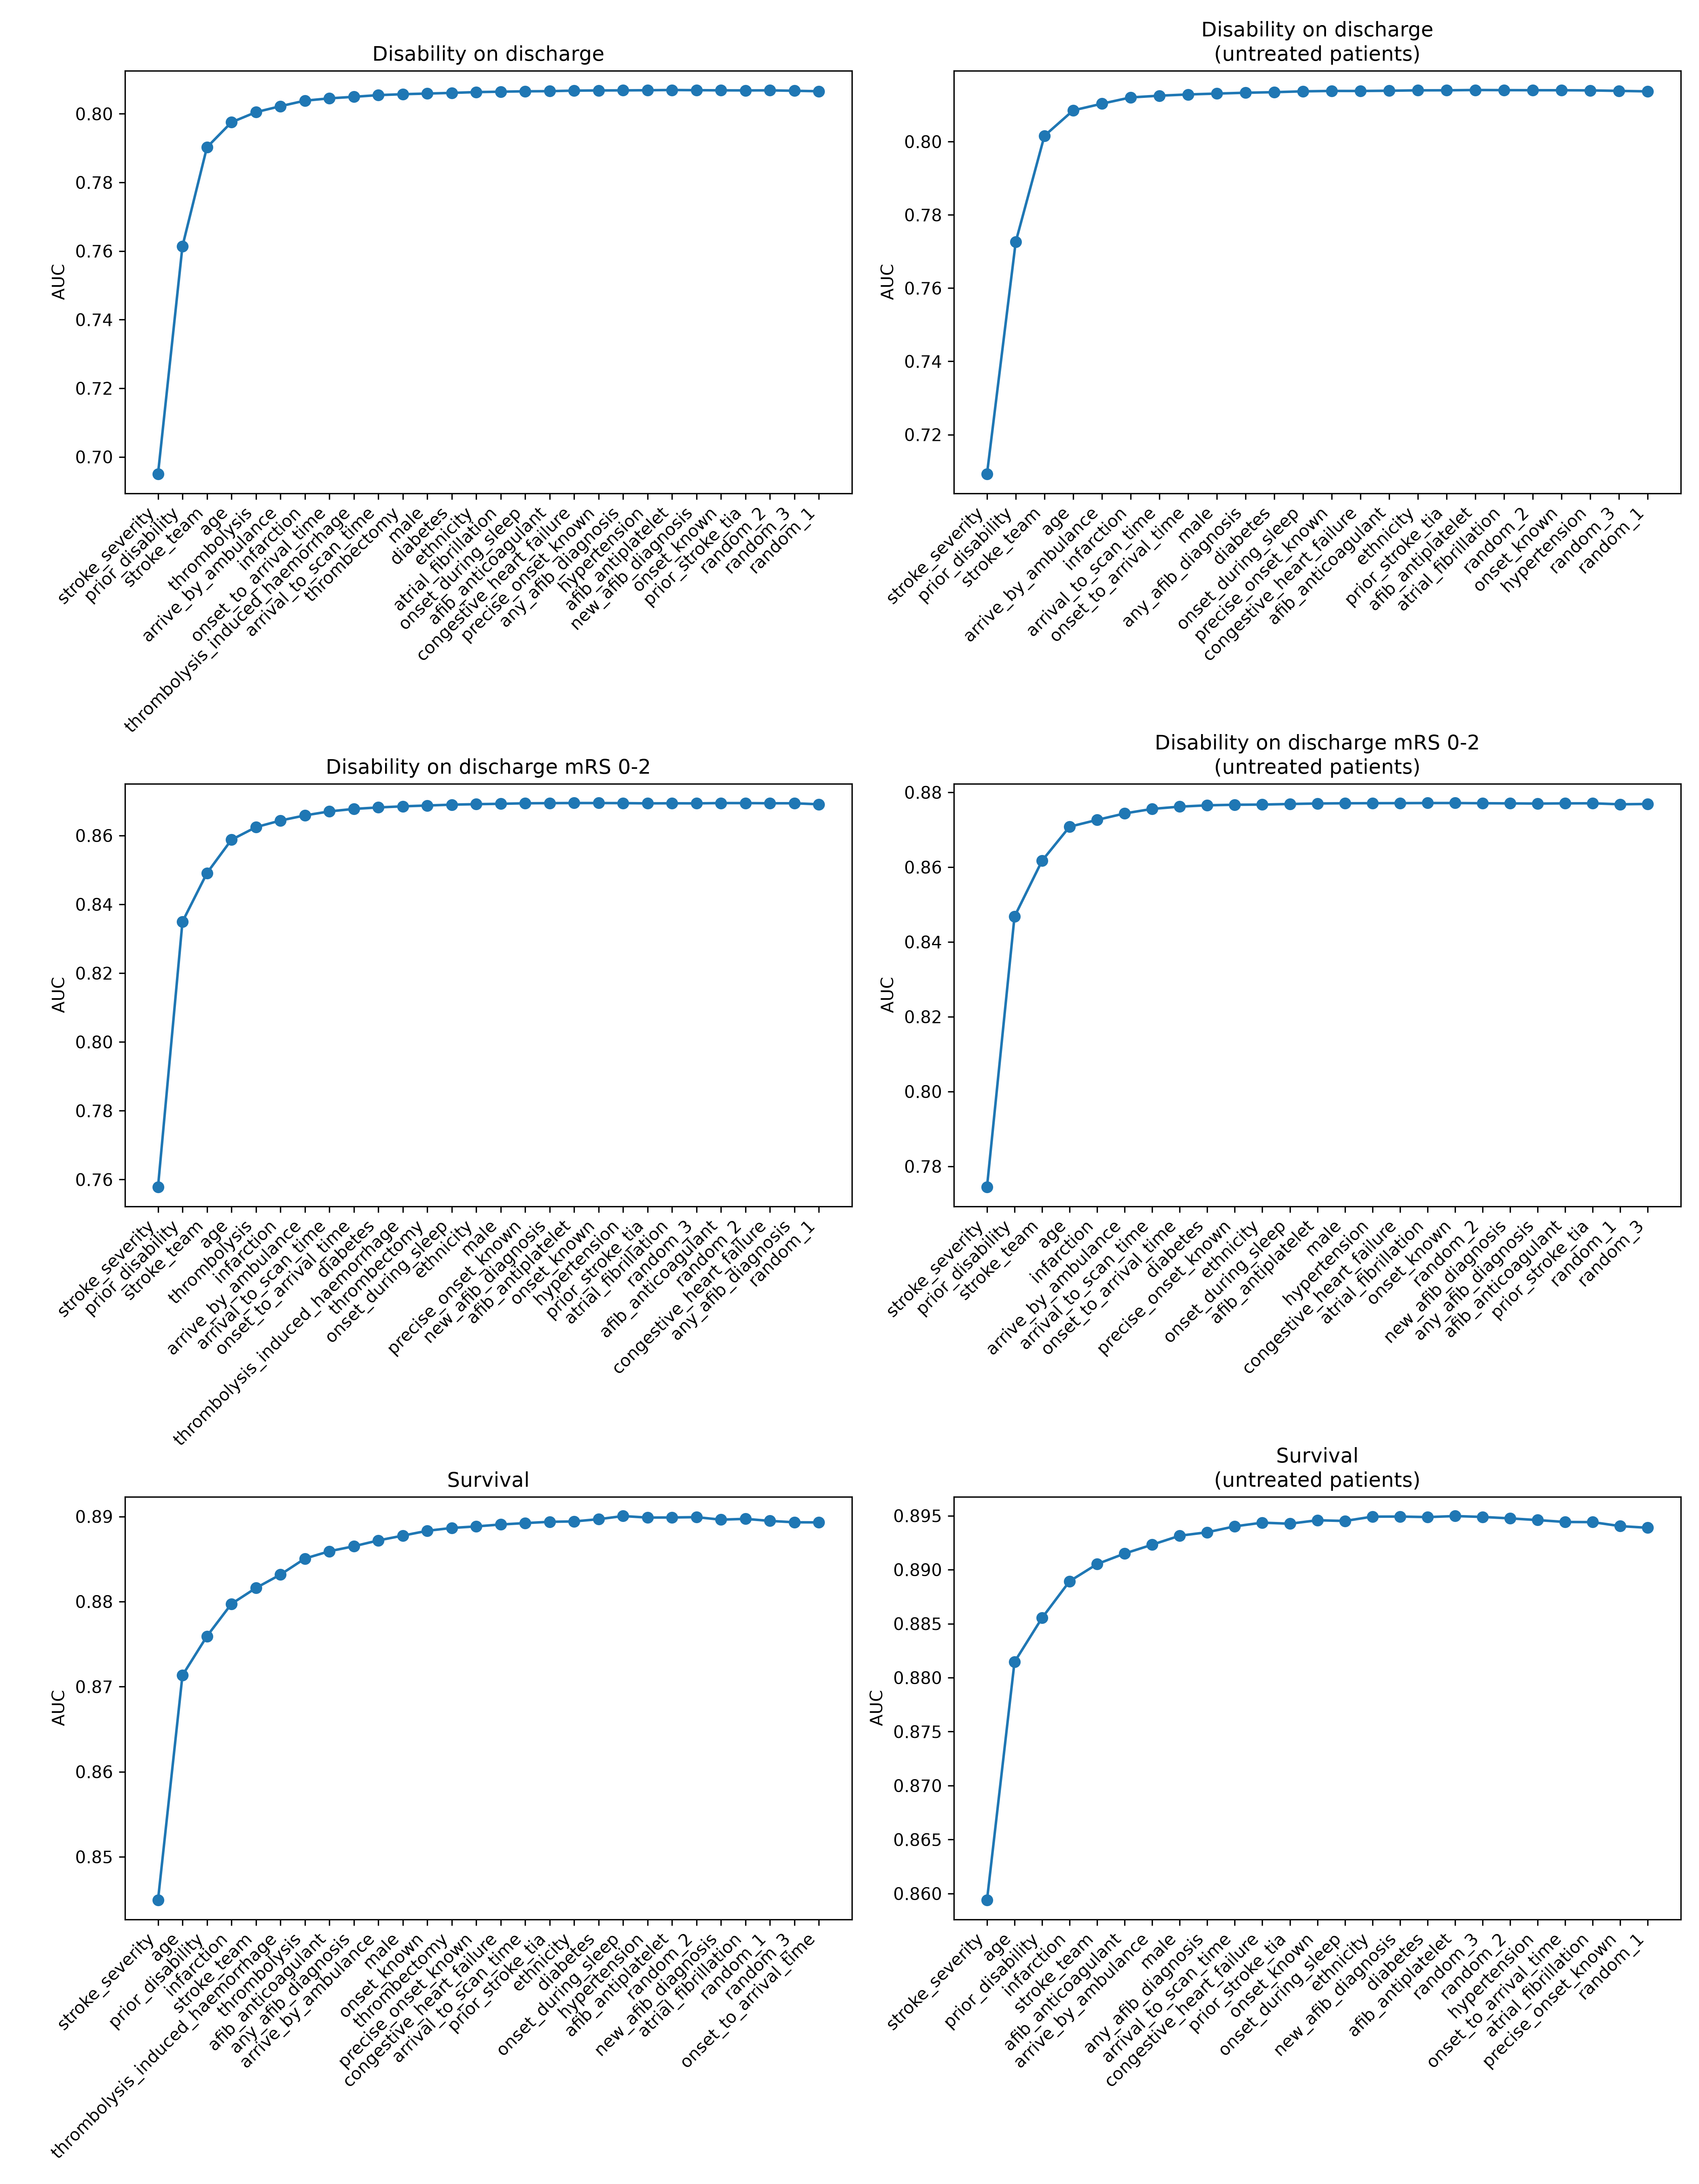
\includegraphics[width=0.98\linewidth]{images/feature_selection/feature_selection_1.png}
    \caption{Feature selection for XGBoost model. Features were selected based on Sequential Forward Selection (SFS) utilizing a greedy search algorithm. Results are shown for mRS disability at discharge for all patients, or those untreated with thrombolysis or thrombectomy (top row), disability at discharge being mRS 0-2 for all patients, or those untreated with thrombolysis or thrombectomy (middle row), and for survival until discharge (for all patients, or those untreated with thrombolysis or thrombectomy (bottom row).}
    \label{fig:feature_selection_1}
\end{figure}

\begin{figure}
    \centering
    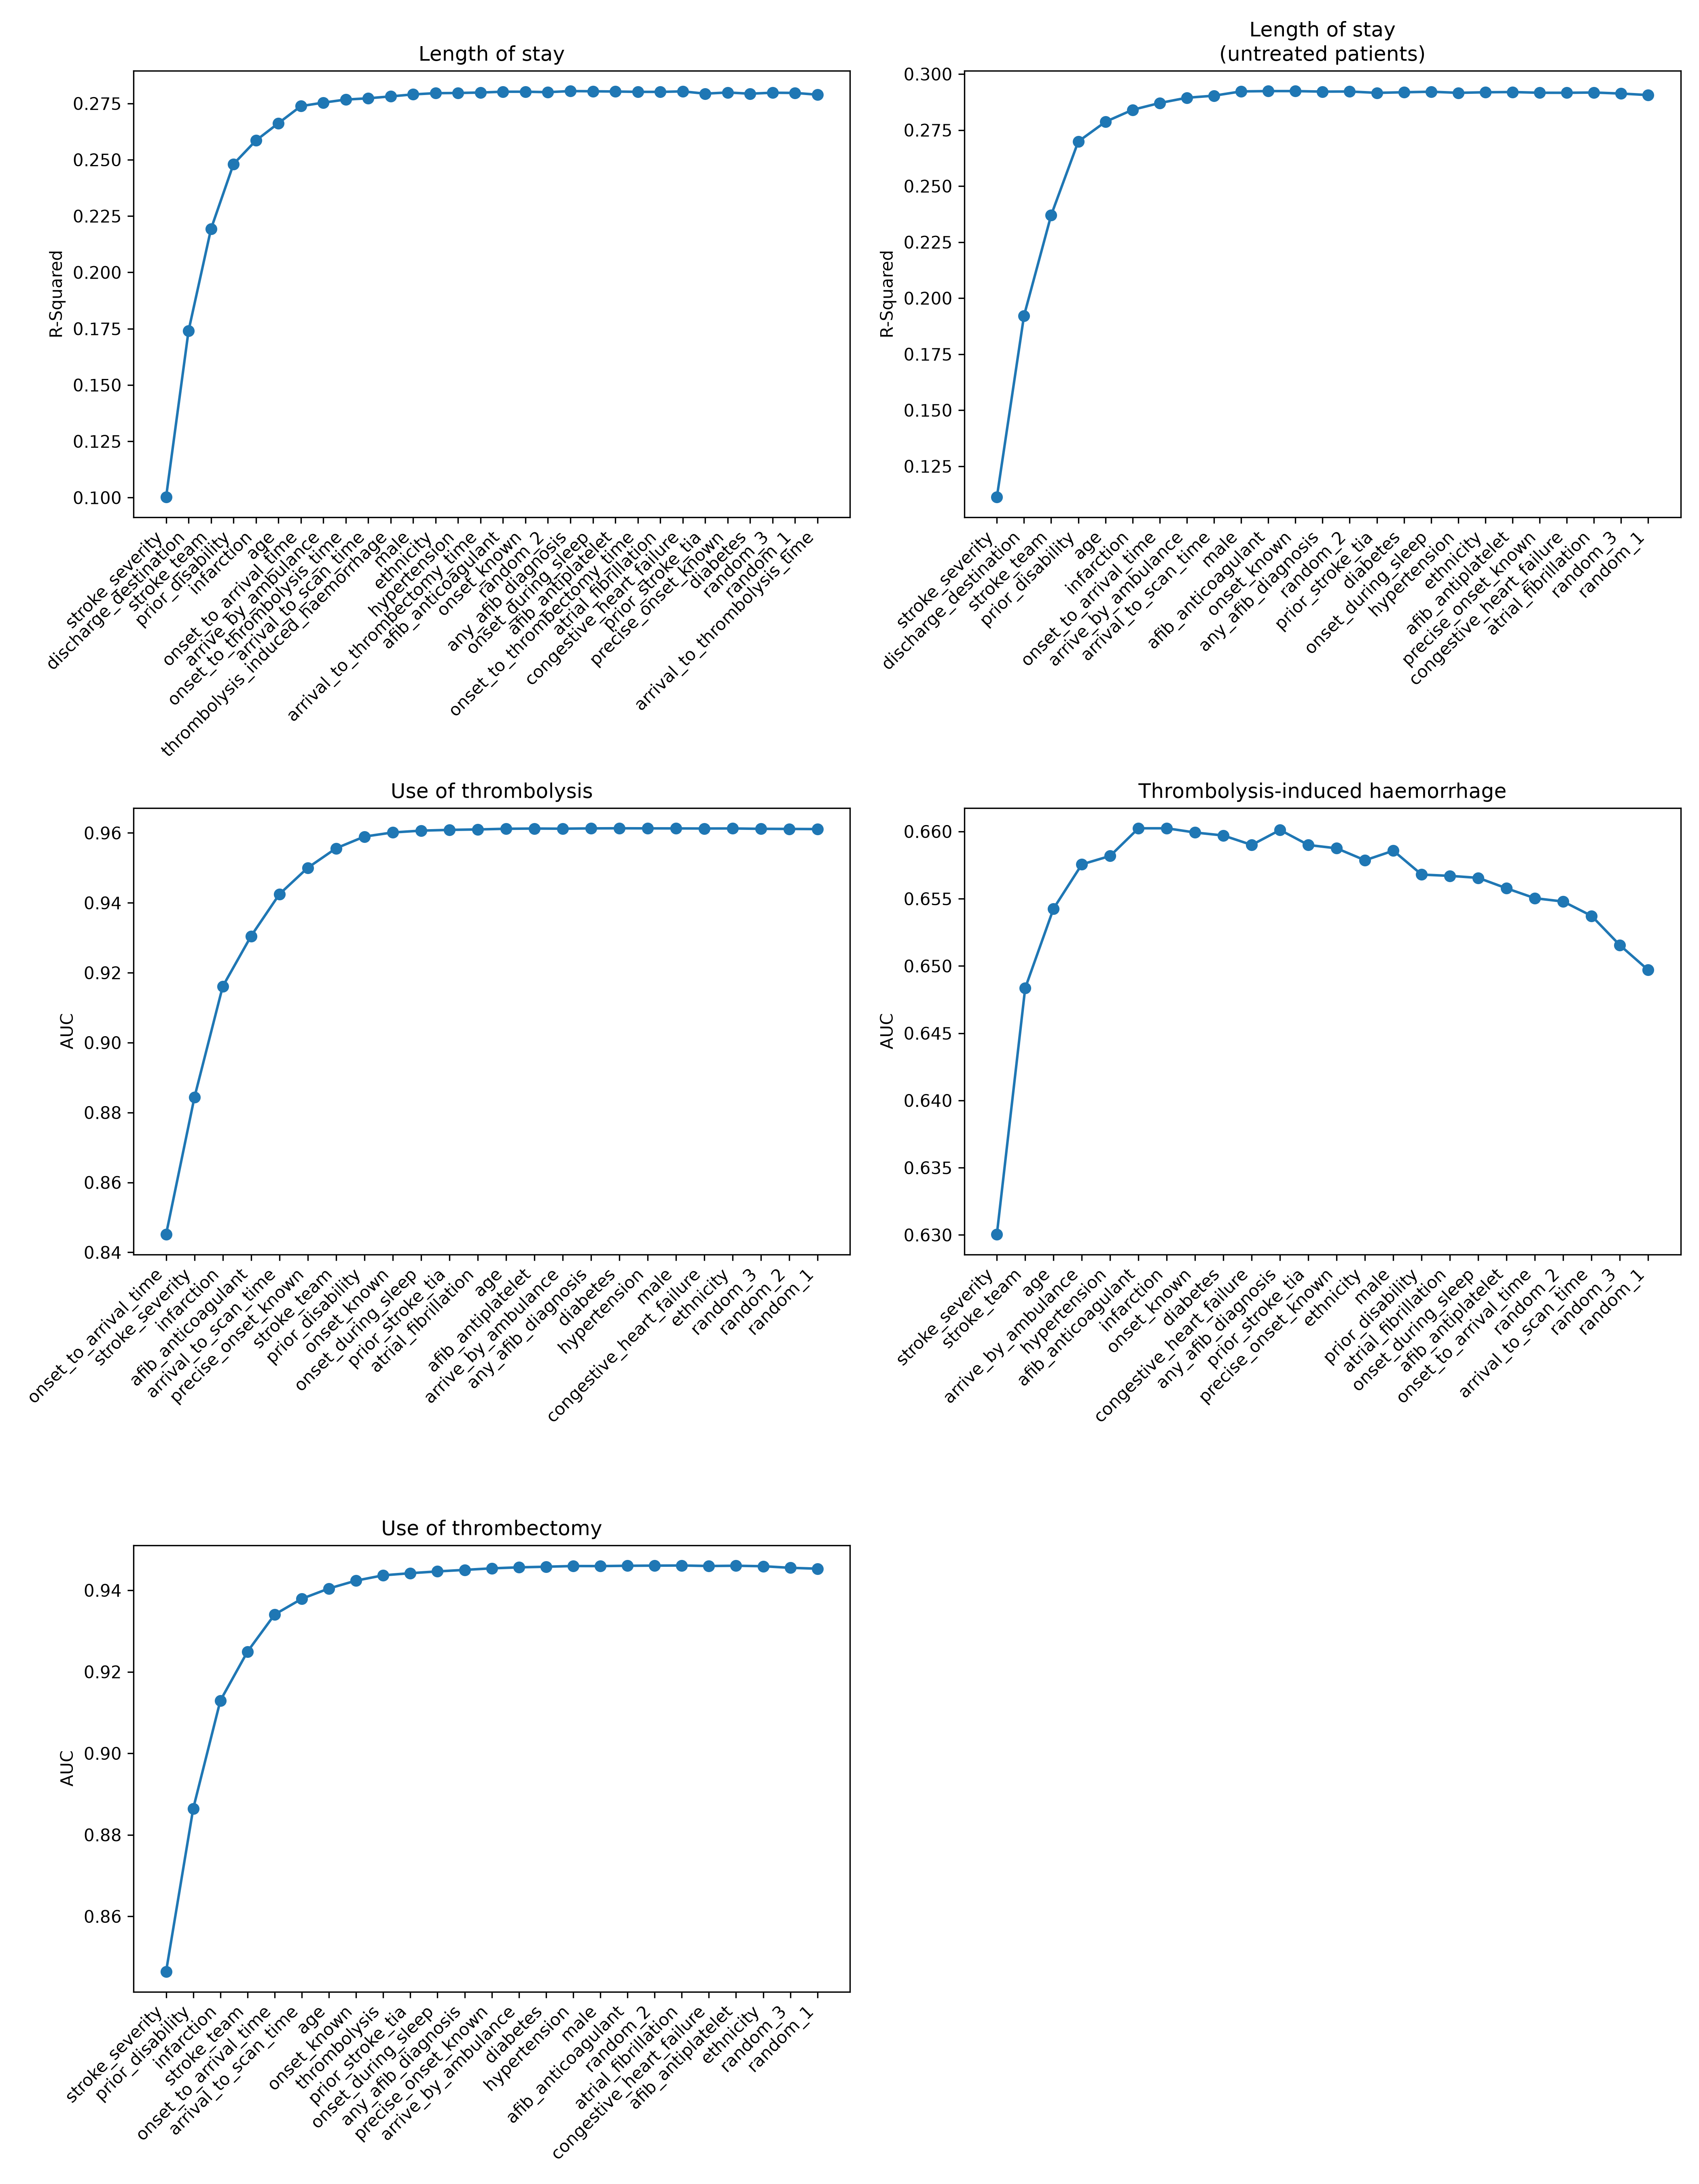
\includegraphics[width=0.98\linewidth]{images/feature_selection/feature_selection_2.png}
    \caption{Feature selection for XGBoost model. Features were selected based on Sequential Forward Selection (SFS) utilizing a greedy search algorithm. Results are shown for length of stay for all patients, or those untreated with thrombolysis or thrombectomy (top row), use of thrombolysis in all patients (middle row, left), thrombolysis-induced haemorrhage in patients receiving thrombolysis (middle row, right), and use of thrombectomy in all patients (bottom row).}
    \label{fig:feature_selection_2}
\end{figure}

% ====================================================================================

\newpage

\section{SHAP analysis}

Figures \ref{fig:shap_mrs0-2_all} to \ref{fig:shap_thrombectomy_all} show SHAP analysis for the different models. SHAP values quantify how each feature, given its specific value for an individual patient, contributed to that patient's model prediction. Each prediction is composed of two parts: a base value, common to all predictions from that model, and the sum of the SHAP values for every feature in that individual's case. Because the model allows for interactions between features, two patients with identical values for a given feature may still receive different SHAP values for that feature, depending on their other characteristics.

The units of the SHAP values depend on the type of model output. For binary outcomes (survival, discharge mRS 0-2, use of thrombolysis or thrombectomy, and thrombolysis-induced haemorrhage), SHAP values are expressed in log-odds; summing them with the base value yields the final log-odds prediction. For the continuous regression outcome (length of stay), SHAP values are expressed in the same units as the outcome itself (days).

In each figure, the top plot is a SHAP \textit{bee-swarm} plot. Feature values are colour-coded from blue (low) to red (high); for stroke severity, for example, blue points indicate low severity and red points indicate high severity. The position on the x-axis shows the SHAP value for each point, with points further to the left indicating that the feature is pushing the model's prediction lower (though this effect may be offset by other features, since SHAP values are additive). Points further to the right indicate the opposite: the feature is pushing the prediction higher. Features are ordered top-to-bottom by their overall importance - specifically, by the mean absolute SHAP value across all instances in the dataset, with the most influential feature at the top and the least influential at the bottom.

Below the top plot in each figure are two further plots showing the SHAP values for the two categorical features, ethnicity and stroke team. Because these features are categorical rather than continuous, they cannot be colour-coded by value in the same way as the bee-swarm plot above; instead, each category is shown separately. For each of the five ethnicity categories (Asian, Black, Mixed, Other/Not Known, White), the SHAP values for that feature—which will depend on interactions with other features—are shown as a violin plot combined with a box plot. The violin plot shows the full distribution and density of SHAP values within each category, while the overlaid box plot summarises this distribution using the median, interquartile range, and outliers, allowing comparison of both central tendency and spread across ethnicity or stroke team categories.SHAP values for stroke teams are shown as a bar chart, with one bar per stroke team representing that team's average SHAP value across all its patients. Bars are ordered from highest to lowest SHAP value, so that teams associated with the largest positive contribution to the model's prediction appear at one end, and those with the largest negative contribution appear at the other.

Though SHAP adds explainability to the model, care should be taken remembering that SHAP values show the influence of a feature value to the final prediction, but that this relationship is not necessarily causal (just as nicotine-stained fingernails may indicate high risk of lung cancer, but the stained nails do not cause the lung cancer). These models and plots are exploratory work, investigating which features may need to be included in later causal models.

Some observations may be made:

\textbf{Prediction of favourable outcome (mRS 0-2) at discharge} (figure \ref{fig:shap_mrs0-2_no_all}): Lower disability outcomes were especially associated with lower stroke severity, lower prior disability, and lower age. Ischaemic stroke patients had a lower chance of favourable outcomes, compared to haemorrhagic stroke (if all other feature values were similar). The stroke team attended also significantly affected the odds of being discharged mRS 0-2. Black and Asian patients had somewhat lower odds of being discharged mRS 0-2. Lower time to thrombolysis or thrombectomy improved the odds of being discharged mRS 0-2, but longer times to treatment worsened those odds compared to untreated patients. Figure \ref{fig:shap_mrs0-2_no_treatment} repeated the modelling, but for patients not treated with thrombolysis or thrombectomy, confirming that stroke severity, age, prior disability, stroke team and stroke type were the most important features affecting odds of being discharged mRS 0-2, independent of treatment.

\textbf{Prediction of survival until discharge} (figure \ref{fig:shap_survival_all}): Survival was especially associated with lower stroke severity, lower age, and lower prior disability. The stroke team attended also significantly affected the odds of survival. Ischaemic stroke patients had a lower chance of survival, compared to haemorrhagic stroke (if all other feature values were similar). Black, Asian, and Mixed ethnicity patients had \textit{higher} odds of survival compared to white patients (but, as we previously said, with lower odds of being discharged disability-free). Figure \ref{fig:shap_survival_no_treatment} repeated the modelling, but for patients not treated with thrombolysis or thrombectomy, confirming that stroke severity, age, prior disability, stroke team and stroke type were the most important features affecting odds of being discharged mRS 0-2, independent of treatment.

\textbf{Prediction of length of stay} (figure \ref{fig:shap_los_all}): Higher stroke severity was associated with longer lengths of stay, though dying in hospital was associated with shorter lengths of stay, as was being discharged to a community or early-supported discharge team. Stoke team had a significant effect on prediction of length of stay. Shorter onset-to-arrival times were associated with lower lengths of stay.

\textbf{Use of thrombolysis} (figure \ref{fig:shap_thrombolysis_all}): Key features associated with higher odds of use of thrombolysis were: shorter onset-to-arrival and arrival-to-scan times, infarction stroke, higher stroke severity, no use of atrial fibrillation anticoagulation, and lower prior disability. Odds of receiving thrombolysis were slightly lower in Black and Mixed ethnicity groups. Stroke team attended had a significant association with odds of receiving thrombolysis.

\textbf{Use of thrombectomy} (figure \ref{fig:shap_thrombectomy_all}): Key features associated with higher odds of use of thrombolysis were: higher stroke severity, infraction stroke, shorter onset-to-arrival and arrival-to-scan times, lower prior disability, and lower age. Odds of receiving thrombectomy were  lower in Black, Asian and and Mixed ethnicity groups. Stroke team attended had a significant association with odds of receiving thrombectomy.

\textbf{Thrombolysis-induced haemorrhage, in patients receiving thrombolysis} (figure \ref{fig:shap_thrombolysis_haemorrhage}): Though this model had lower predictive scores, SHAP is included here for completeness. Odds of thrombolysis causing haemorrhage were higher with shorter onset-to-arrival times, higher stroke severity, lower arrival-to-scan times, and lower pre-stroke disability. Stroke team attended had a significant association with odds of thrombolysis-induced haemorrhage.

%%%%%%%%%%% Discharge disability 0-2 %%%%%%%%%%%%%%%

%% All patients

\begin{figure}[htbp]
    \centering
    
    % Top image (Full width)
    \begin{subfigure}{0.50\textwidth}
        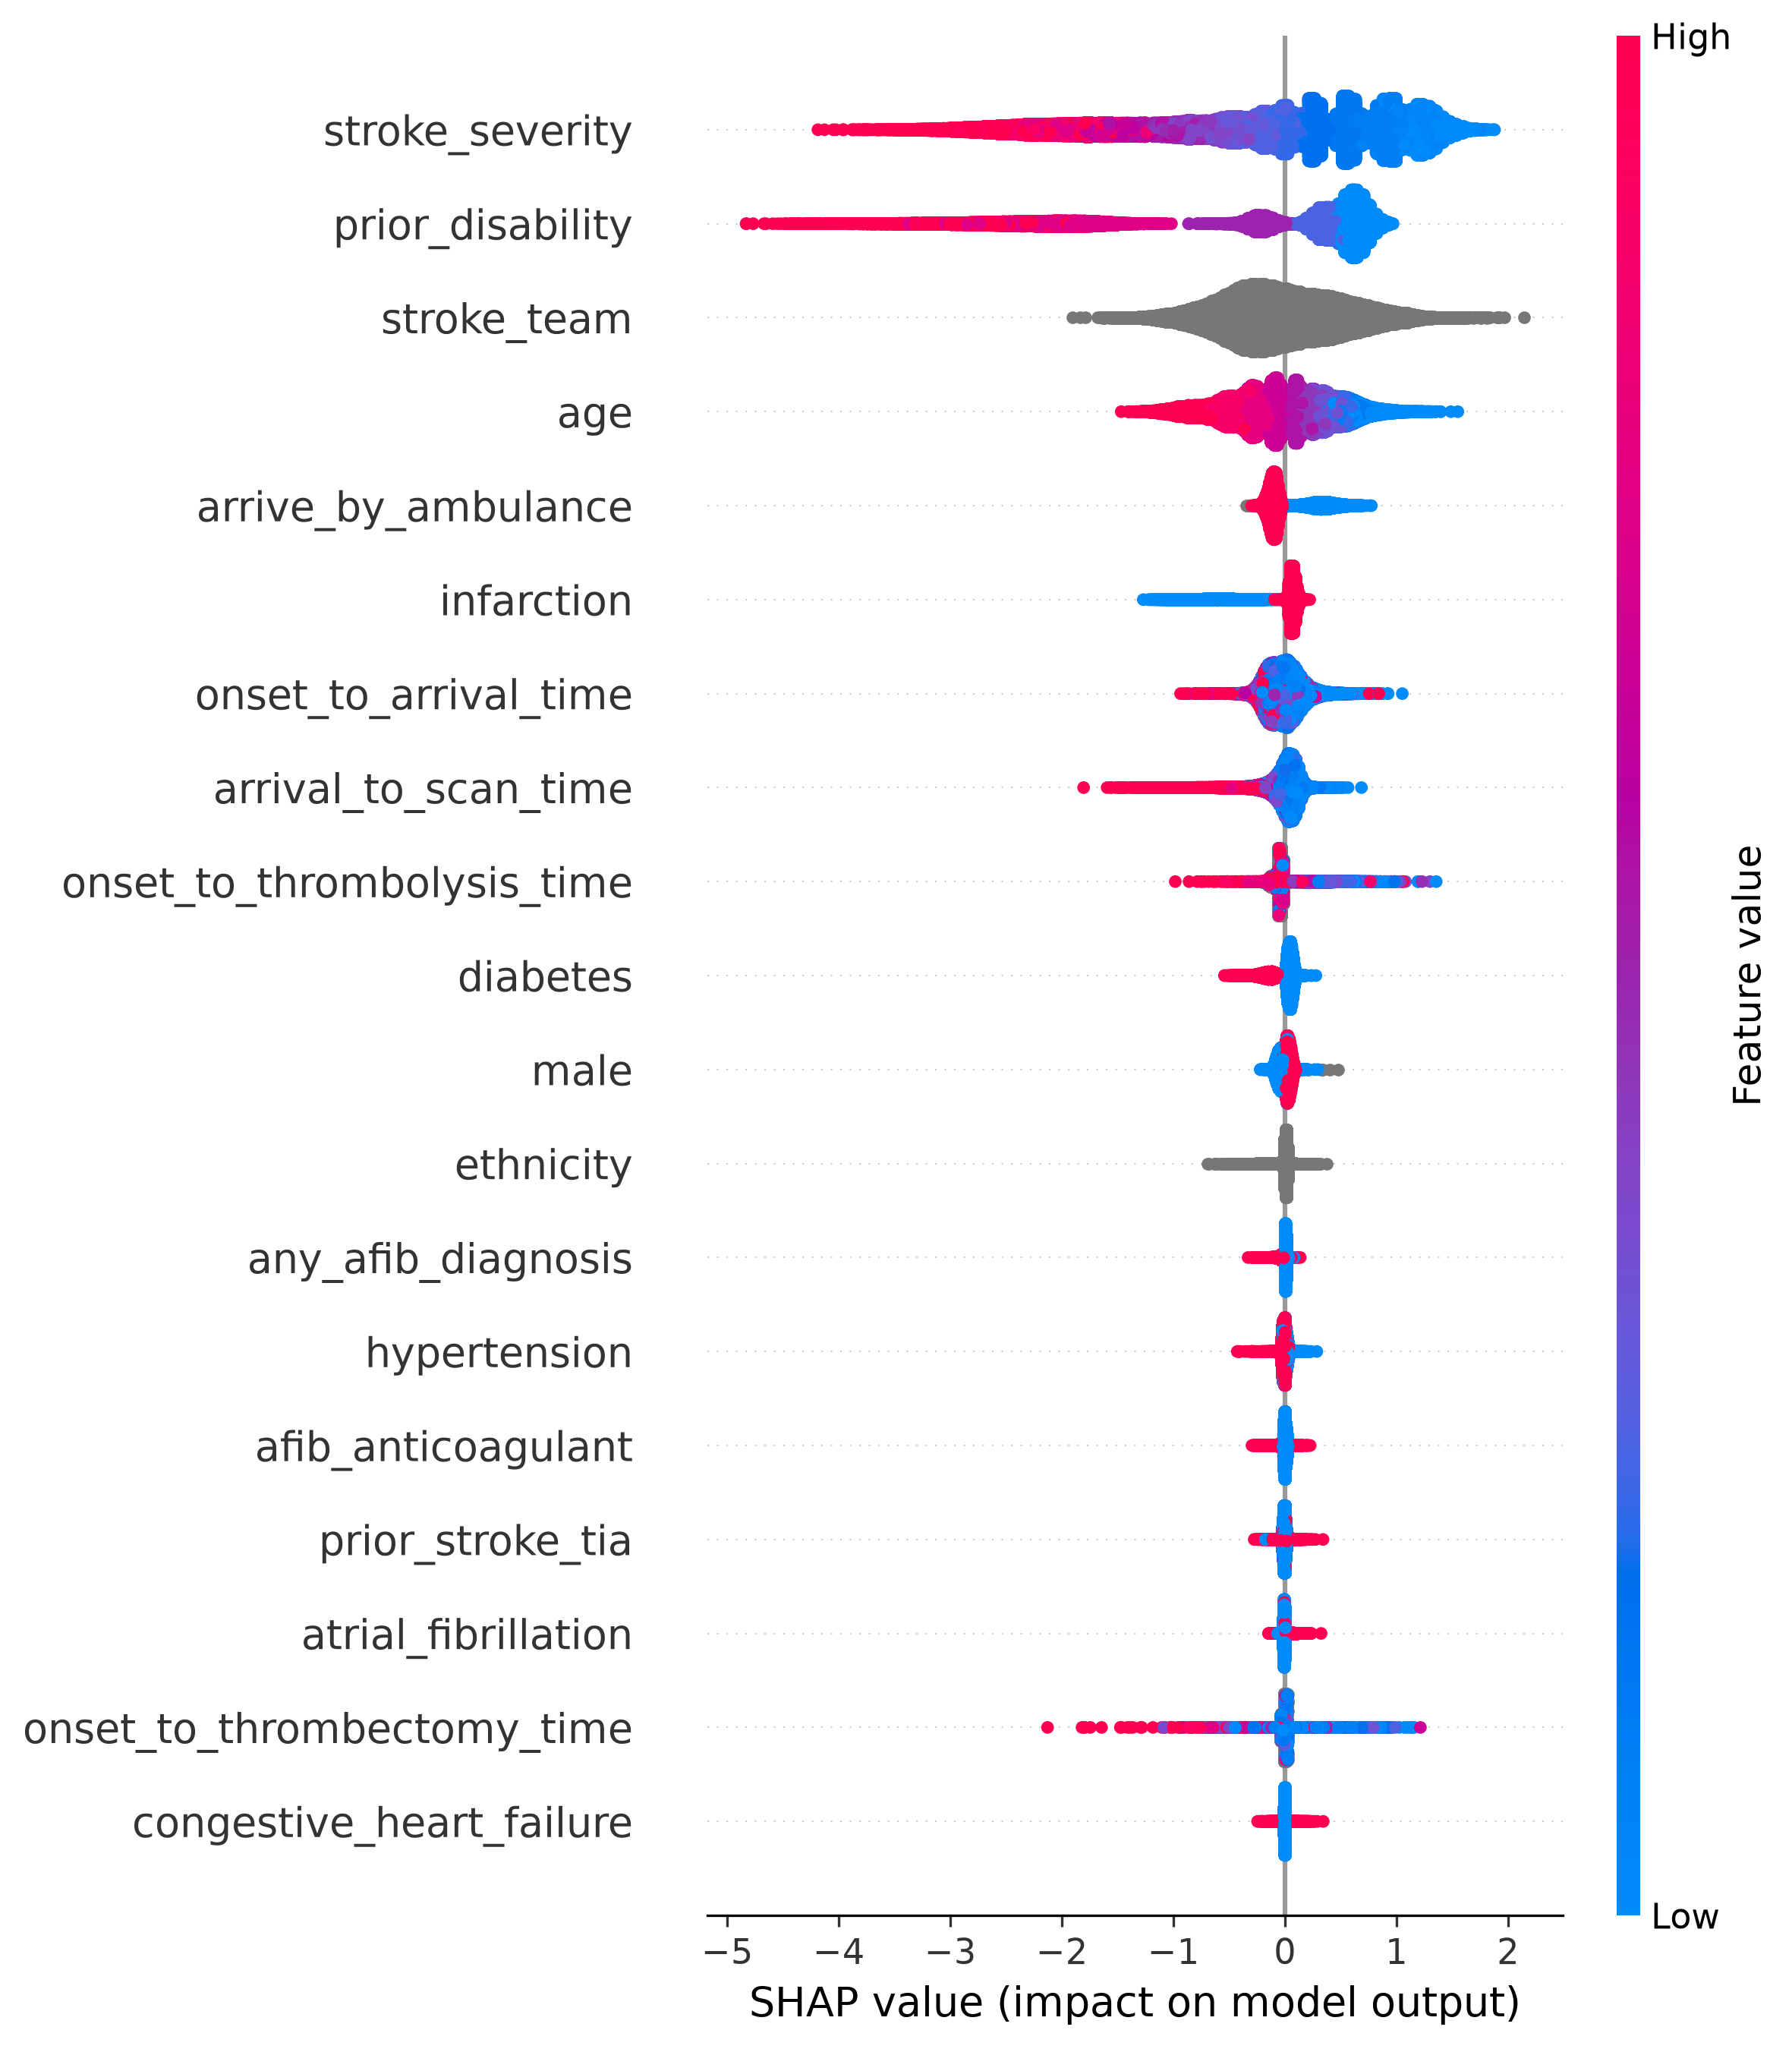
\includegraphics[width=\linewidth]{images/shap/shap_all_patients_mrs_less_than_3.png}
        %\caption{}
        \label{fig:top}
    \end{subfigure}

    \vspace{0.5cm} % Optional vertical space between rows

    % Bottom left image (~45% width)
    \begin{subfigure}{0.407\textwidth}
        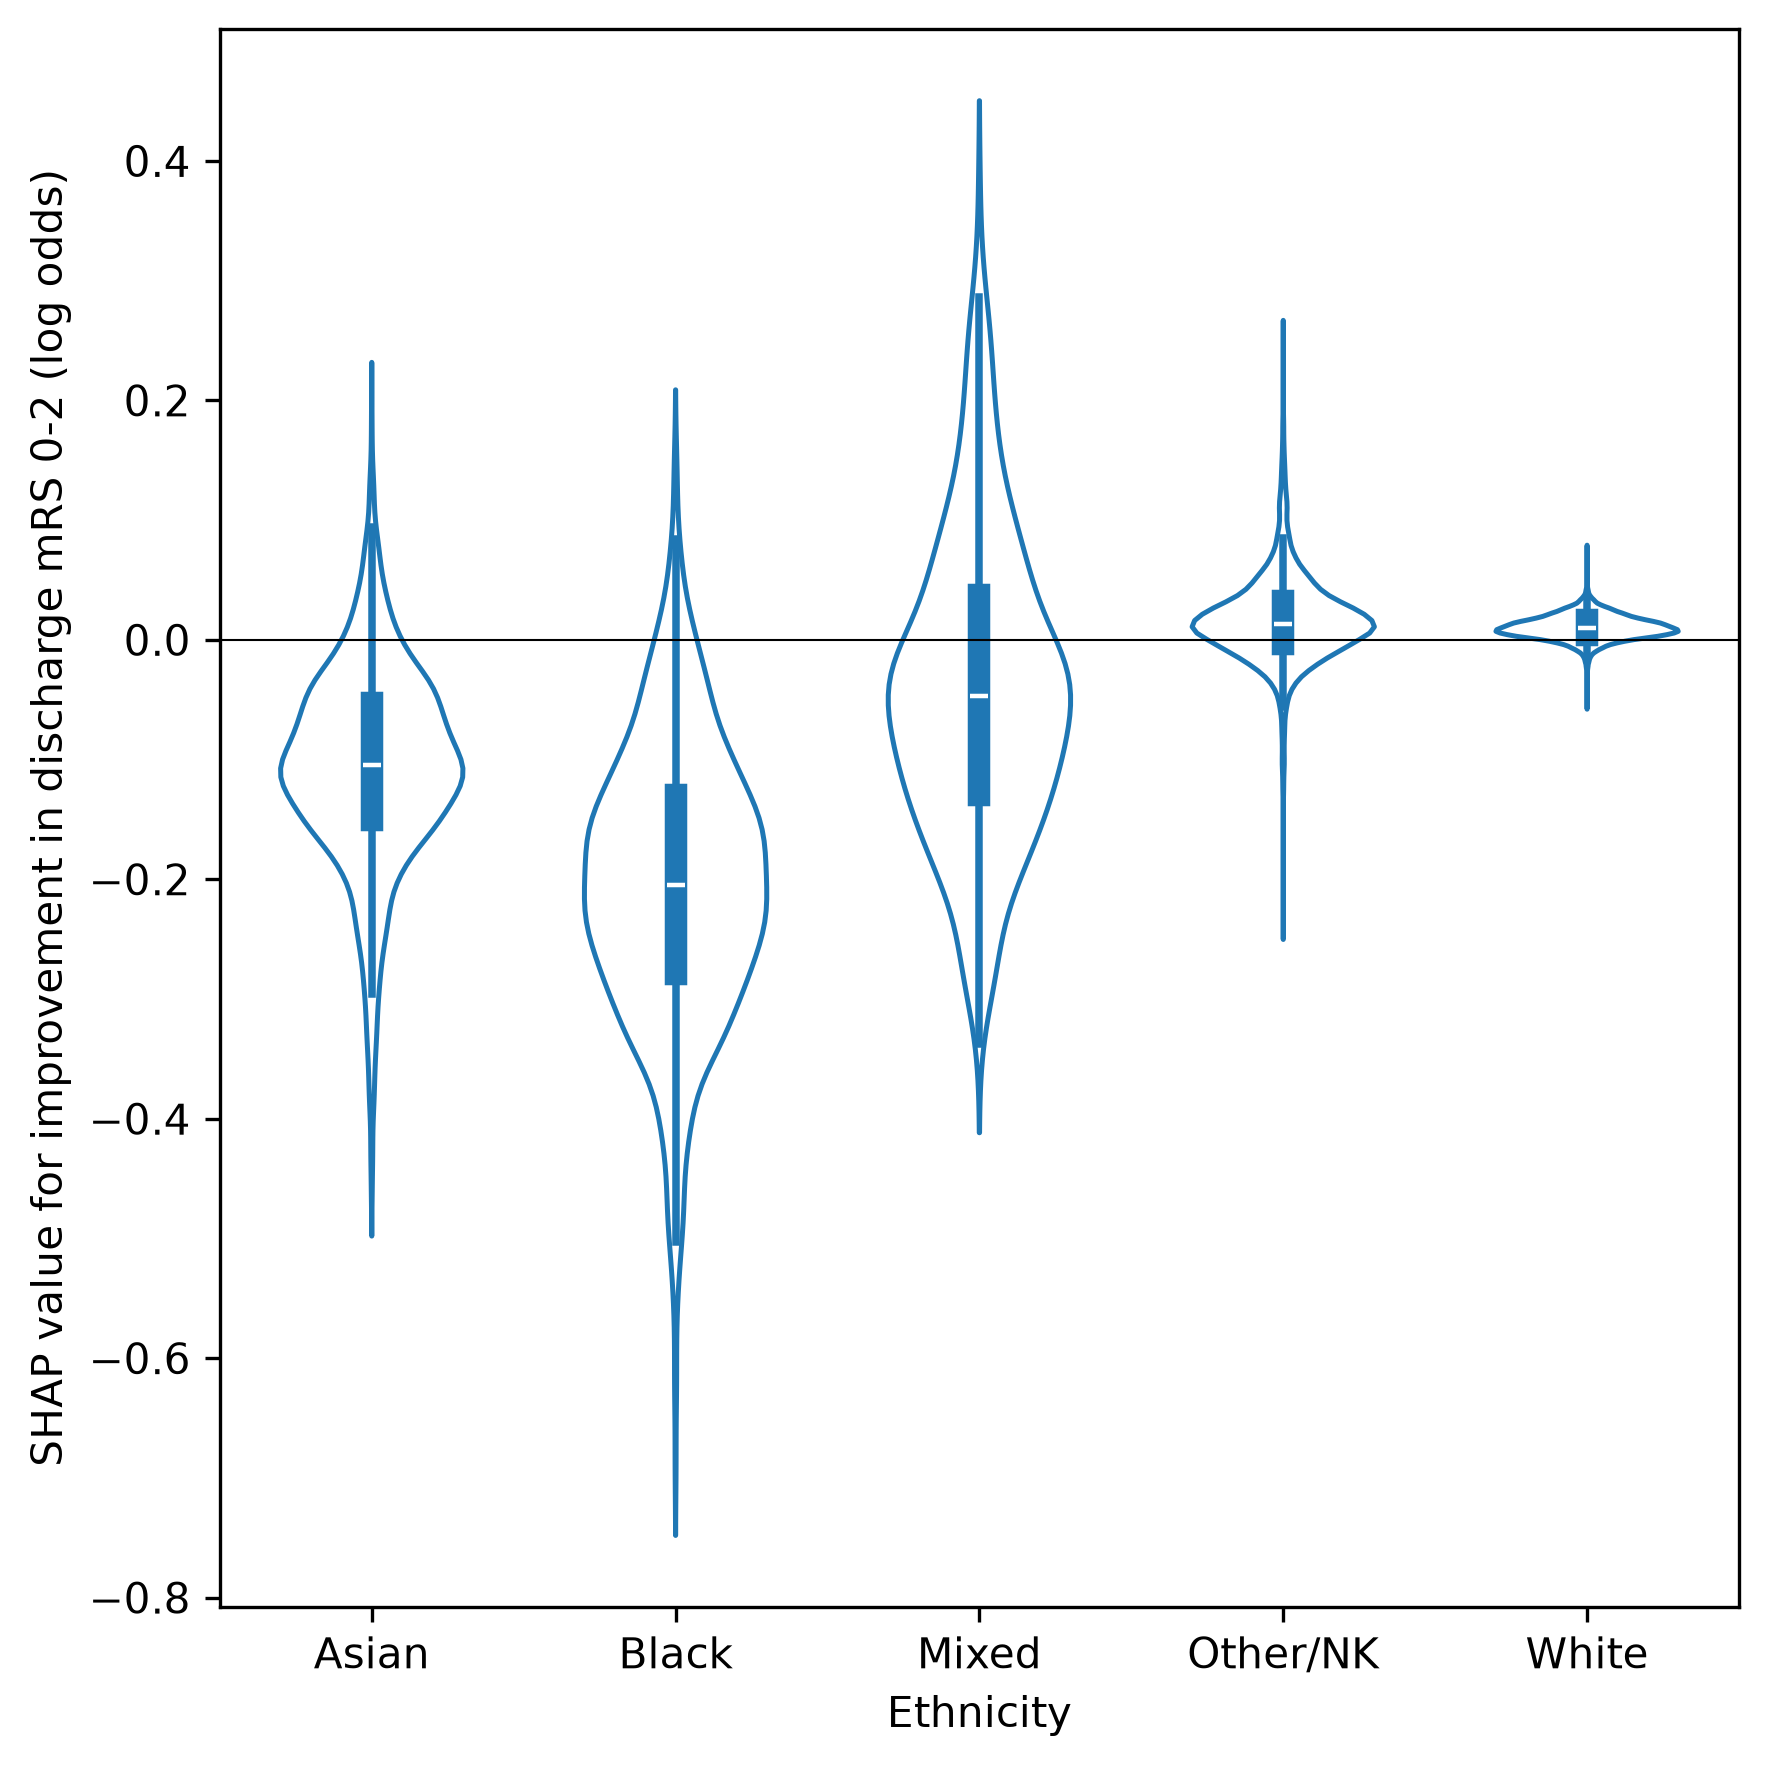
\includegraphics[width=\linewidth]{images/shap/shap_all_patients_mrs_less_than_3_ethnicity.png}
        %\caption{}
        \label{fig:bottom-left}
    \end{subfigure}
    \hfill % Adds flexible horizontal spacing
    % Bottom right image (~55% width)
    \begin{subfigure}{0.543\textwidth}
        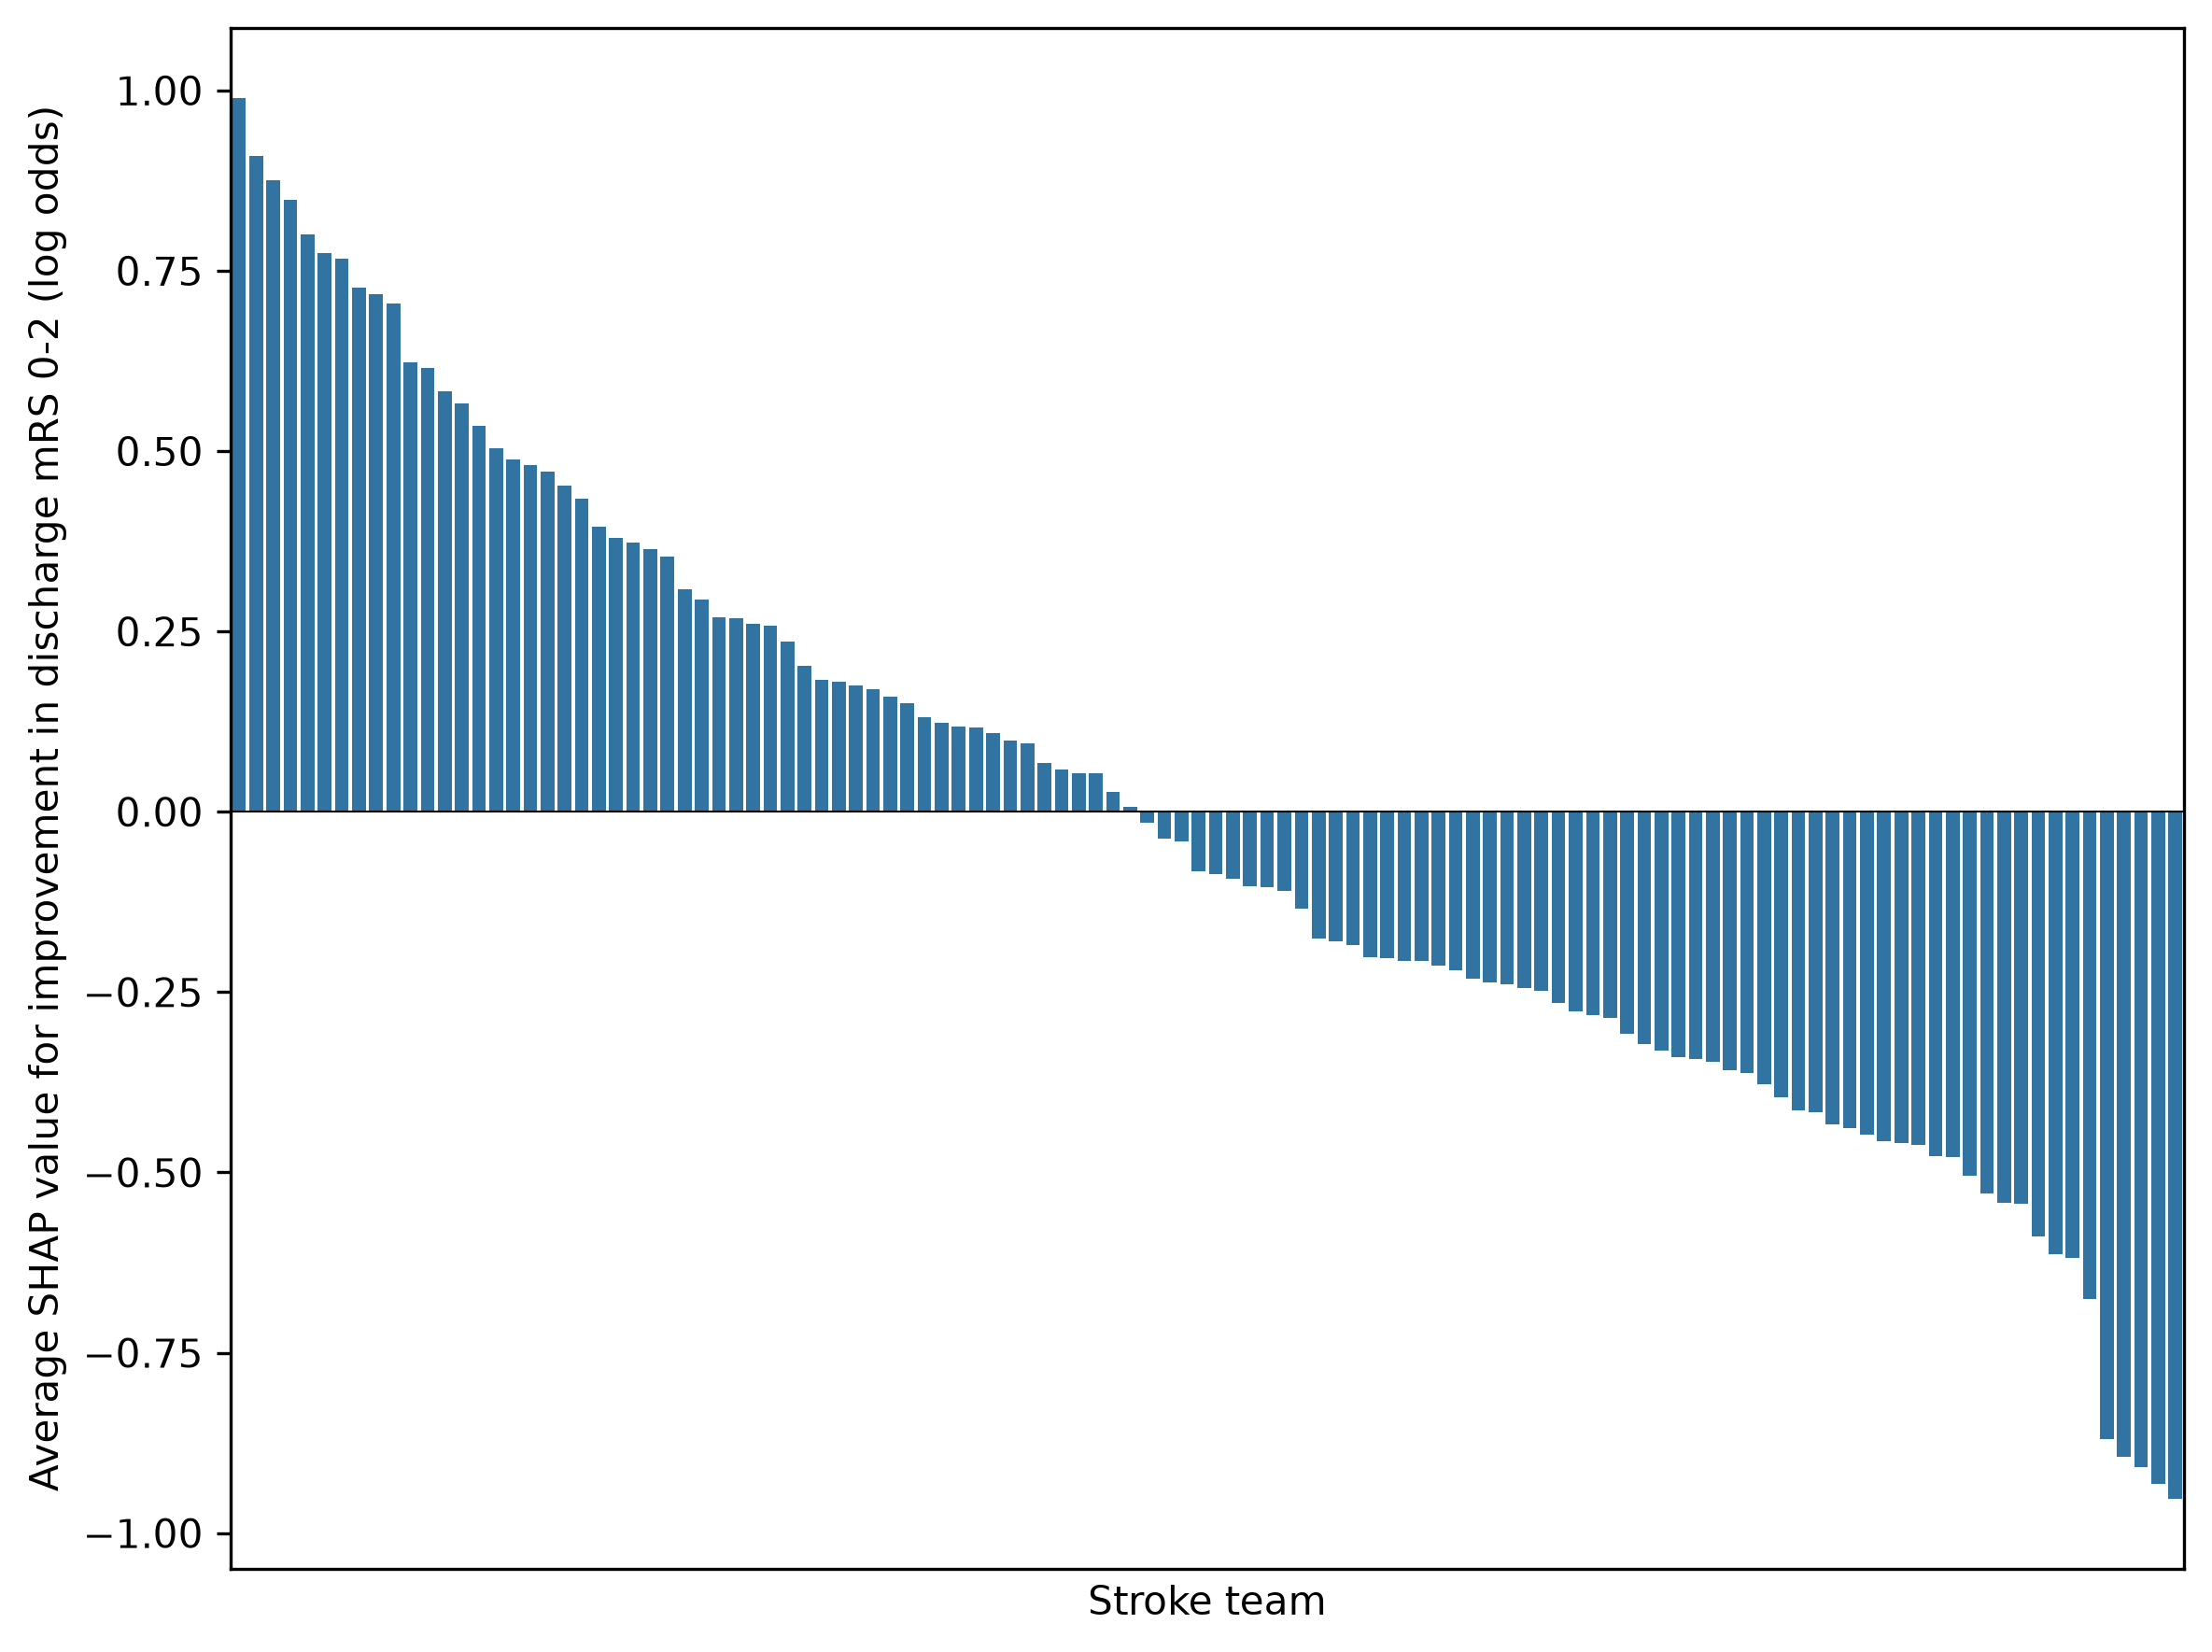
\includegraphics[width=\linewidth]{images/shap/shap_all_patients_mrs_less_than_3_stroke_team.png}
        %\caption{}
        \label{fig:bottom-right}
    \end{subfigure}

    \caption{SHAP analysis of feature contributions to predicting favourable discharge outcomes (mRS 0-2) in stroke patients. \textit{Top}: A SHAP summary plot detailing the impact of features on the model's log-odds predictions. Each point represents an individual patient instance. The position on the x-axis indicates the SHAP value, where positive values increase the predicted odds of a favourable outcome, and negative values decrease it. For continuous and binary variables, colour represents the original feature value (red indicating high values; blue indicating low values). Categorical variables (\textit{stroke team} and \textit{ethnicity}) are plotted in grey. \textit{Bottom left}: Violin plots illustrating the distribution of SHAP values across distinct ethnic groups. This panel highlights the marginal impact and variance of ethnicity on the model’s prediction for disability outcome. \textit{Bottom Right}: A ranked bar chart displaying the average SHAP value associated with each individual stroke team. This panel visualizes institutional variation, reflecting the contribution of the treating stroke team to the predicted patient outcome after accounting for patient-level clinical characteristics.}
    \label{fig:shap_mrs0-2_all}
\end{figure}

%% Untreated patients

\begin{figure}[htbp]
    \centering
    
    % Top image (Full width)
    \begin{subfigure}{0.50\textwidth}
        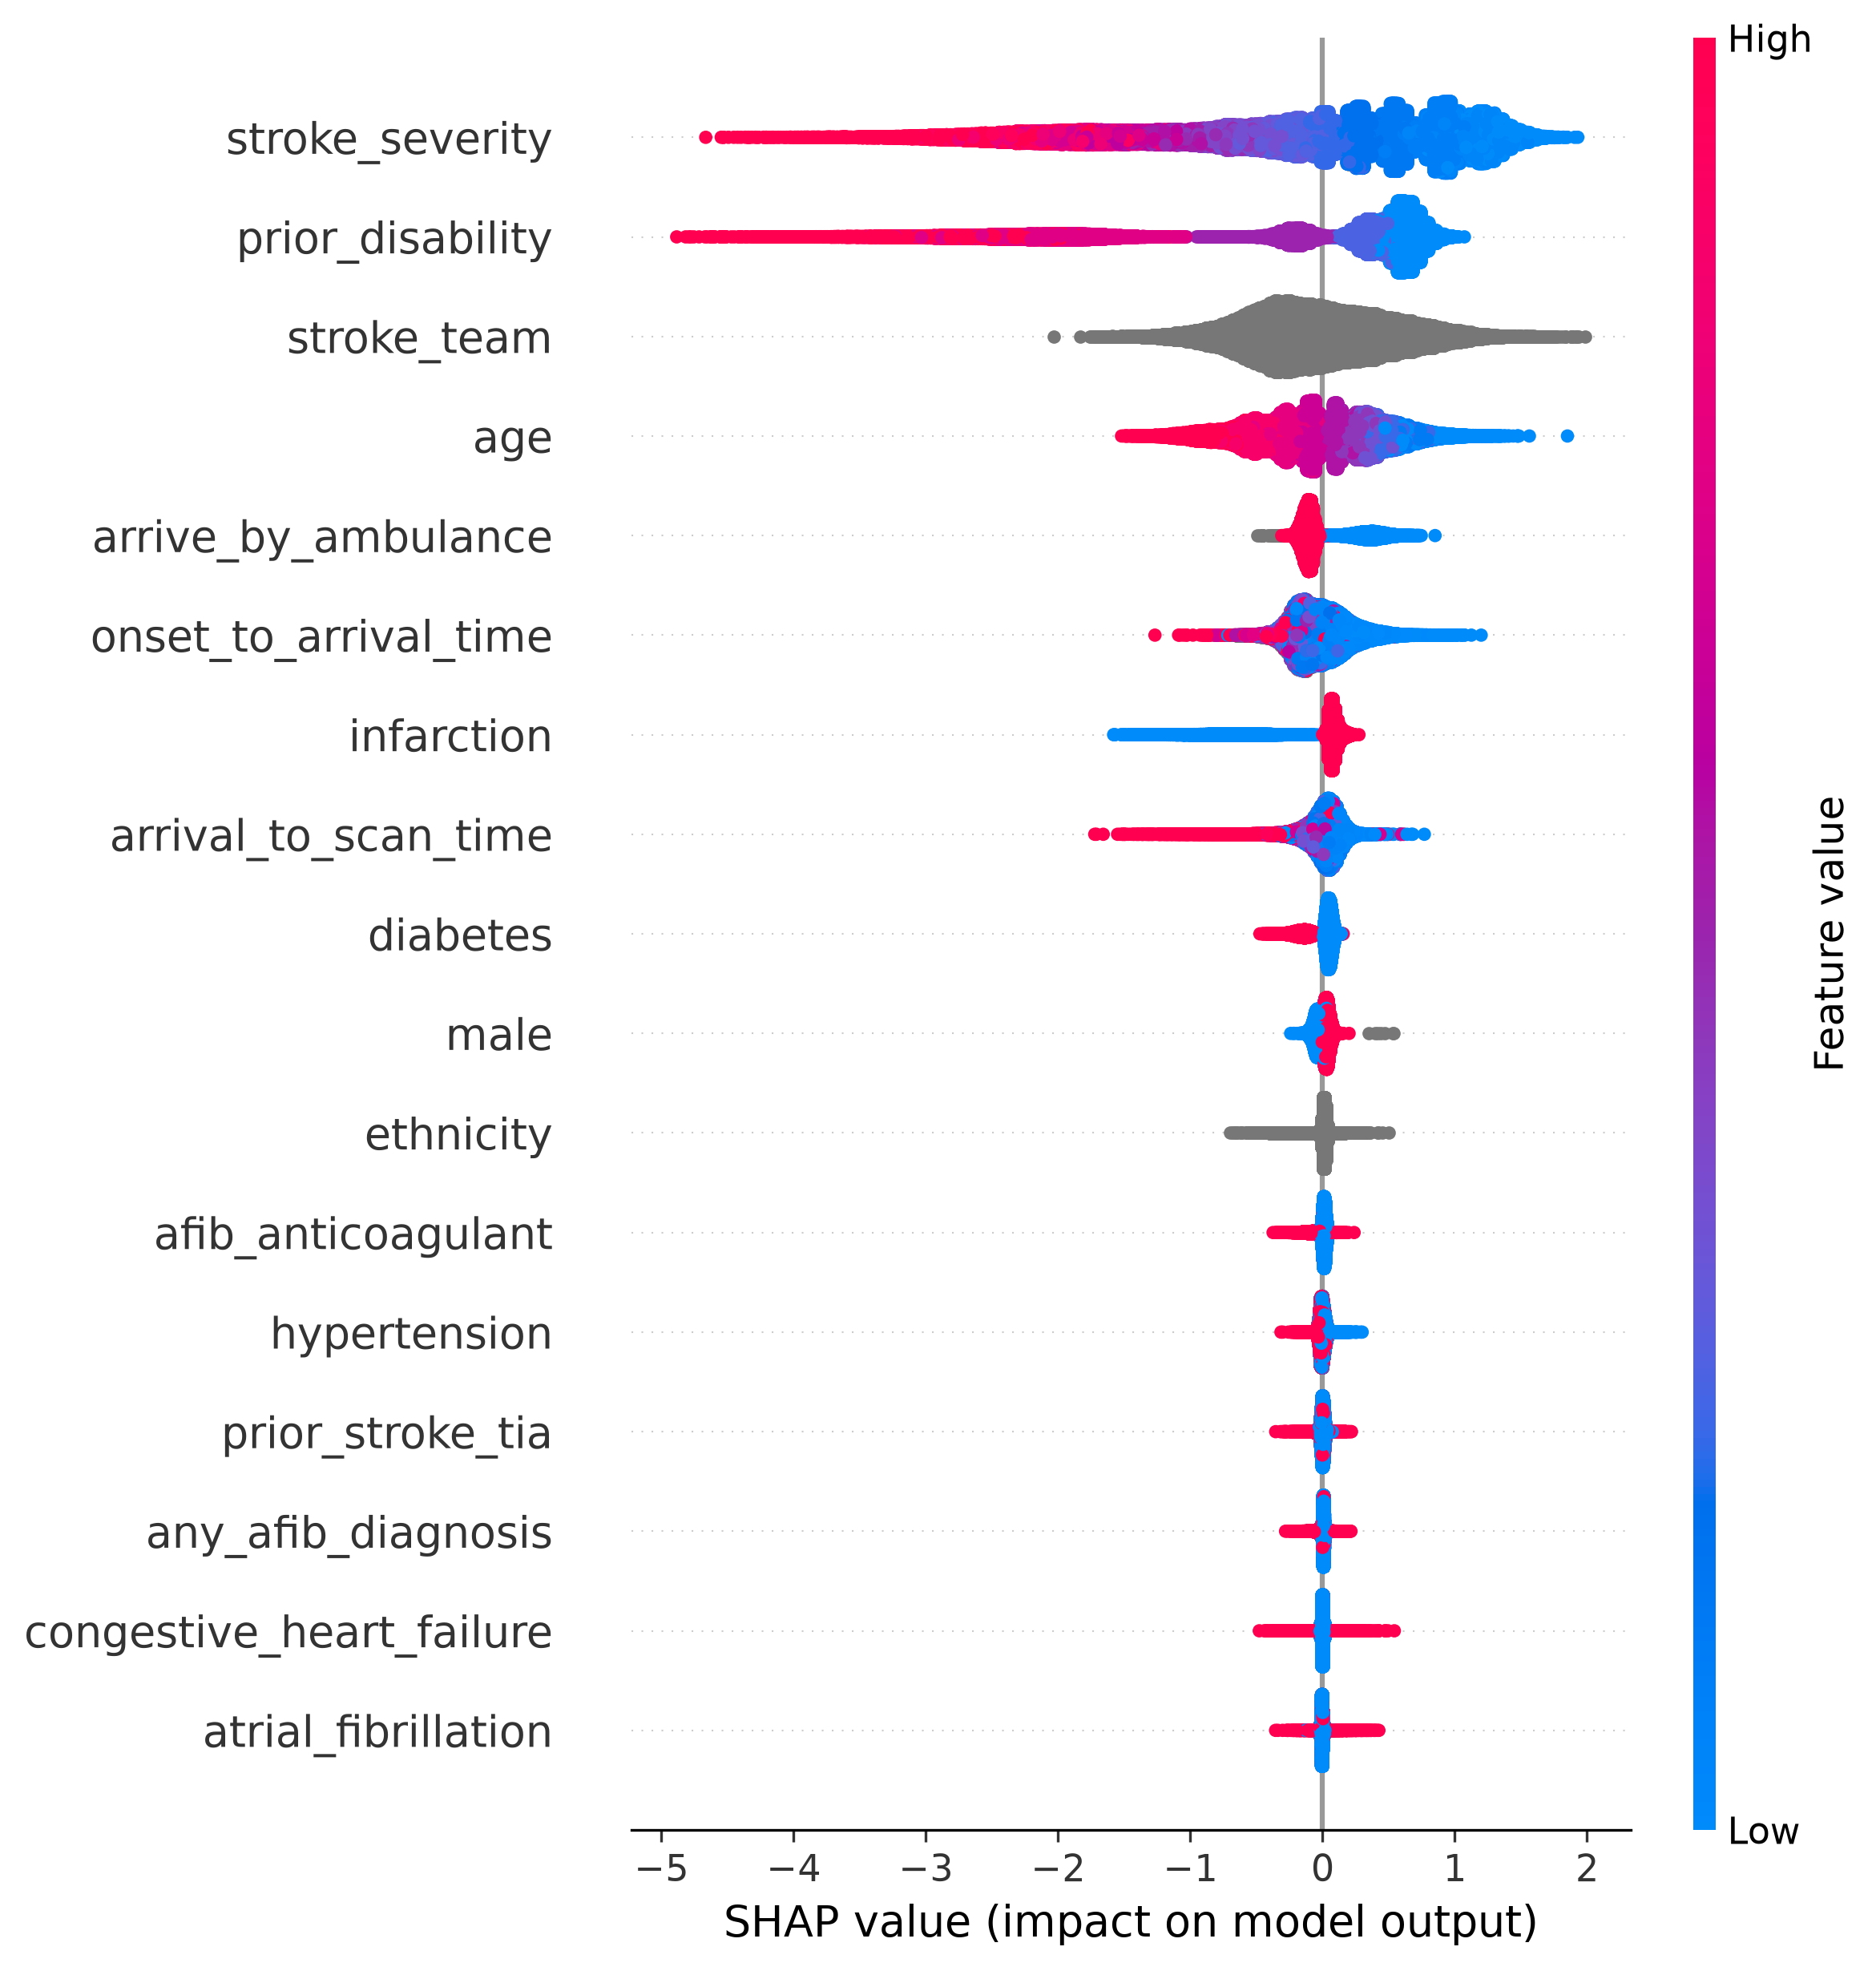
\includegraphics[width=\linewidth]{images/shap/shap_untreated_patients_mrs_less_than_3.png}
        %\caption{}
        \label{fig:top}
    \end{subfigure}

    \vspace{0.5cm} % Optional vertical space between rows

    % Bottom left image (~45% width)
    \begin{subfigure}{0.407\textwidth}
        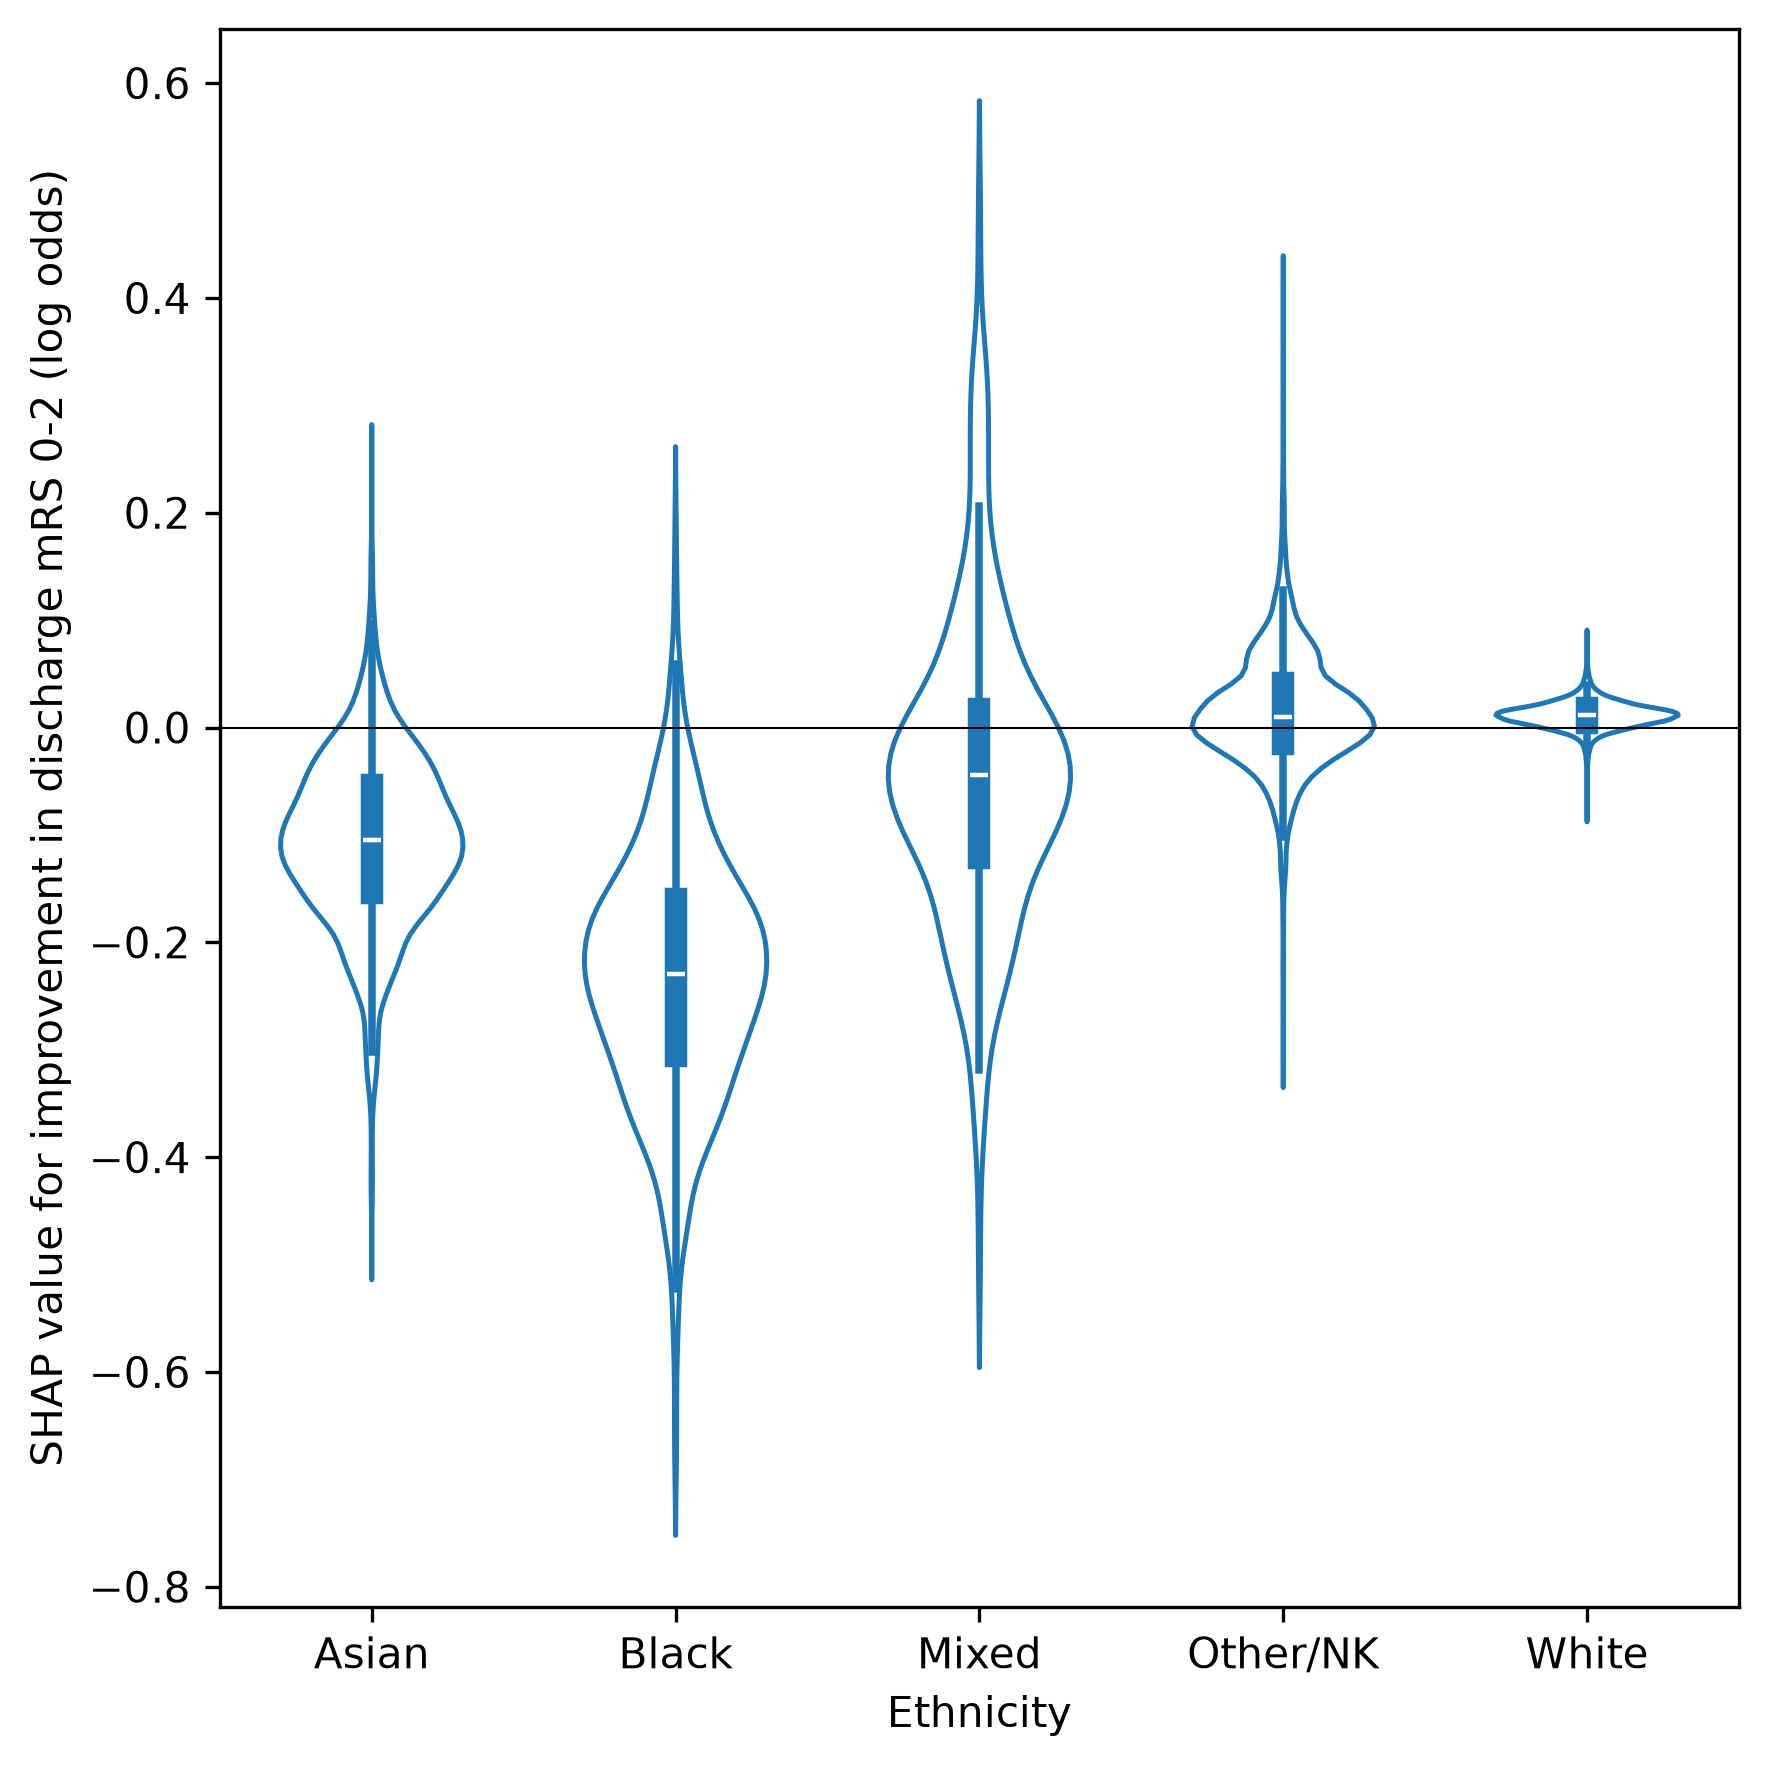
\includegraphics[width=\linewidth]{images/shap/shap_untreated_patients_mrs_less_than_3_ethnicity.png}
        %\caption{}
        \label{fig:bottom-left}
    \end{subfigure}
    \hfill % Adds flexible horizontal spacing
    % Bottom right image (~55% width)
    \begin{subfigure}{0.543\textwidth}
        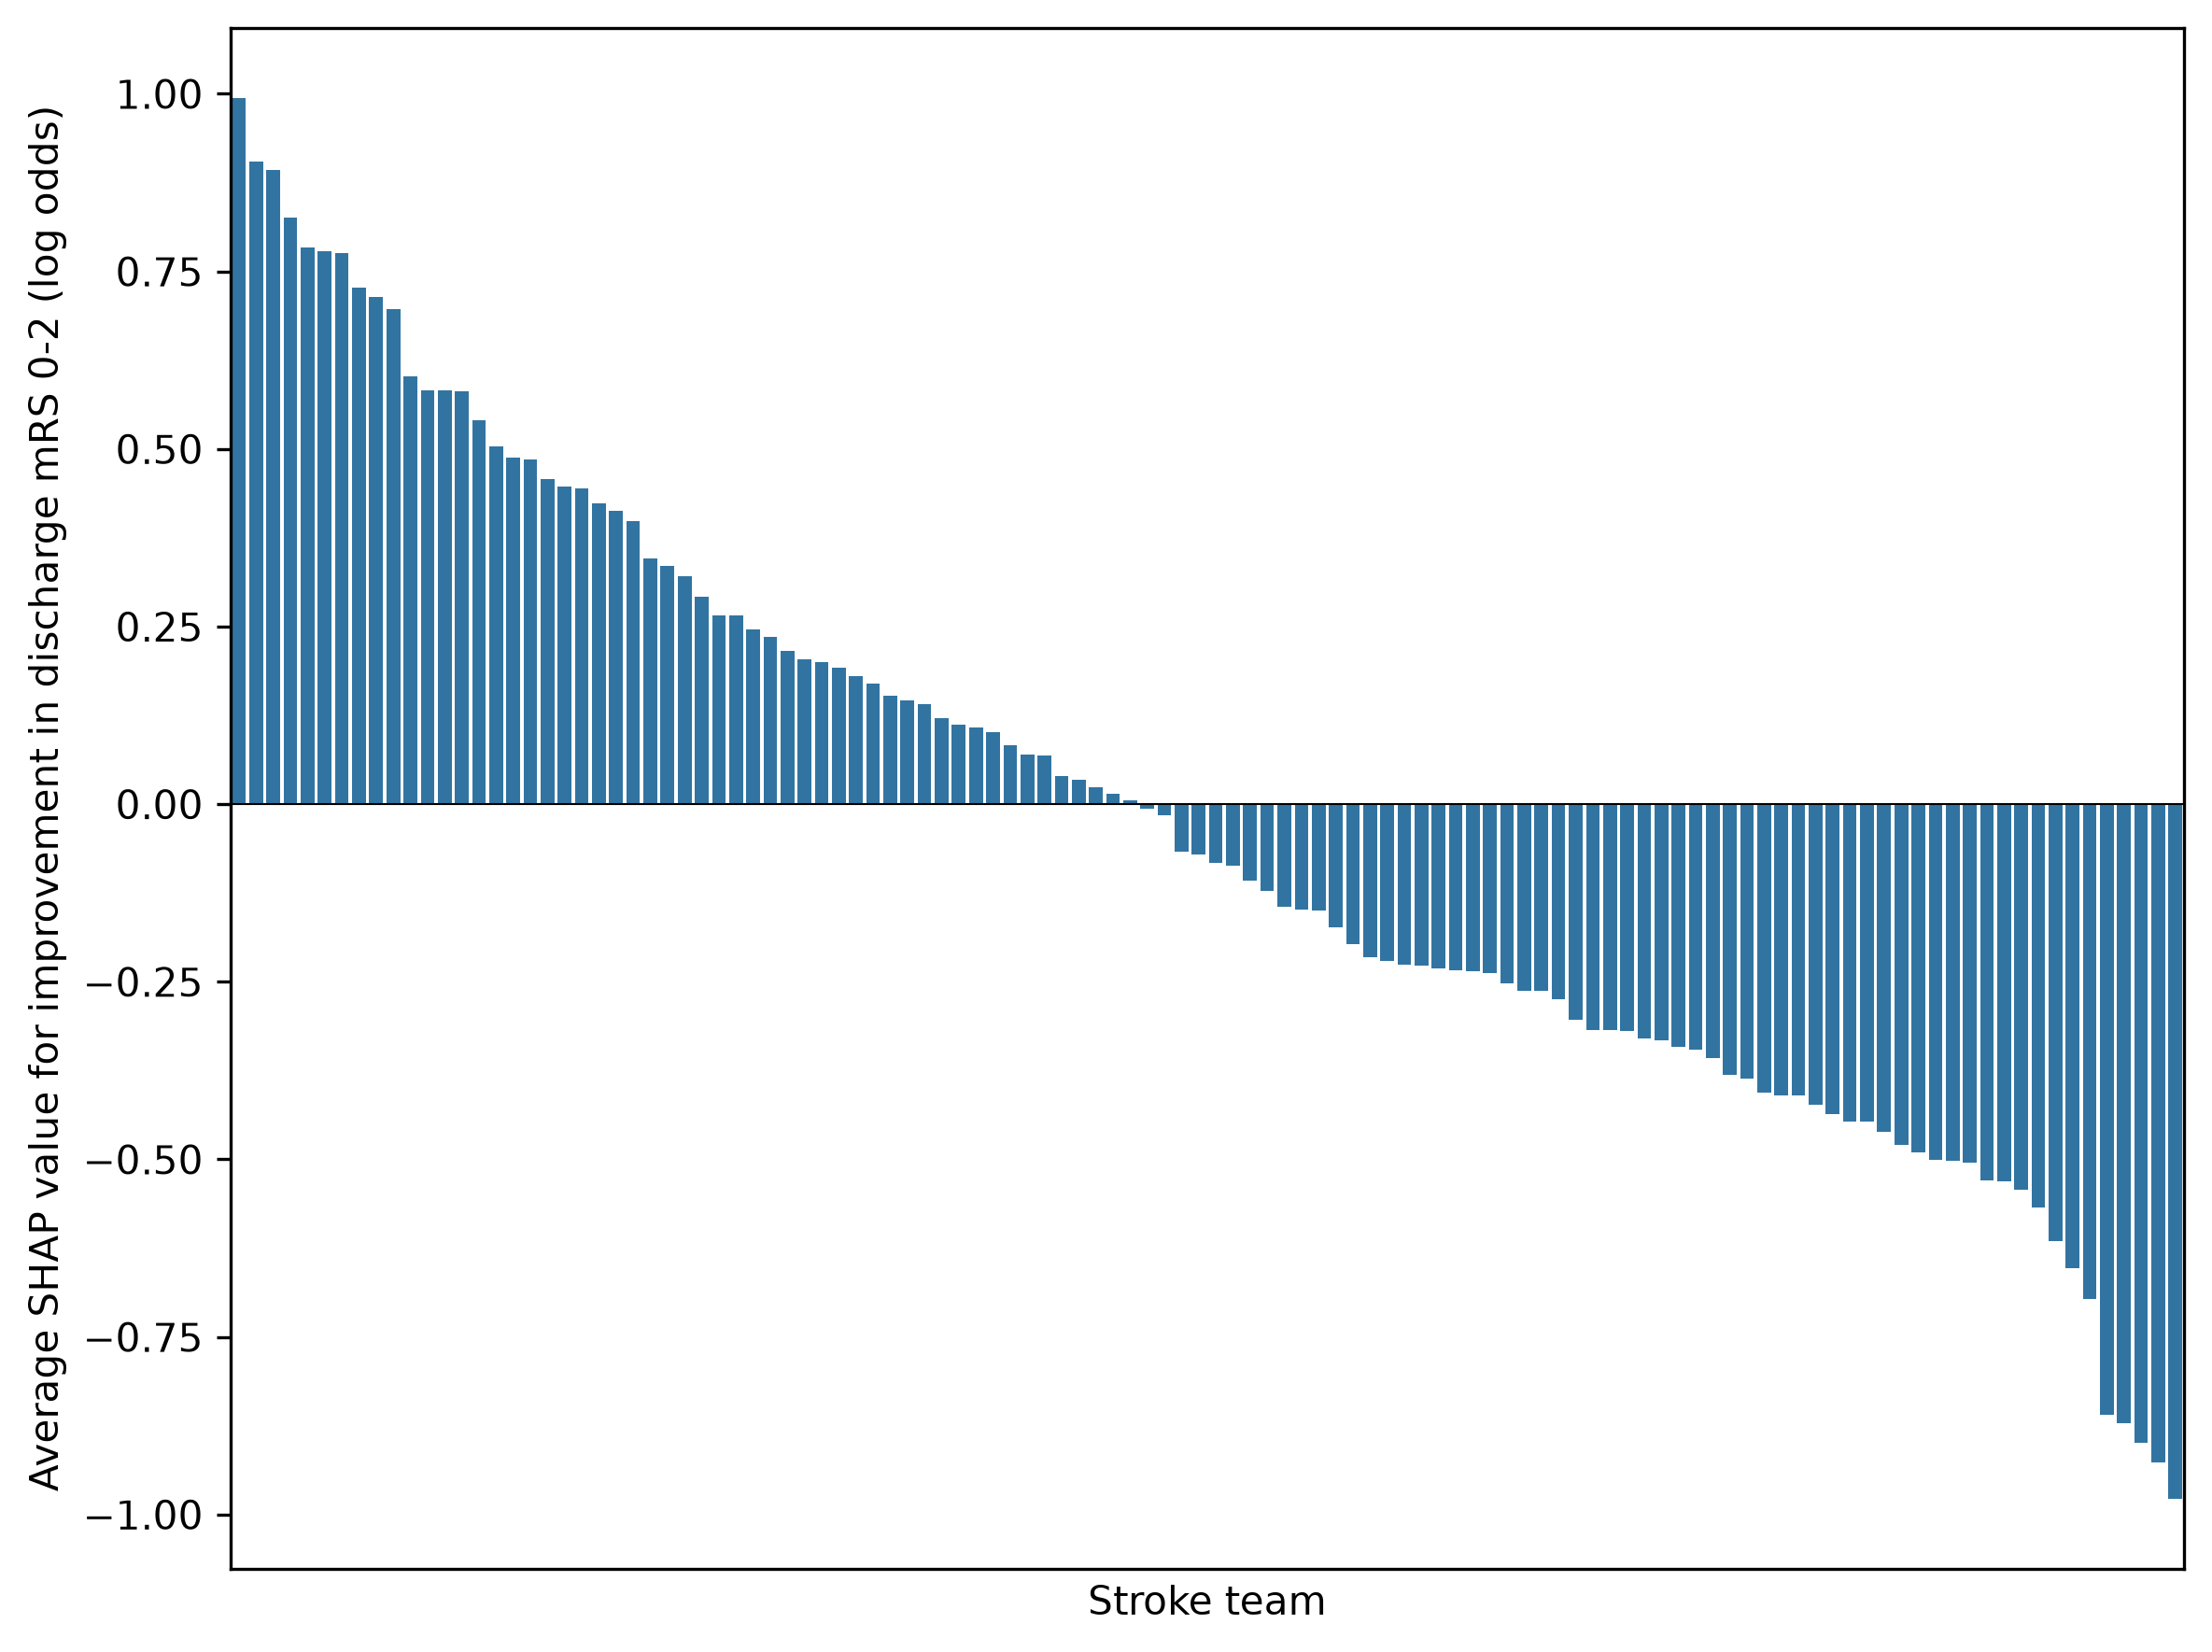
\includegraphics[width=\linewidth]{images/shap/shap_untreated_patients_mrs_less_than_3_stroke_team.png}
        %\caption{}
        \label{fig:bottom-right}
    \end{subfigure}

    \caption{SHAP analysis of feature contributions to predicting favourable discharge outcomes (mRS 0-2) in stroke patients who did not receive thrombolysis or thrombectomy. \textit{Top}: A SHAP summary plot detailing the impact of features on the model's log-odds predictions. Each point represents an individual patient instance. The position on the x-axis indicates the SHAP value, where positive values increase the predicted odds of a favourable outcome, and negative values decrease it. For continuous and binary variables, colour represents the original feature value (red indicating high values; blue indicating low values). Categorical variables (\textit{stroke team} and \textit{ethnicity}) are plotted in grey. \textit{Bottom left}: Violin plots illustrating the distribution of SHAP values across distinct ethnic groups. This panel highlights the marginal impact and variance of ethnicity on the model’s prediction for disability outcome. \textit{Bottom Right}: A ranked bar chart displaying the average SHAP value associated with each individual stroke team. This panel visualizes institutional variation, reflecting the contribution of the treating stroke team to the predicted patient outcome after accounting for patient-level clinical characteristics.}
    \label{fig:shap_mrs0-2_no_treatment}
\end{figure}

%%%%%%%%%%% Survival %%%%%%%%%%%%%%%

%% All patients

\begin{figure}[htbp]
    \centering
    
    % Top image (Full width)
    \begin{subfigure}{0.50\textwidth}
        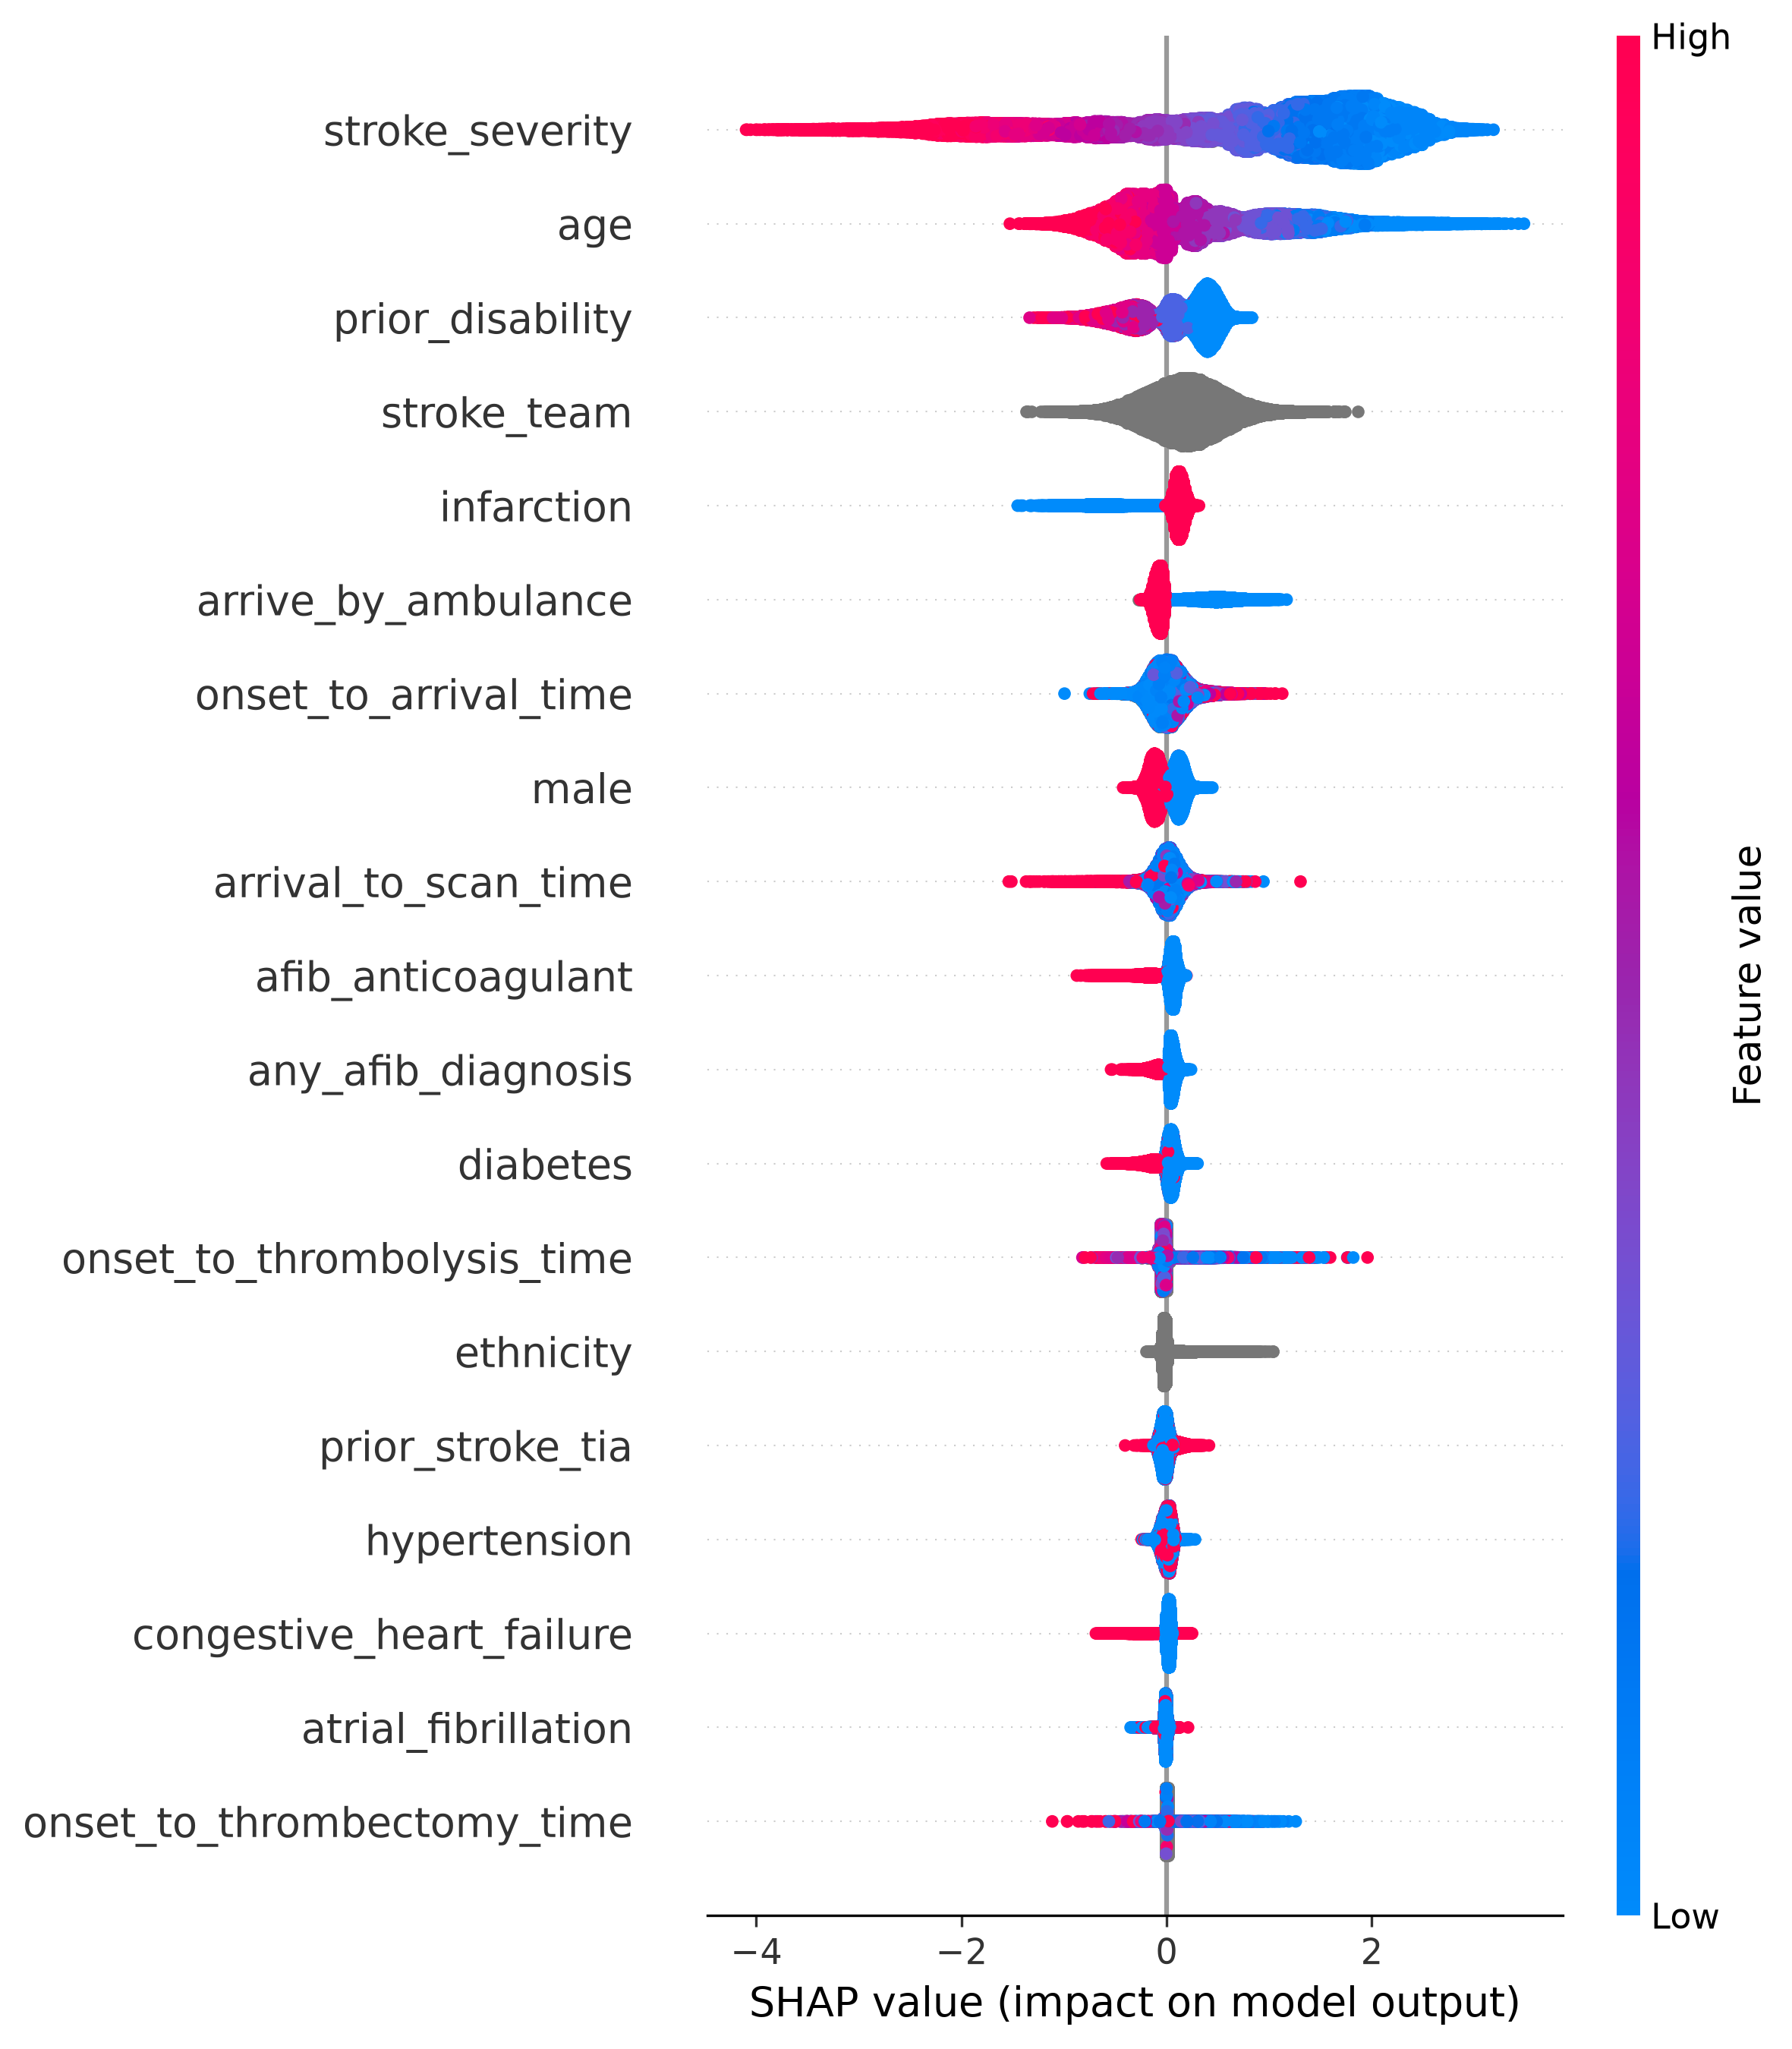
\includegraphics[width=\linewidth]{images/shap/shap_all_patients_survival.png}
        %\caption{}
        \label{fig:top}
    \end{subfigure}

    \vspace{0.5cm} % Optional vertical space between rows

    % Bottom left image (~45% width)
    \begin{subfigure}{0.407\textwidth}
        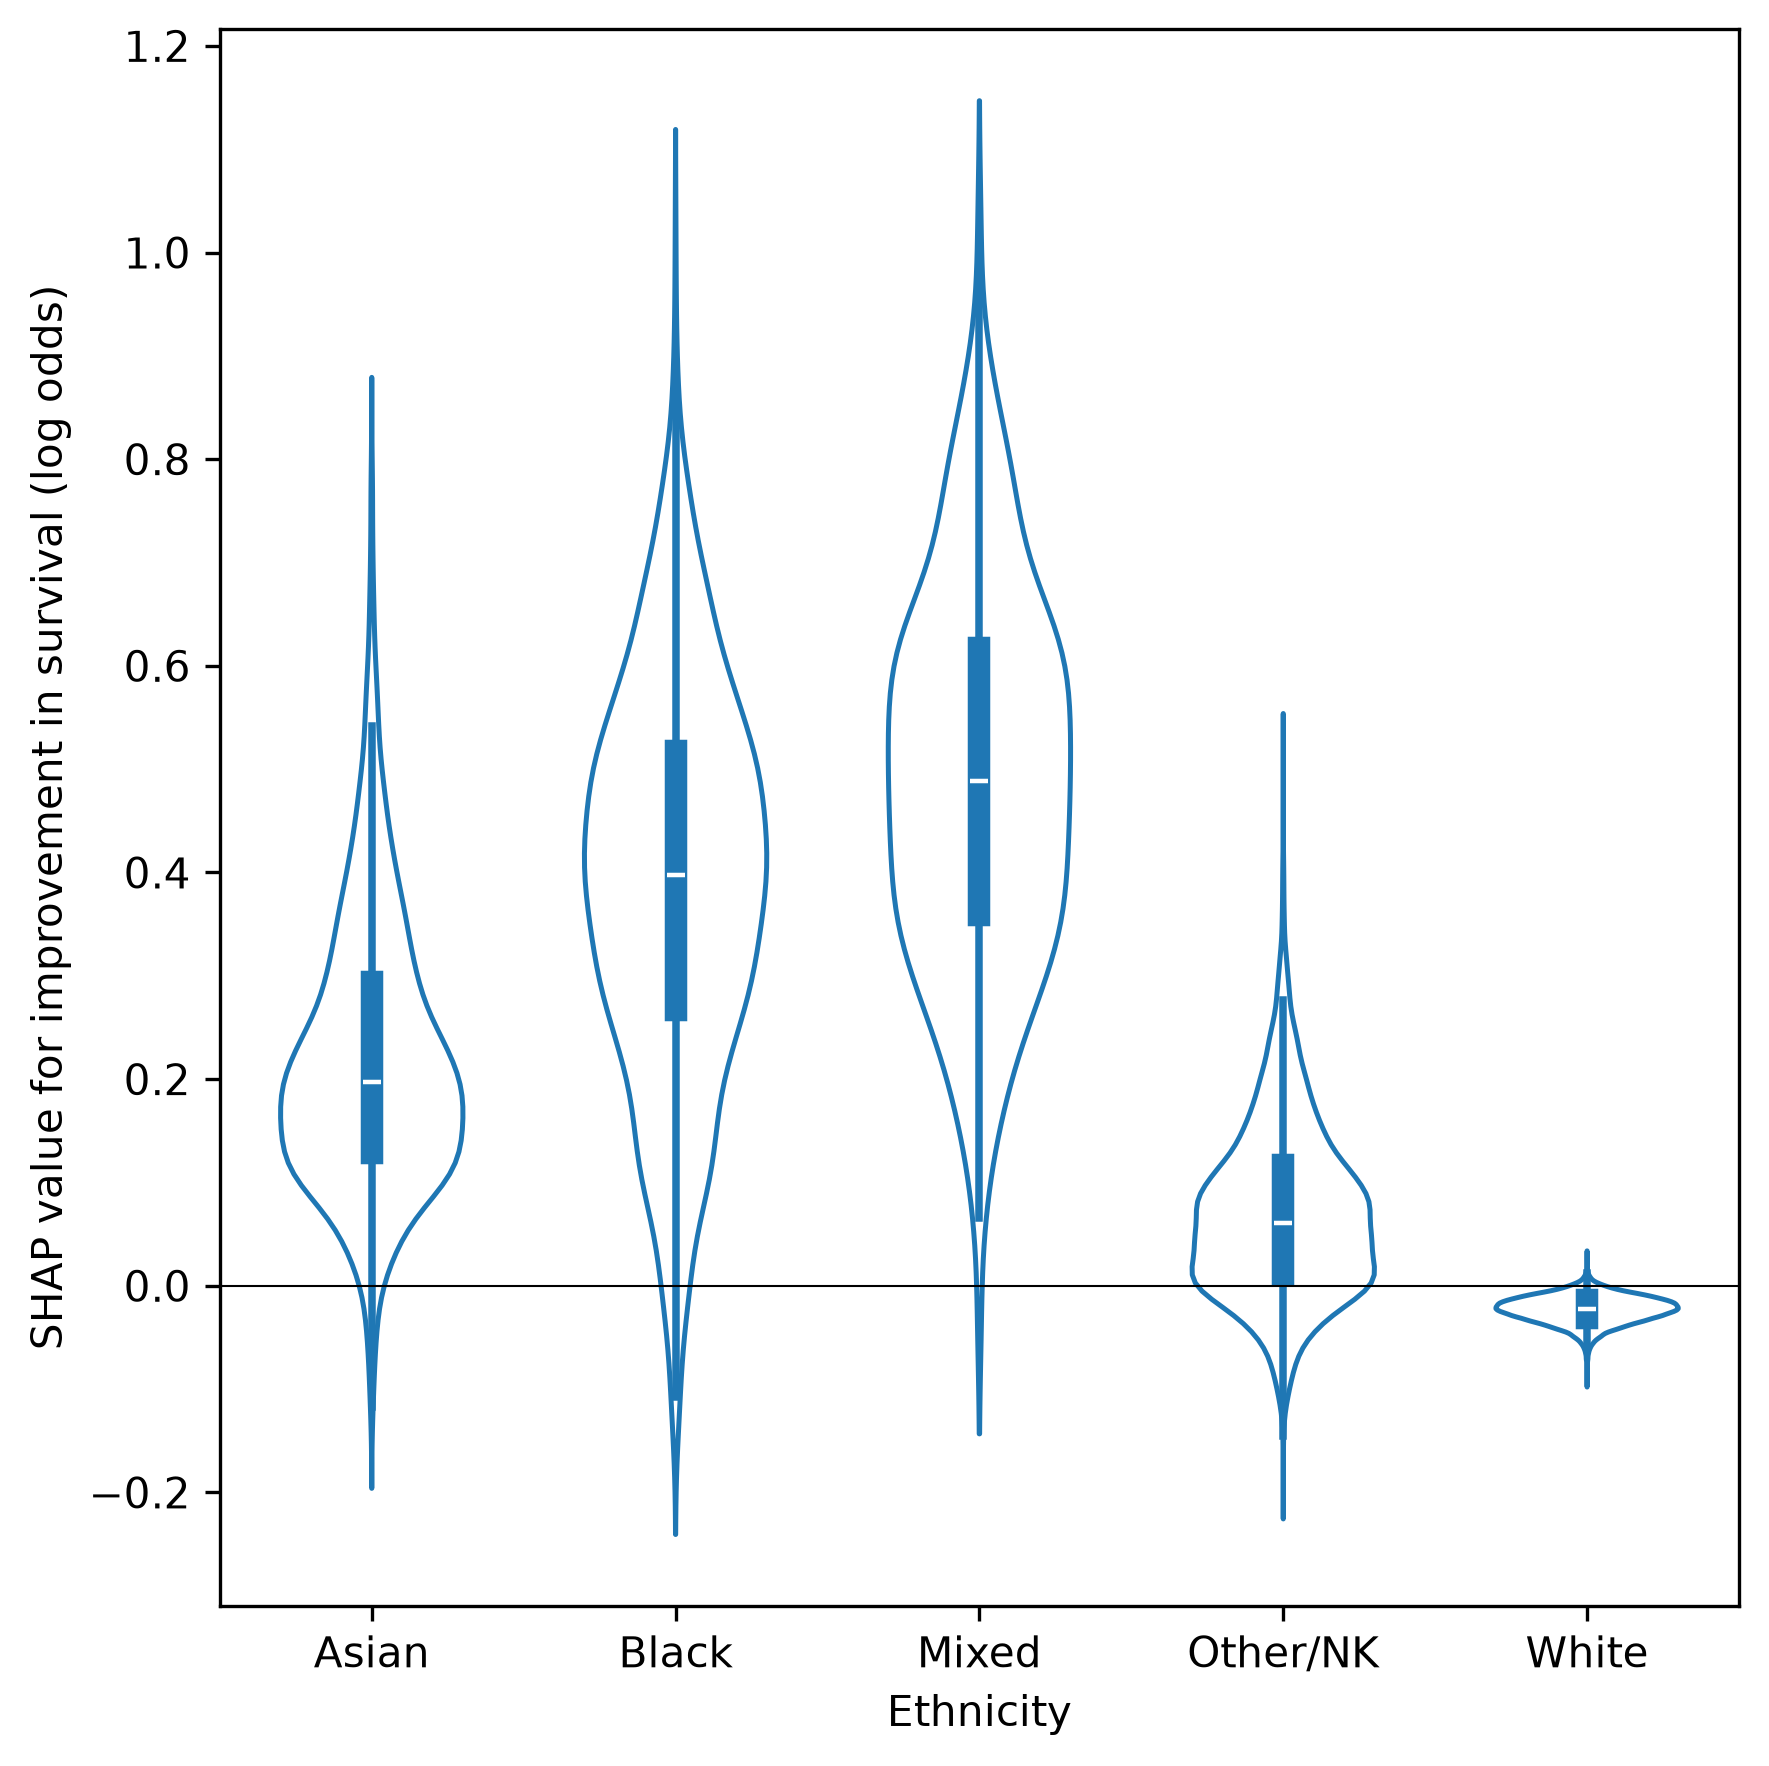
\includegraphics[width=\linewidth]{images/shap/shap_all_patients_survival_ethnicity.png}
        %\caption{}
        \label{fig:bottom-left}
    \end{subfigure}
    \hfill % Adds flexible horizontal spacing
    % Bottom right image (~55% width)
    \begin{subfigure}{0.543\textwidth}
        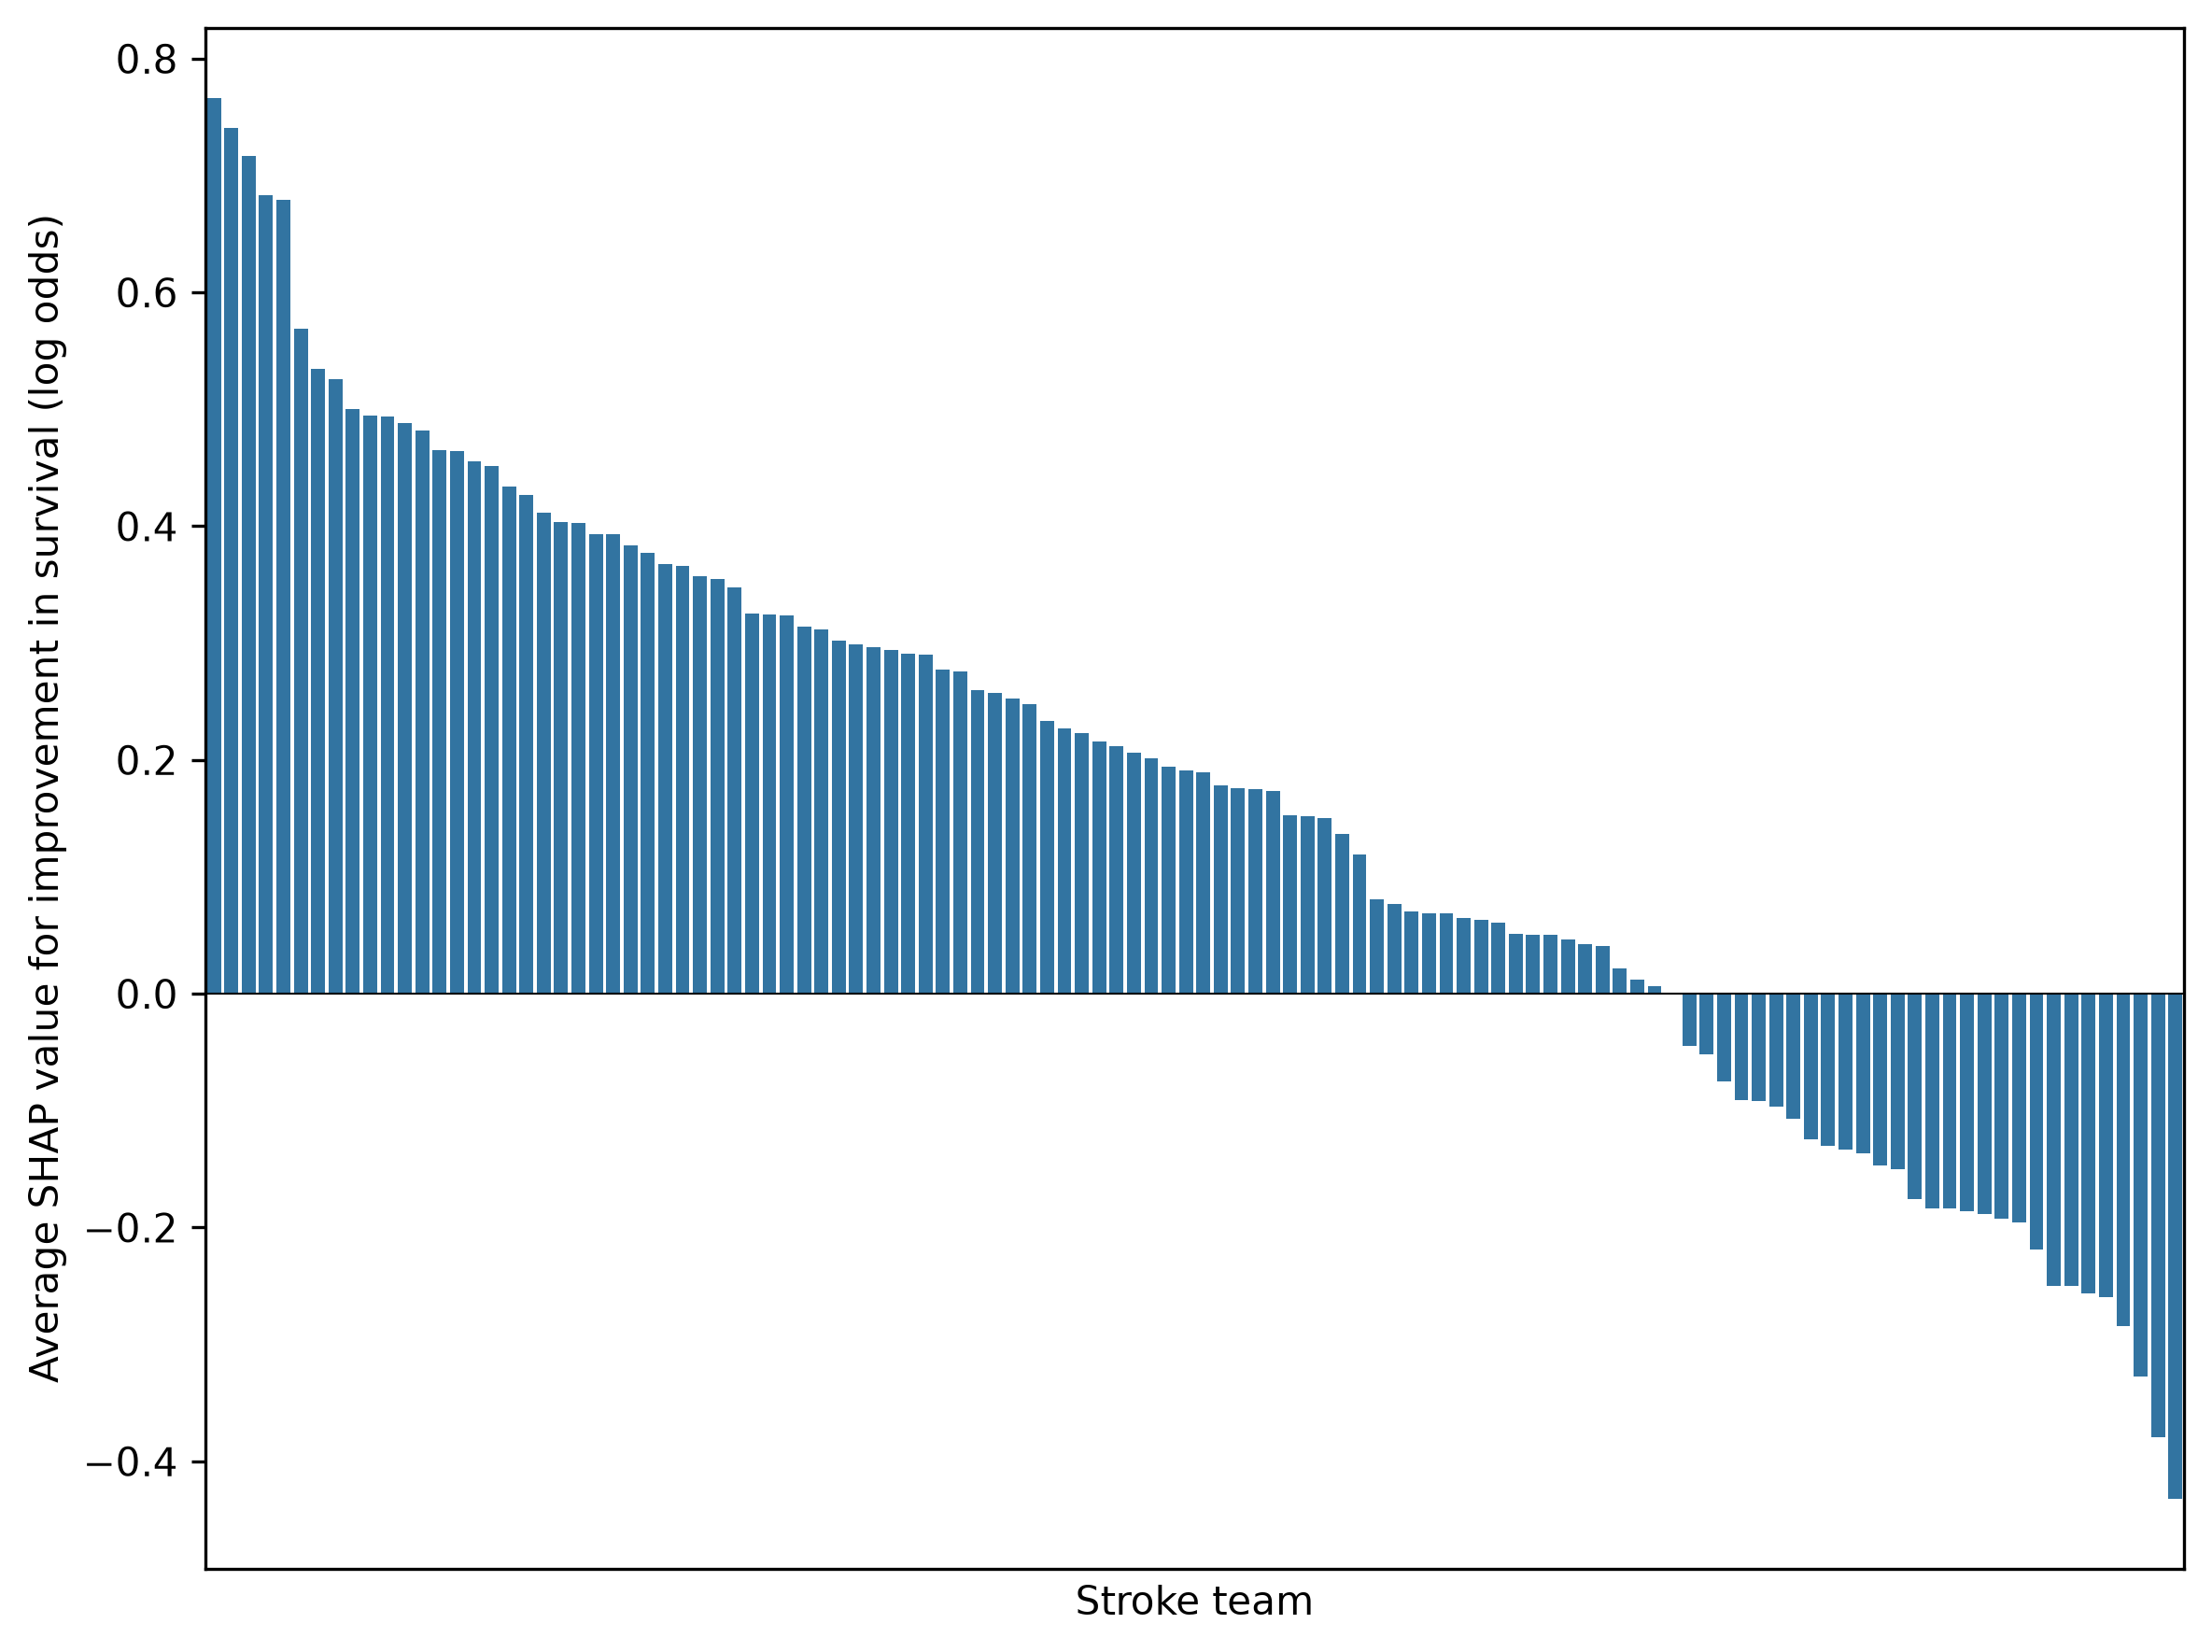
\includegraphics[width=\linewidth]{images/shap/shap_all_patients_survival_stroke_team.png}
        %\caption{}
        \label{fig:bottom-right}
    \end{subfigure}

    \caption{SHAP analysis of feature contributions to predicting survival in stroke patients. \textit{Top}: A SHAP summary plot detailing the impact of features on the model's log-odds predictions. Each point represents an individual patient instance. The position on the x-axis indicates the SHAP value, where positive values increase the predicted odds of survival, and negative values decrease it. For continuous and binary variables, colour represents the original feature value (red indicating high values; blue indicating low values). Categorical variables (\textit{stroke team} and \textit{ethnicity}) are plotted in grey. \textit{Bottom left}: Violin plots illustrating the distribution of SHAP values across distinct ethnic groups. This panel highlights the marginal impact and variance of ethnicity on the model’s prediction for survival. \textit{Bottom Right}: A ranked bar chart displaying the average SHAP value associated with each individual stroke team. This panel visualizes institutional variation, reflecting the contribution of the treating stroke team to the predicted survival outcome after accounting for patient-level clinical characteristics.}
    \label{fig:shap_survival_all}
\end{figure}

%% Untreated patients

\begin{figure}[htbp]
    \centering
    
    % Top image (Full width)
    \begin{subfigure}{0.50\textwidth}
        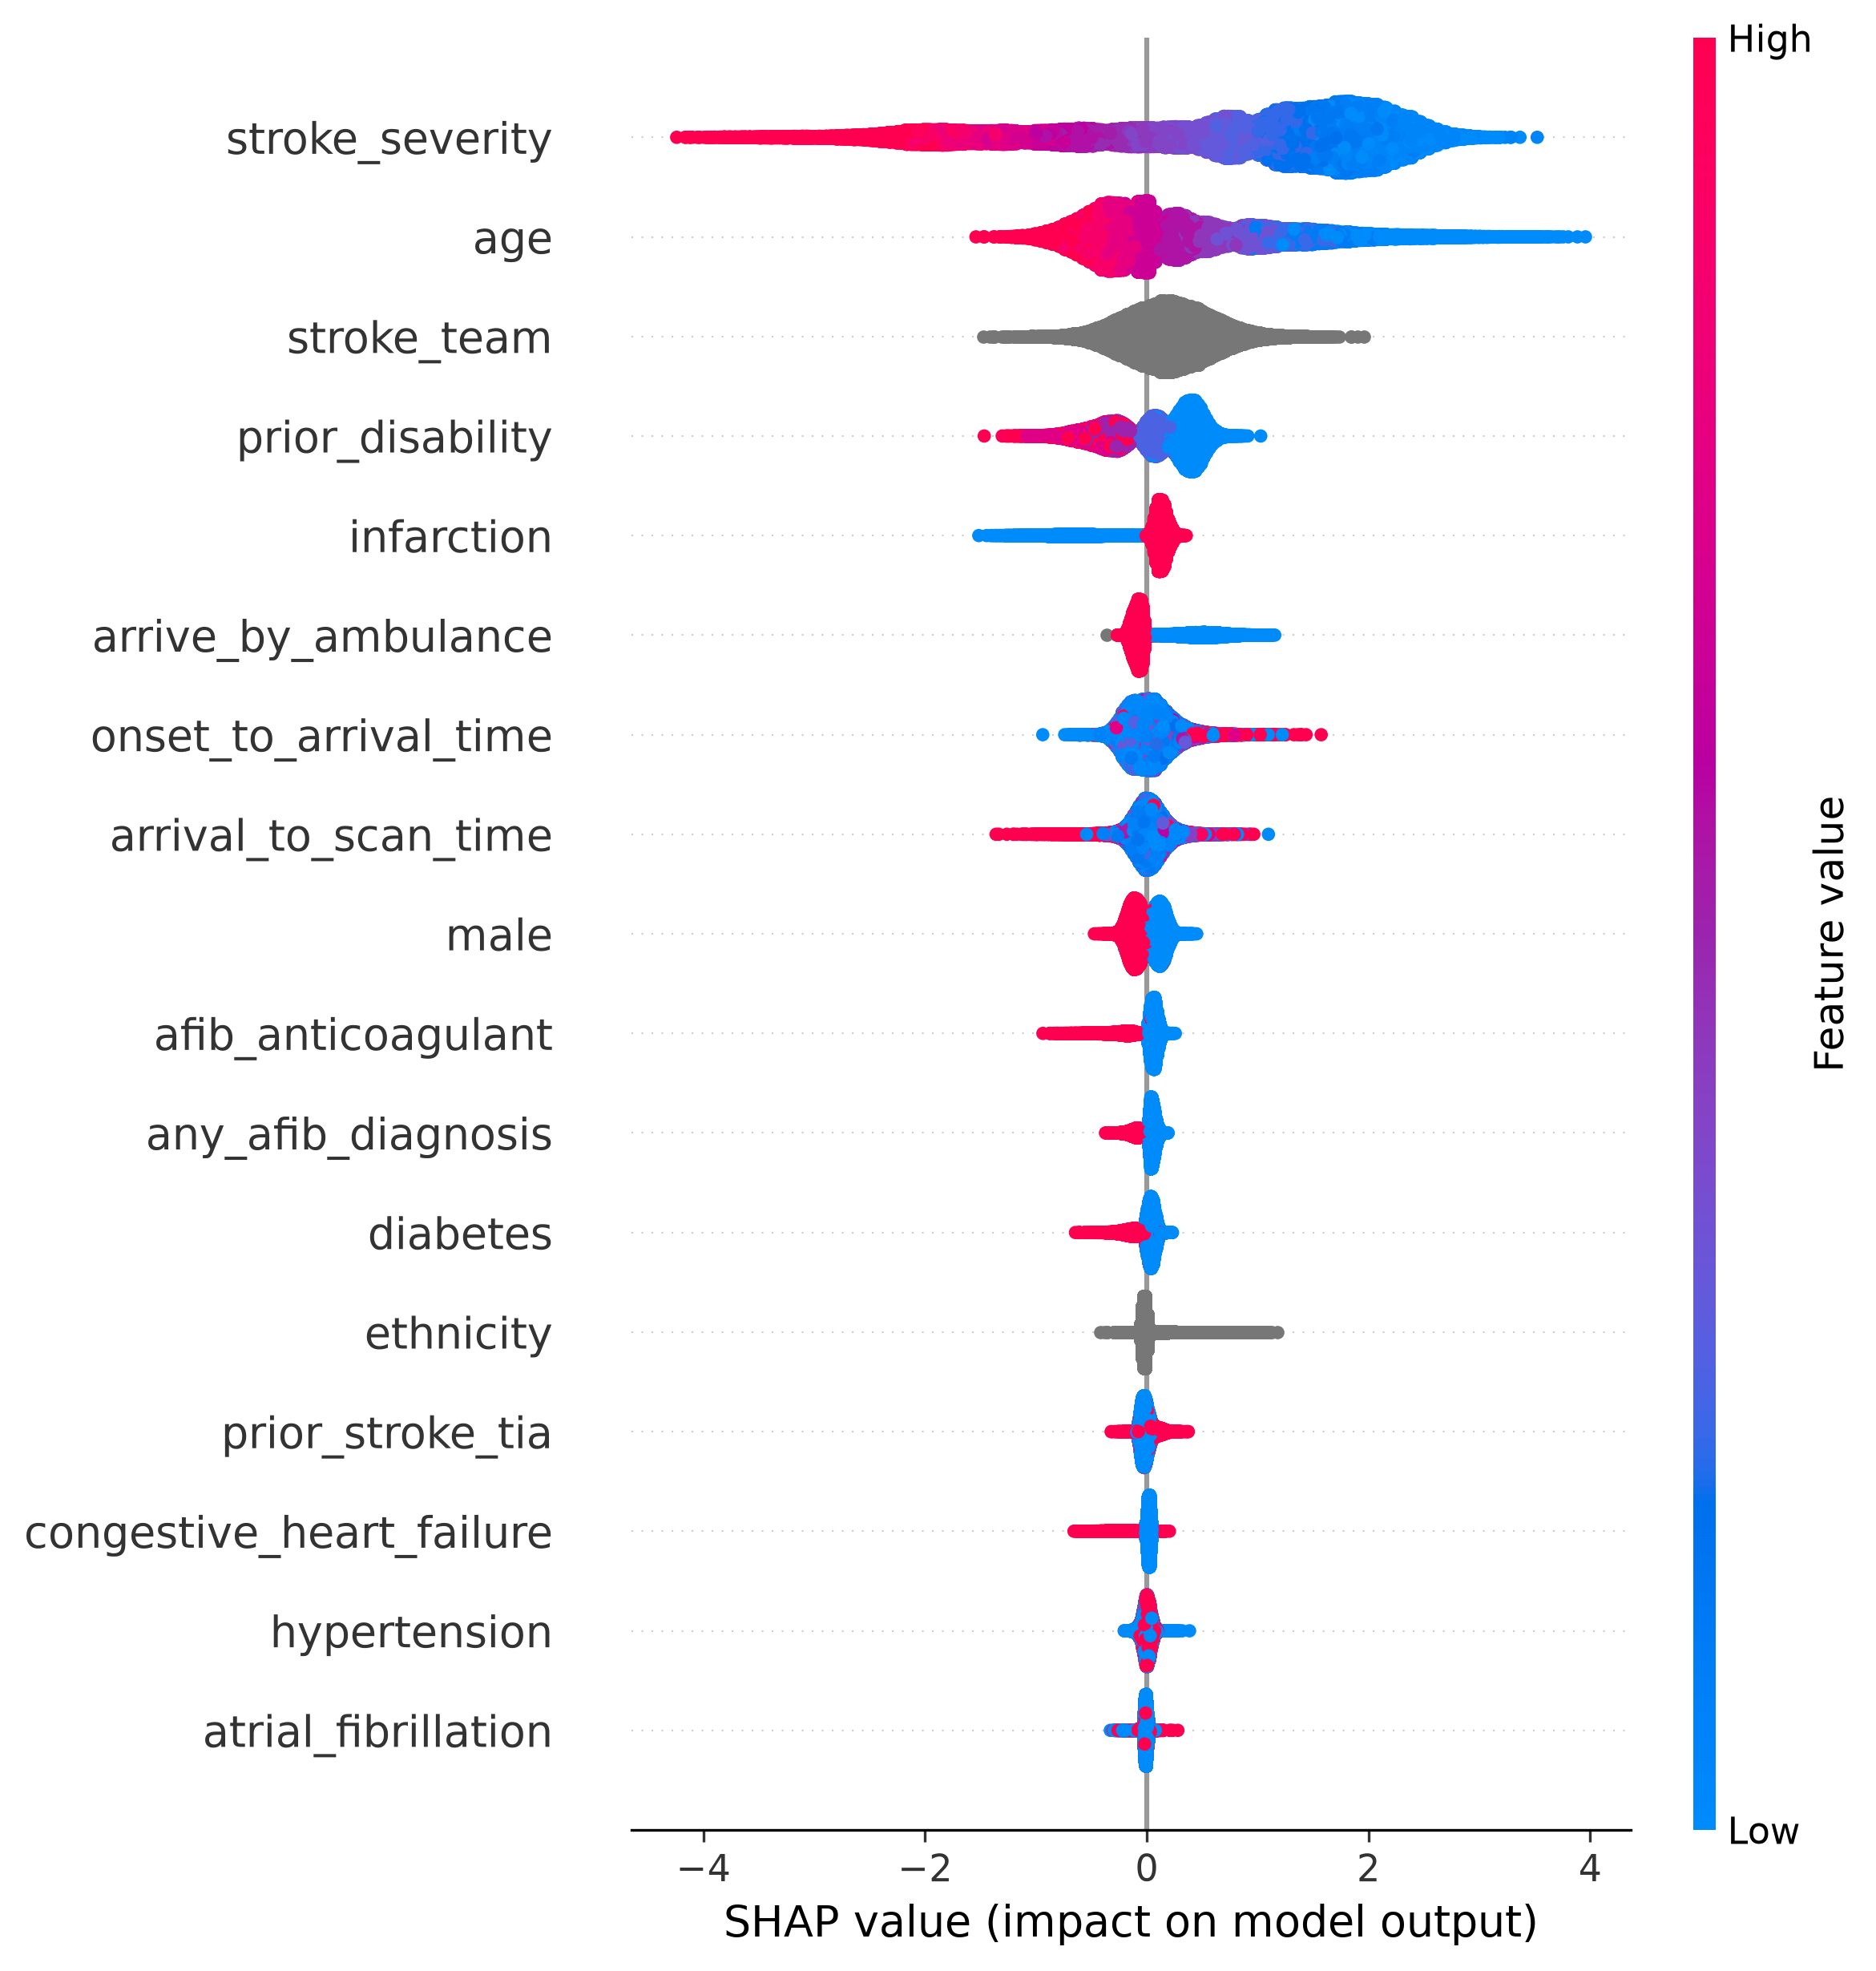
\includegraphics[width=\linewidth]{images/shap/shap_untreated_patients_survival.png}
        %\caption{}
        \label{fig:top}
    \end{subfigure}

    \vspace{0.5cm} % Optional vertical space between rows

    % Bottom left image (~45% width)
    \begin{subfigure}{0.407\textwidth}
        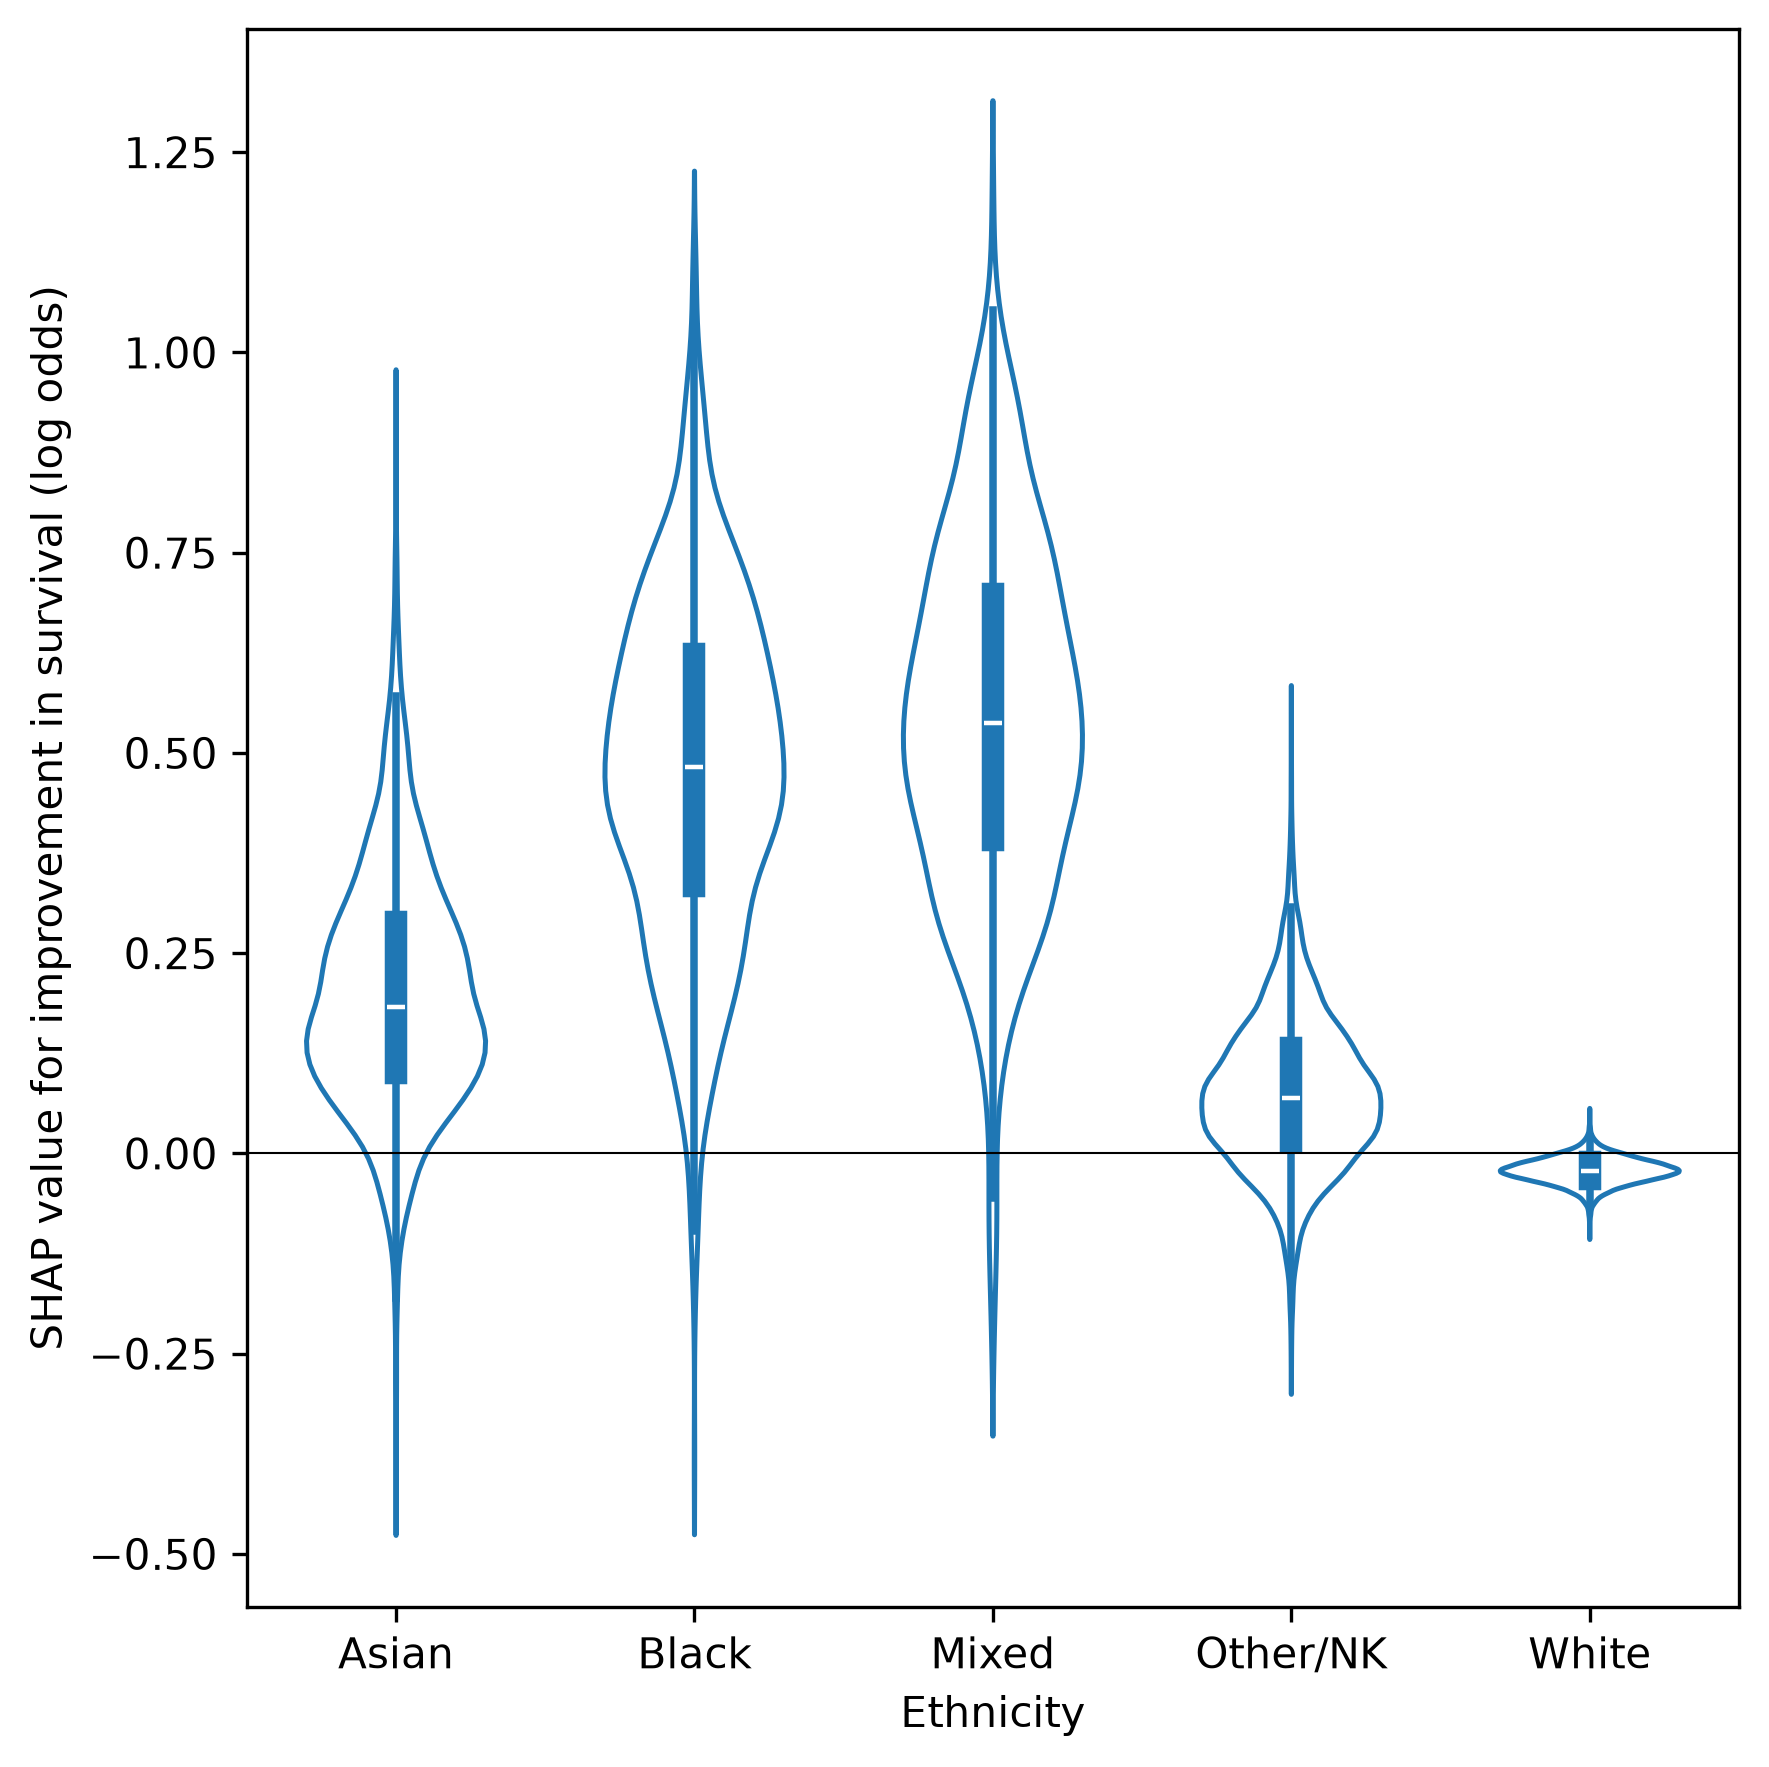
\includegraphics[width=\linewidth]{images/shap/shap_untreated_patients_survival_ethnicity.png}
        %\caption{}
        \label{fig:bottom-left}
    \end{subfigure}
    \hfill % Adds flexible horizontal spacing
    % Bottom right image (~55% width)
    \begin{subfigure}{0.543\textwidth}
        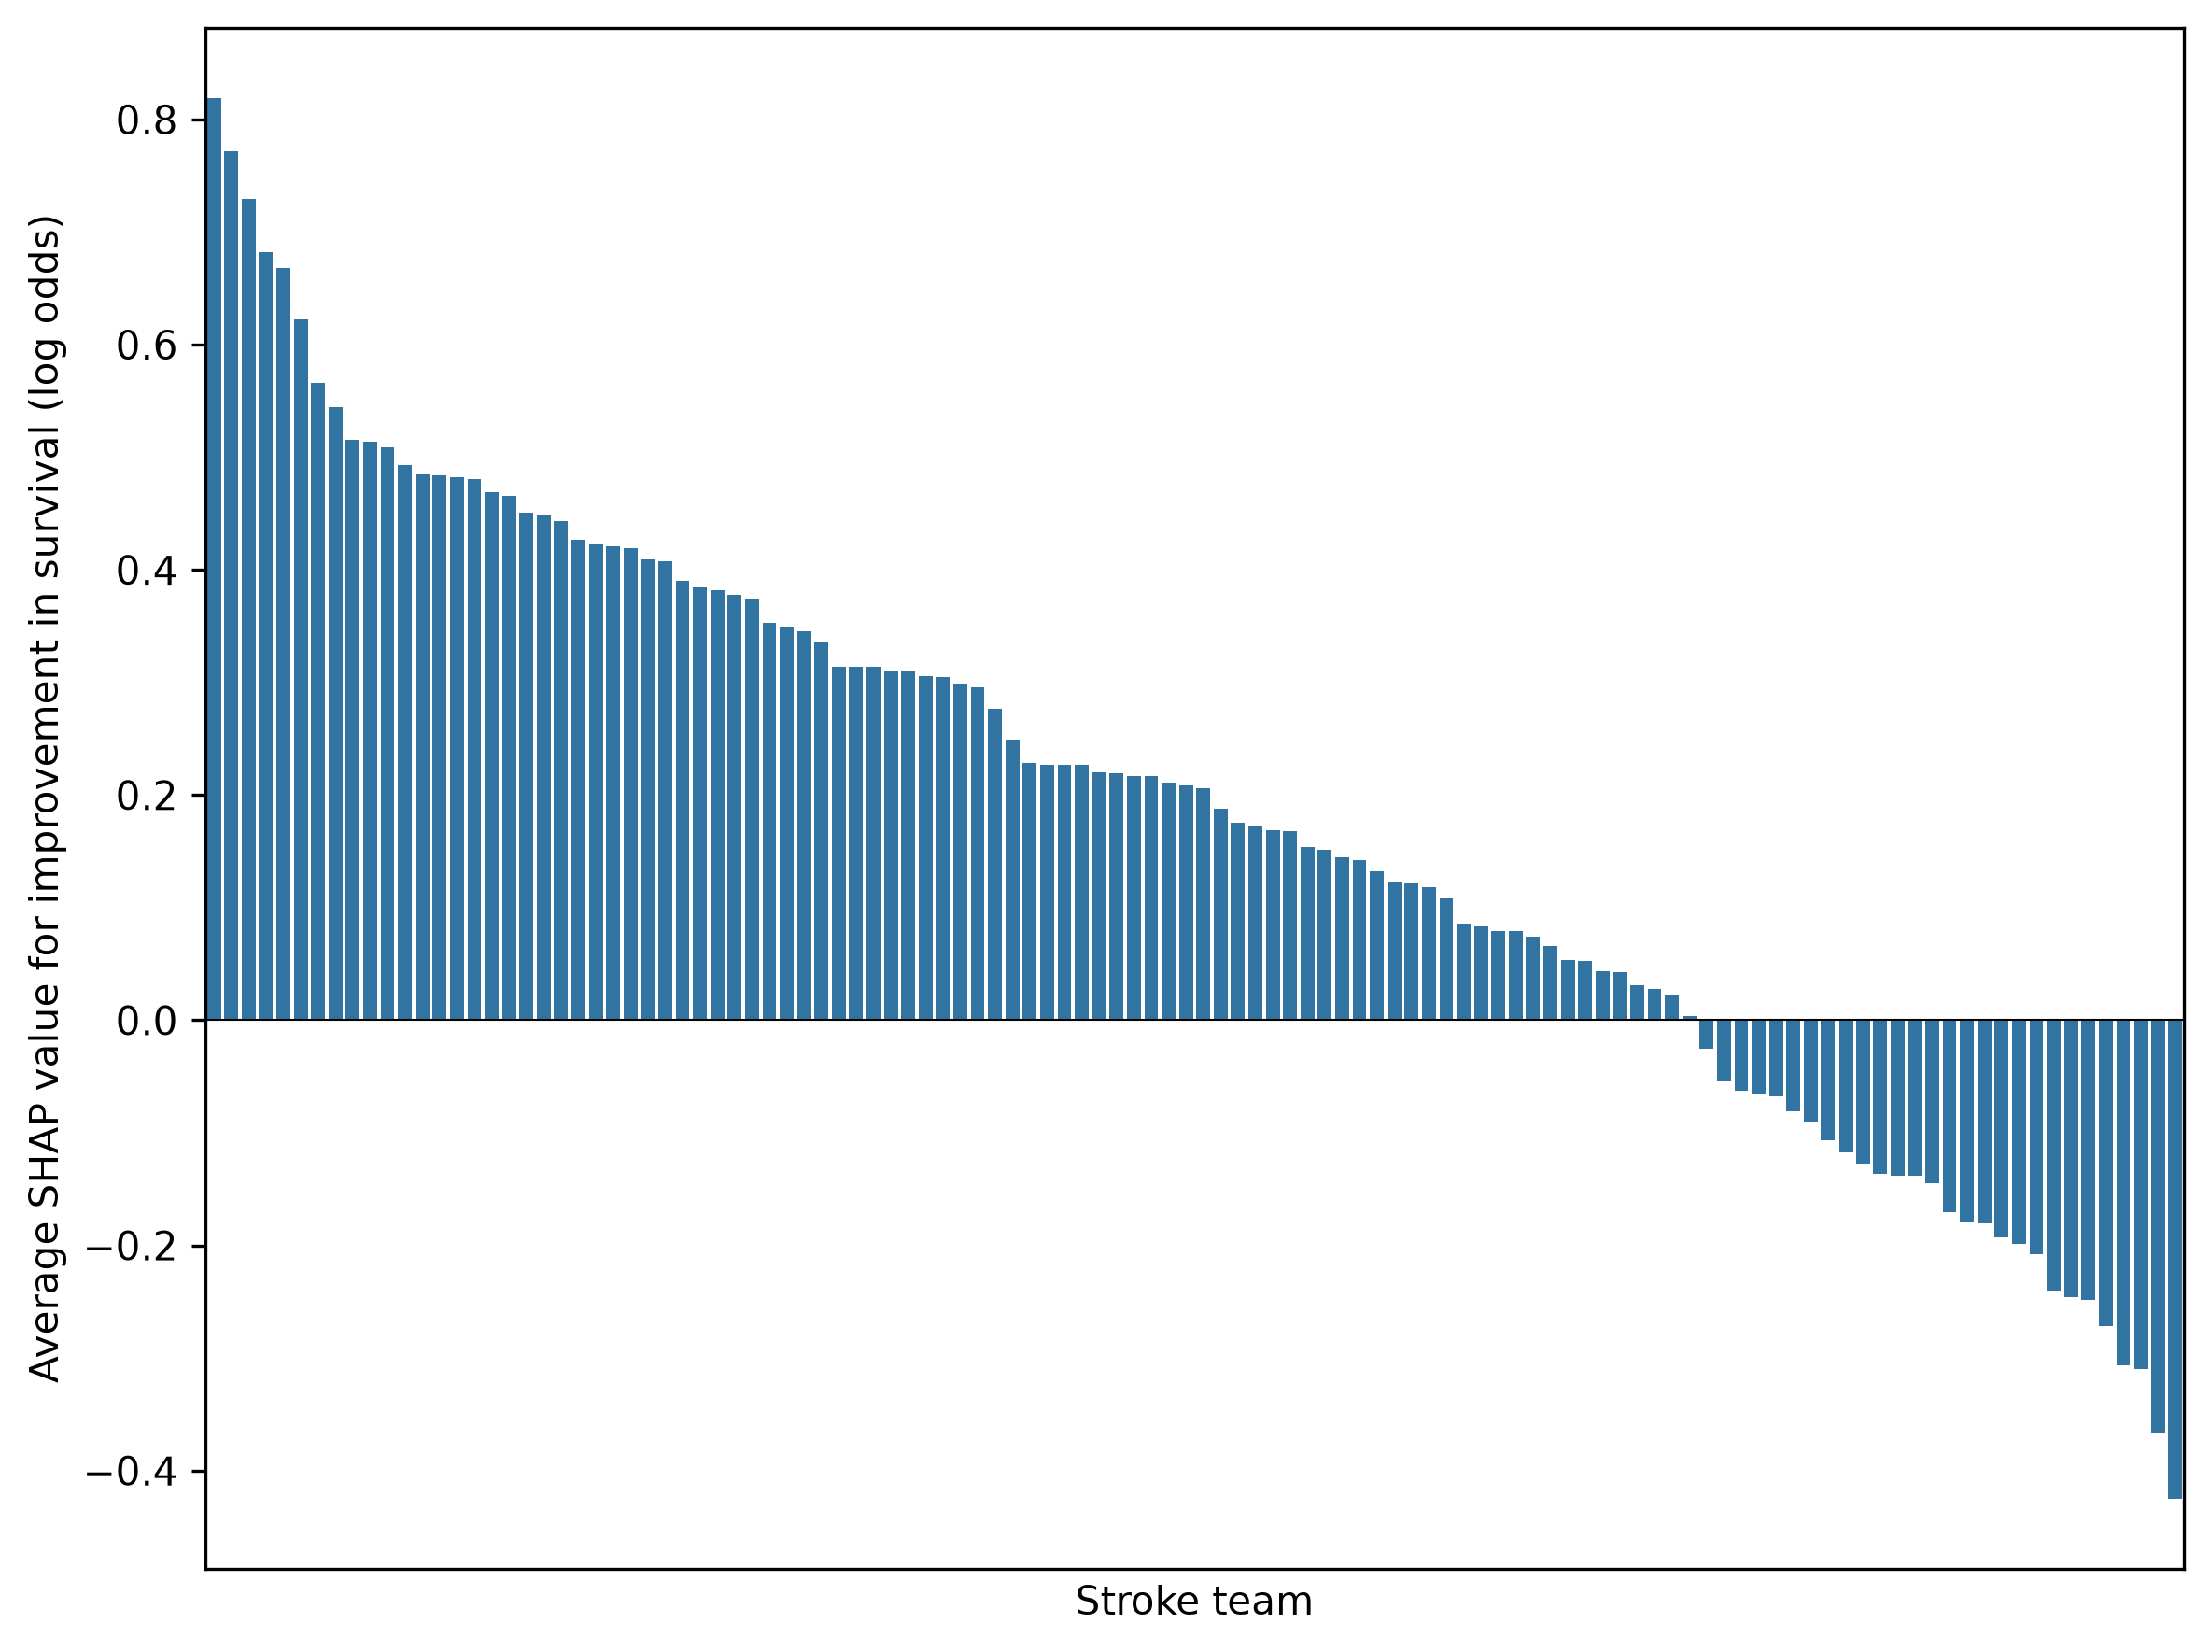
\includegraphics[width=\linewidth]{images/shap/shap_untreated_patients_survival_stroke_team.png}
        %\caption{}
        \label{fig:bottom-right}
    \end{subfigure}

    \caption{SHAP analysis of feature contributions to predicting survival in stroke patients who did not receive thrombolysis or thrombectomy. \textit{Top}: A SHAP summary plot detailing the impact of features on the model's log-odds predictions. Each point represents an individual patient instance. The position on the x-axis indicates the SHAP value, where positive values increase the predicted odds of survival, and negative values decrease it. For continuous and binary variables, colour represents the original feature value (red indicating high values; blue indicating low values). Categorical variables (\textit{stroke team} and \textit{ethnicity}) are plotted in grey. \textit{Bottom left}: Violin plots illustrating the distribution of SHAP values across distinct ethnic groups. This panel highlights the marginal impact and variance of ethnicity on the model’s prediction for survival. \textit{Bottom Right}: A ranked bar chart displaying the average SHAP value associated with each individual stroke team. This panel visualizes institutional variation, reflecting the contribution of the treating stroke team to the predicted survival outcome after accounting for patient-level clinical characteristics.}
    \label{fig:shap_survival_no_treatment}
\end{figure}

%%%%%%%%%%%%%%%%%%%%%%%%%% Length of stay %%%%%%%%%%%%%%%%%%%%%%%%%%%%%

%% All patients

\begin{figure}[htbp]
    \centering
    
    % Top image (Full width)
    \begin{subfigure}{0.50\textwidth}
        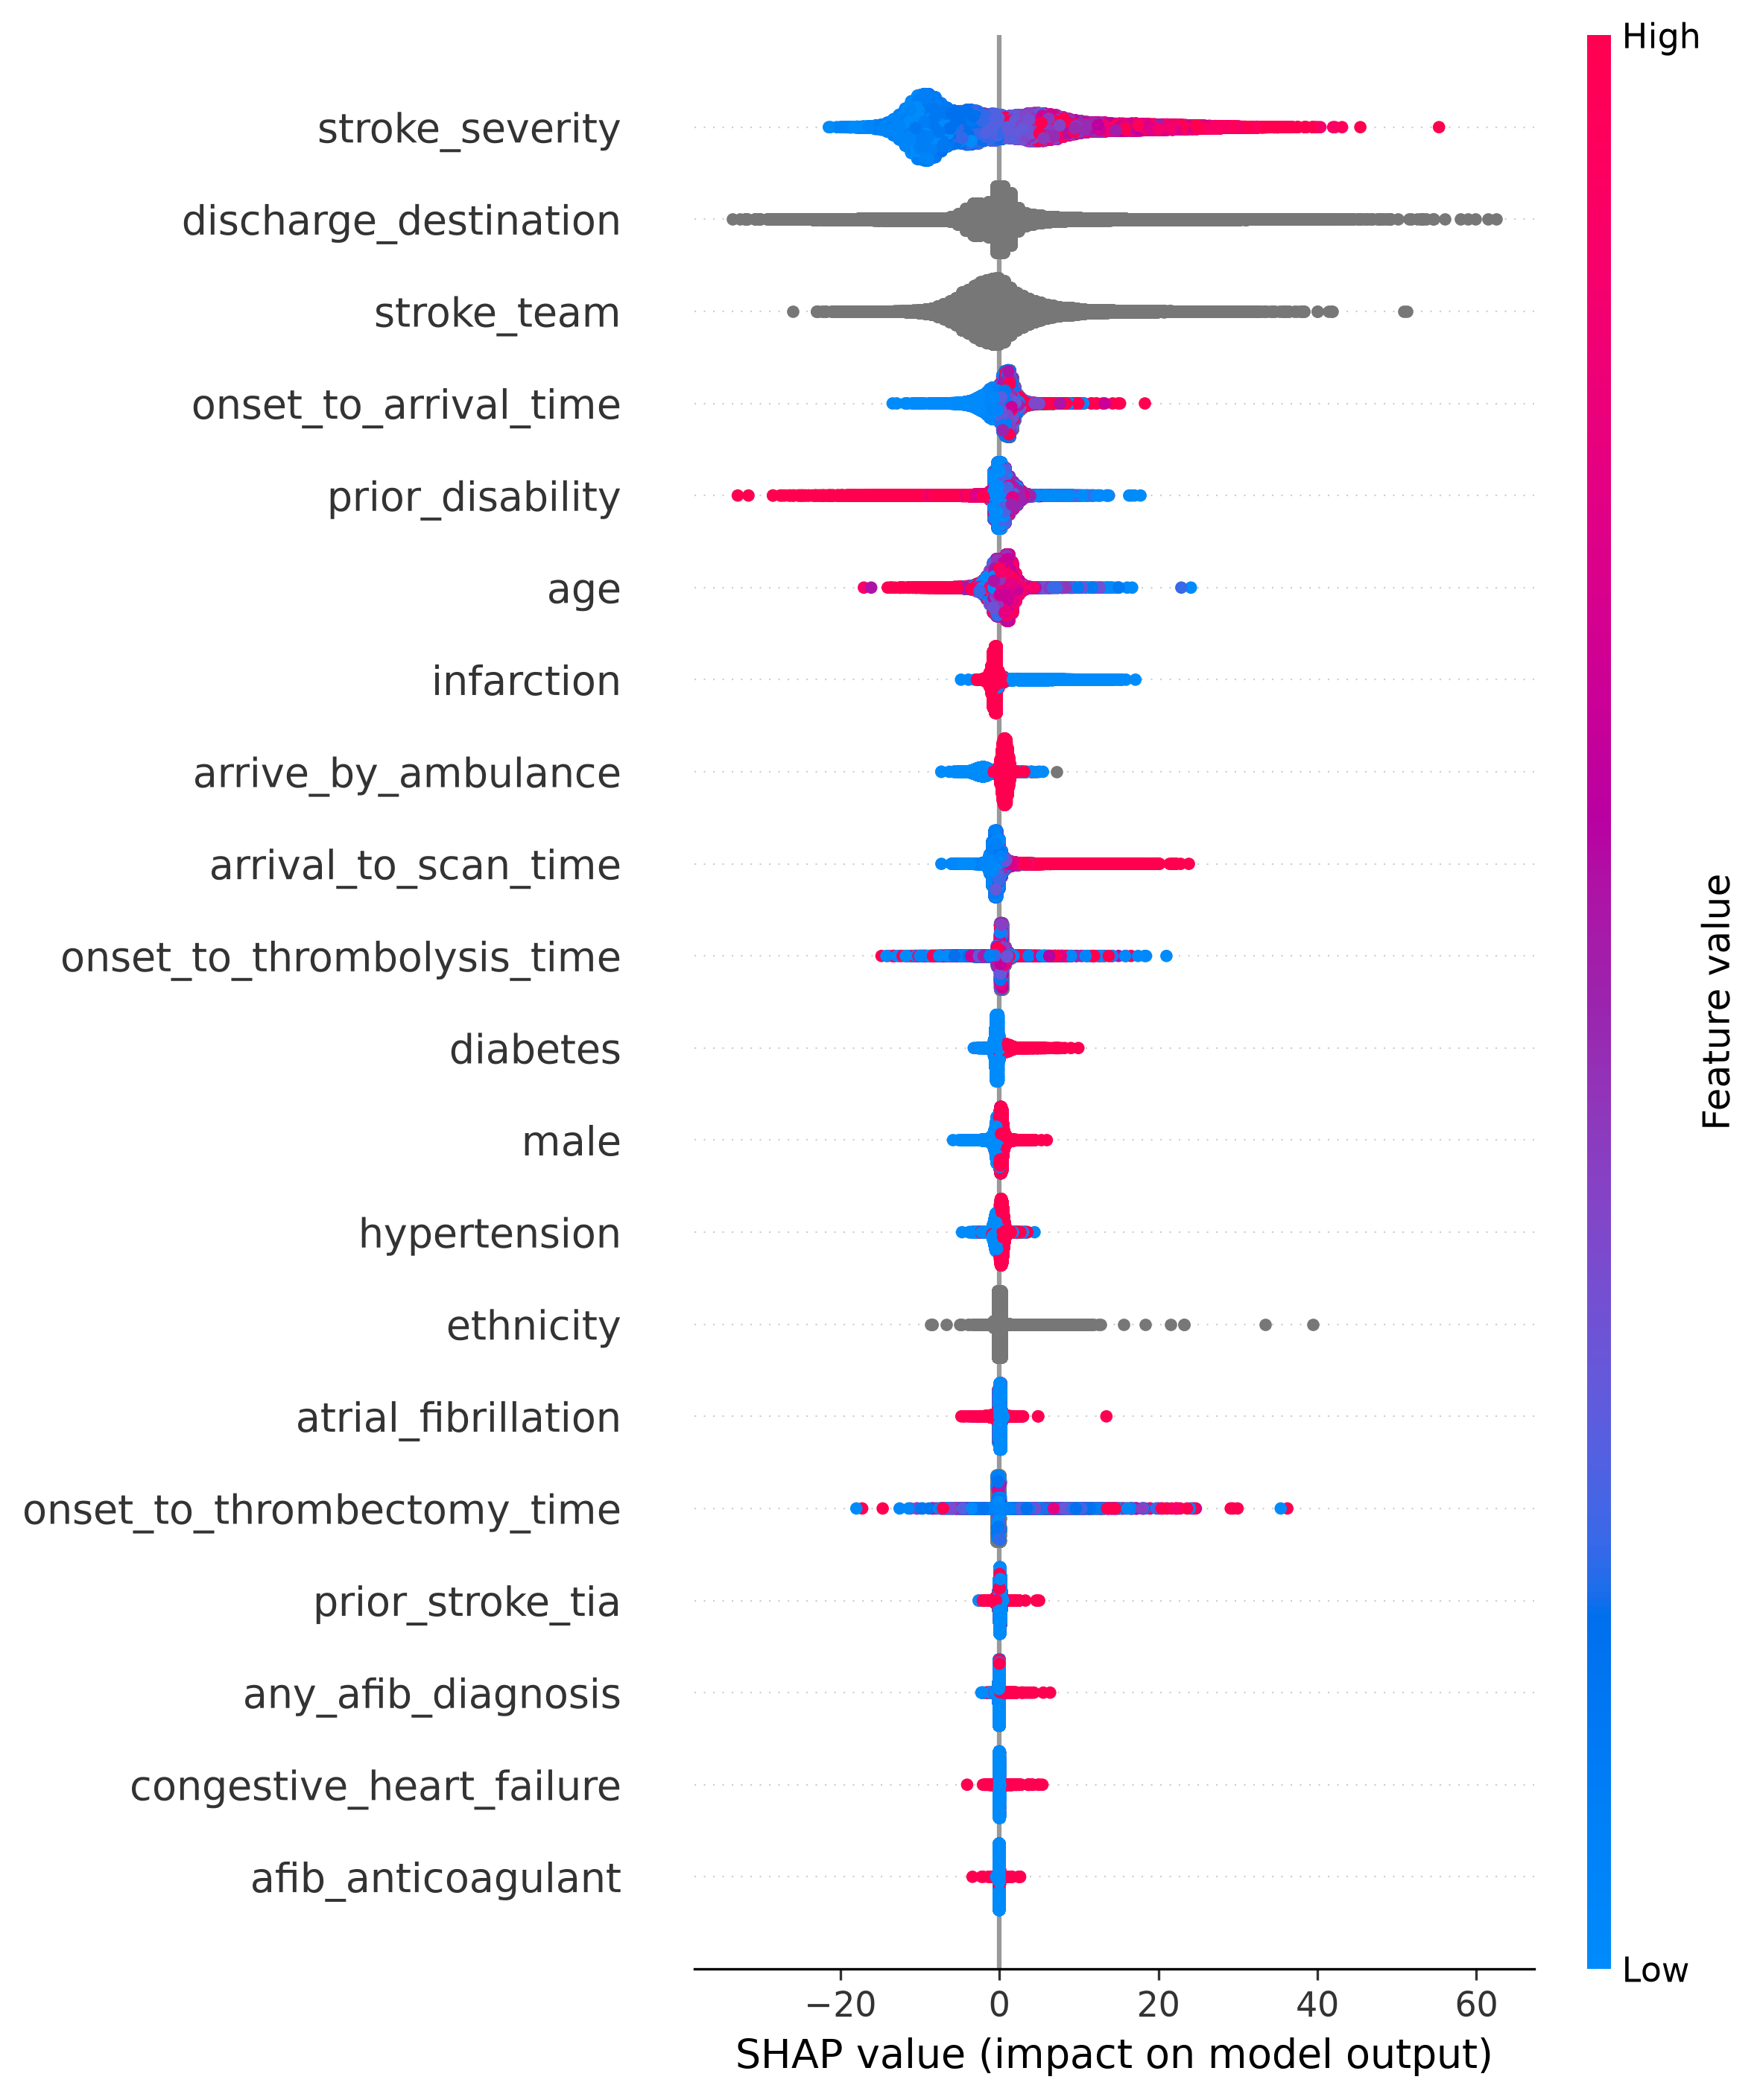
\includegraphics[width=\linewidth]{images/shap/shap_all_patients_los.png}
        %\caption{}
        \label{fig:top}
    \end{subfigure}

    \vspace{0.5cm} % Optional vertical space between rows

    % Bottom left image (~45% width)
    \begin{subfigure}{0.24\textwidth}
        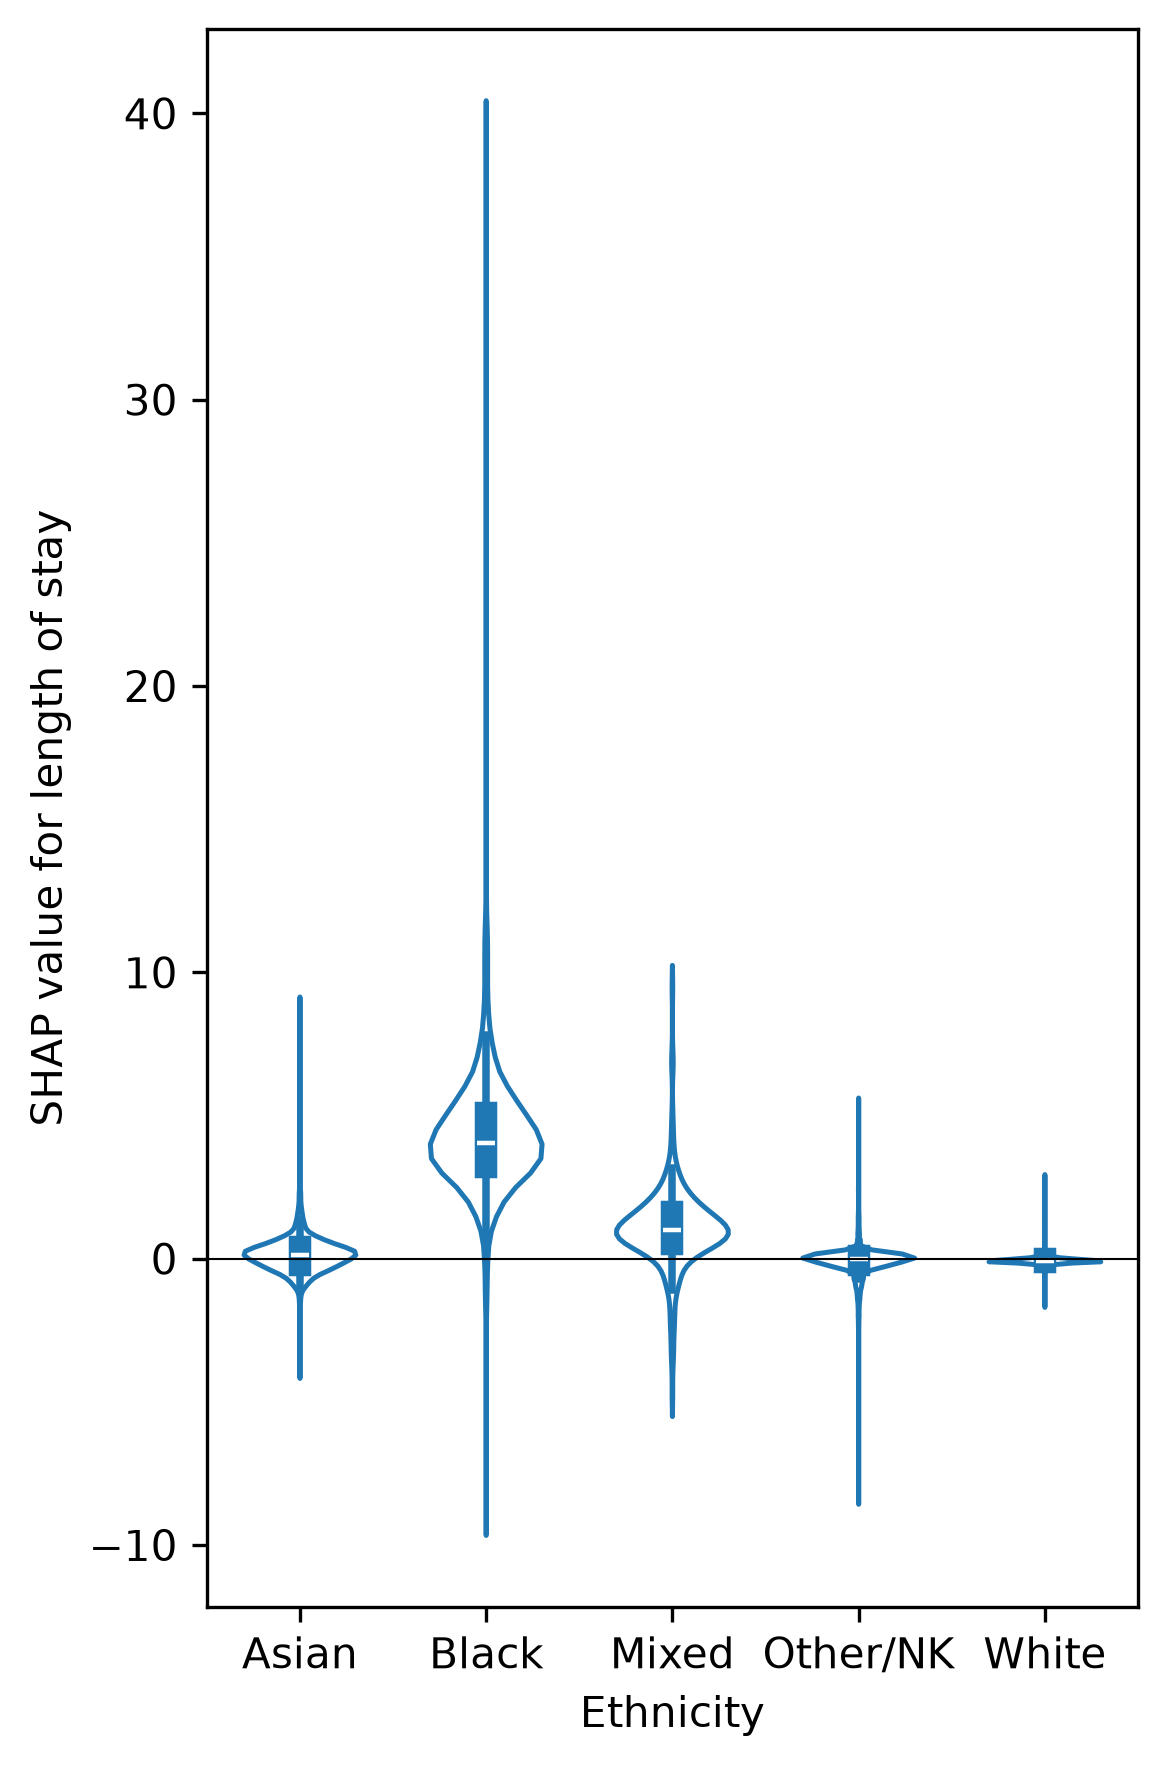
\includegraphics[width=\linewidth]{images/shap/shap_all_patients_los_ethnicity.png}
        %\caption{}
        \label{fig:bottom-left}
    \end{subfigure}
    \hfill % Adds flexible horizontal spacing
        \begin{subfigure}{0.24\textwidth}
        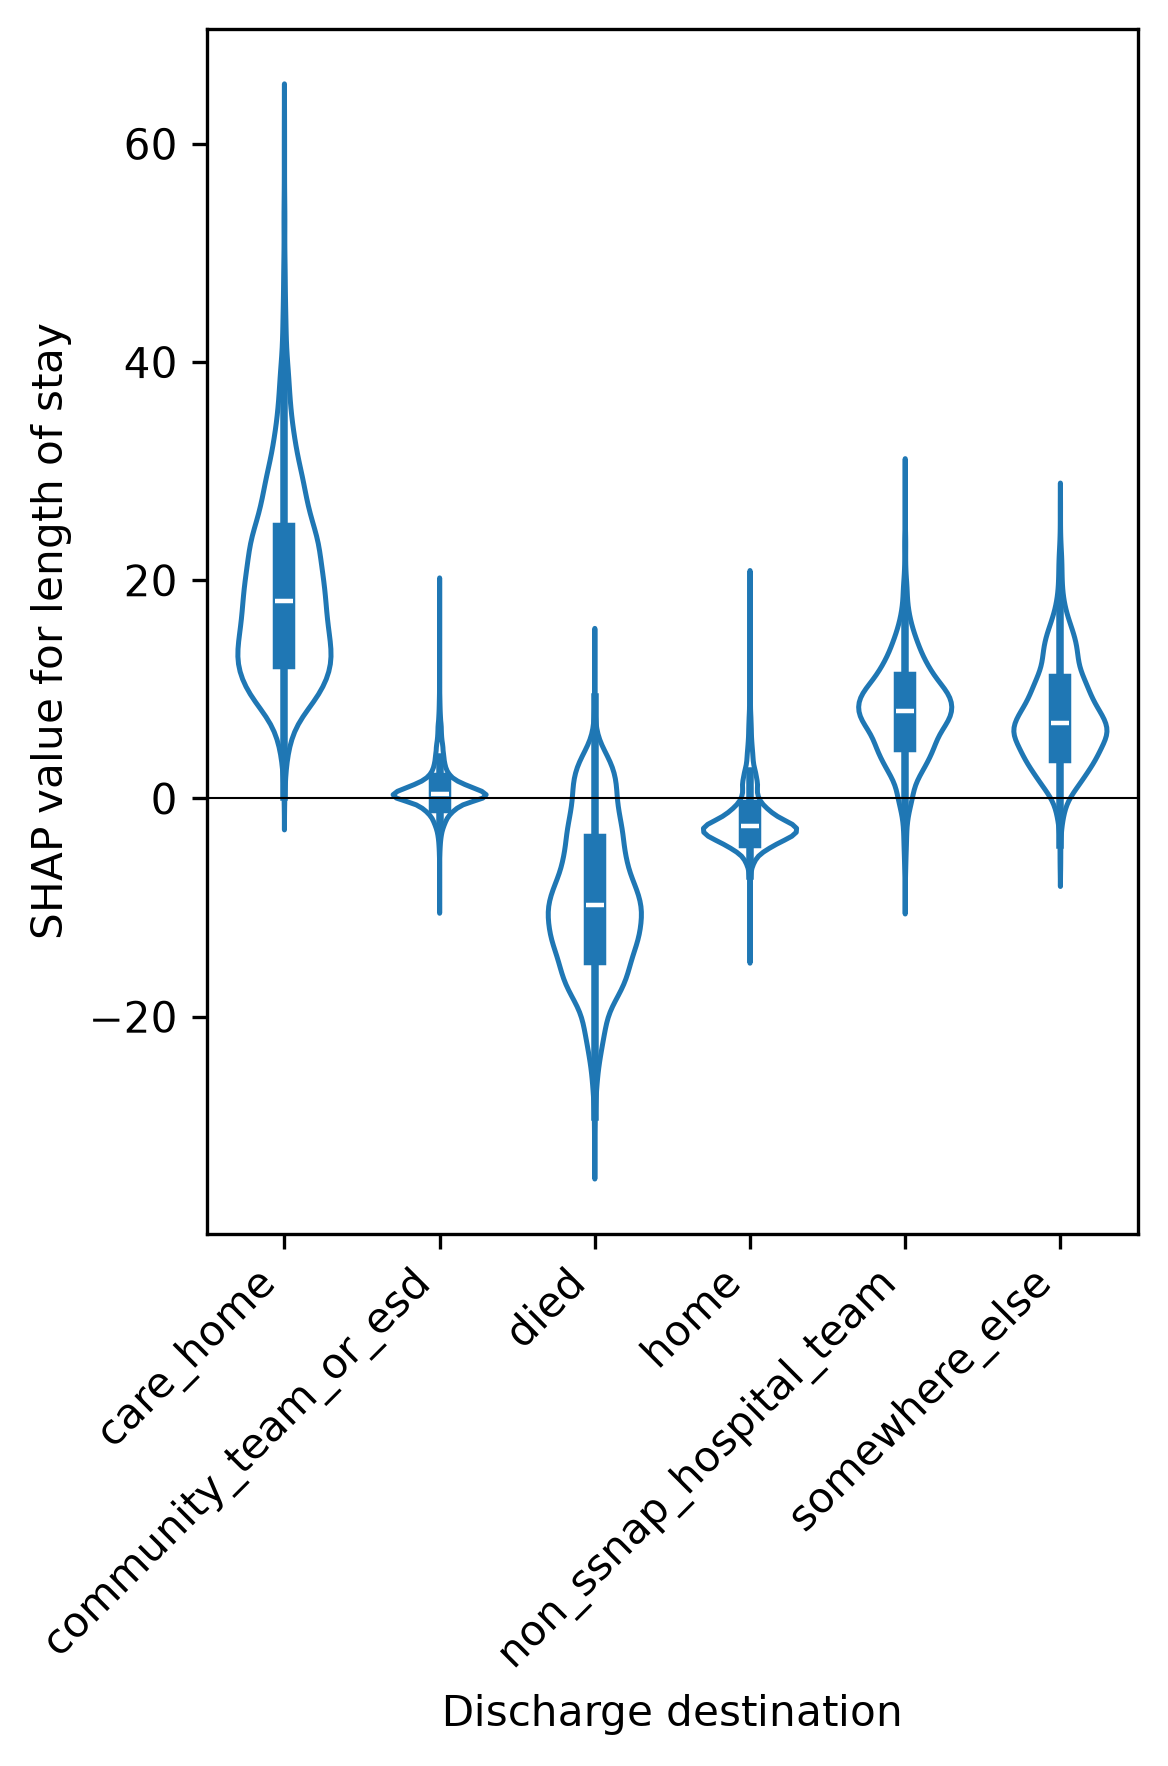
\includegraphics[width=\linewidth]{images/shap/shap_all_patients_los_discharge_destination.png}
        %\caption{}
        \label{fig:bottom-middke}
    \end{subfigure}
    \hfill
    % Bottom right image (~55% width)
    \begin{subfigure}{0.49\textwidth}
        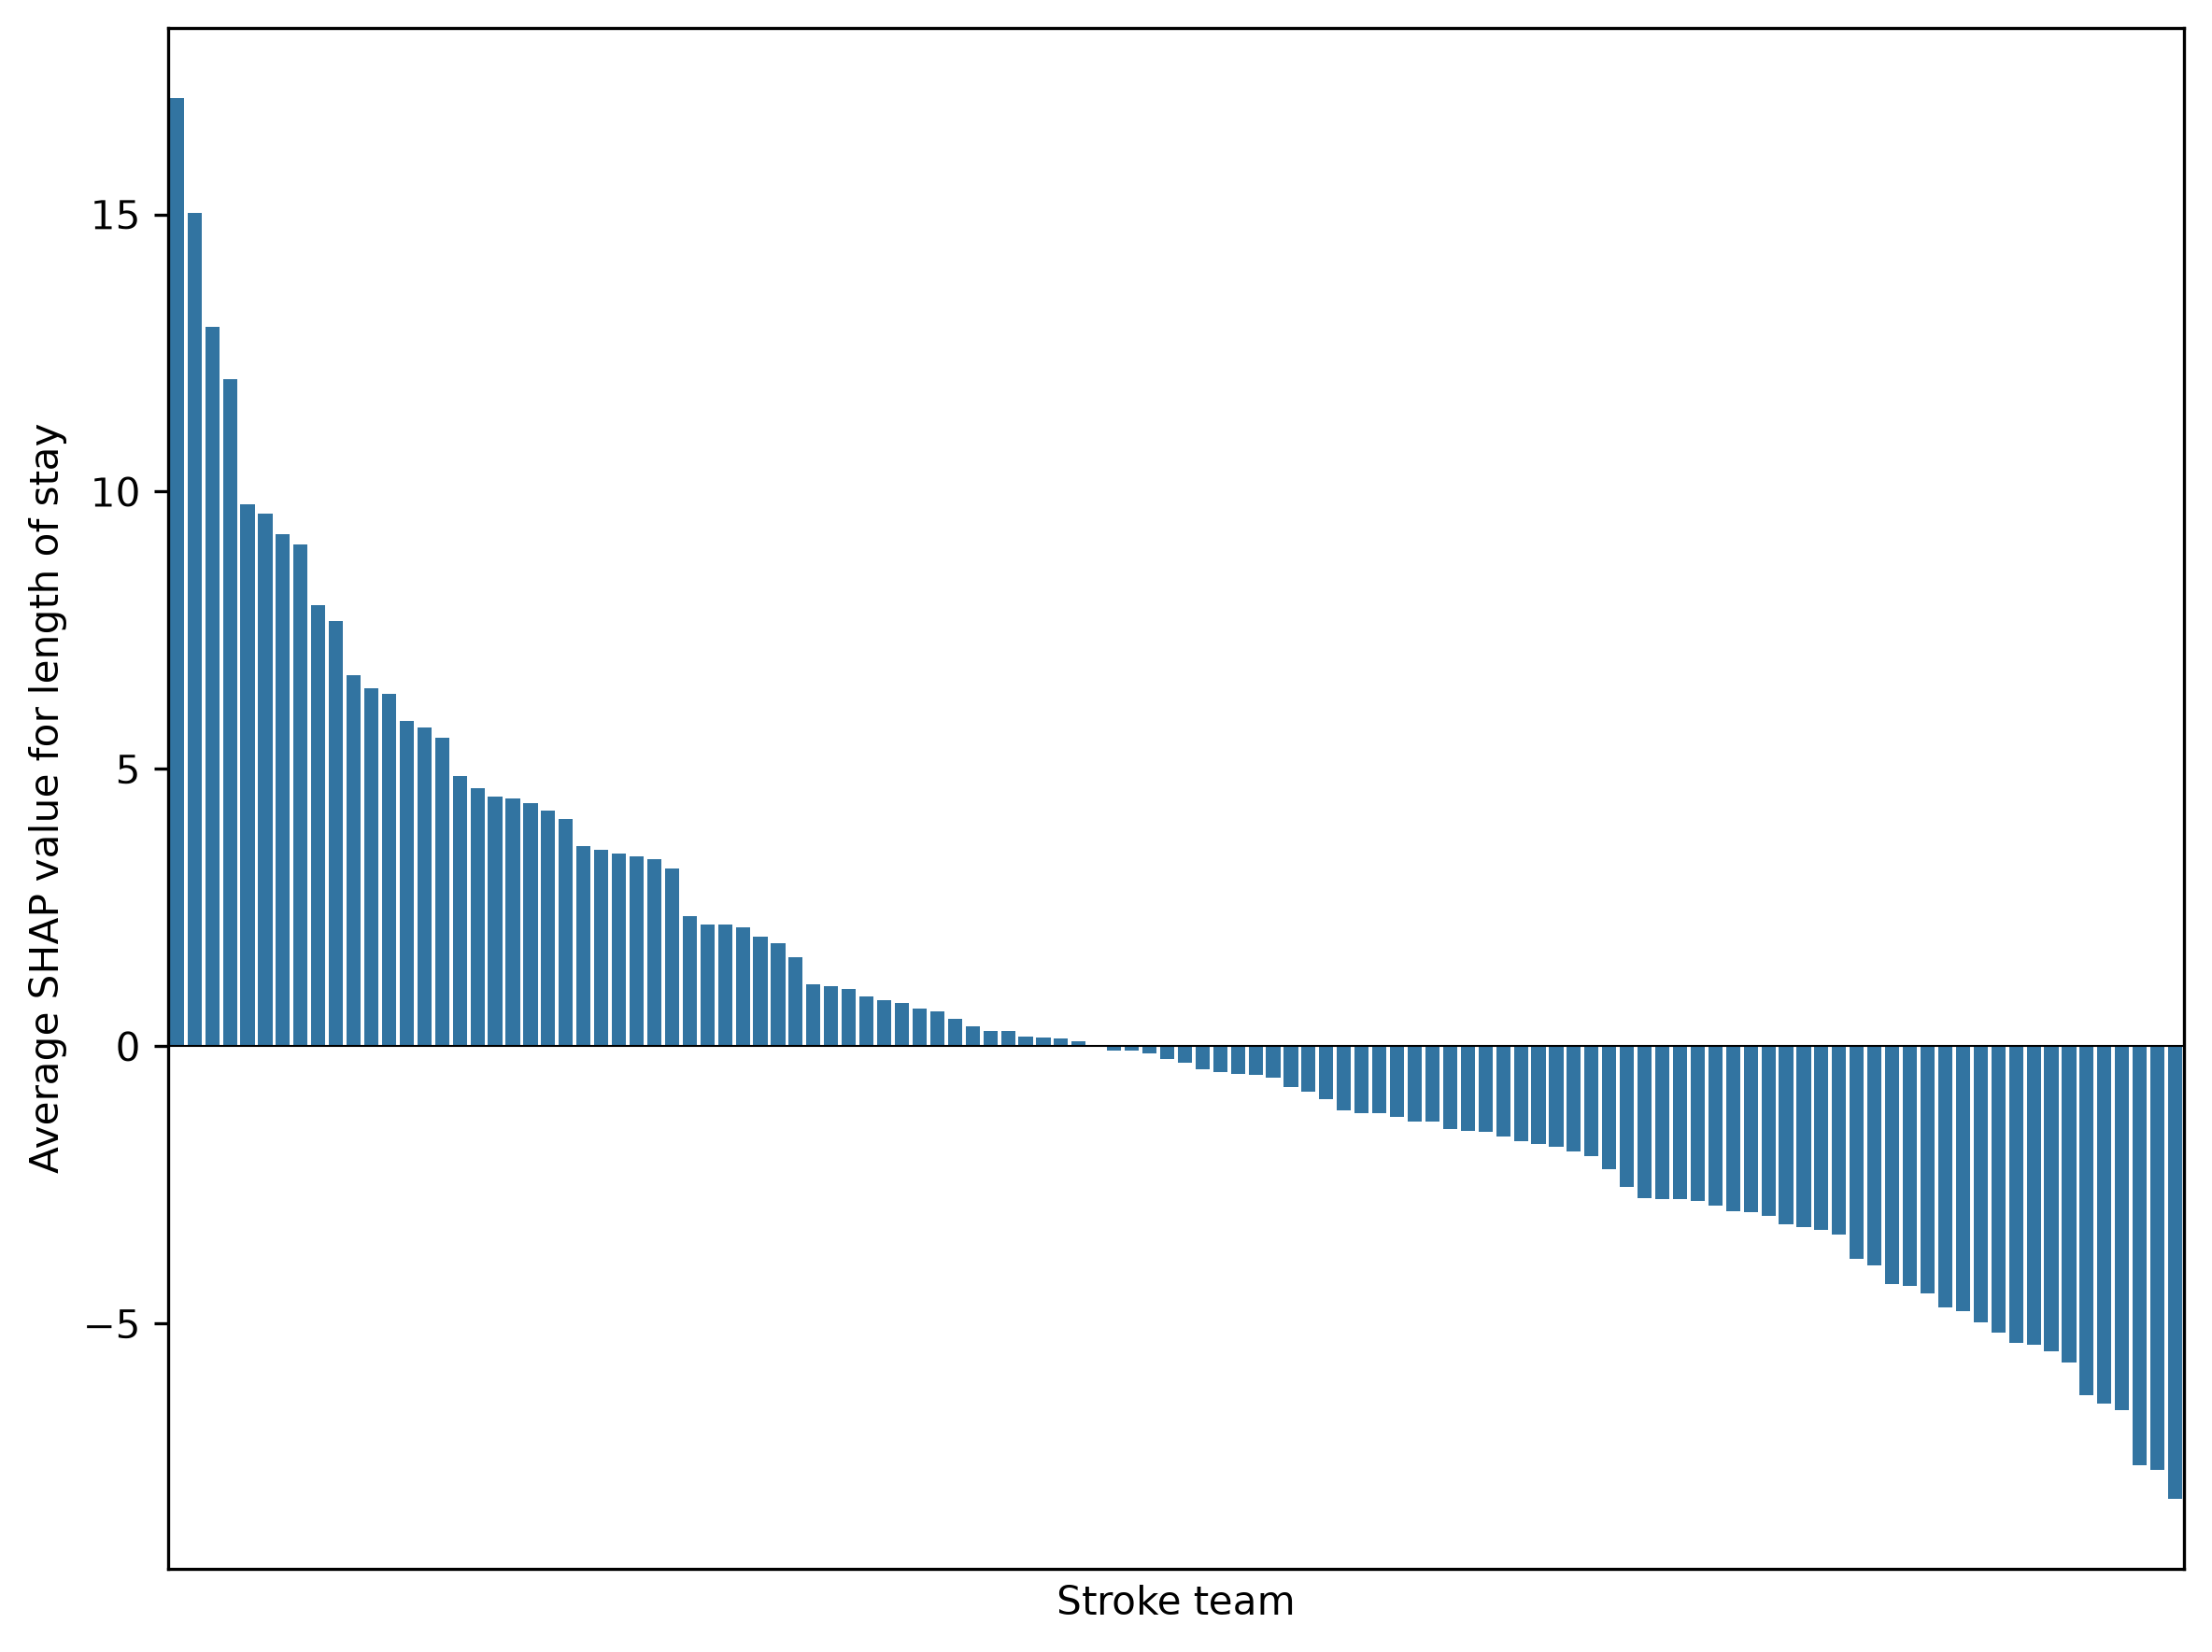
\includegraphics[width=\linewidth]{images/shap/shap_all_patients_los_stroke_team.png}
        %\caption{}
        \label{fig:bottom-right}
    \end{subfigure}

    \caption{SHAP analysis of feature contributions to predicting length of stay for stroke patients. \textit{Top}: A SHAP summary plot detailing feature impacts on the model's predictions. Each point represents an individual patient. The x-axis indicates the SHAP value, where positive values increase the predicted length of stay, and negative values decrease it. For continuous and binary variables, colour represents the original feature value (red for high; blue for low). Categorical variables (\textit{stroke team} and \textit{ethnicity}) are plotted in grey. \textit{Bottom left and middle}: Violin plots illustrating the distribution of SHAP values across ethnic groups and by discharge destination, highlighting the marginal impact of ethnicity oand discharge destination on the predicted length of stay. \textit{Bottom right}: A ranked bar chart displaying the average SHAP value for each stroke team. This visualizes institutional variation, reflecting the treating stroke team's contribution to the length of stay after accounting for patient-level clinical characteristics.}
    \label{fig:shap_los_all}
\end{figure}

%%%%%%%%%%%%%%%%%%%% Use of thrombolysis %%%%%%%%%%%%%%%%%%%%%%%%

\begin{figure}[htbp]
    \centering
    
    % Top image (Full width)
    \begin{subfigure}{0.50\textwidth}
        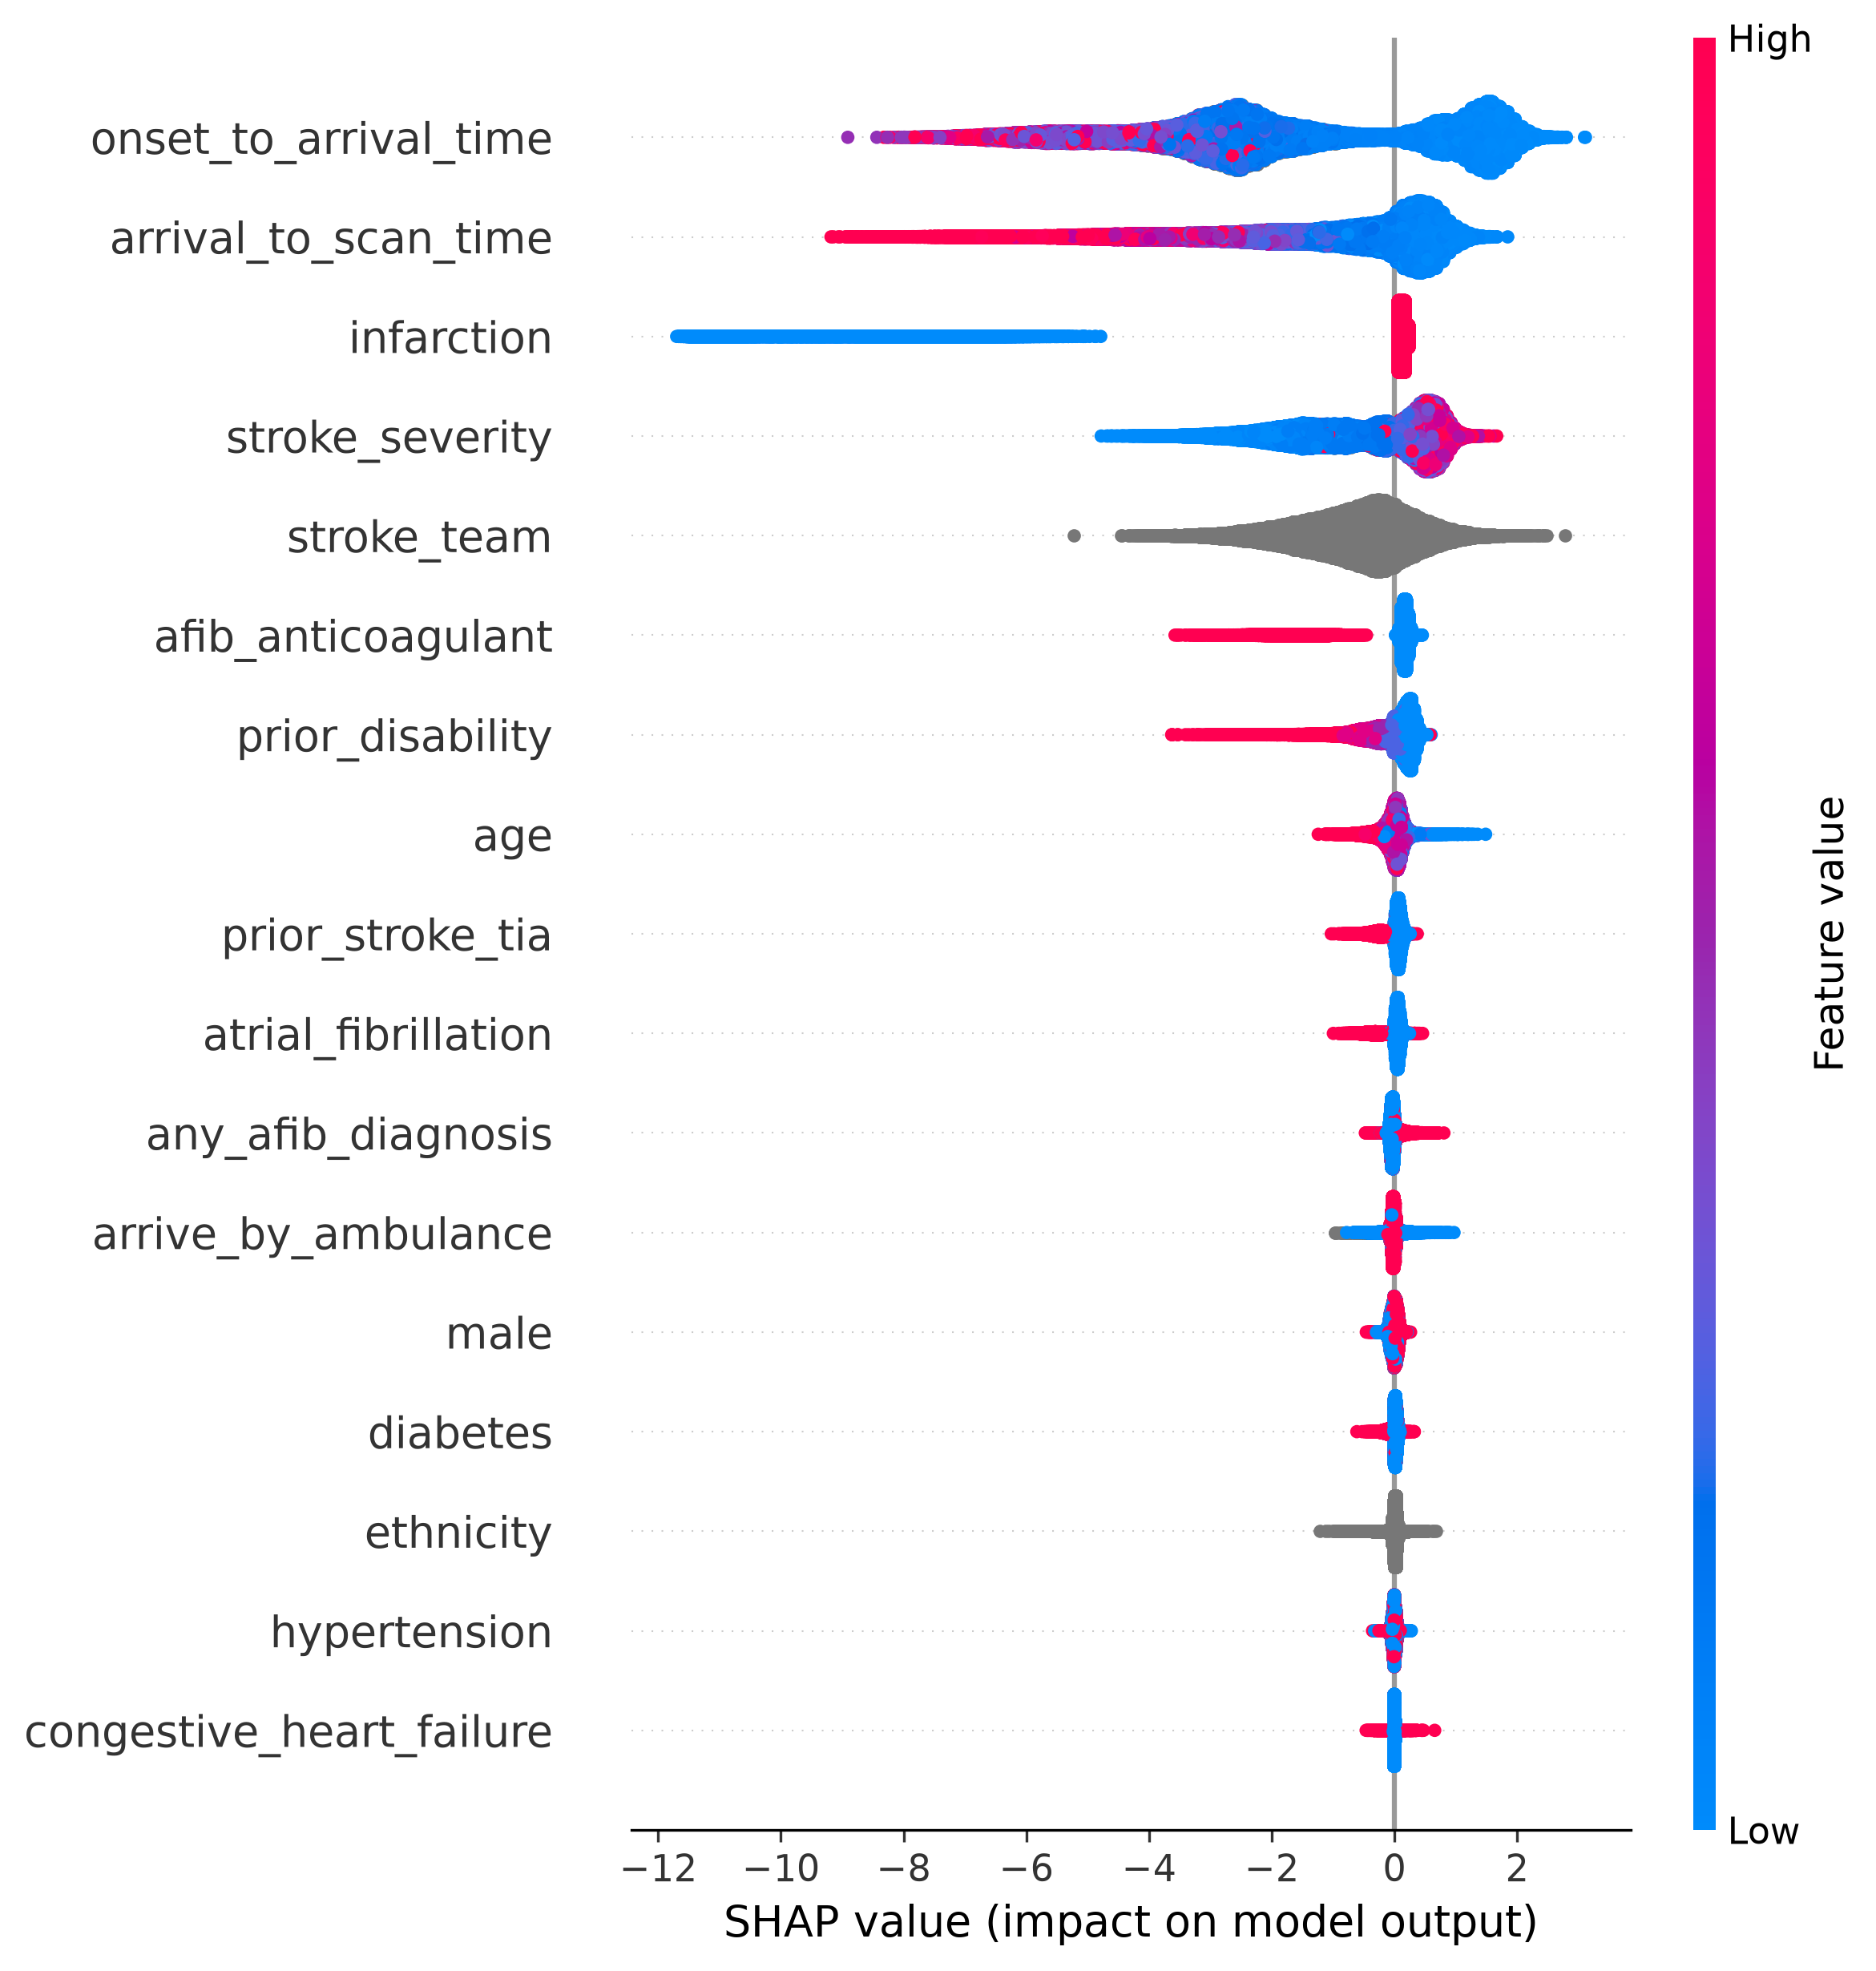
\includegraphics[width=\linewidth]{images/shap/shap_all_patients_thrombolysis_use.png}
        %\caption{}
        \label{fig:top}
    \end{subfigure}

    \vspace{0.5cm} % Optional vertical space between rows

    % Bottom left image (~45% width)
    \begin{subfigure}{0.407\textwidth}
        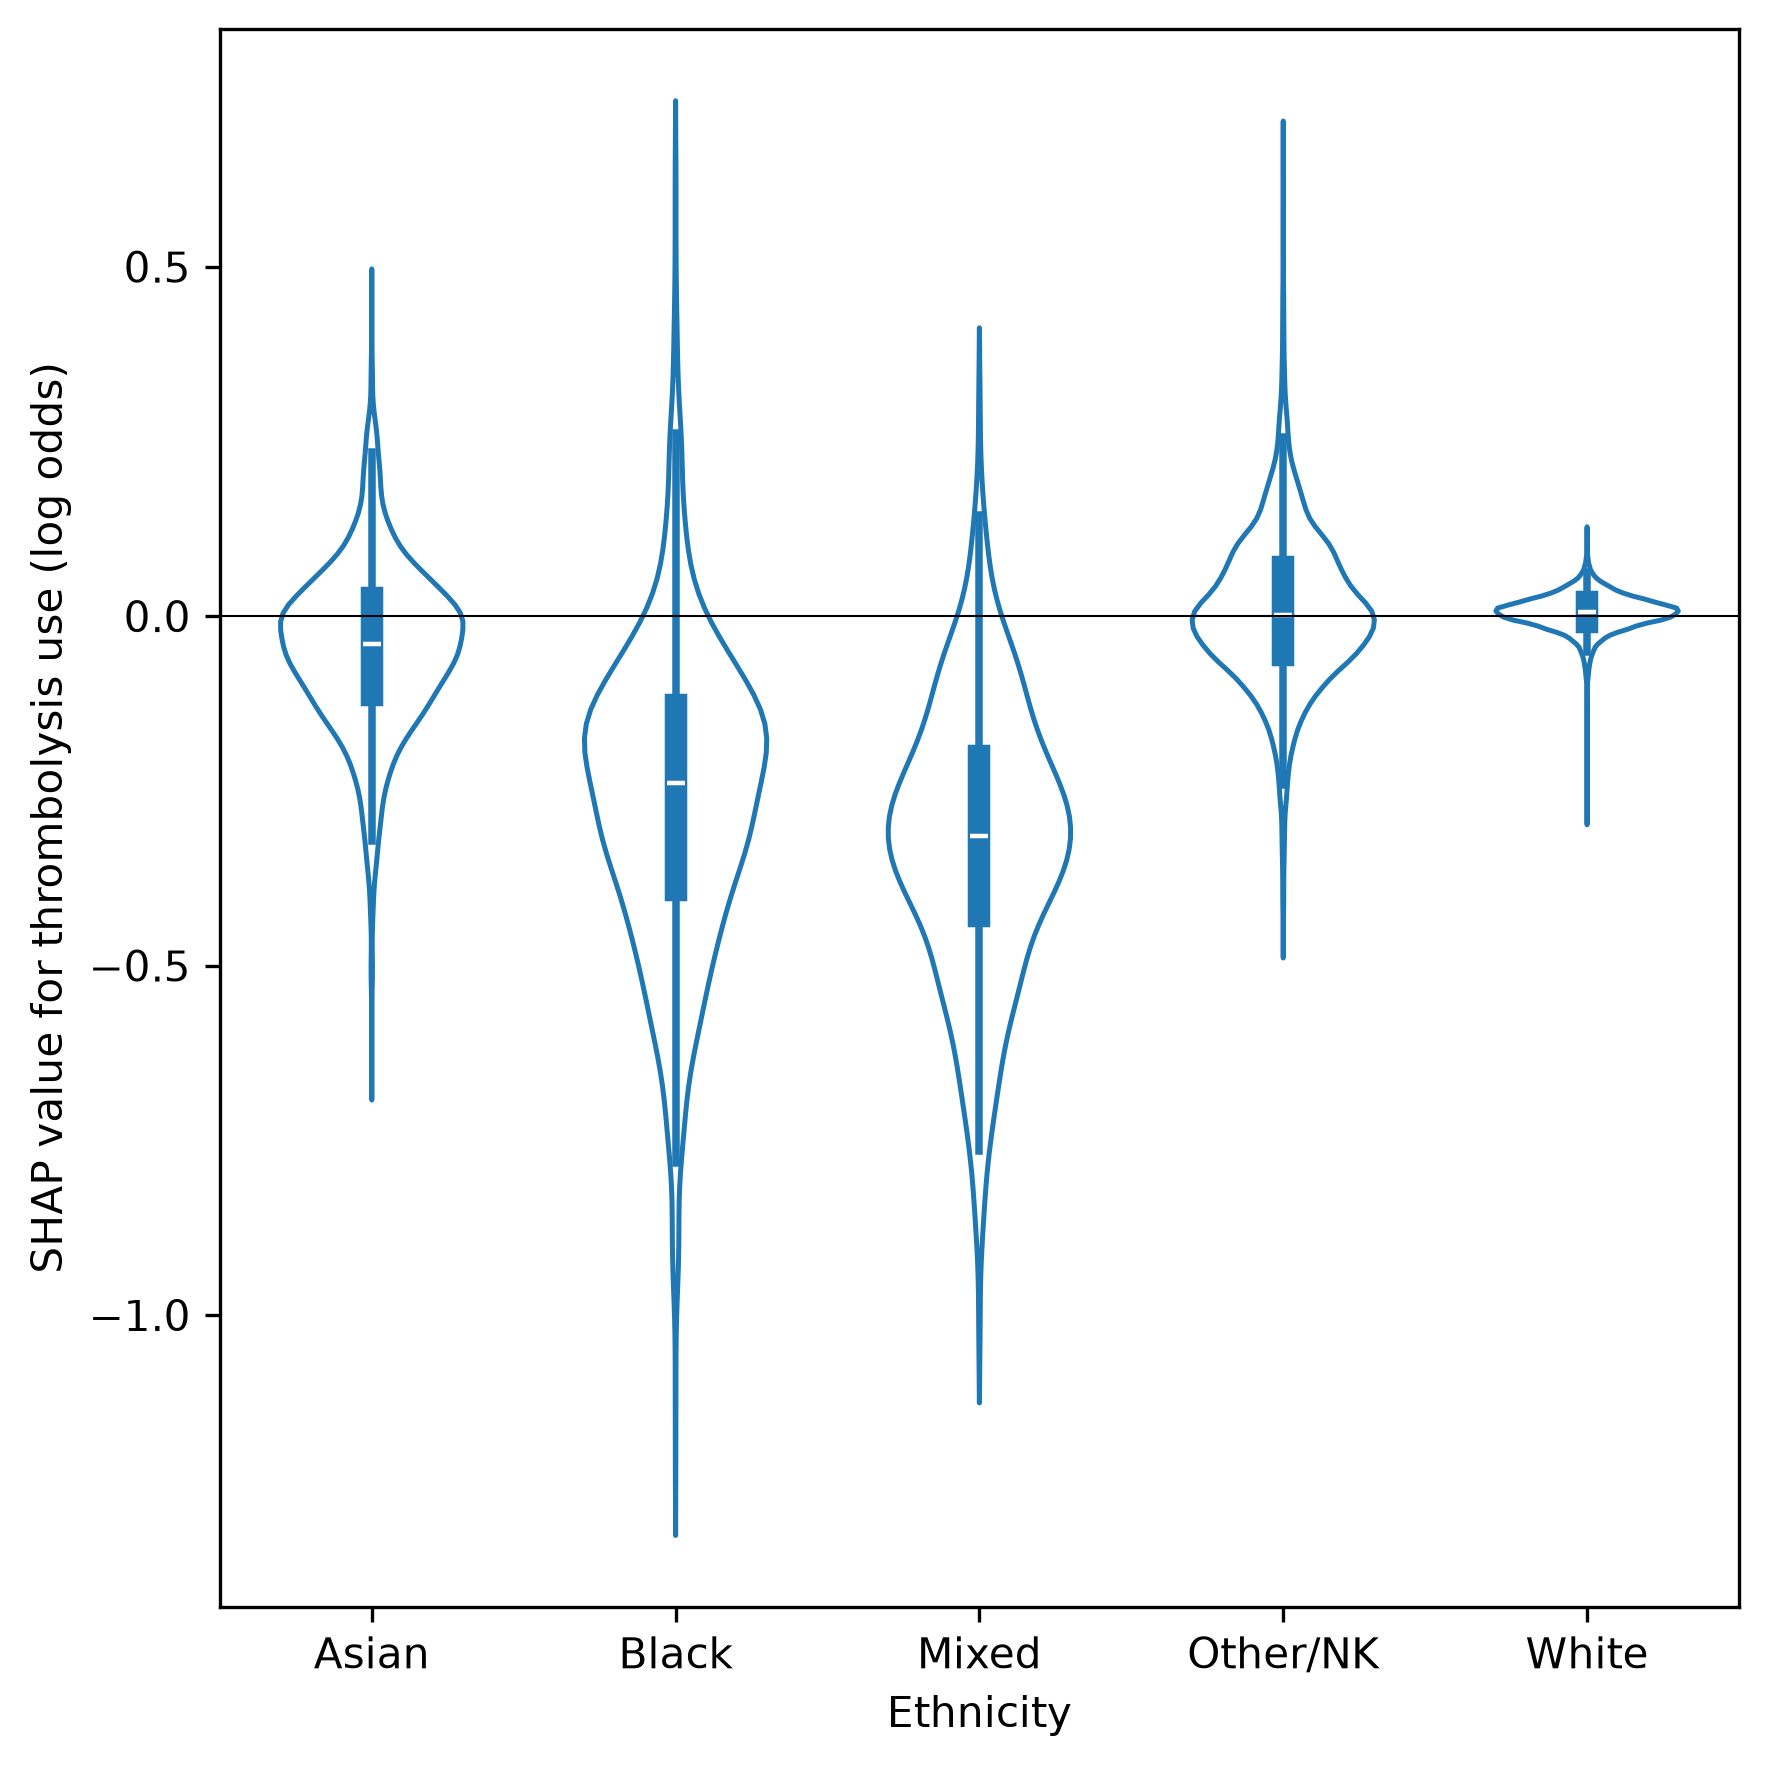
\includegraphics[width=\linewidth]{images/shap/shap_all_patients_thrombolysis_use_ethnicity.png}
        %\caption{}
        \label{fig:bottom-left}
    \end{subfigure}
    \hfill % Adds flexible horizontal spacing
    % Bottom right image (~55% width)
    \begin{subfigure}{0.543\textwidth}
        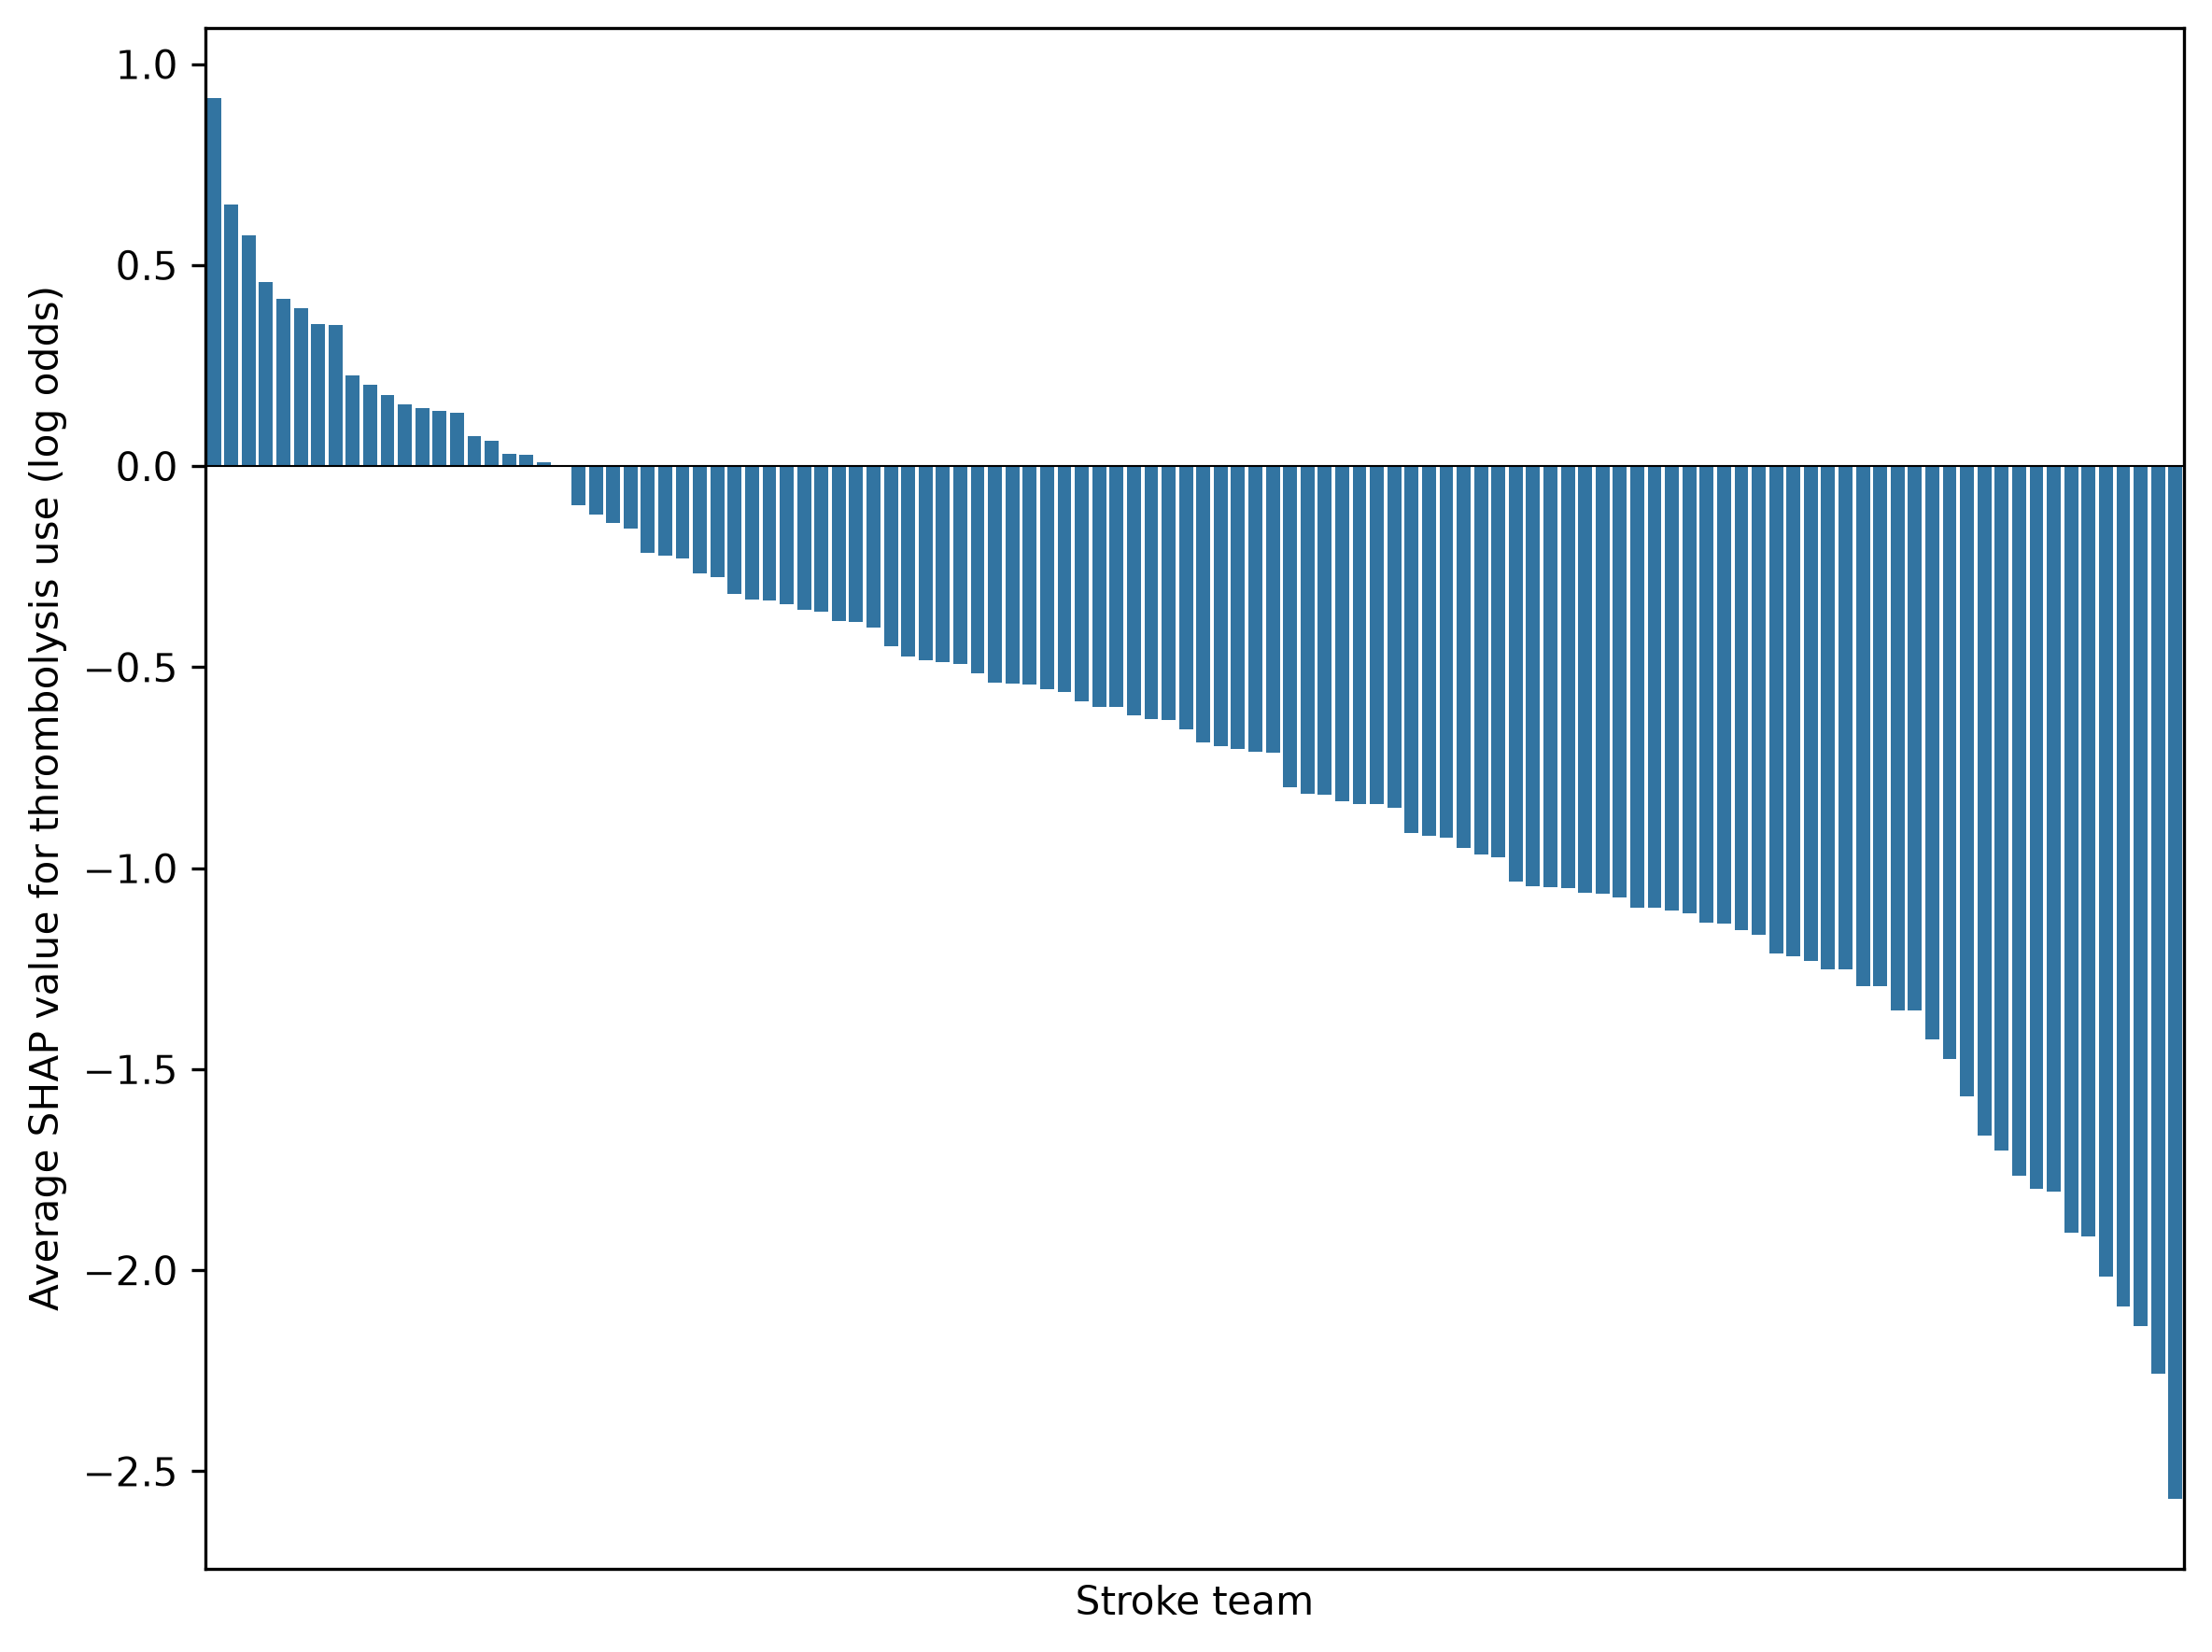
\includegraphics[width=\linewidth]{images/shap/shap_all_patients_thrombolysis_use_stroke_team.png}
        %\caption{}
        \label{fig:bottom-right}
    \end{subfigure}

    \caption{SHAP analysis of feature contributions to predicting use of thrombolysis in stroke patients. \textit{Top}: A SHAP summary plot detailing the impact of features on the model's log-odds predictions. Each point represents an individual patient instance. The position on the x-axis indicates the SHAP value, where positive values increase the predicted odds of receiving thrombolysis, and negative values decrease it. For continuous and binary variables, colour represents the original feature value (red indicating high values; blue indicating low values). Categorical variables (\textit{stroke team} and \textit{ethnicity}) are plotted in grey. \textit{Bottom left}: Violin plots illustrating the distribution of SHAP values across distinct ethnic groups. This panel highlights the marginal impact and variance of ethnicity on the model's prediction for thrombolysis use. \textit{Bottom Right}: A ranked bar chart displaying the average SHAP value associated with each individual stroke team. This panel visualizes institutional variation, reflecting the contribution of the treating stroke team to the predicted likelihood of receiving thrombolysis after accounting for patient-level clinical characteristics.}  
    \label{fig:shap_thrombolysis_all}
\end{figure}


%%%%%%%%%%%%%%%%%%%% Use of thrombectomy %%%%%%%%%%%%%%%%%%%%%%%%

\begin{figure}[htbp]
    \centering
    
    % Top image (Full width)
    \begin{subfigure}{0.50\textwidth}
        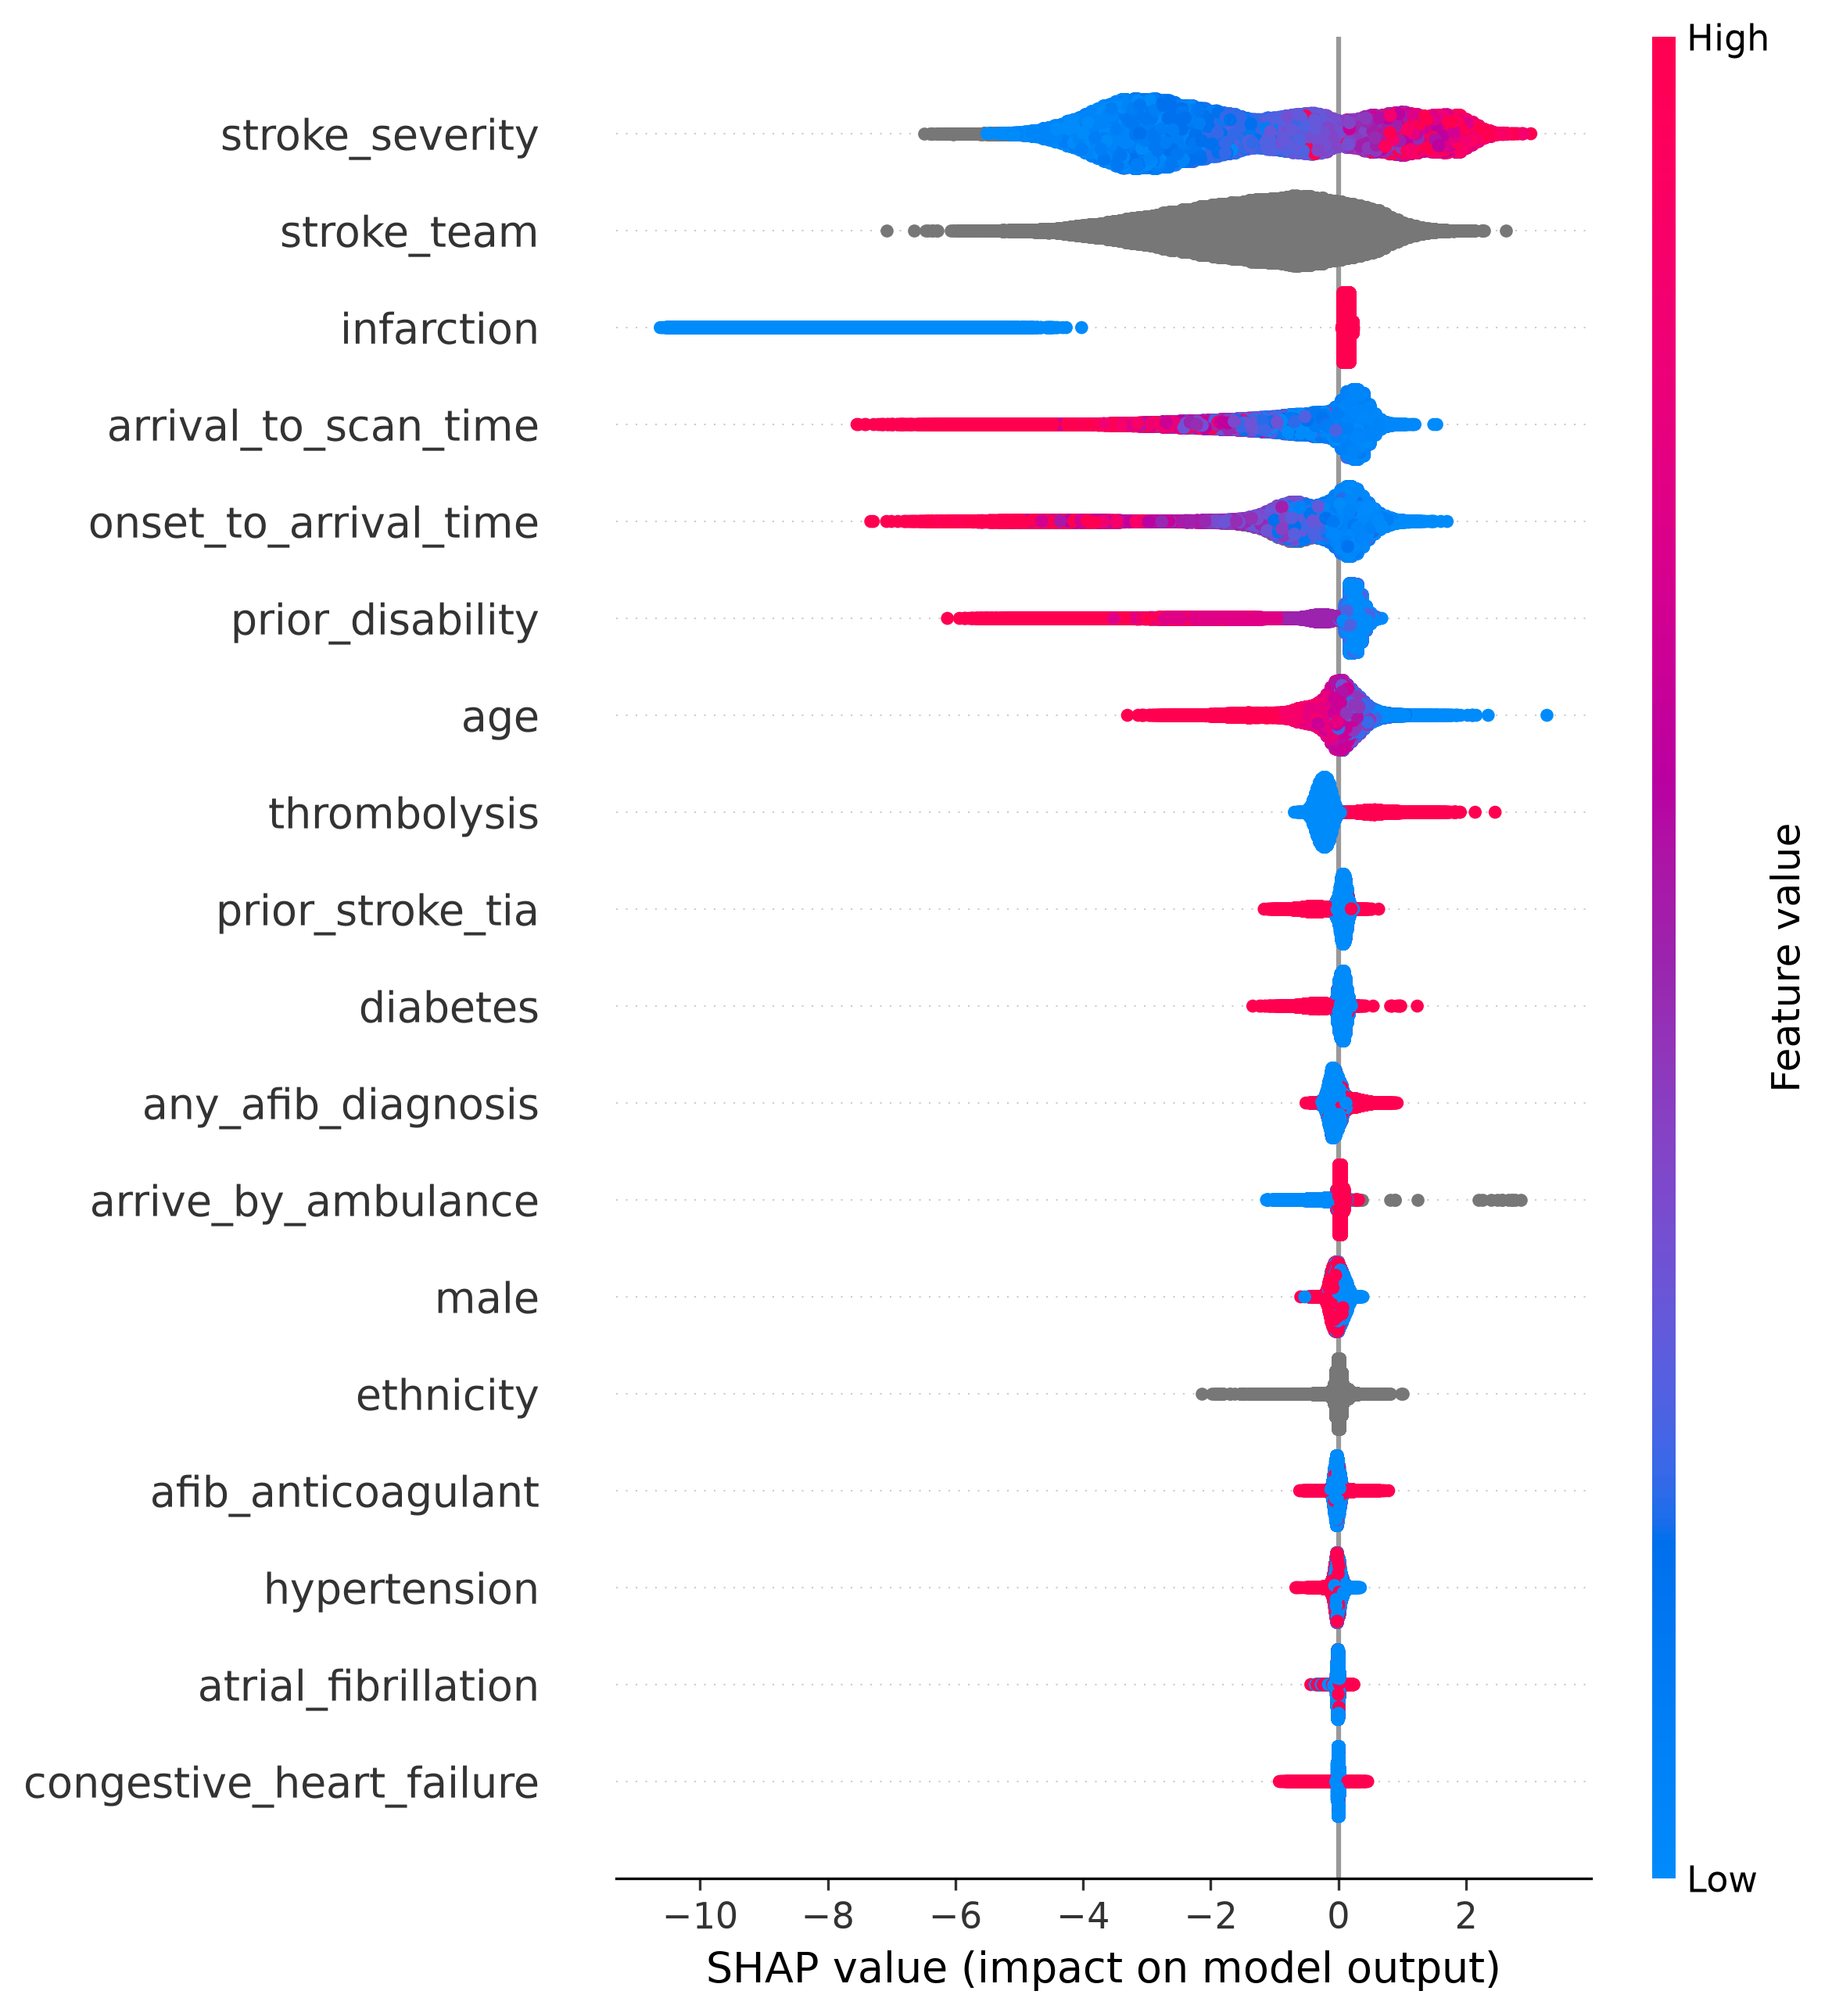
\includegraphics[width=\linewidth]{images/shap/shap_all_patients_thrombectomy_use.png}
        %\caption{}
        \label{fig:top}
    \end{subfigure}

    \vspace{0.5cm} % Optional vertical space between rows

    % Bottom left image (~45% width)
    \begin{subfigure}{0.407\textwidth}
        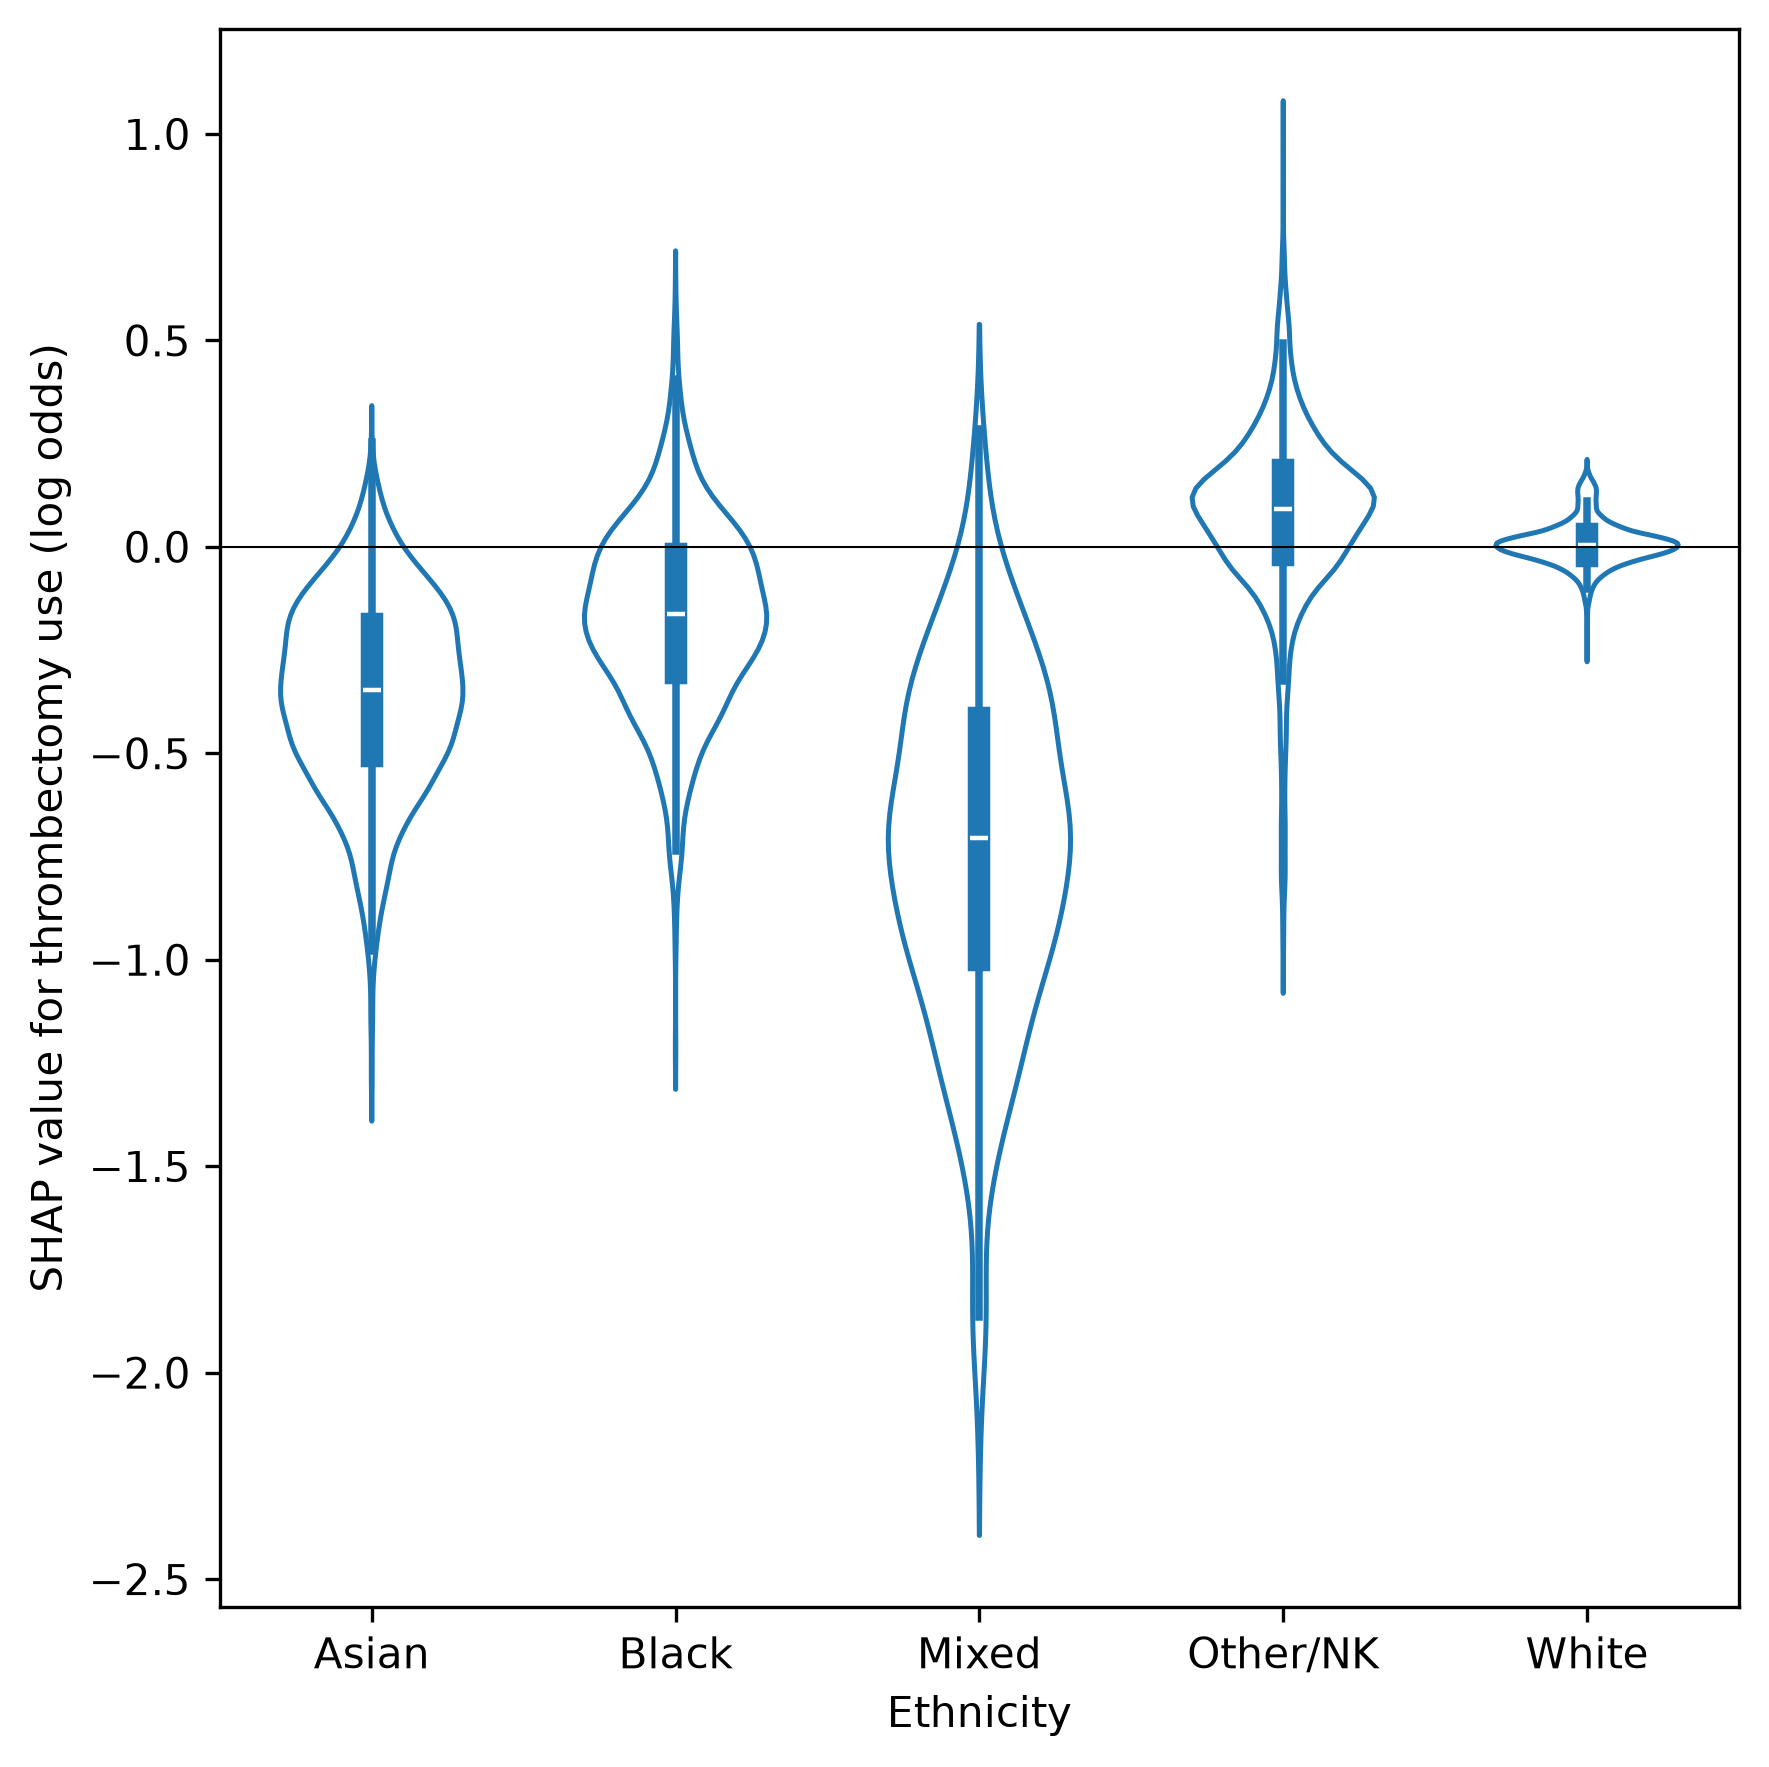
\includegraphics[width=\linewidth]{images/shap/shap_all_patients_thrombectomy_use_ethnicity.png}
        %\caption{}
        \label{fig:bottom-left}
    \end{subfigure}
    \hfill % Adds flexible horizontal spacing
    % Bottom right image (~55% width)
    \begin{subfigure}{0.543\textwidth}
        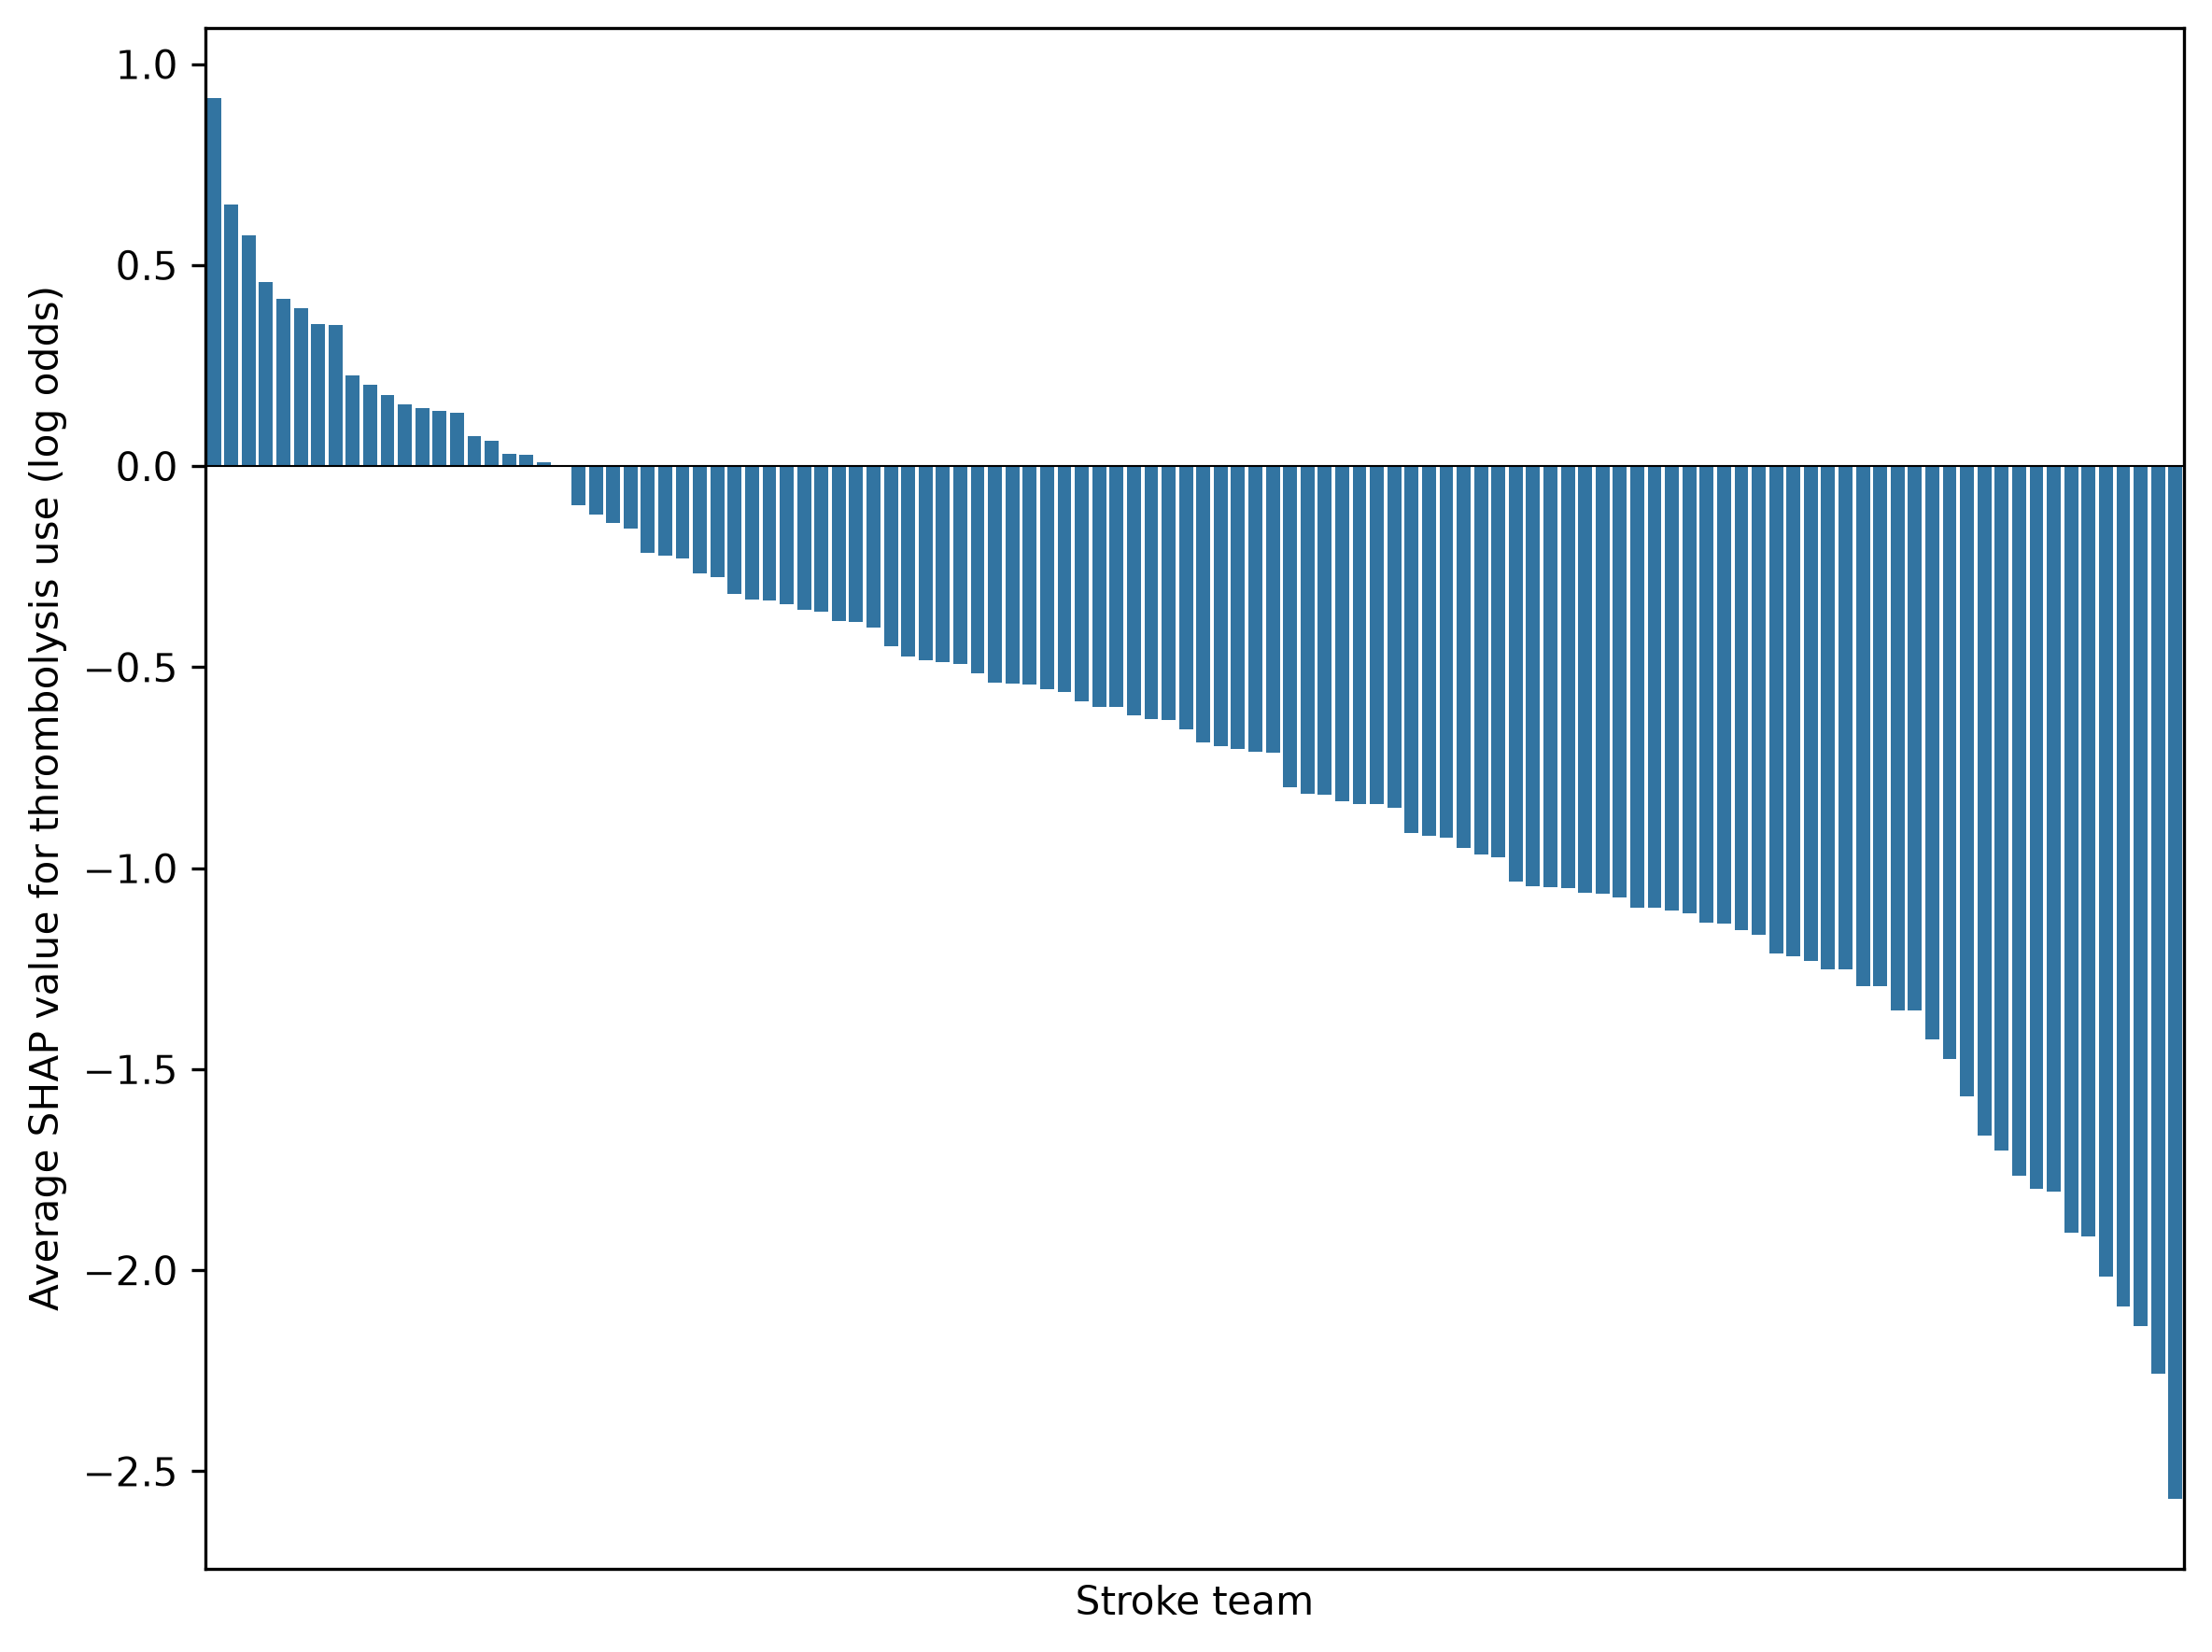
\includegraphics[width=\linewidth]{images/shap/shap_all_patients_thrombolysis_use_stroke_team.png}
        %\caption{}
        \label{fig:bottom-right}
    \end{subfigure}

    \caption{SHAP analysis of feature contributions to predicting use of thrombectomy in stroke patients. \textit{Top}: A SHAP summary plot detailing the impact of features on the model's log-odds predictions. Each point represents an individual patient instance. The position on the x-axis indicates the SHAP value, where positive values increase the predicted odds of receiving thrombectomy, and negative values decrease it. For continuous and binary variables, colour represents the original feature value (red indicating high values; blue indicating low values). Categorical variables (\textit{stroke team} and \textit{ethnicity}) are plotted in grey. \textit{Bottom left}: Violin plots illustrating the distribution of SHAP values across distinct ethnic groups. This panel highlights the marginal impact and variance of ethnicity on the model's prediction for thrombectomy use. \textit{Bottom Right}: A ranked bar chart displaying the average SHAP value associated with each individual stroke team. This panel visualizes institutional variation, reflecting the contribution of the treating stroke team to the predicted likelihood of receiving thrombectomy after accounting for patient-level clinical characteristics.}  
    \label{fig:shap_thrombectomy_all}
\end{figure}


%%%%%%%%%%%%%%%%%%%% Thrombolysis-induced haemorrhage %%%%%%%%%%%%%%%%%%%%%%%%

\begin{figure}[htbp]
    \centering
    
    % Top image (Full width)
    \begin{subfigure}{0.50\textwidth}
        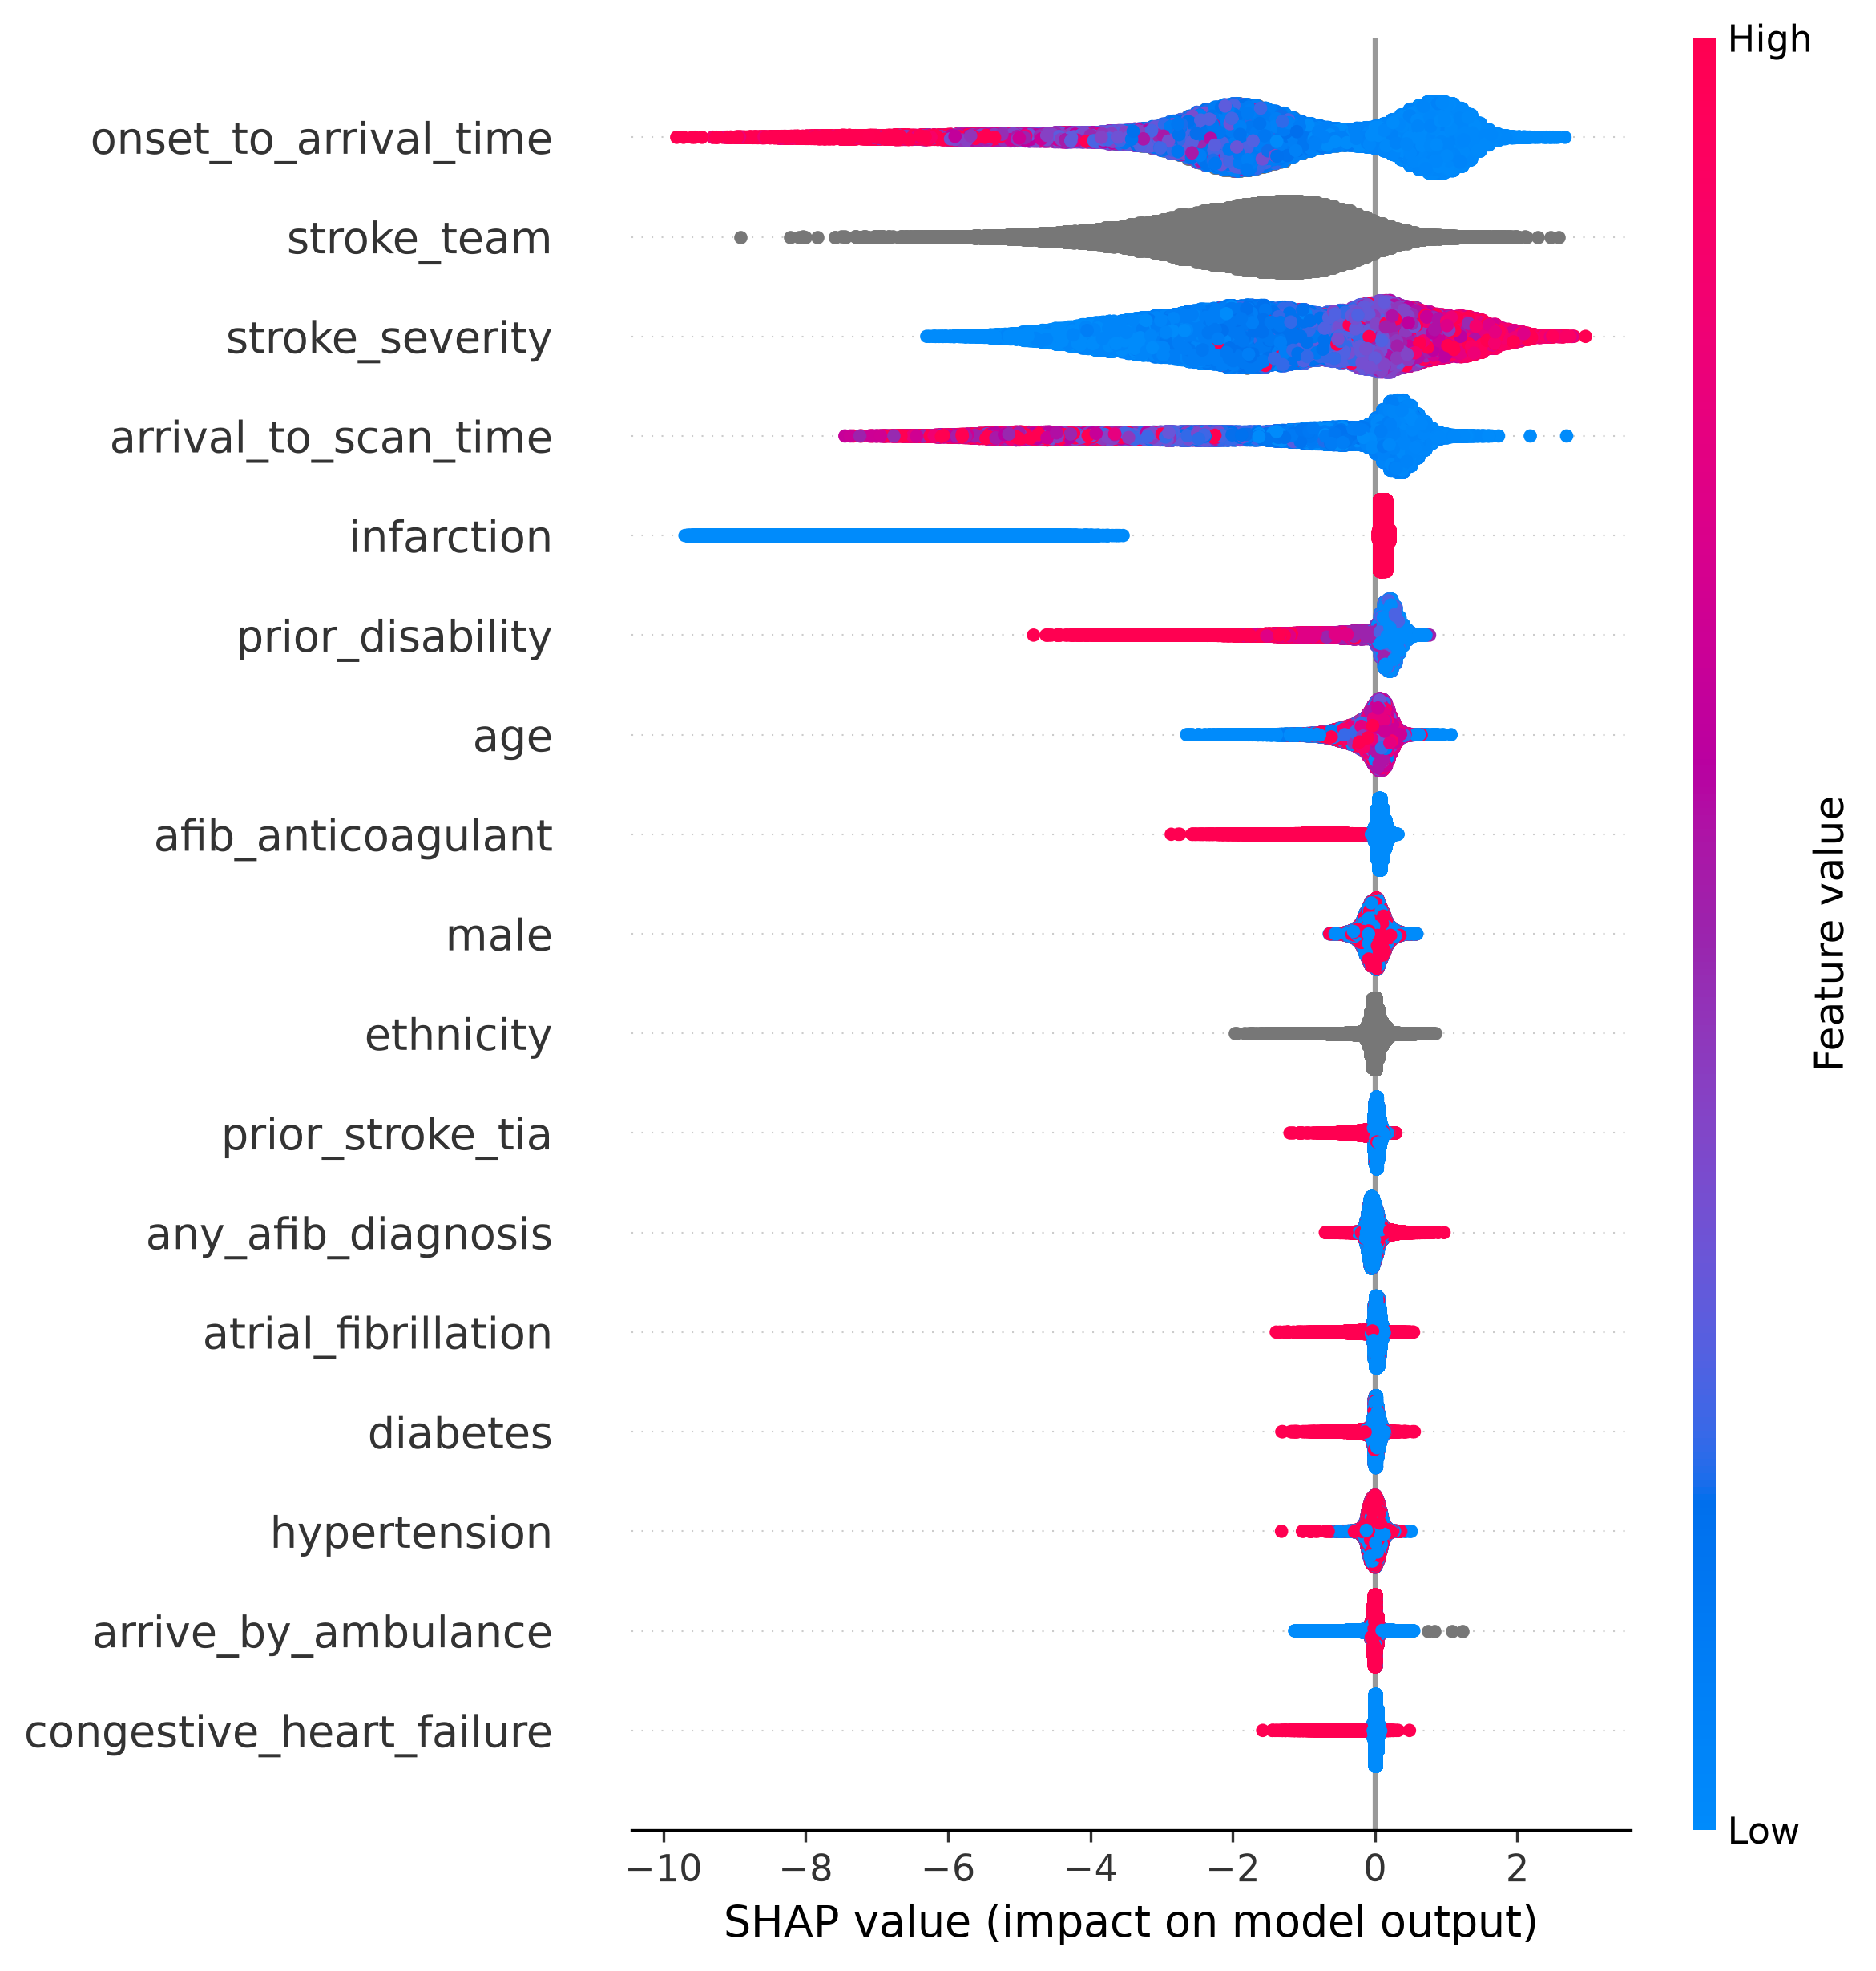
\includegraphics[width=\linewidth]{images/shap/shap_thrombolysis_induced_haemorrhage_use.png}
        %\caption{}
        \label{fig:top}
    \end{subfigure}

    \vspace{0.5cm} % Optional vertical space between rows

    % Bottom left image (~45% width)
    \begin{subfigure}{0.407\textwidth}
        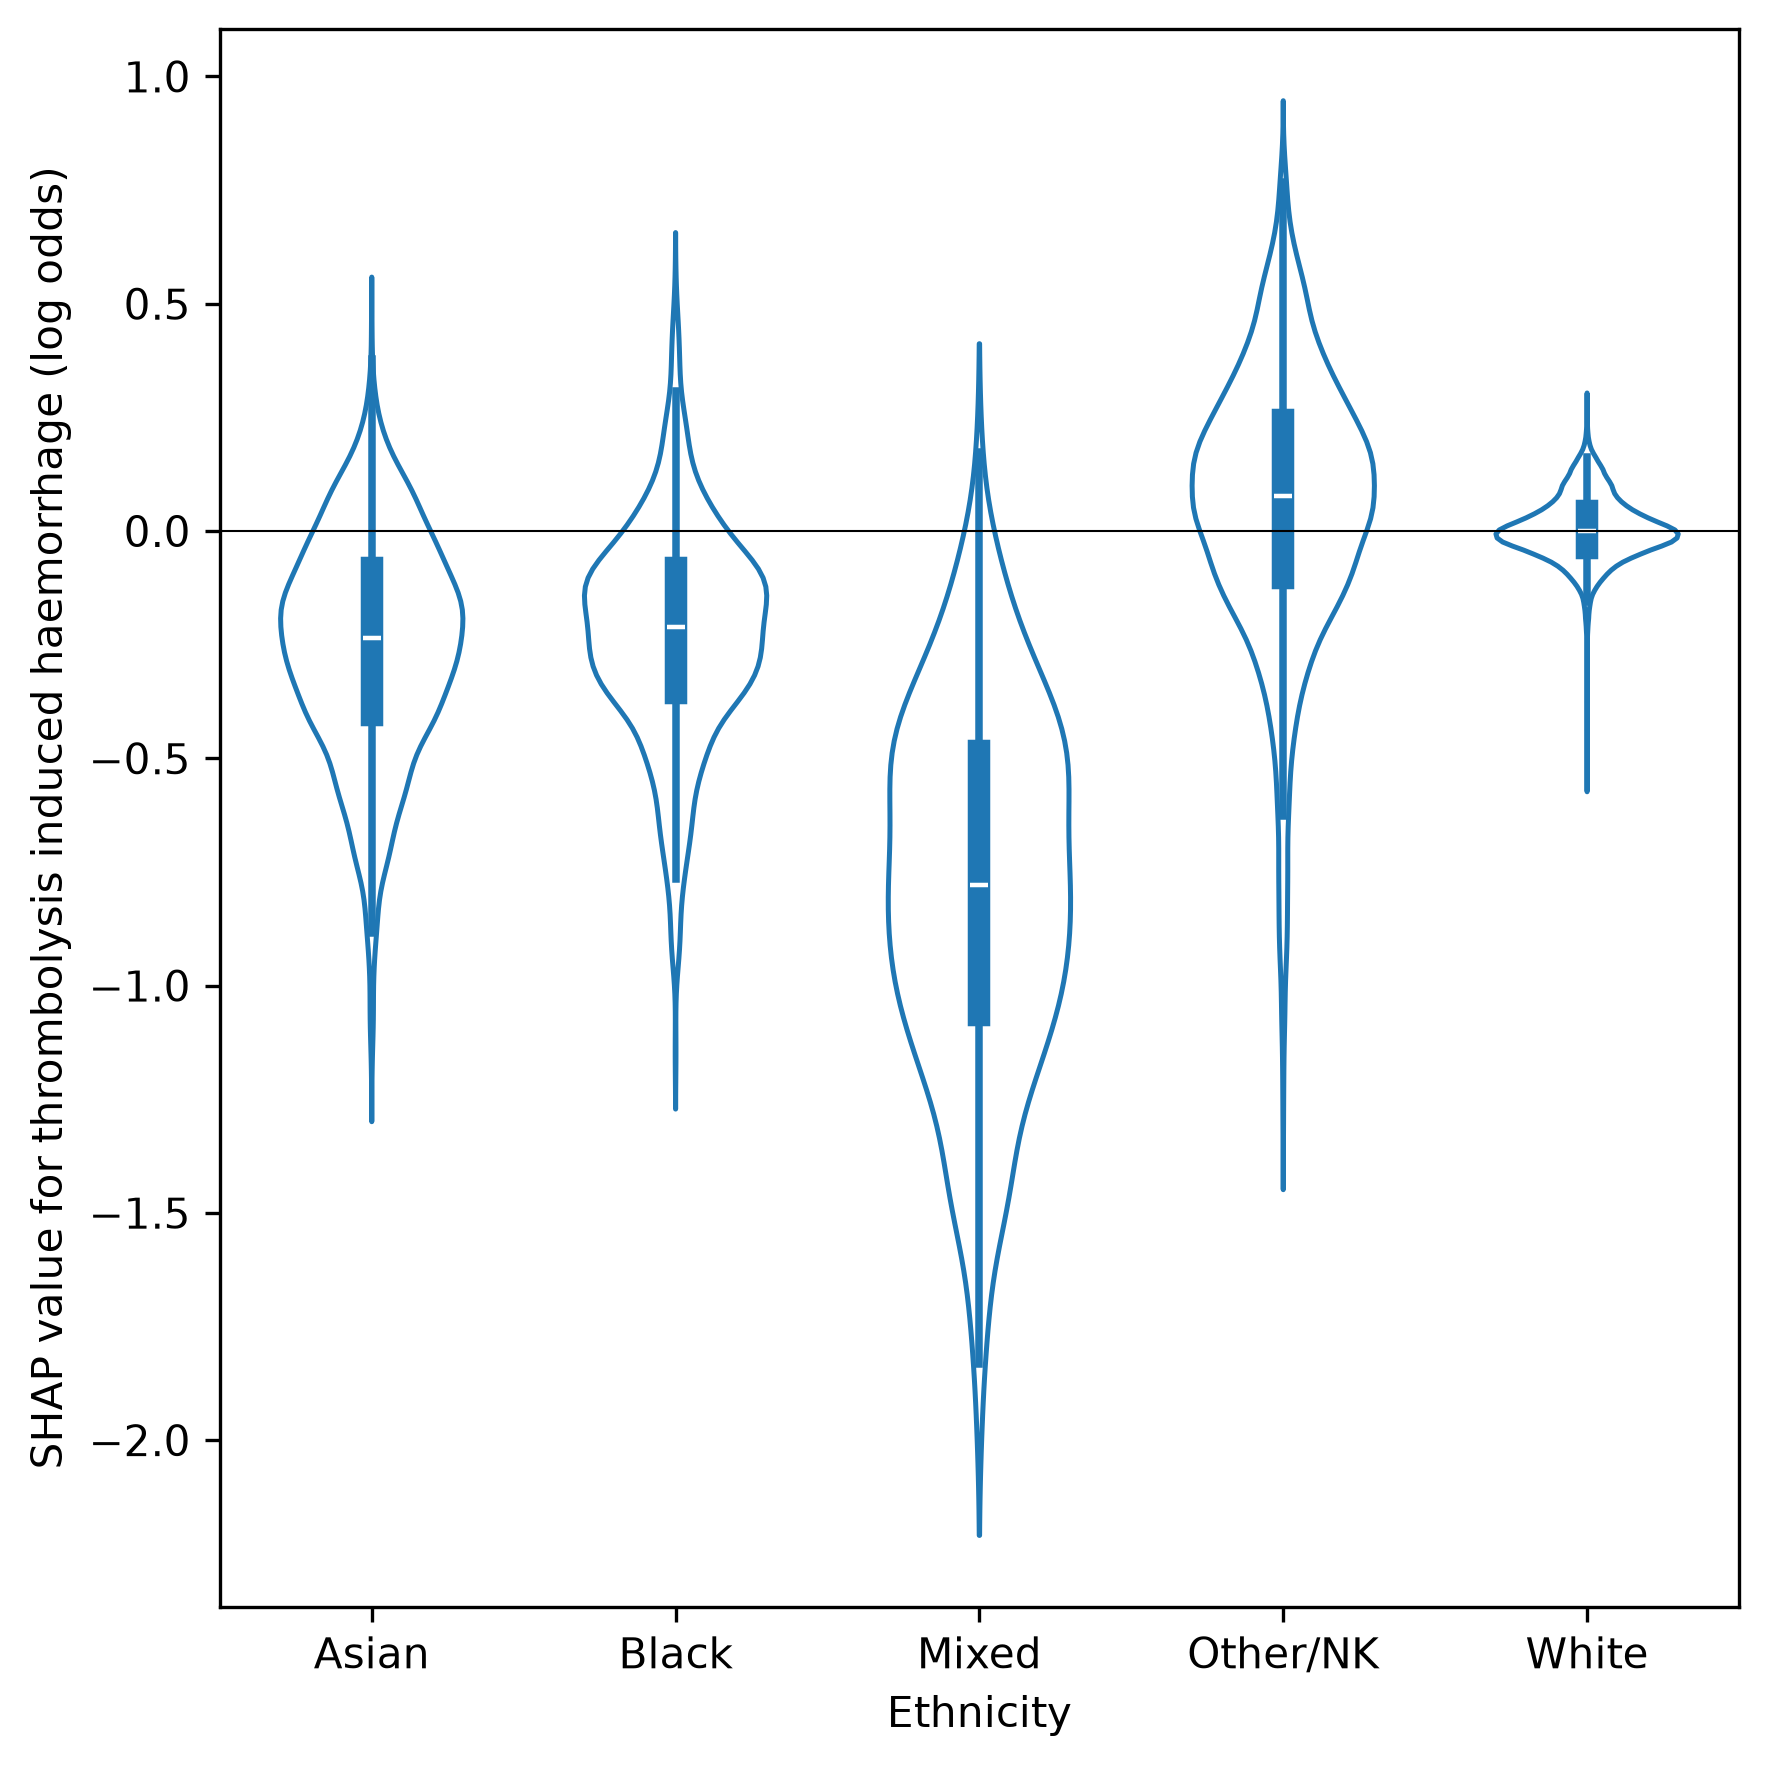
\includegraphics[width=\linewidth]{images/shap/shap_thrombolysis_induced_haemorrhage_use_ethnicity.png}
        %\caption{}
        \label{fig:bottom-left}
    \end{subfigure}
    \hfill % Adds flexible horizontal spacing
    % Bottom right image (~55% width)
    \begin{subfigure}{0.543\textwidth}
        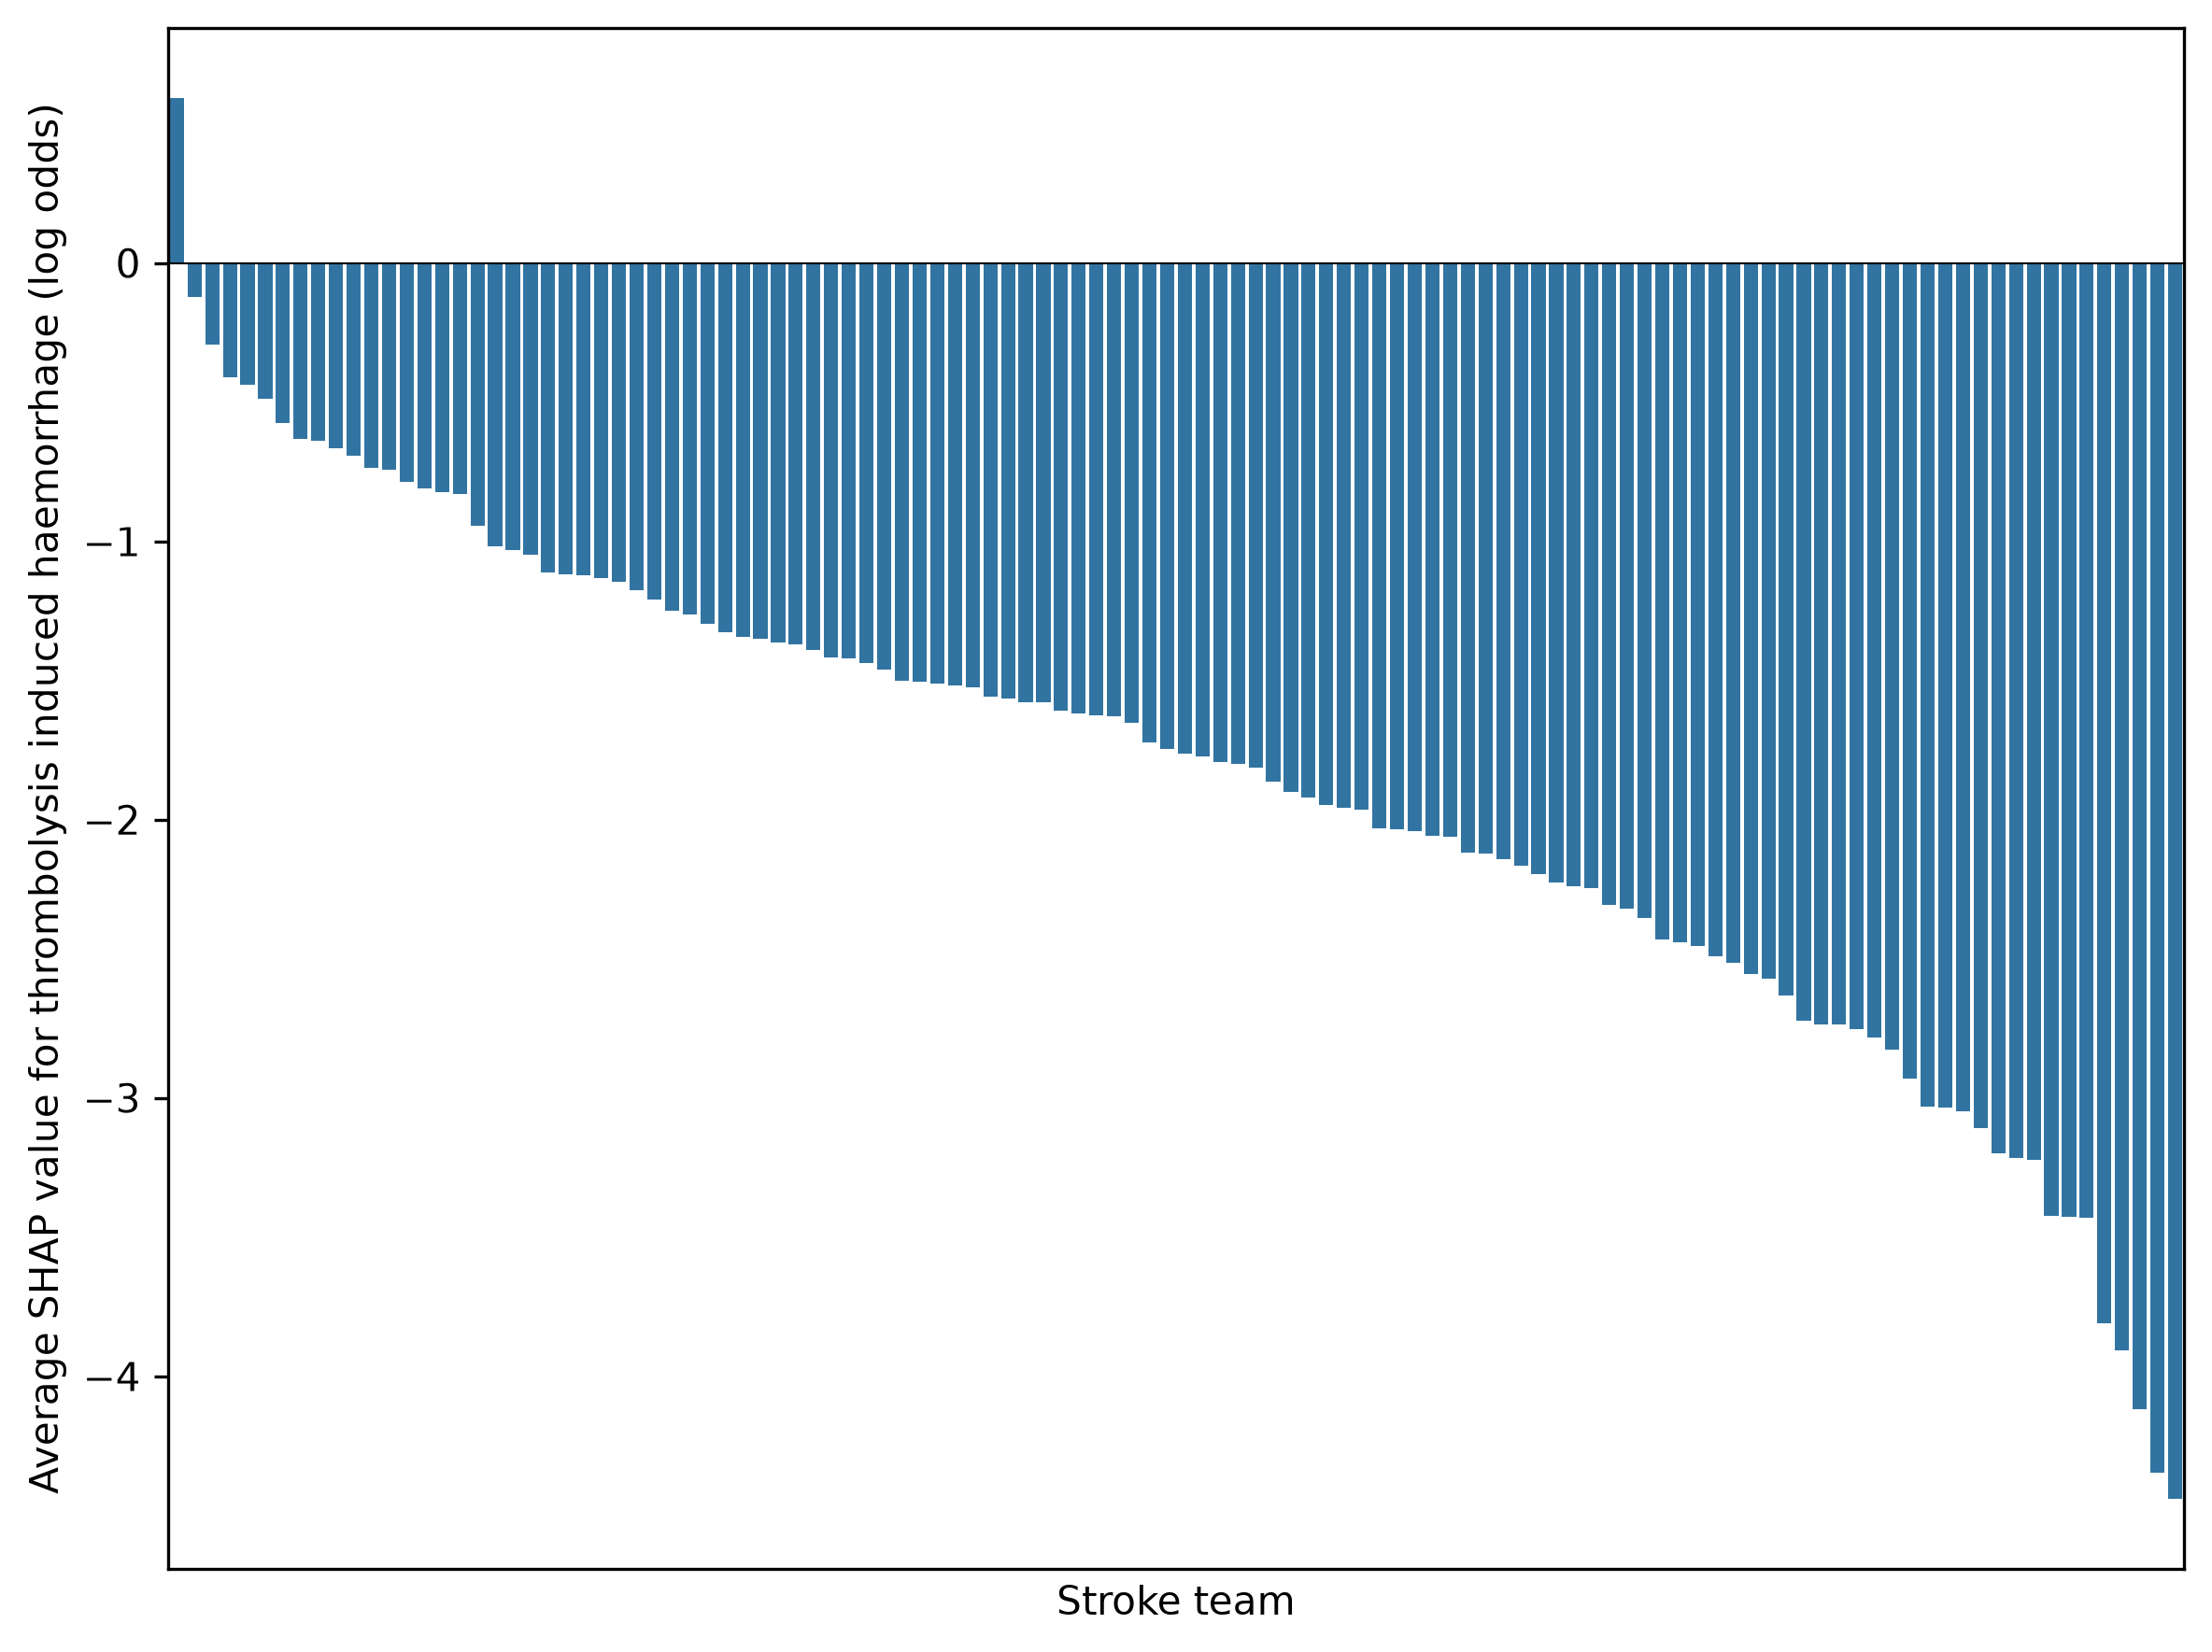
\includegraphics[width=\linewidth]{images/shap/shap_thrombolysis_induced_haemorrhage_use_stroke_team.png}
        %\caption{}
        \label{fig:bottom-right}
    \end{subfigure}
    \caption{SHAP analysis of feature contributions to predicting thrombolysis-induced haemorrhage in stroke patients who have received thrombolysis. \textit{Top}: A SHAP summary plot detailing the impact of features on the model's log-odds predictions. Each point represents an individual patient instance. The position on the x-axis indicates the SHAP value, where positive values increase the predicted odds of haemorrhage, and negative values decrease it. For continuous and binary variables, colour represents the original feature value (red indicating high values; blue indicating low values). Categorical variables (\textit{stroke team} and \textit{ethnicity}) are plotted in grey. \textit{Bottom left}: Violin plots illustrating the distribution of SHAP values across distinct ethnic groups. This panel highlights the marginal impact and variance of ethnicity on the model's prediction for haemorrhage risk. \textit{Bottom Right}: A ranked bar chart displaying the average SHAP value associated with each individual stroke team. This panel visualizes institutional variation, reflecting the contribution of the treating stroke team to the predicted risk of thrombolysis-induced haemorrhage after accounting for patient-level clinical characteristics.}
    \label{fig:shap_thrombolysis_haemorrhage}
\end{figure}


% ====================================================================================

\newpage

\section{Treatment effects}

\subsection{Target trial emulation}

Figures \ref{fig:target_trial_mrs_1} to \ref{fig:target_trial_mrs_5} show treatment effect estimates, estimated using matching-based target trial emulation, for achieving each possible mRS threshold. Treatment effects are shown as a change in average discharge mRS (this is the same in all charts) and the change in probability in being discharged at, or below, each mRS threshold.

\begin{figure}
    \centering
    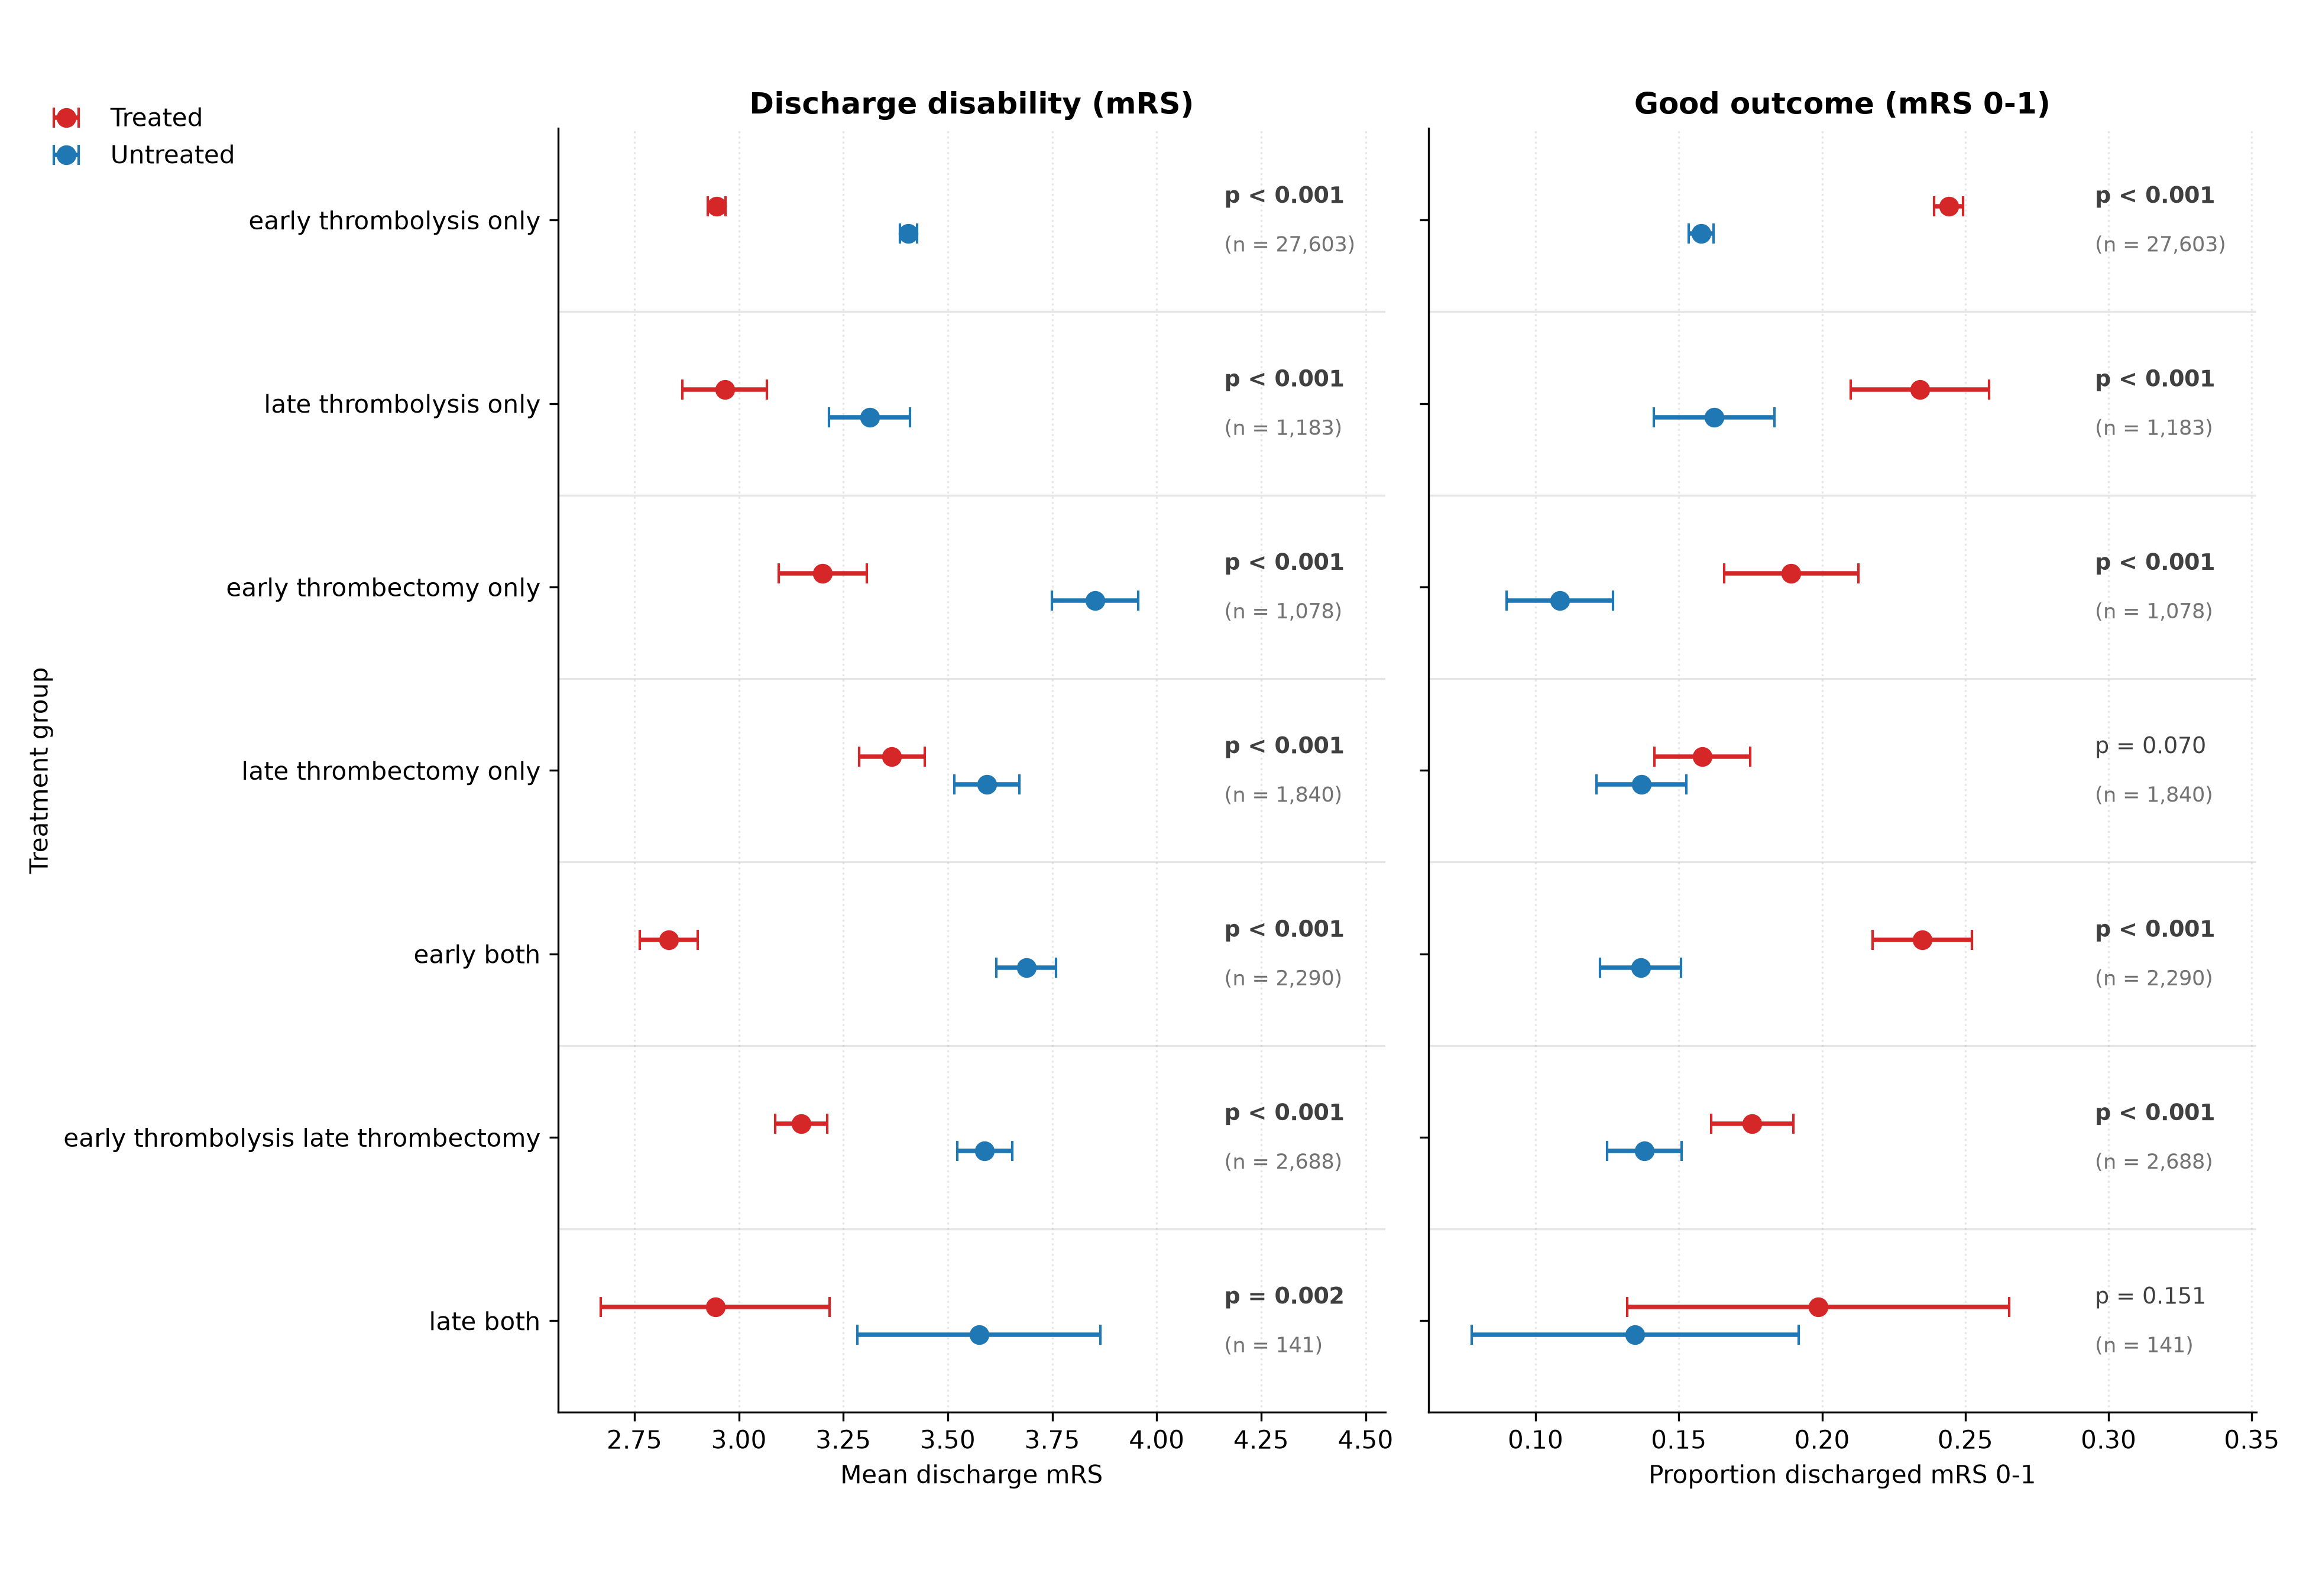
\includegraphics[width=1\linewidth]{images/treatment_effects/target_trial_emulation_mrs_1.png}
    \caption{Target trial emulation of reperfusion-treatment timing strategies and discharge functional outcomes, using matched control and treated patients. Estimated mean discharge modified Rankin Scale (mRS; left panel) and proportion achieving an outcome of mRS 0–1 (right panel) are shown for patients receiving each treatment strategy (red) and their emulated untreated comparators (blue). Strategies are defined by early ($\leq$ 270 mins from onset) or late ($>$ 270 mins from onset) intravenous thrombolysis, mechanical thrombectomy, or their combination. Points denote estimated outcomes and horizontal bars 95\% confidence intervals; p-values indicate the treated–untreated comparison within each emulated treatment group, with sample sizes shown. Lower mRS and higher mRS 0–1 proportions indicate more favourable outcomes.}
    \label{fig:target_trial_mrs_1}
\end{figure}


\begin{figure}
    \centering
    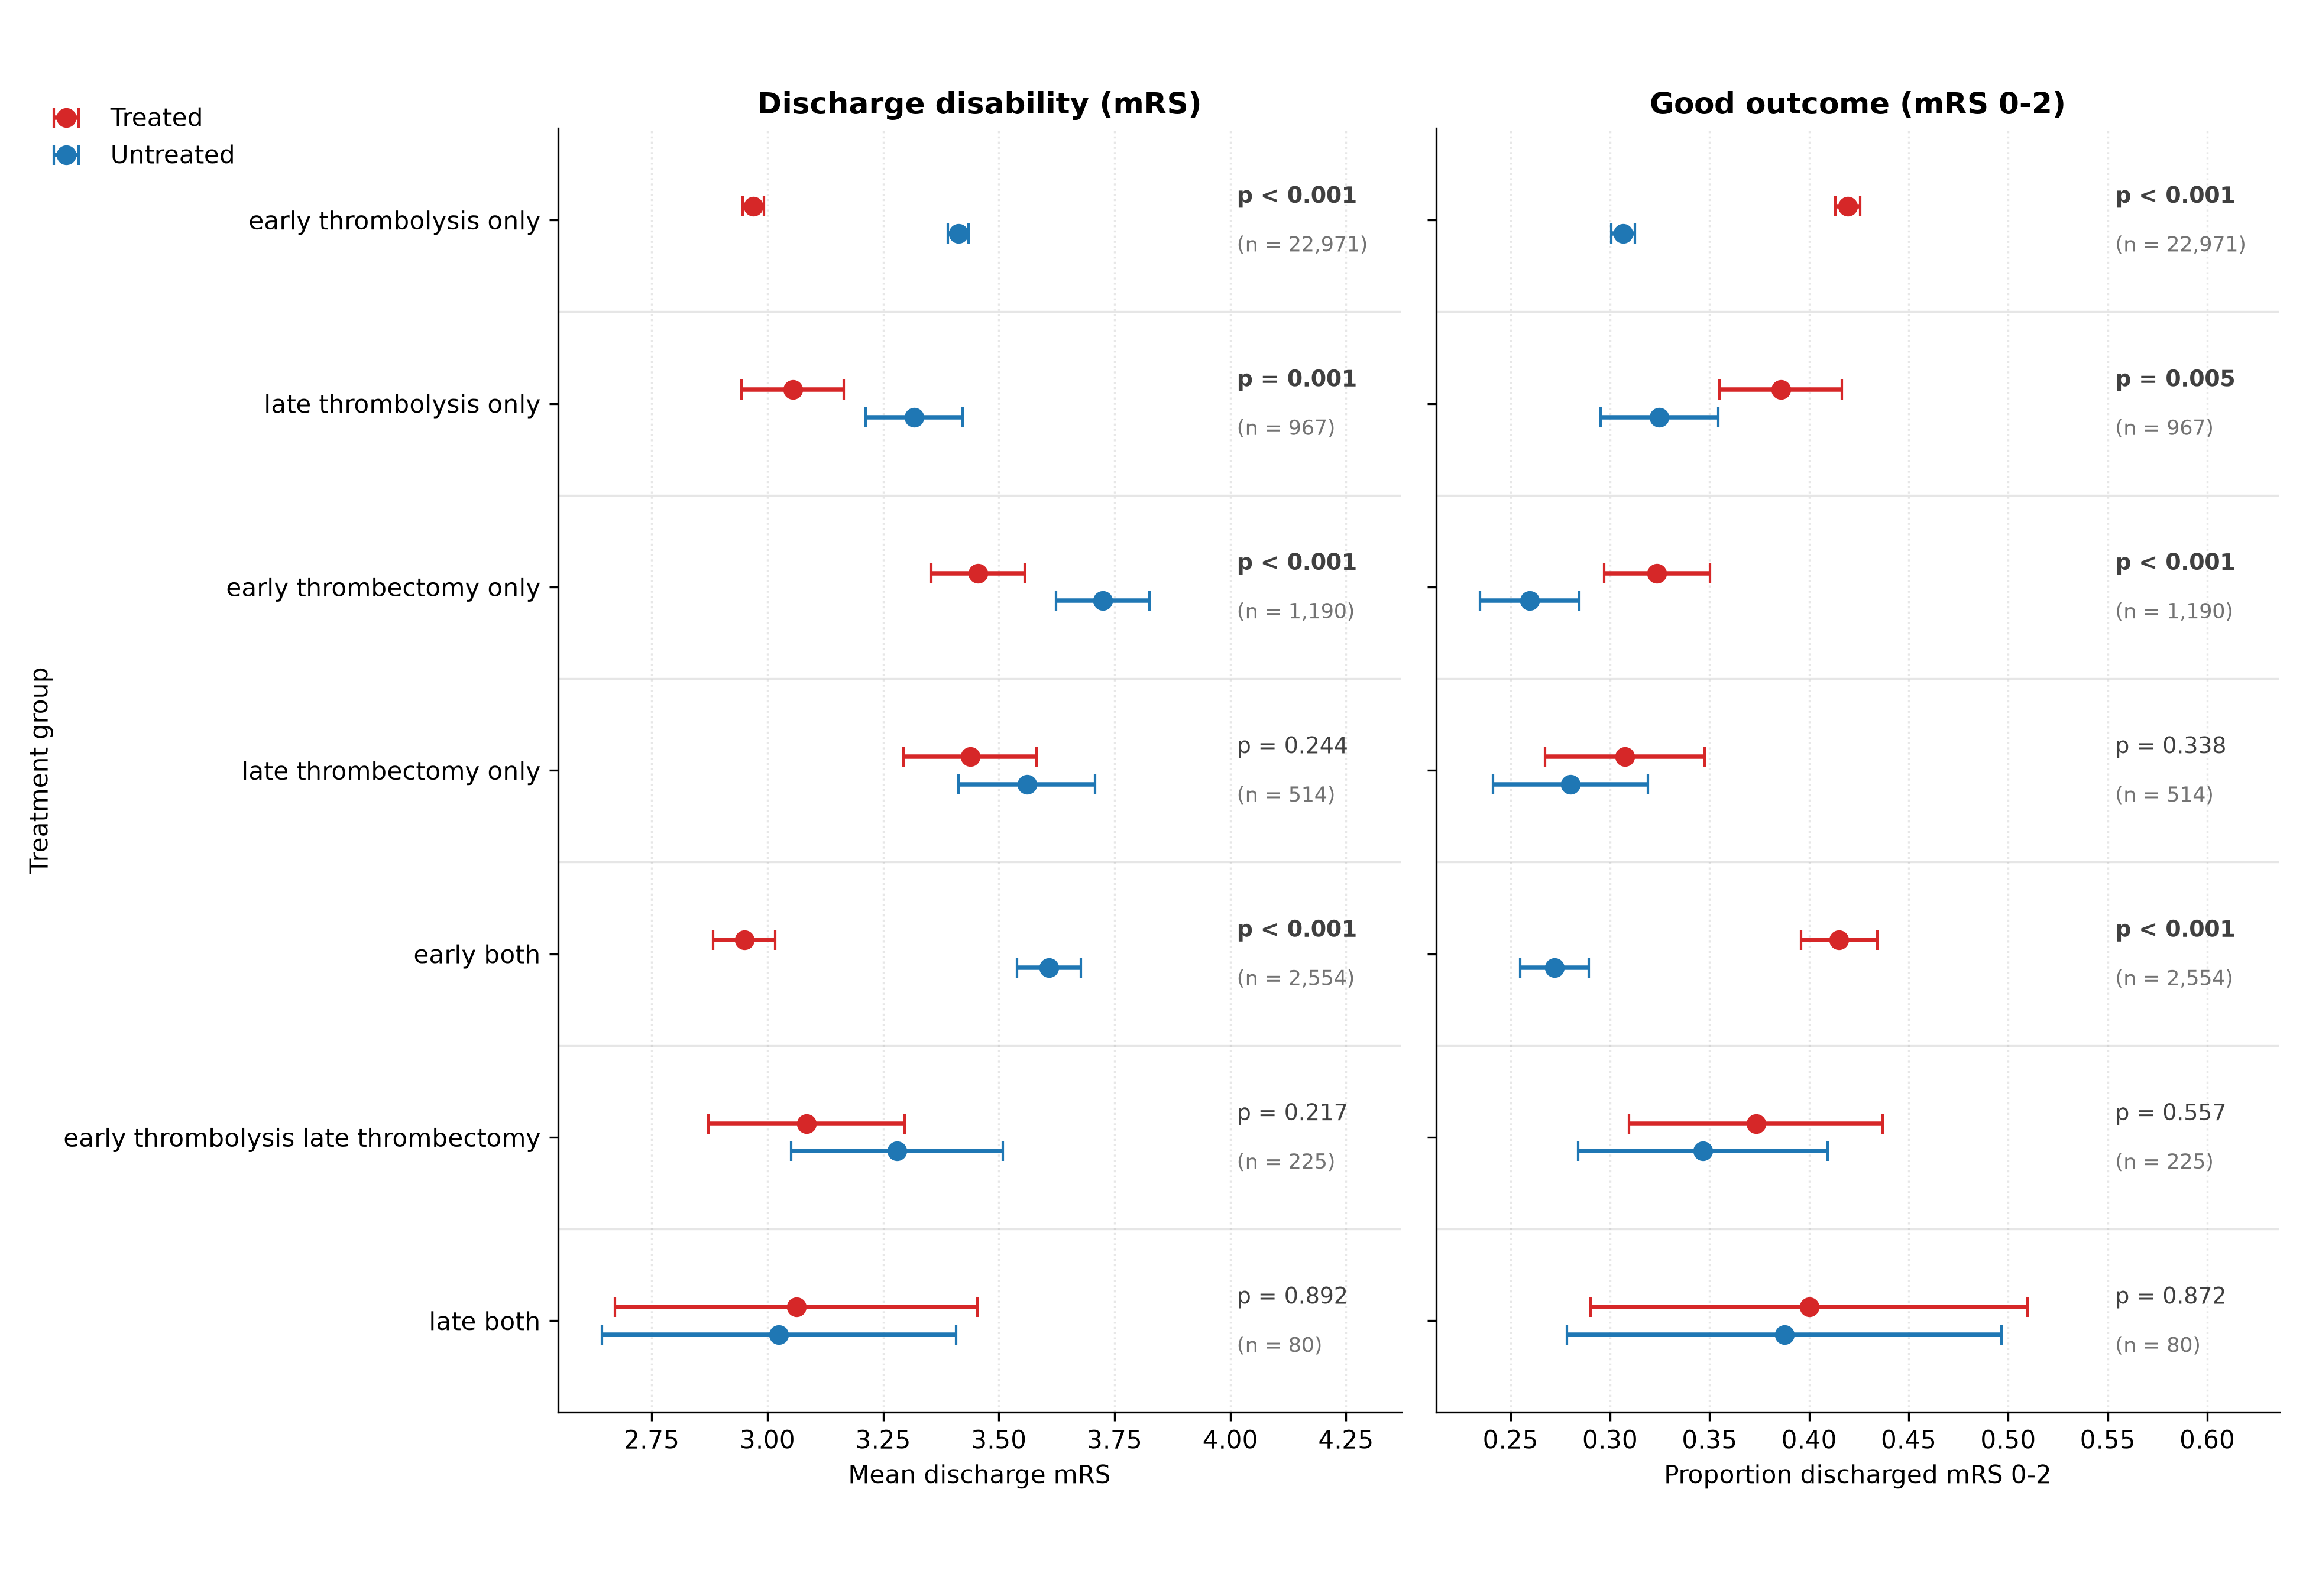
\includegraphics[width=1\linewidth]{images/treatment_effects/target_trial_emulation_mrs_2.png}
    \caption{Target trial emulation of reperfusion-treatment timing strategies and discharge functional outcomes, using matched control and treated patients. Estimated mean discharge modified Rankin Scale (mRS; left panel) and proportion achieving an outcome of mRS 0–2 (right panel) are shown for patients receiving each treatment strategy (red) and their emulated untreated comparators (blue). Strategies are defined by early ($\leq$ 270 mins from onset) or late ($>$ 270 mins from onset) intravenous thrombolysis, mechanical thrombectomy, or their combination. Points denote estimated outcomes and horizontal bars 95\% confidence intervals; p-values indicate the treated–untreated comparison within each emulated treatment group, with sample sizes shown. Lower mRS and higher mRS 0–2 proportions indicate more favourable outcomes.}
    \label{fig:target_trial_mrs_2}
\end{figure}

\begin{figure}
    \centering
    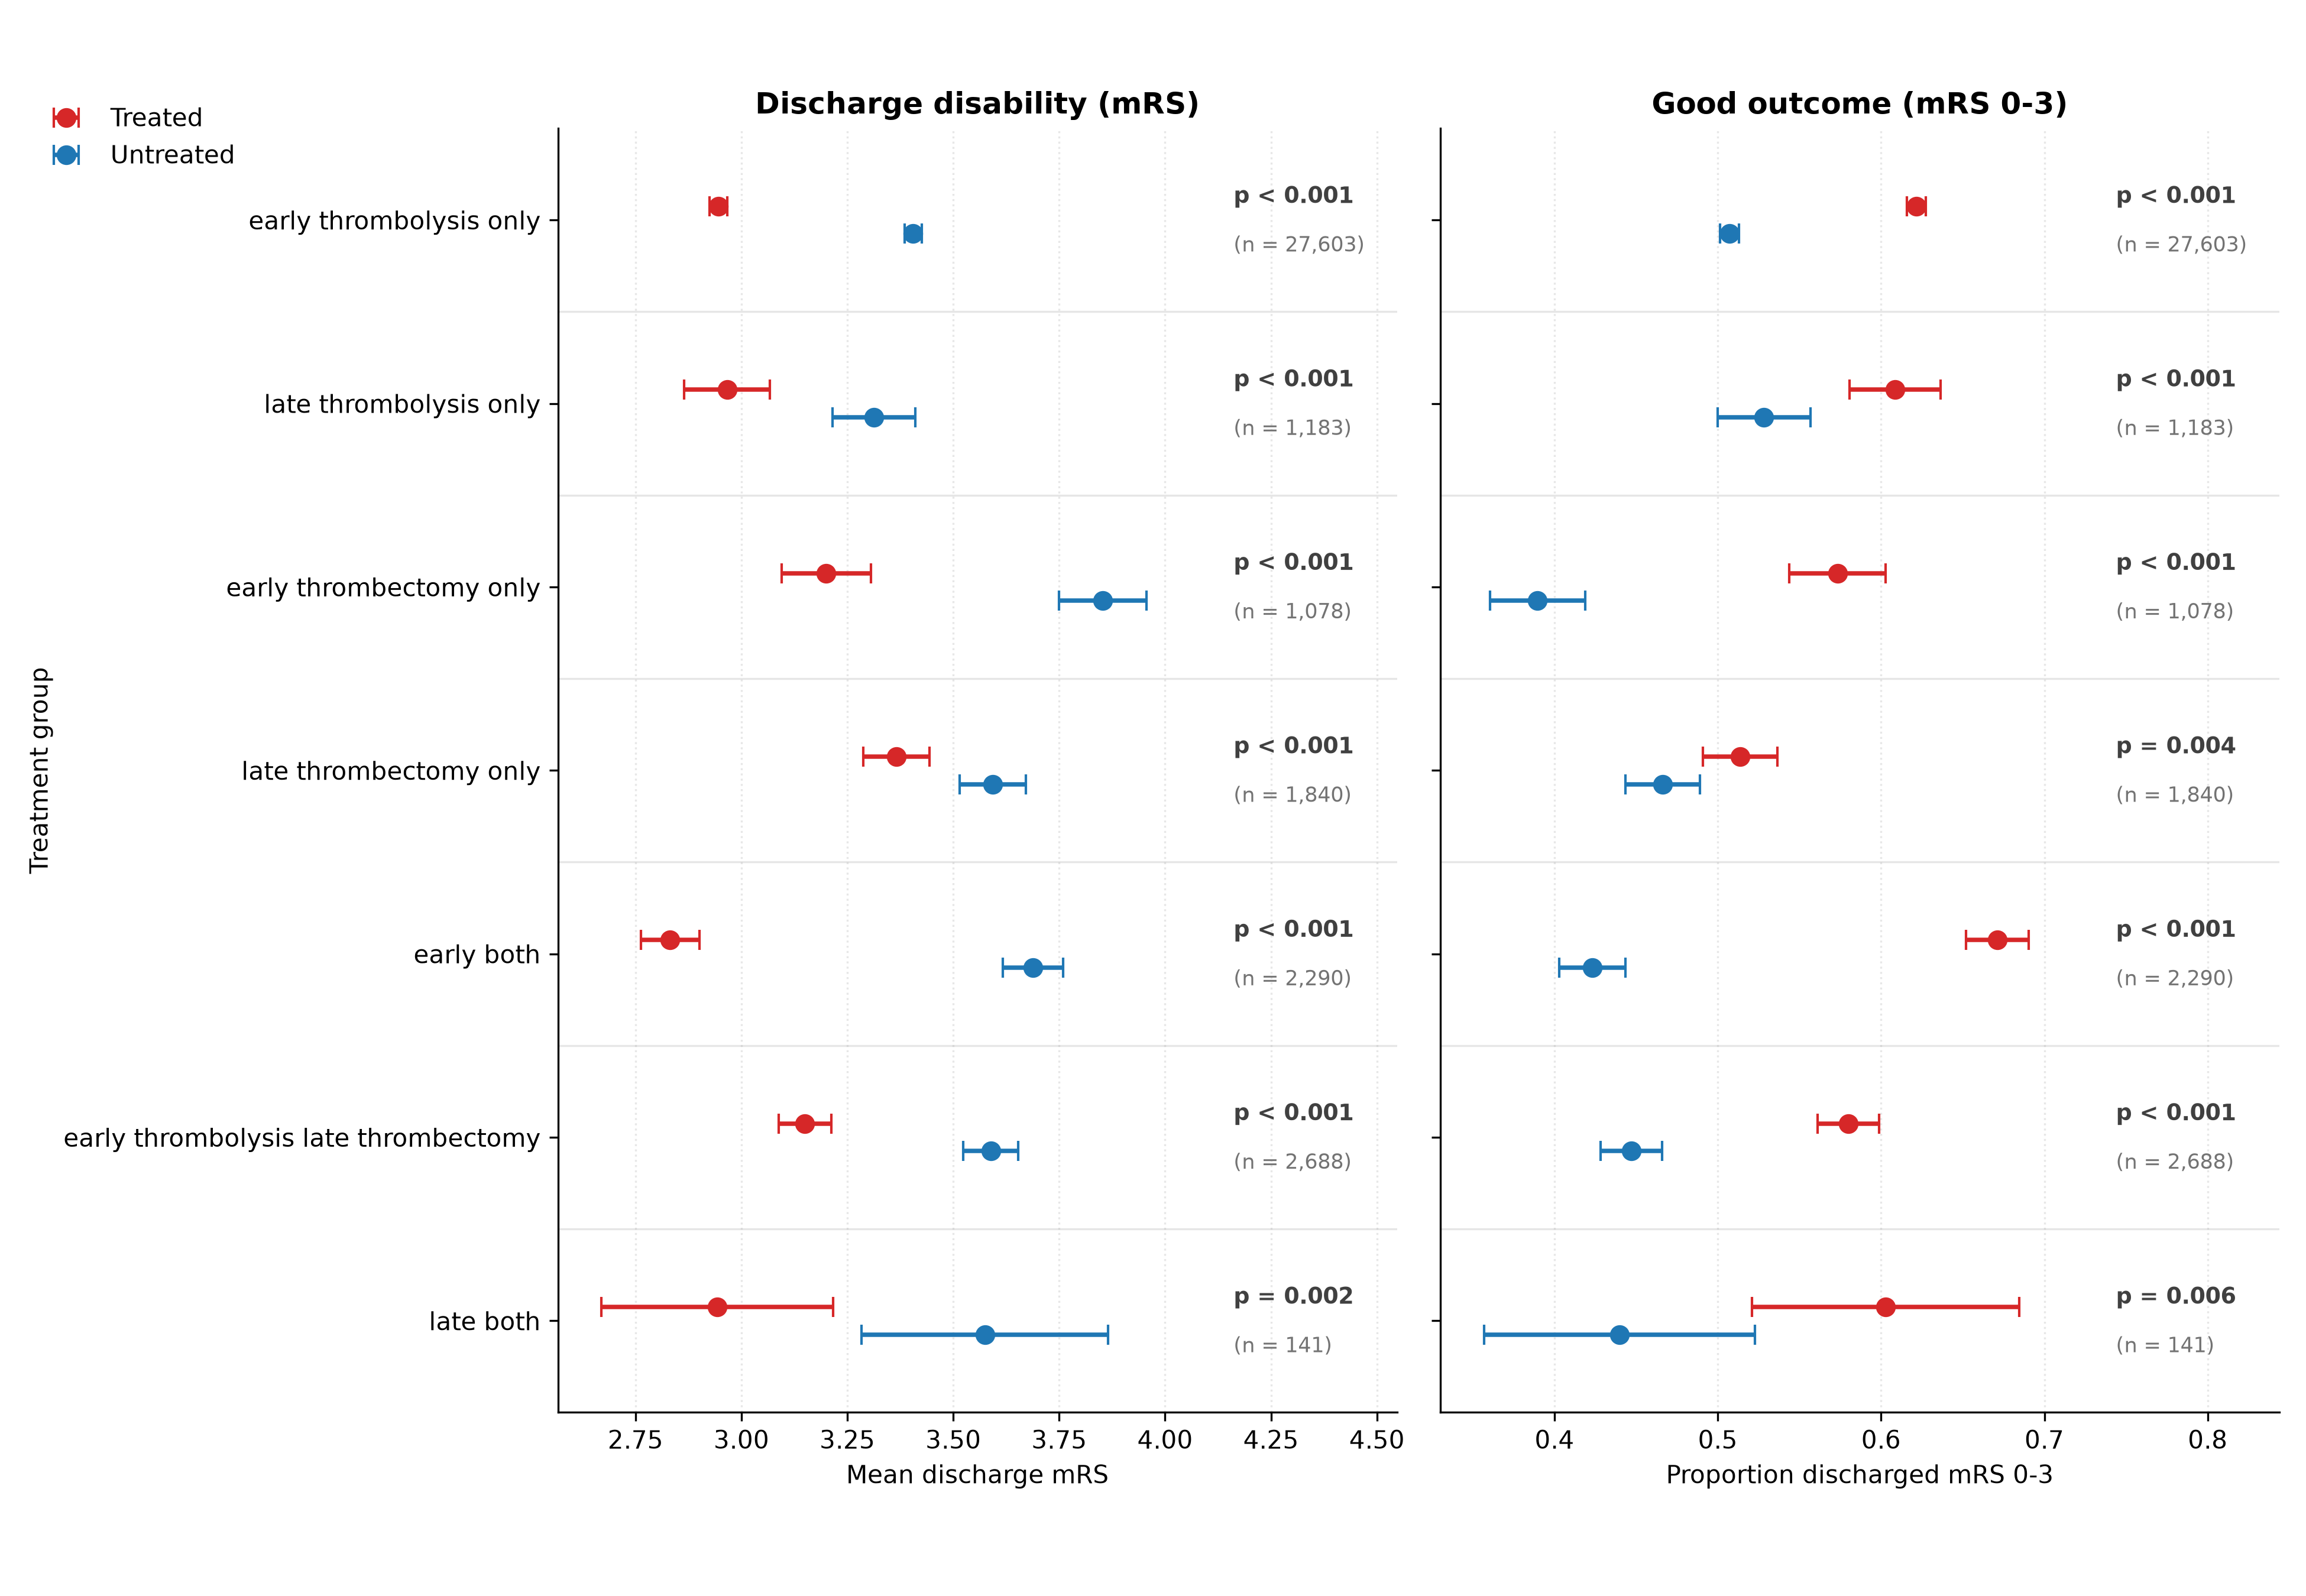
\includegraphics[width=1\linewidth]{images/treatment_effects/target_trial_emulation_mrs_3.png}
    \caption{Target trial emulation of reperfusion-treatment timing strategies and discharge functional outcomes, using matched control and treated patients. Estimated mean discharge modified Rankin Scale (mRS; left panel) and proportion achieving an outcome of mRS 0–3 (right panel) are shown for patients receiving each treatment strategy (red) and their emulated untreated comparators (blue). Strategies are defined by early ($\leq$ 270 mins from onset) or late ($>$ 270 mins from onset) intravenous thrombolysis, mechanical thrombectomy, or their combination. Points denote estimated outcomes and horizontal bars 95\% confidence intervals; p-values indicate the treated–untreated comparison within each emulated treatment group, with sample sizes shown. Lower mRS and higher mRS 0–3 proportions indicate more favourable outcomes.}
    \label{fig:target_trial_mrs_3}
\end{figure}

\begin{figure}
    \centering
    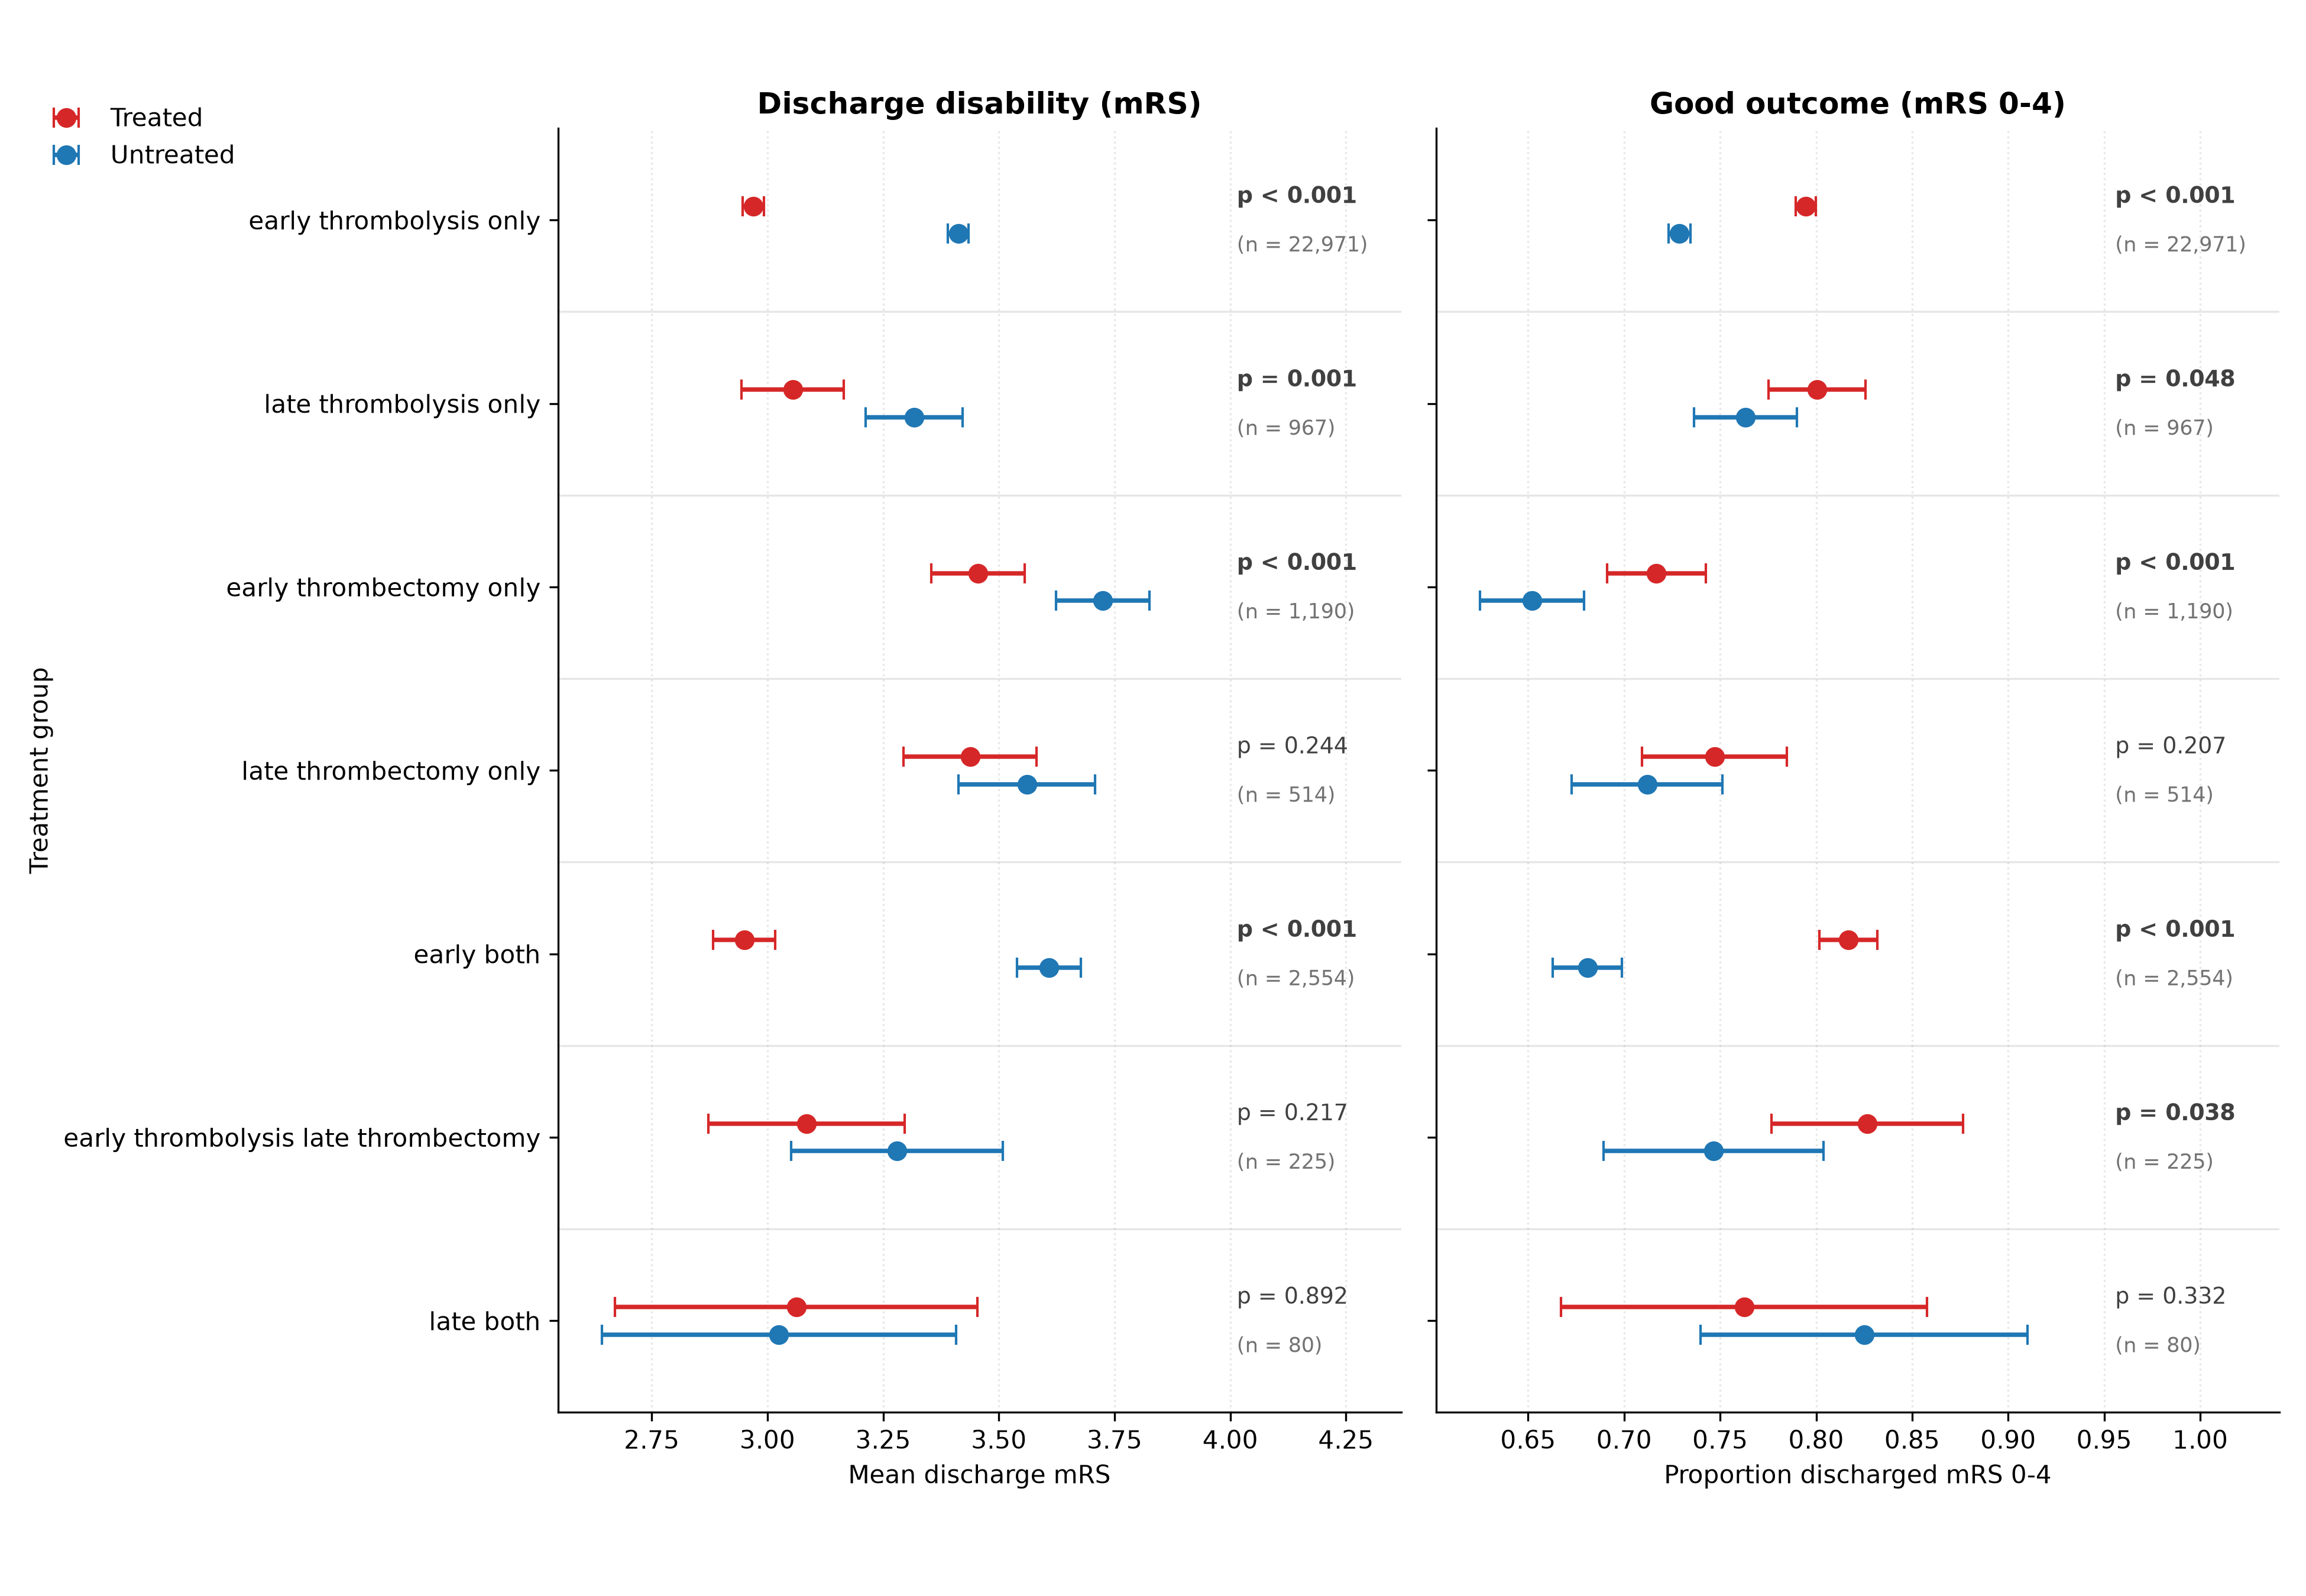
\includegraphics[width=1\linewidth]{images/treatment_effects/target_trial_emulation_mrs_4.png}
    \caption{Target trial emulation of reperfusion-treatment timing strategies and discharge functional outcomes, using matched control and treated patients. Estimated mean discharge modified Rankin Scale (mRS; left panel) and proportion achieving an outcome of mRS 0–4 (right panel) are shown for patients receiving each treatment strategy (red) and their emulated untreated comparators (blue). Strategies are defined by early ($\leq$ 270 mins from onset) or late ($>$ 270 mins from onset) intravenous thrombolysis, mechanical thrombectomy, or their combination. Points denote estimated outcomes and horizontal bars 95\% confidence intervals; p-values indicate the treated–untreated comparison within each emulated treatment group, with sample sizes shown. Lower mRS and higher mRS 0–4 proportions indicate more favourable outcomes.}
    \label{fig:target_trial_mrs_4}
\end{figure}

\begin{figure}
    \centering
    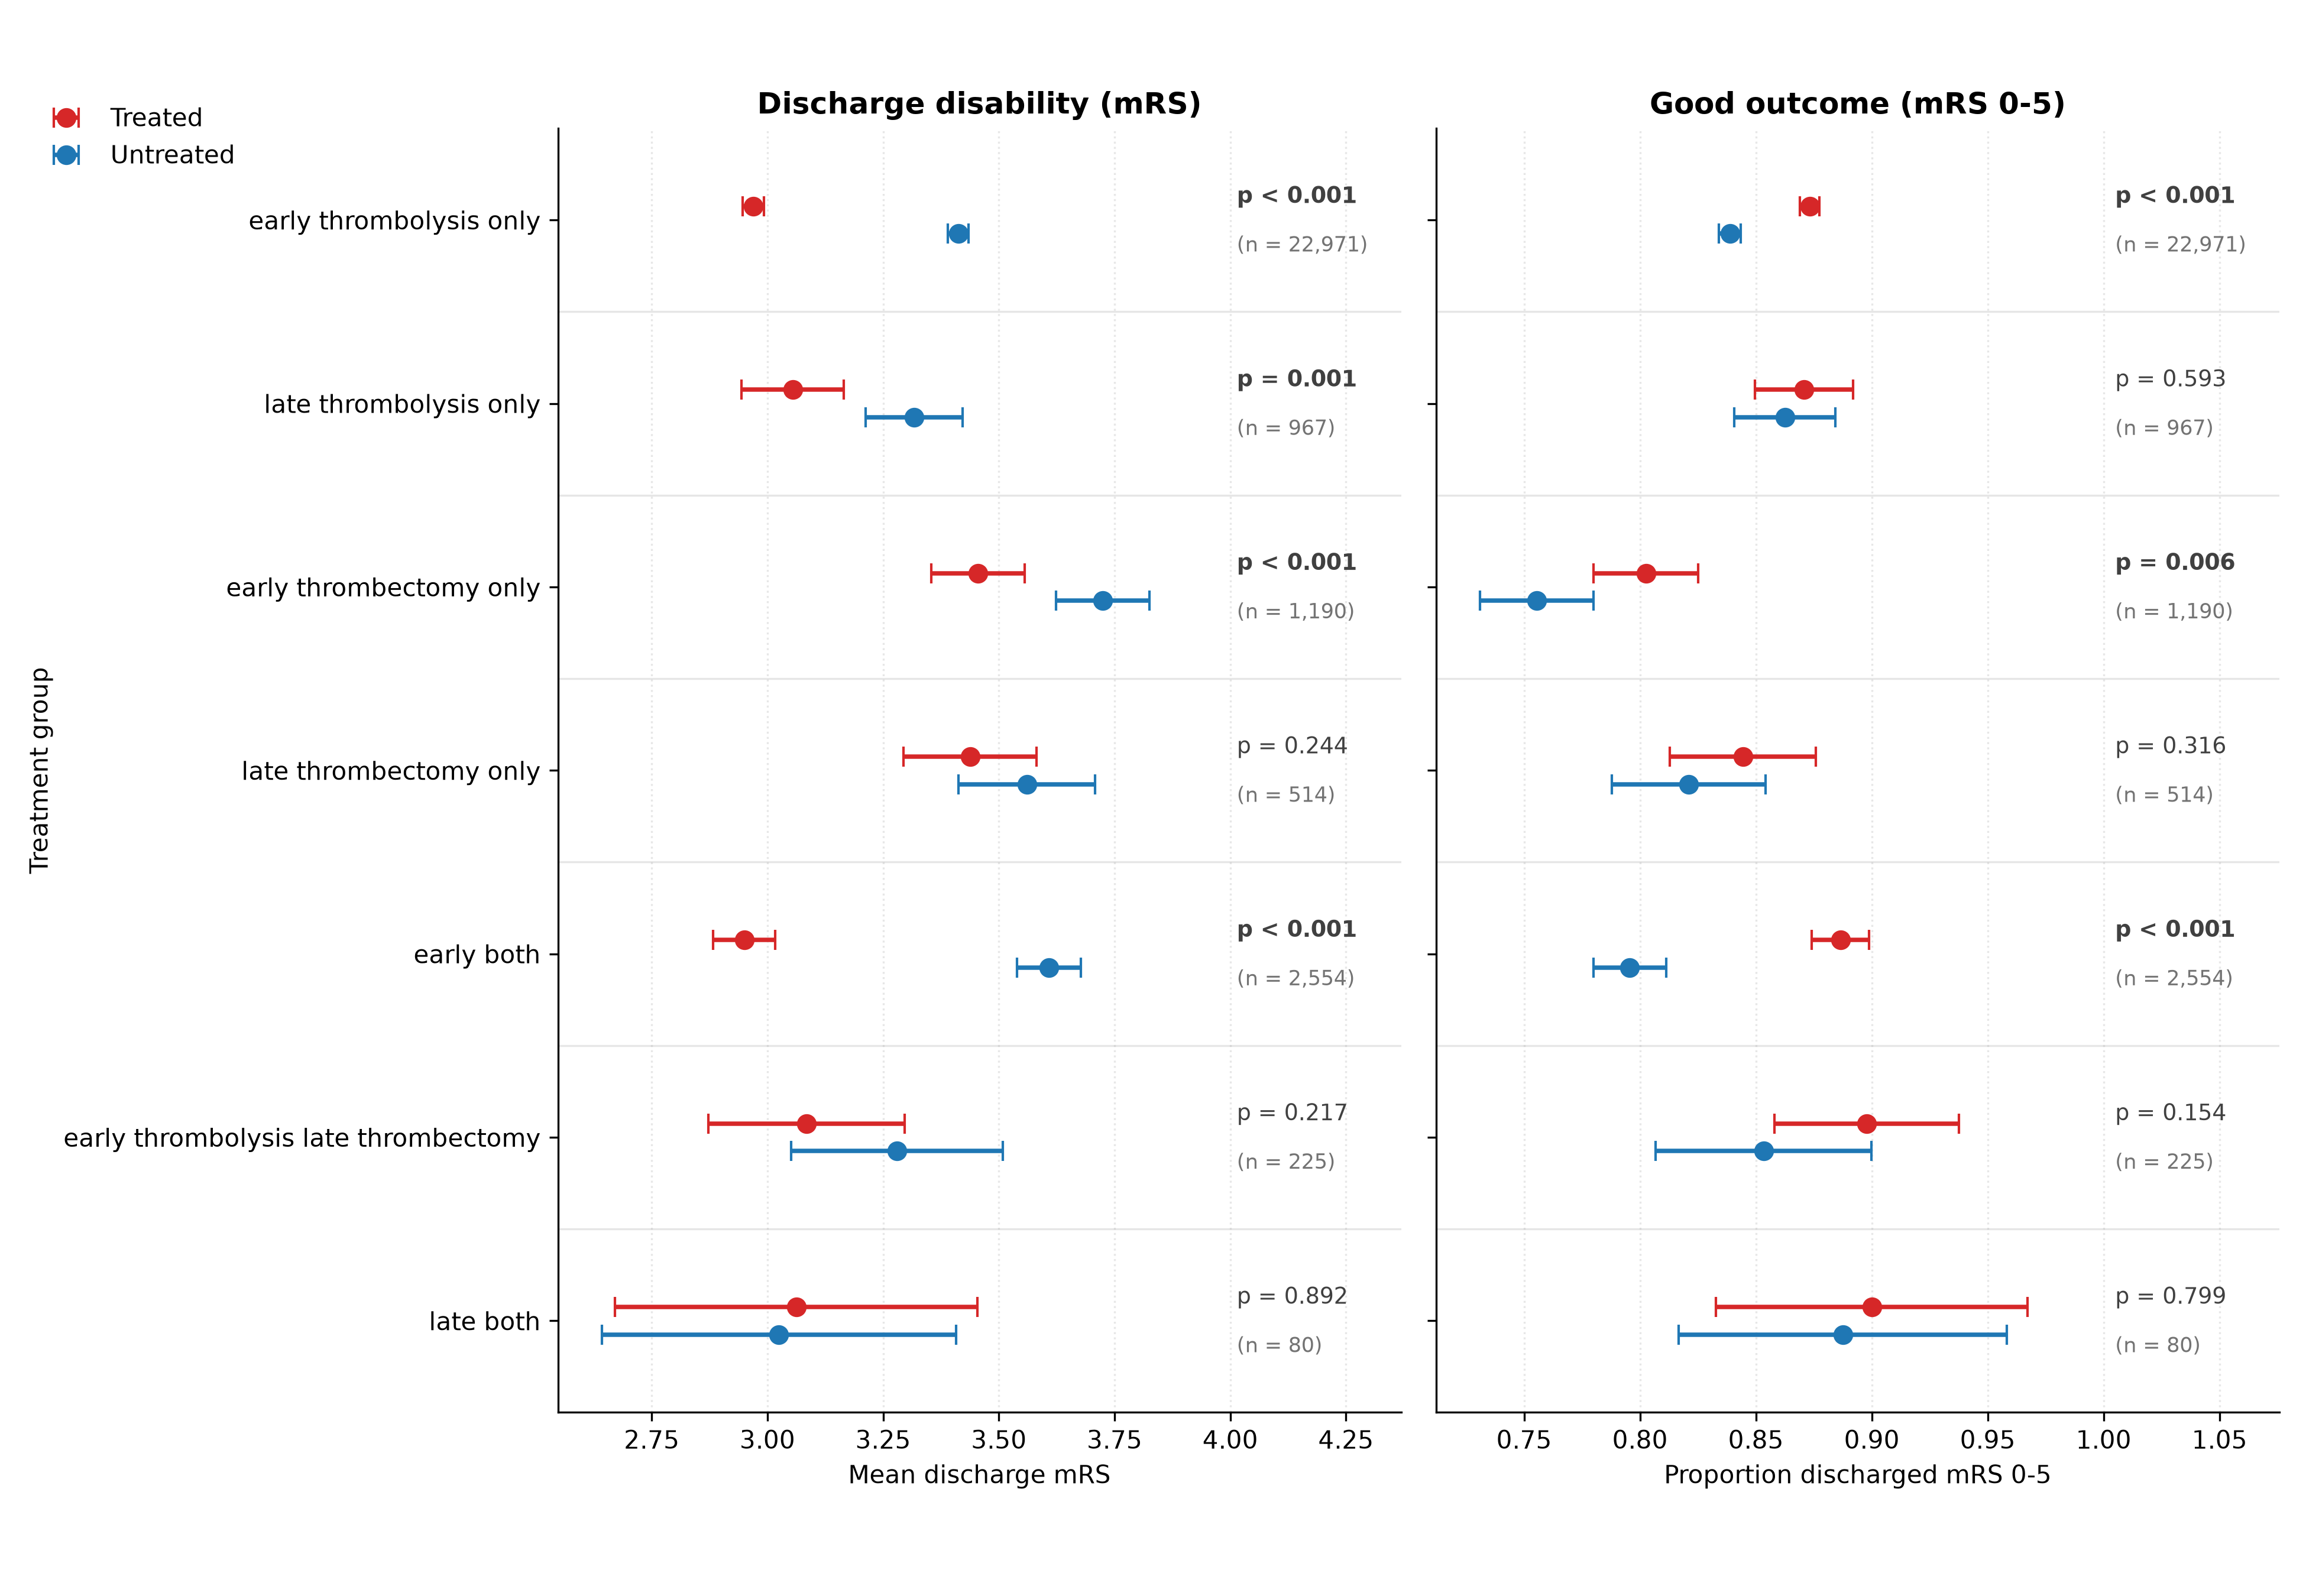
\includegraphics[width=1\linewidth]{images/treatment_effects/target_trial_emulation_mrs_5.png}
    \caption{Target trial emulation of reperfusion-treatment timing strategies and discharge functional outcomes, using matched control and treated patients. Estimated mean discharge modified Rankin Scale (mRS; left panel) and proportion achieving an outcome of mRS 0–5 (survival, right panel) are shown for patients receiving each treatment strategy (red) and their emulated untreated comparators (blue). Strategies are defined by early ($\leq$ 270 mins from onset) or late ($>$ 270 mins from onset) intravenous thrombolysis, mechanical thrombectomy, or their combination. Points denote estimated outcomes and horizontal bars 95\% confidence intervals; p-values indicate the treated–untreated comparison within each emulated treatment group, with sample sizes shown. Lower mRS and higher mRS 0–5 proportions indicate more favourable outcomes.}
    \label{fig:target_trial_mrs_5}
\end{figure}

% ------------------------------------------------------------------------------------

\newpage

\subsection{S-Learner}

Figure \ref{fig:s_learner_benefit} shows treatment effect estimates, estimated using an XG-Boost S-Learner and counterfactual modelling, for achieving each possible mRS threshold. Treatment effects are shown as log odds ratio (treated vs. untreated) in obtaining a favourable outcome. Treatment type and speed (early vs late, using a 270 min onset-to-treatment threshold) were coded as a categorical value for this model.

%%%%%%%%%%%%%%%%%%%%%%%%%%%%%%%%%%%%%%%%%%

\begin{figure}
    \centering
    
    % Top left
    \begin{subfigure}{0.48\textwidth}
        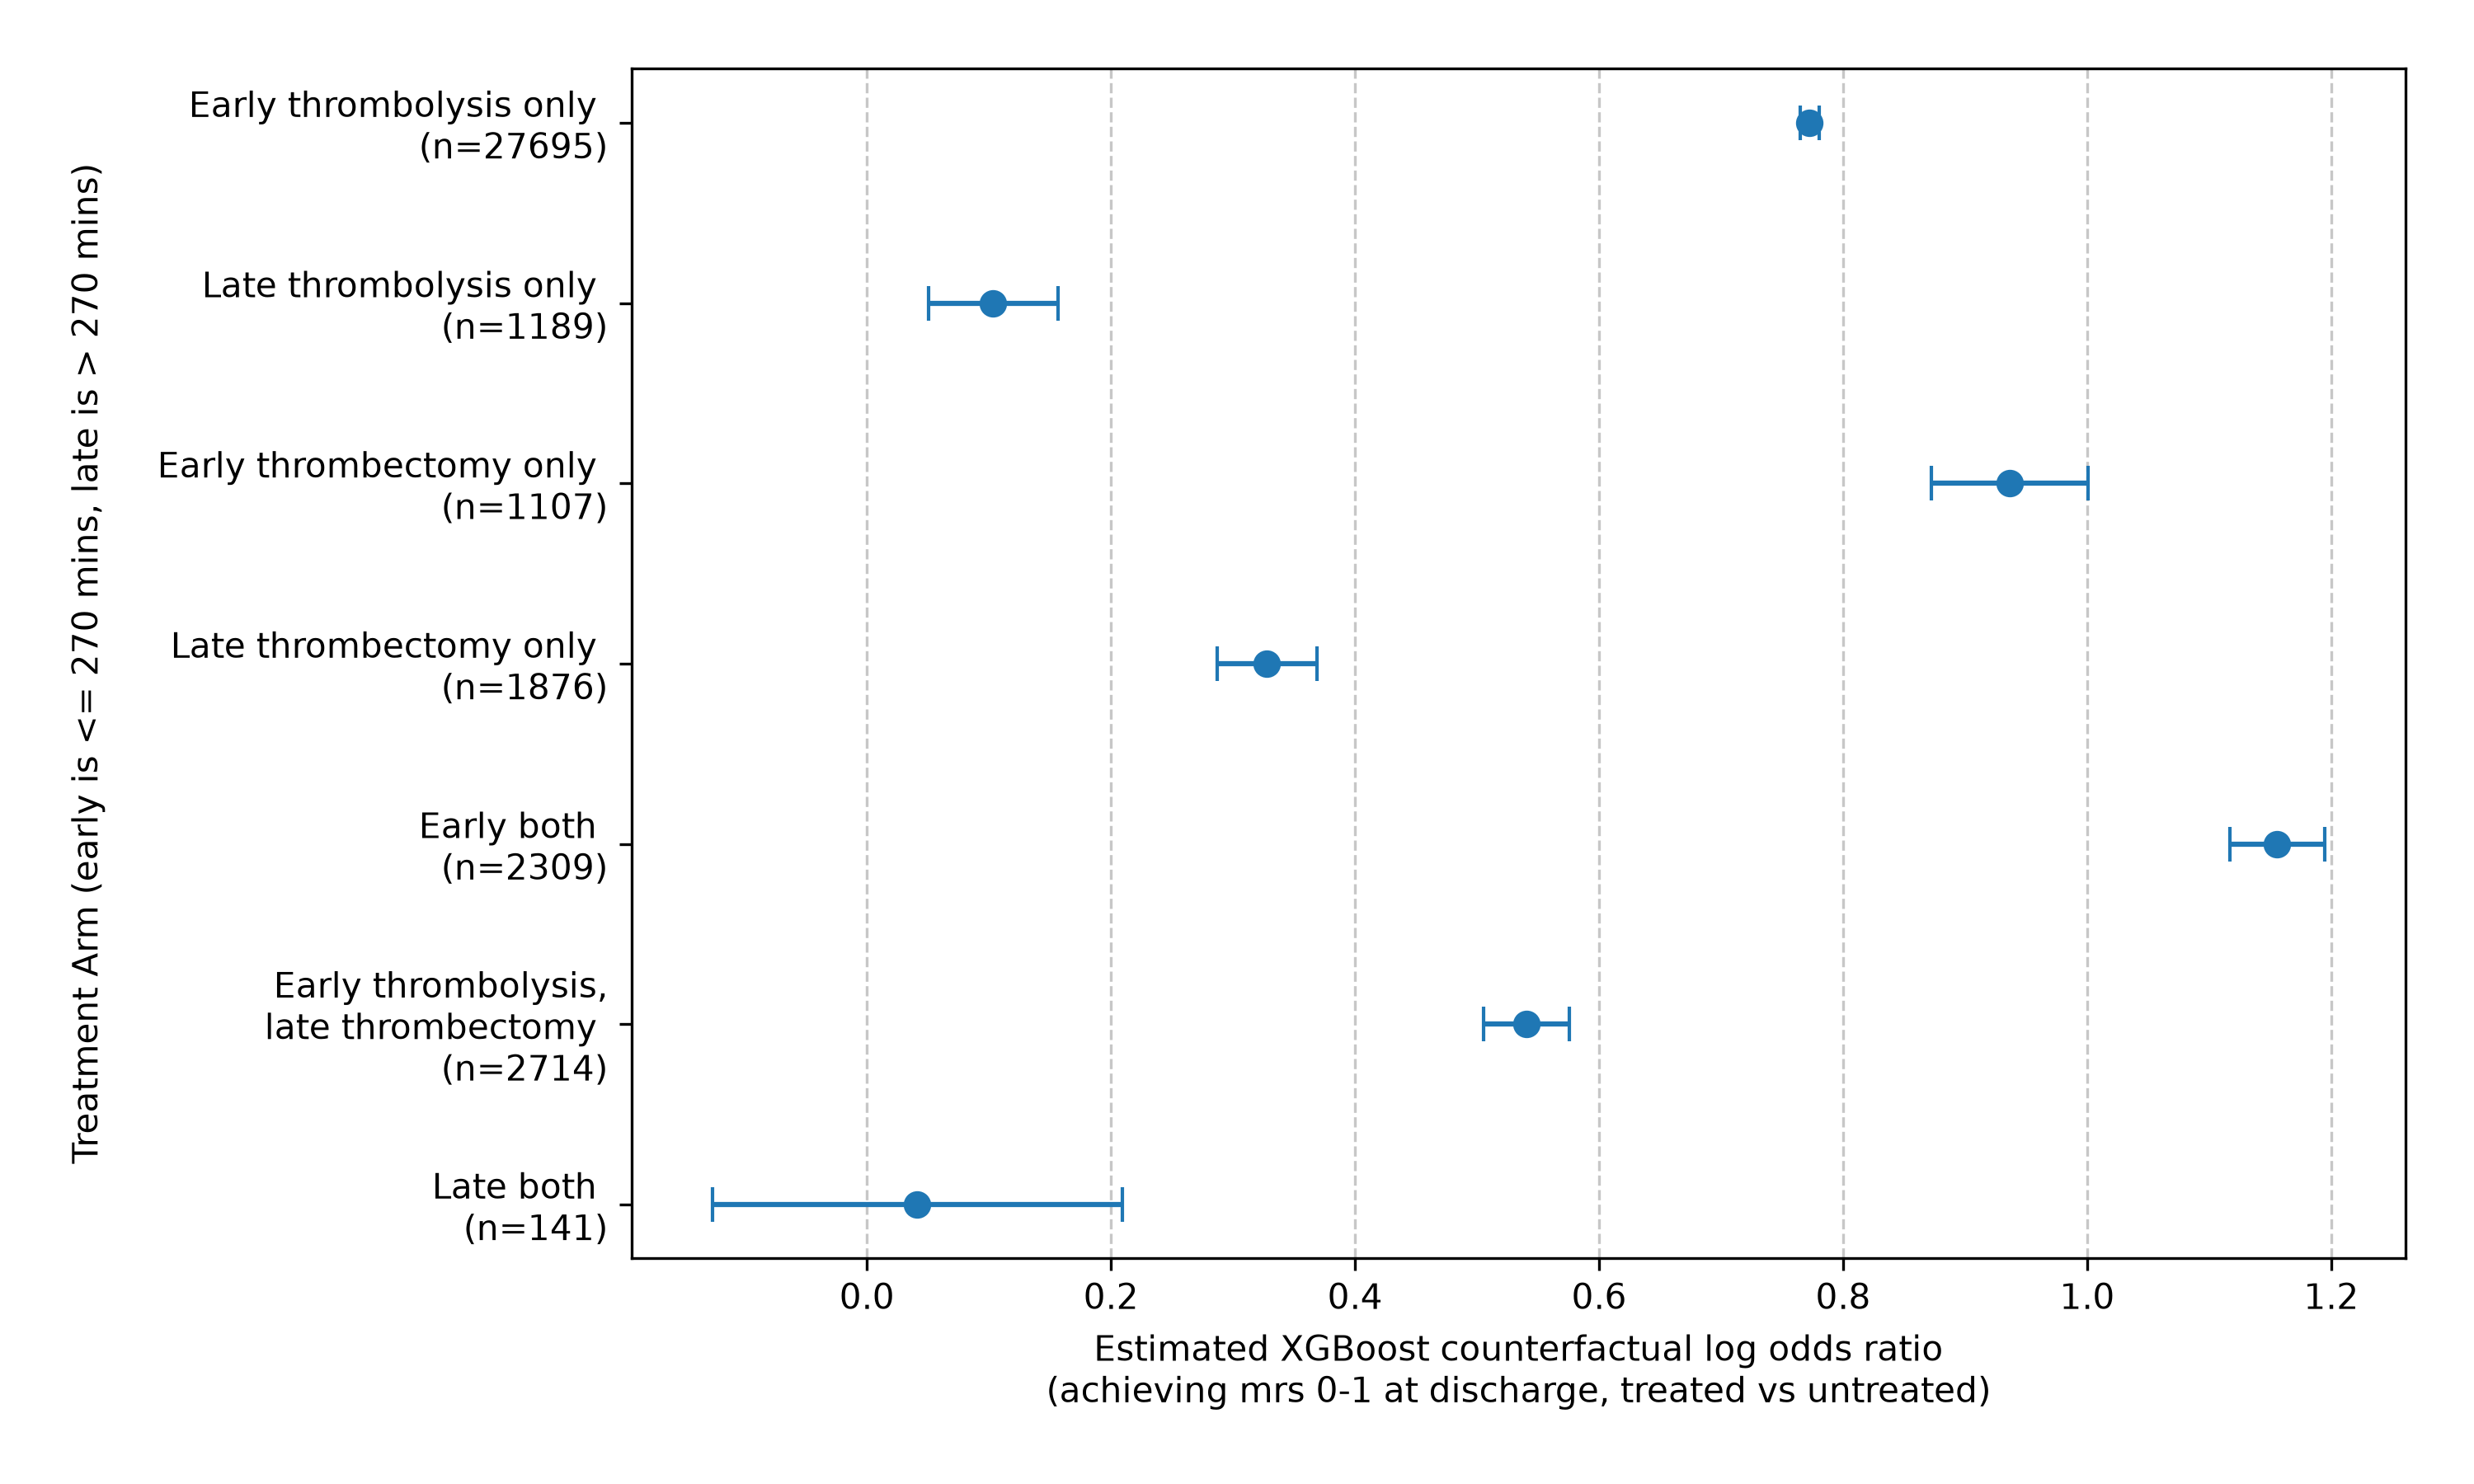
\includegraphics[width=\linewidth]{images/treatment_effects/xgboost_counterfactual_cate_log_odds_estimates_1.png}
        %\caption{}
        \label{fig:top-left}
    \end{subfigure}
    \hfill % Adds flexible horizontal spacing
    % top right image 
    \begin{subfigure}{0.48\textwidth}
        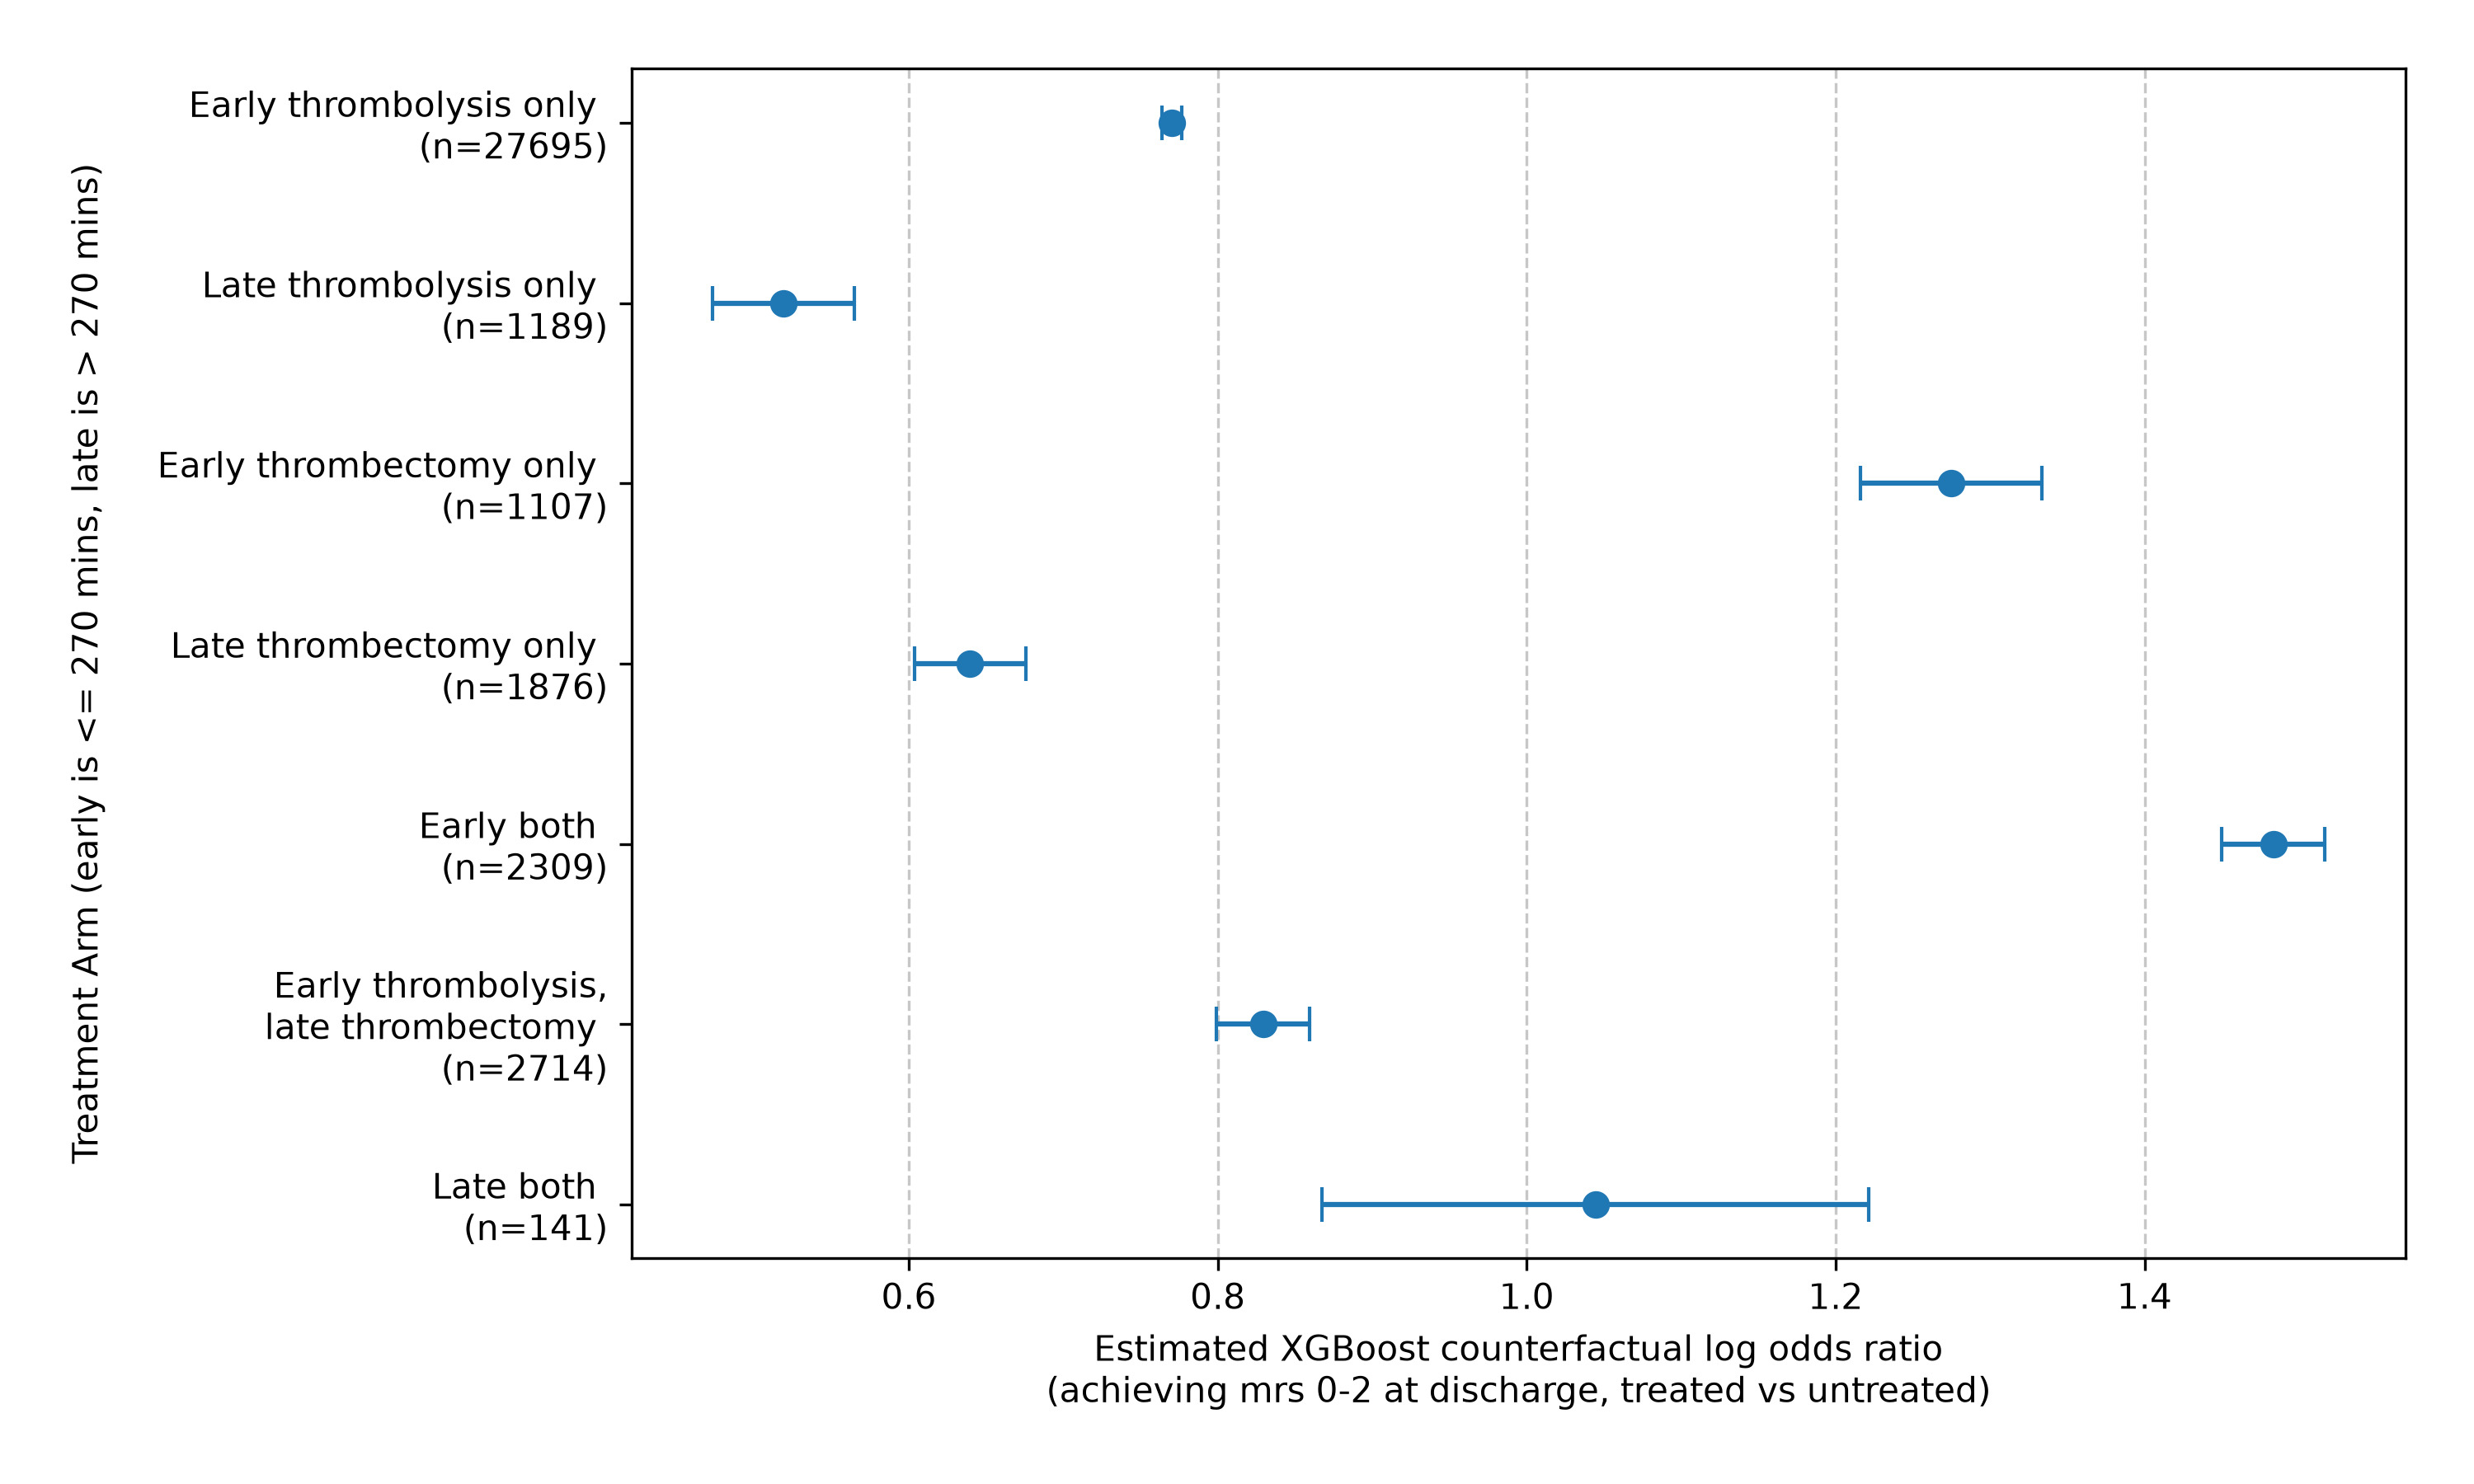
\includegraphics[width=\linewidth]{images/treatment_effects/xgboost_counterfactual_cate_log_odds_estimates_2.png}
        %\caption{}
        \label{fig:bottom-left}
    \end{subfigure}

    \vspace{0.5cm} % Optional vertical space between rows

    % Center left image
    \begin{subfigure}{0.48\textwidth}
        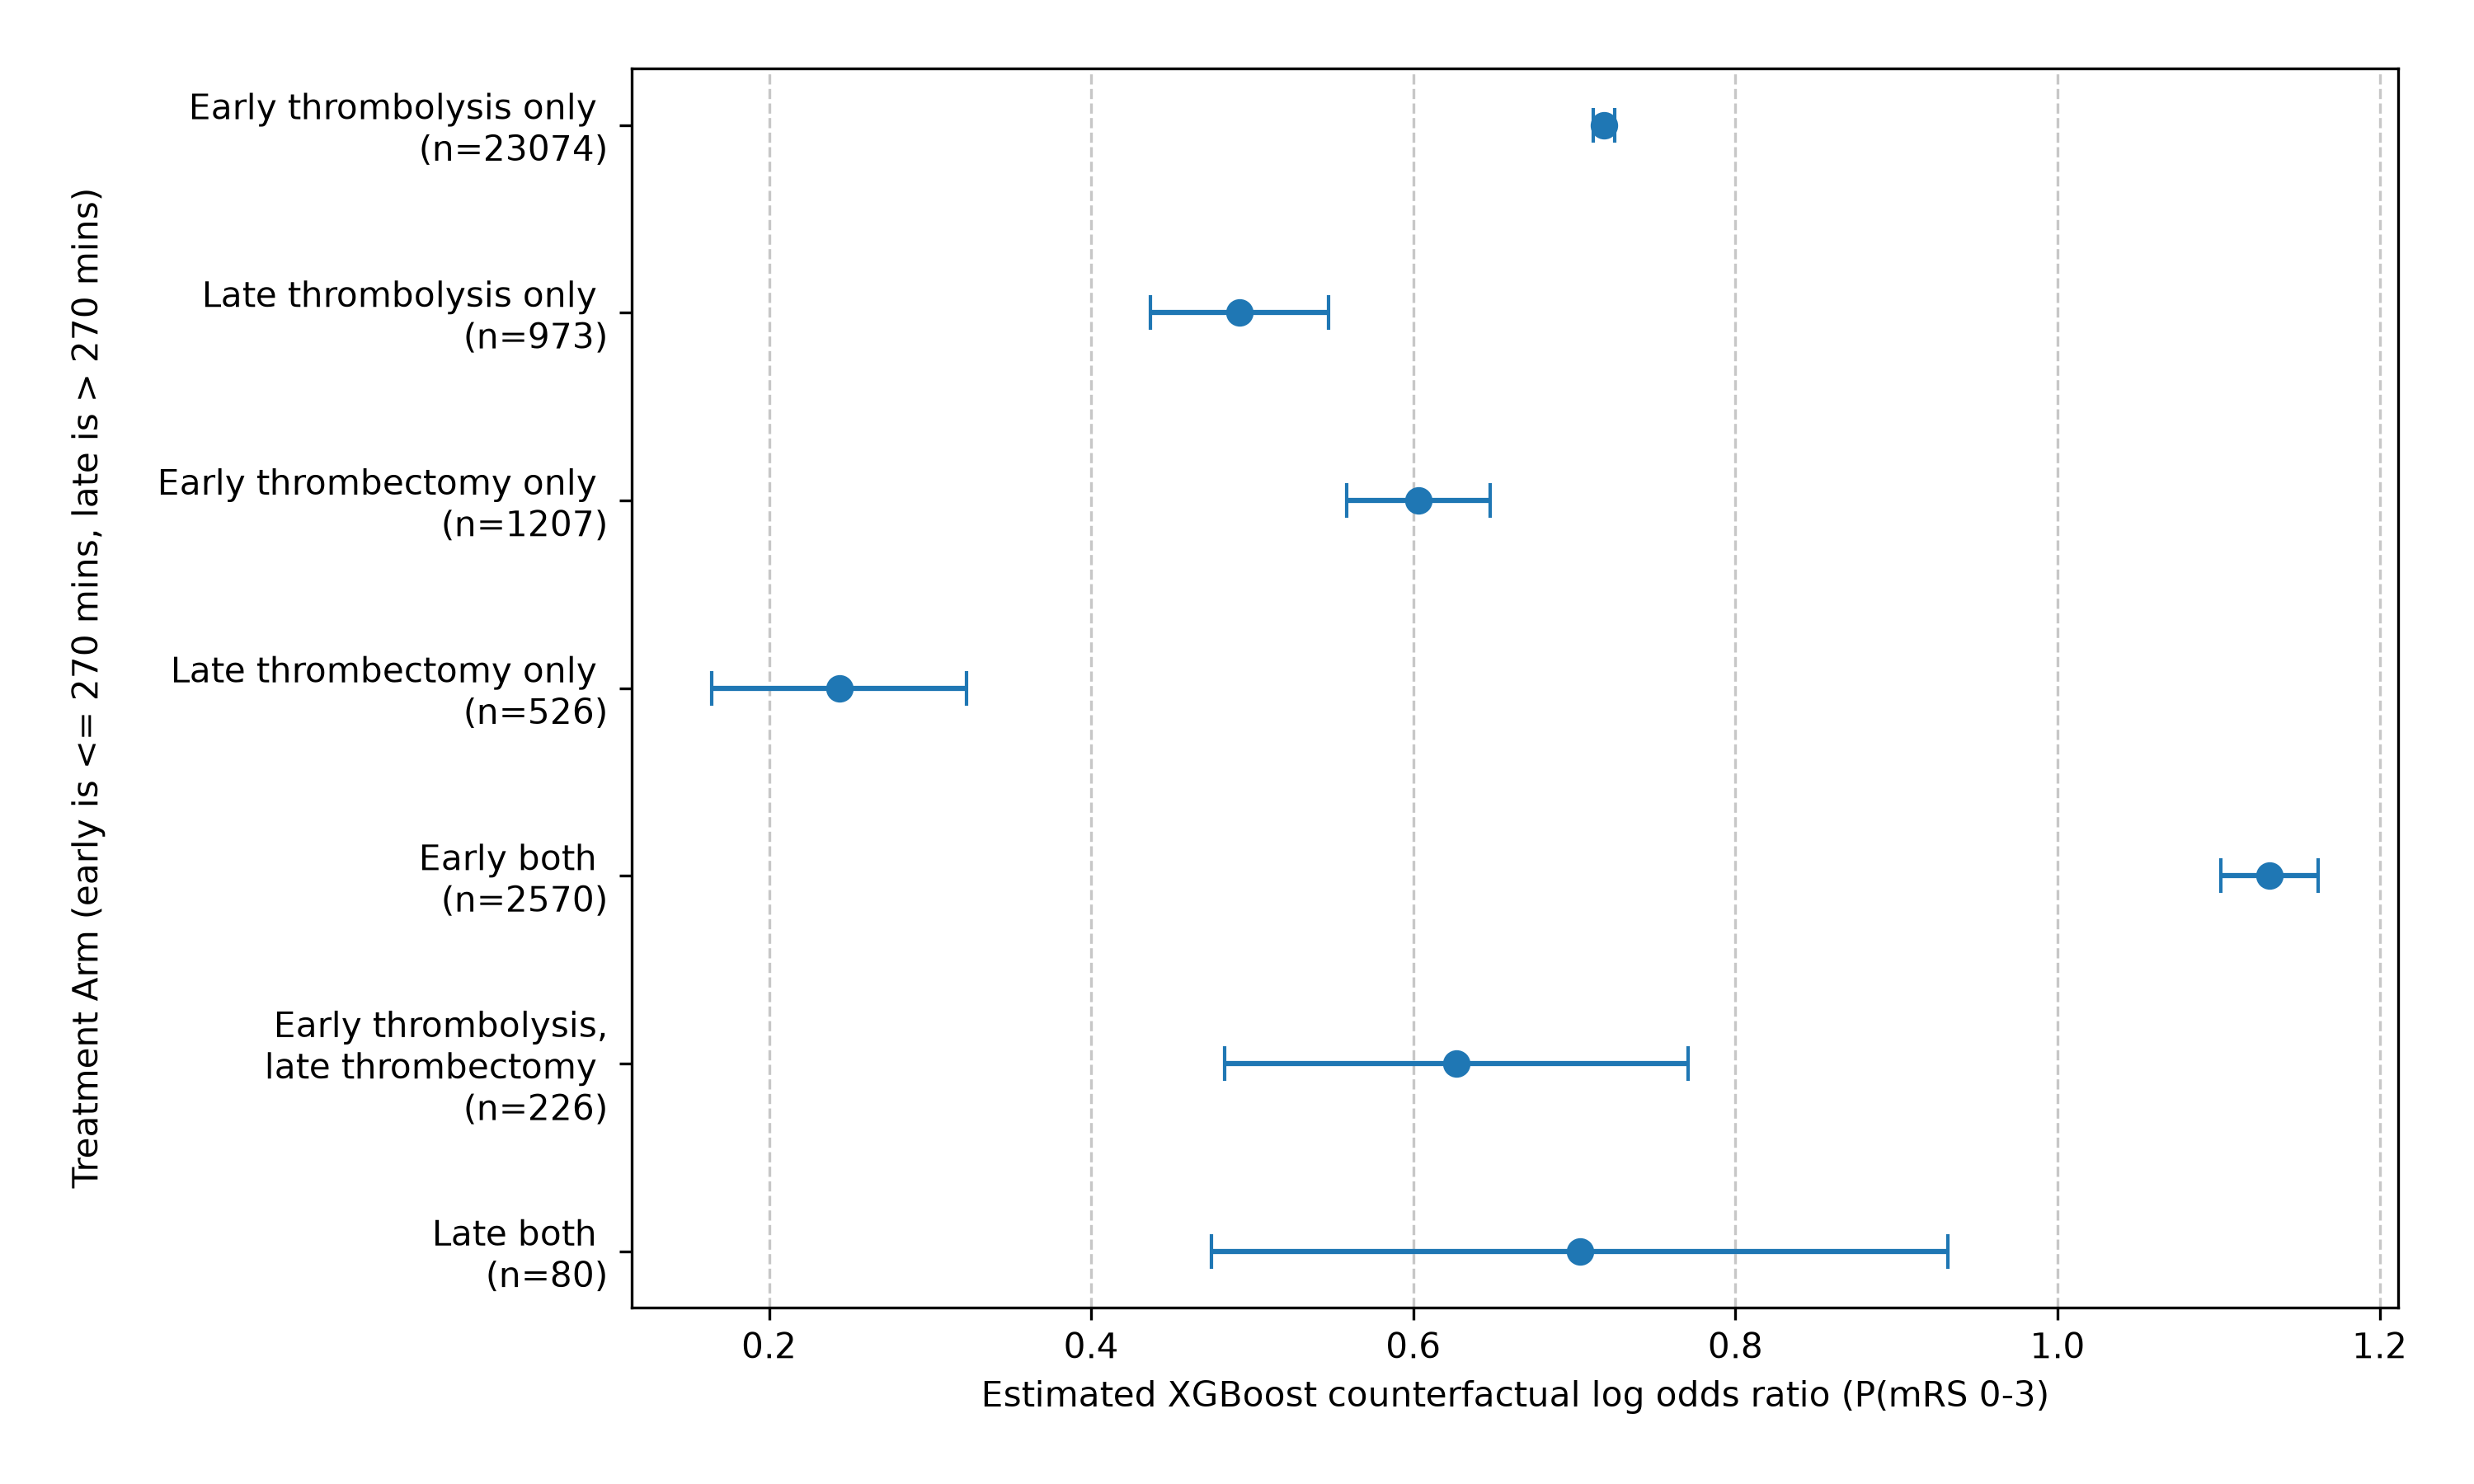
\includegraphics[width=\linewidth]{images/treatment_effects/xgboost_counterfactual_cate_log_odds_estimates_3}
        %\caption{}
        \label{fig:centre-left}
    \end{subfigure}
    \hfill % Adds flexible horizontal spacing
    % Centre right image 
    \begin{subfigure}{0.48\textwidth}
        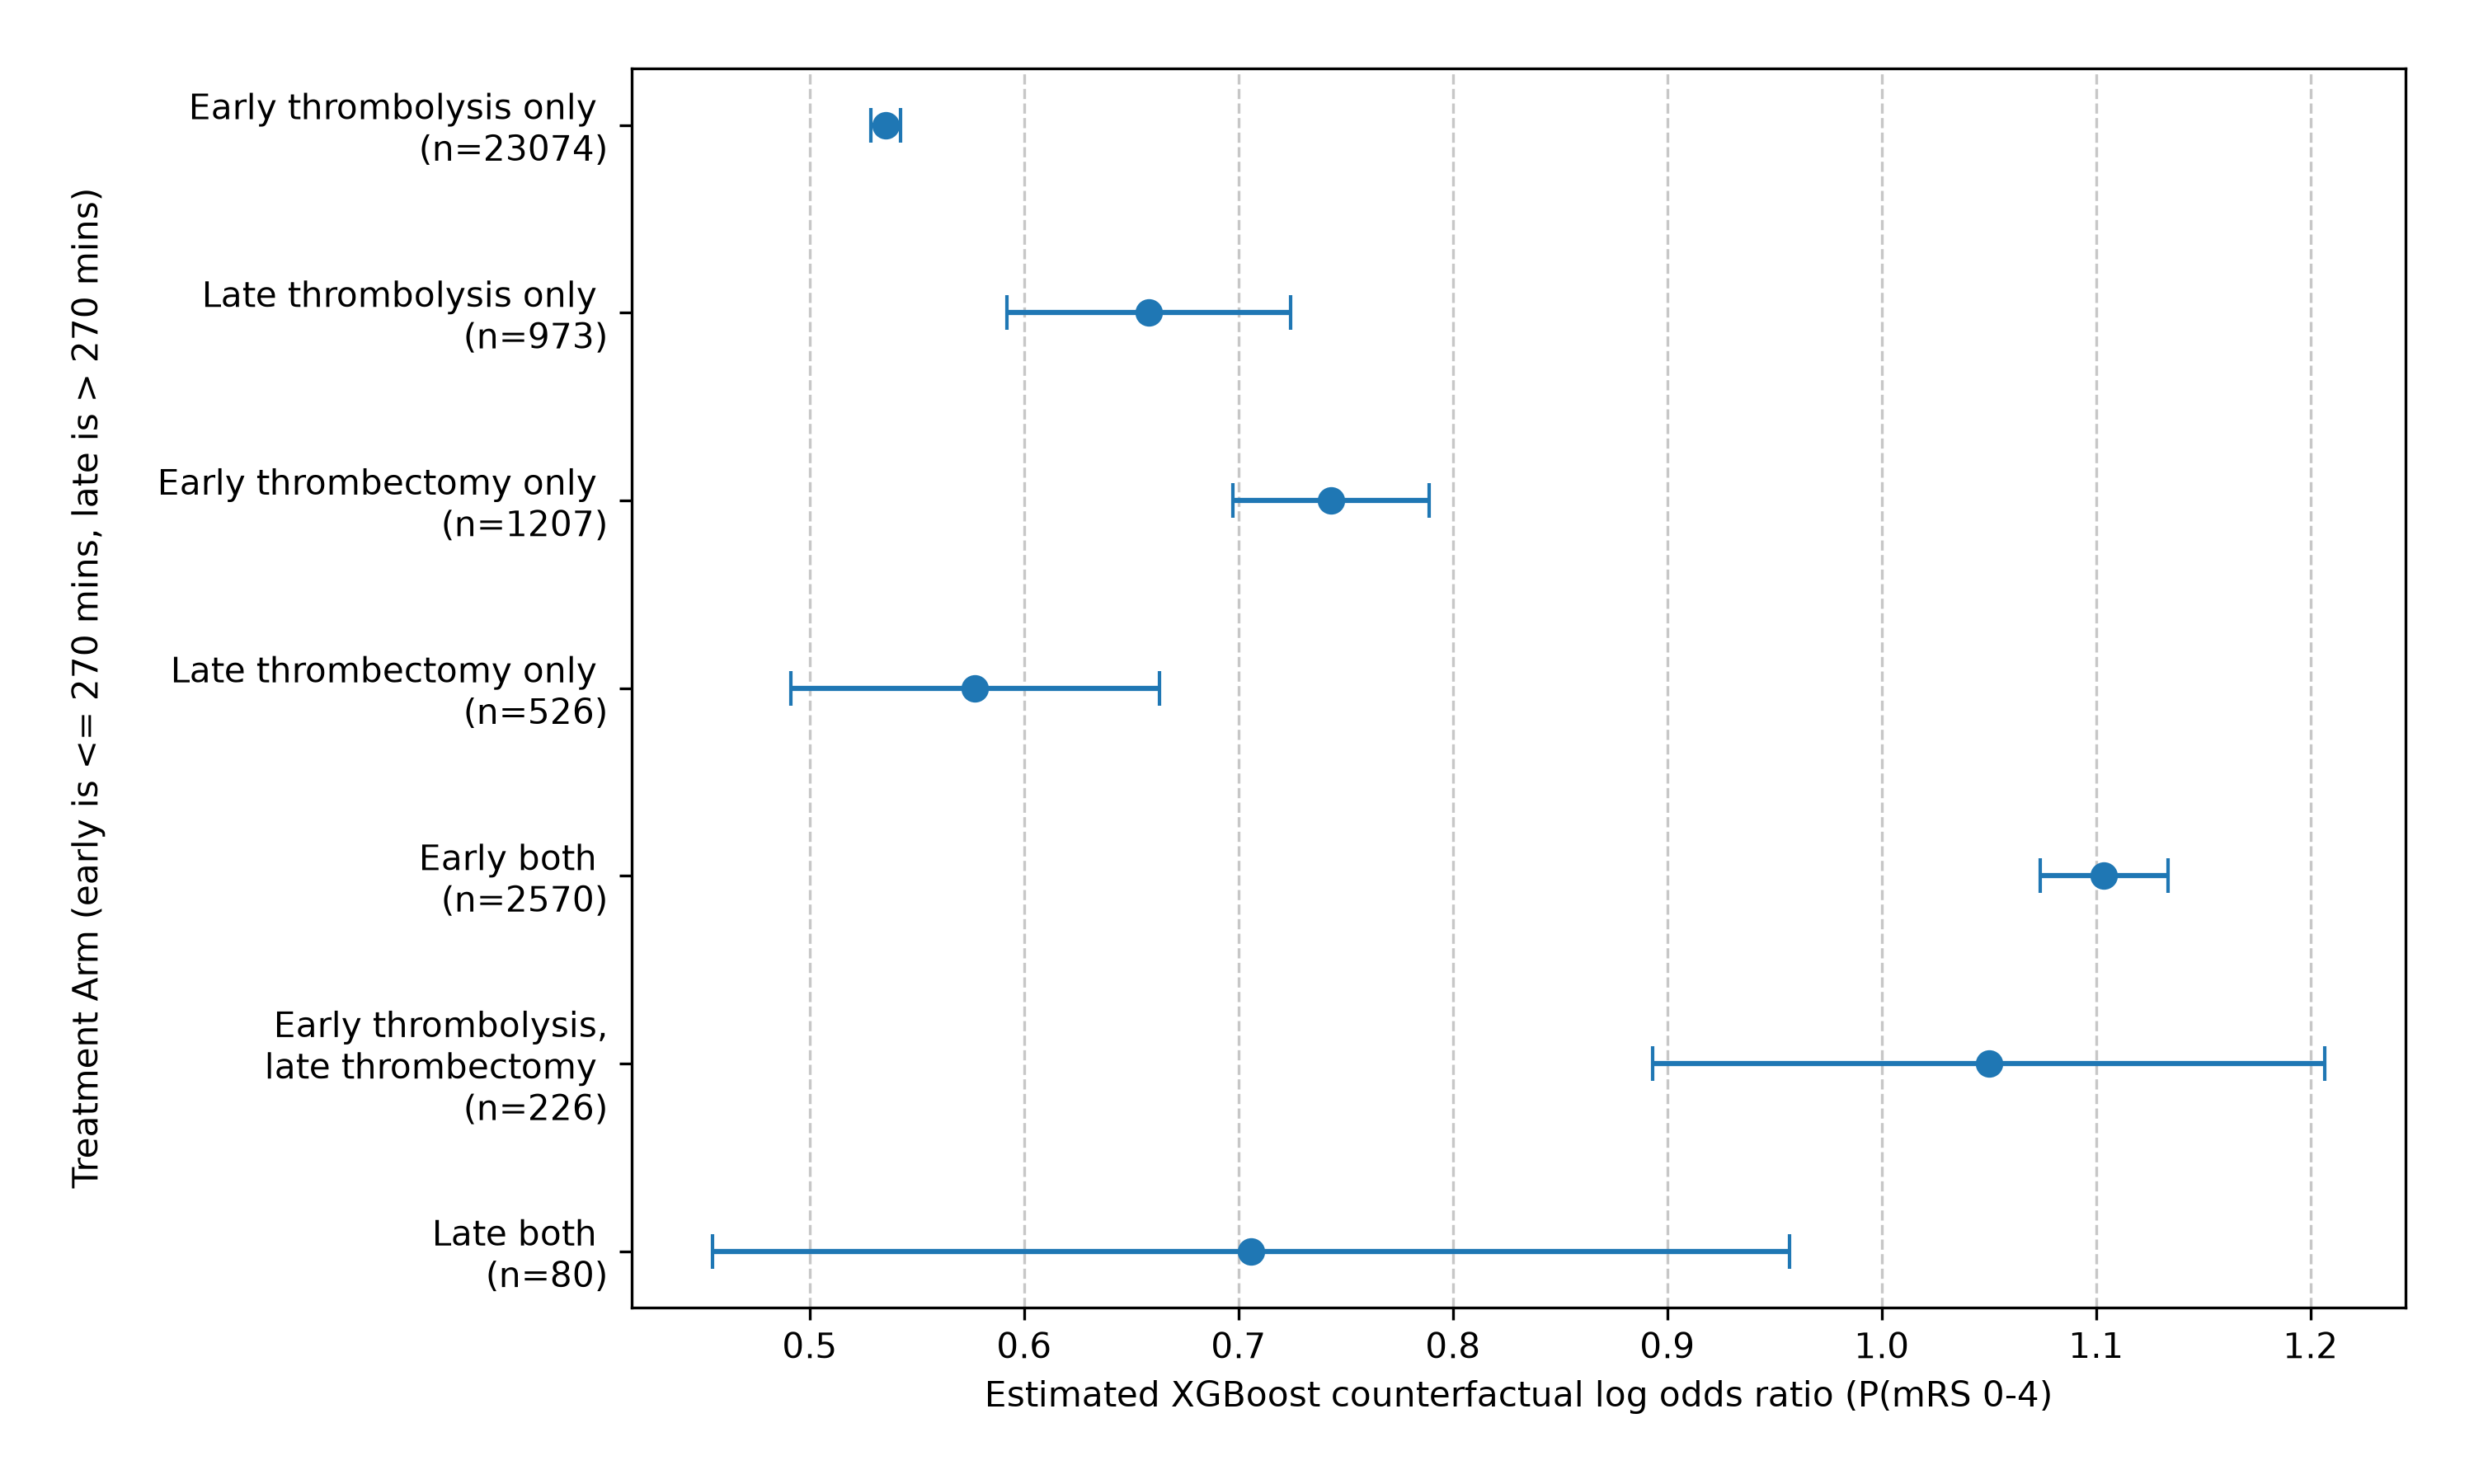
\includegraphics[width=\linewidth]{images/treatment_effects/xgboost_counterfactual_cate_log_odds_estimates_4}
        %\caption{}
        \label{fig:centre-right}
    \end{subfigure}

    \vspace{0.5cm} % Optional vertical space between rows

    % Bottom image
    \begin{subfigure}{0.48\textwidth}
        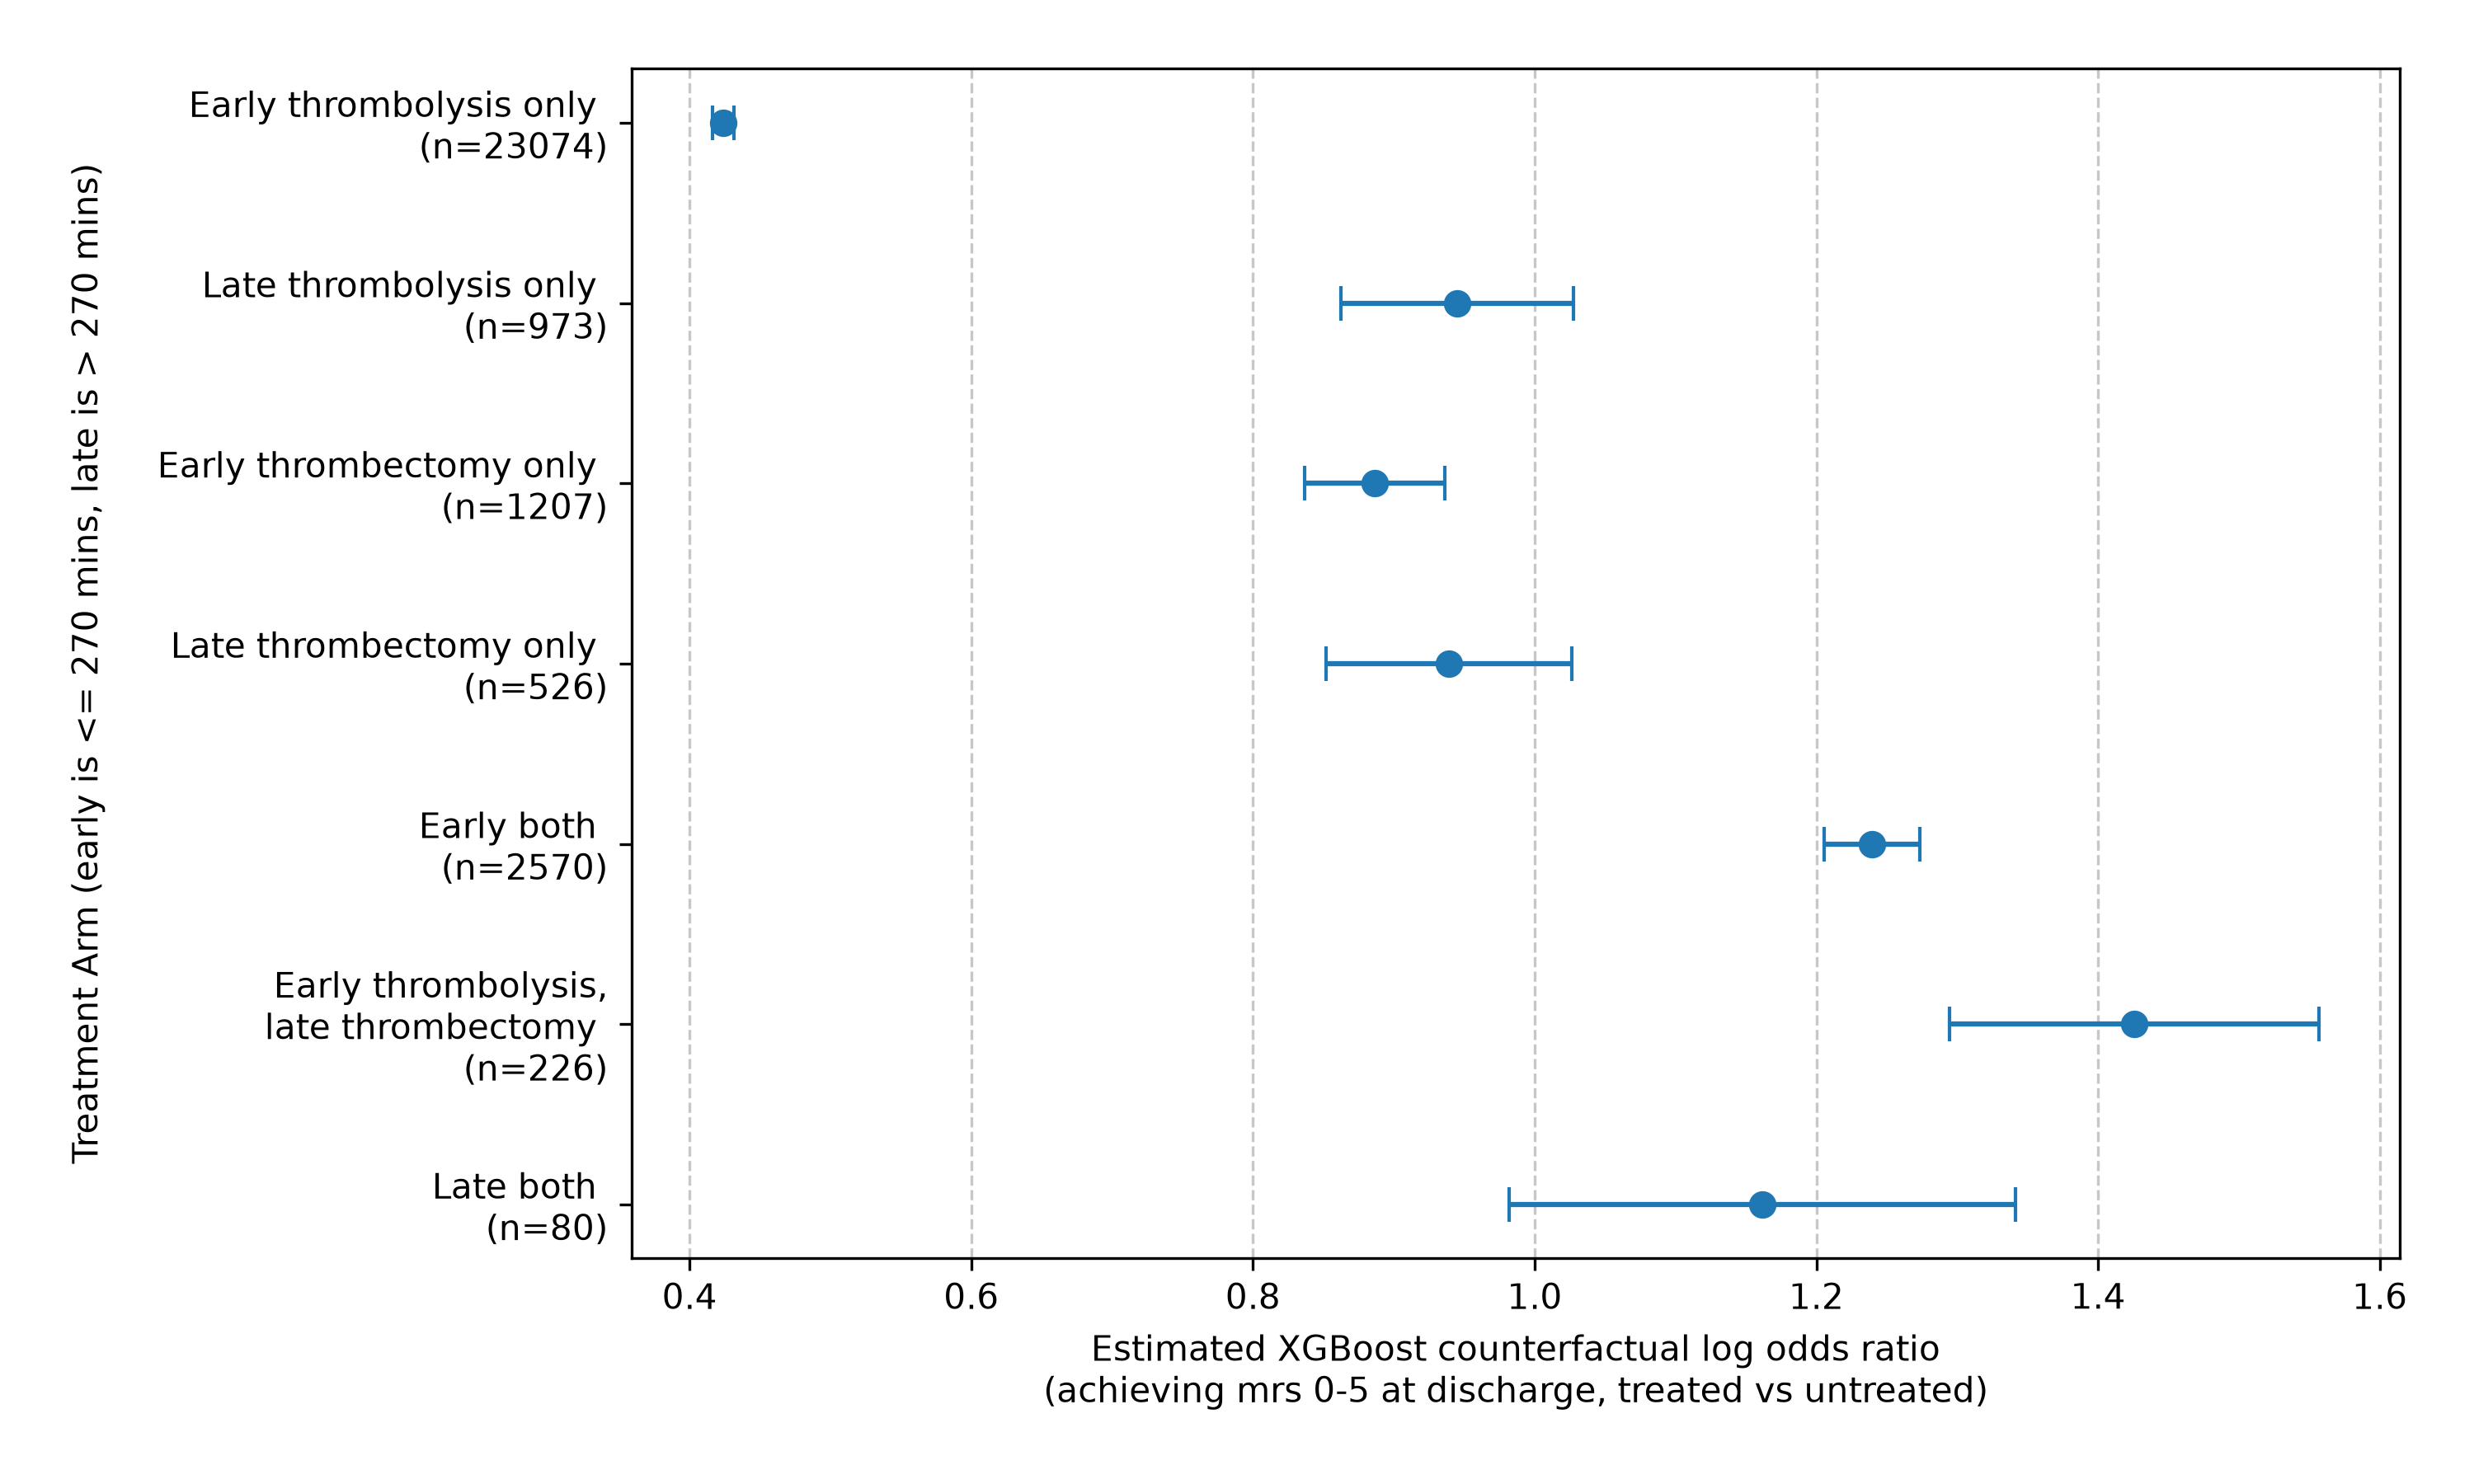
\includegraphics[width=\linewidth]{images/treatment_effects/xgboost_counterfactual_cate_log_odds_estimates_5}
        %\caption{}
        \label{fig:centre-right}
    \end{subfigure}
    
    \caption{Estimated counterfactual treatment benefit across reperfusion-treatment timing strategies, derived from the XGBoost S-learner model. Each panel shows results for discharge at or below each modified Rankin Scale (mRS) level. Points represent the mean estimated individual treatment effect for each treatment-timing group, expressed as the counterfactual log odds ratio for the specified outcome relative to no reperfusion treatment; horizontal error bars show 95\% confidence intervals. Treatment groups are defined by receipt of intravenous thrombolysis and/or mechanical thrombectomy, with early treatment defined as onset-to-treatment time $<$270 minutes and late treatment as $\geq$270 minutes. Sample sizes are shown alongside group labels. Values above zero indicate a model-predicted increase in the odds of achieving the corresponding mRS outcome under the observed treatment strategy compared with no treatment.}
    \label{fig:s_learner_benefit}
\end{figure}



%%%%%%%%%%%%%%%%%%%%%%%%%%%%%%%%%%%%%%%%%%

Figure \ref{fig:s_learner_heatmap_log odds} shows a heatmap of the estimated benefit of thrombolysis and thrombectomy by use and speed in achieving each mRS threshold. This model used actual onset-to-treatment times for each of thrombolysis and thrombectomy. Resulting benefit, estimated using counterfactual modelling, was binned by time (in hours) of treatment after stroke onset.

\begin{figure}[htbp]
    \centering
    
    % Top left
    \begin{subfigure}{0.48\textwidth}
        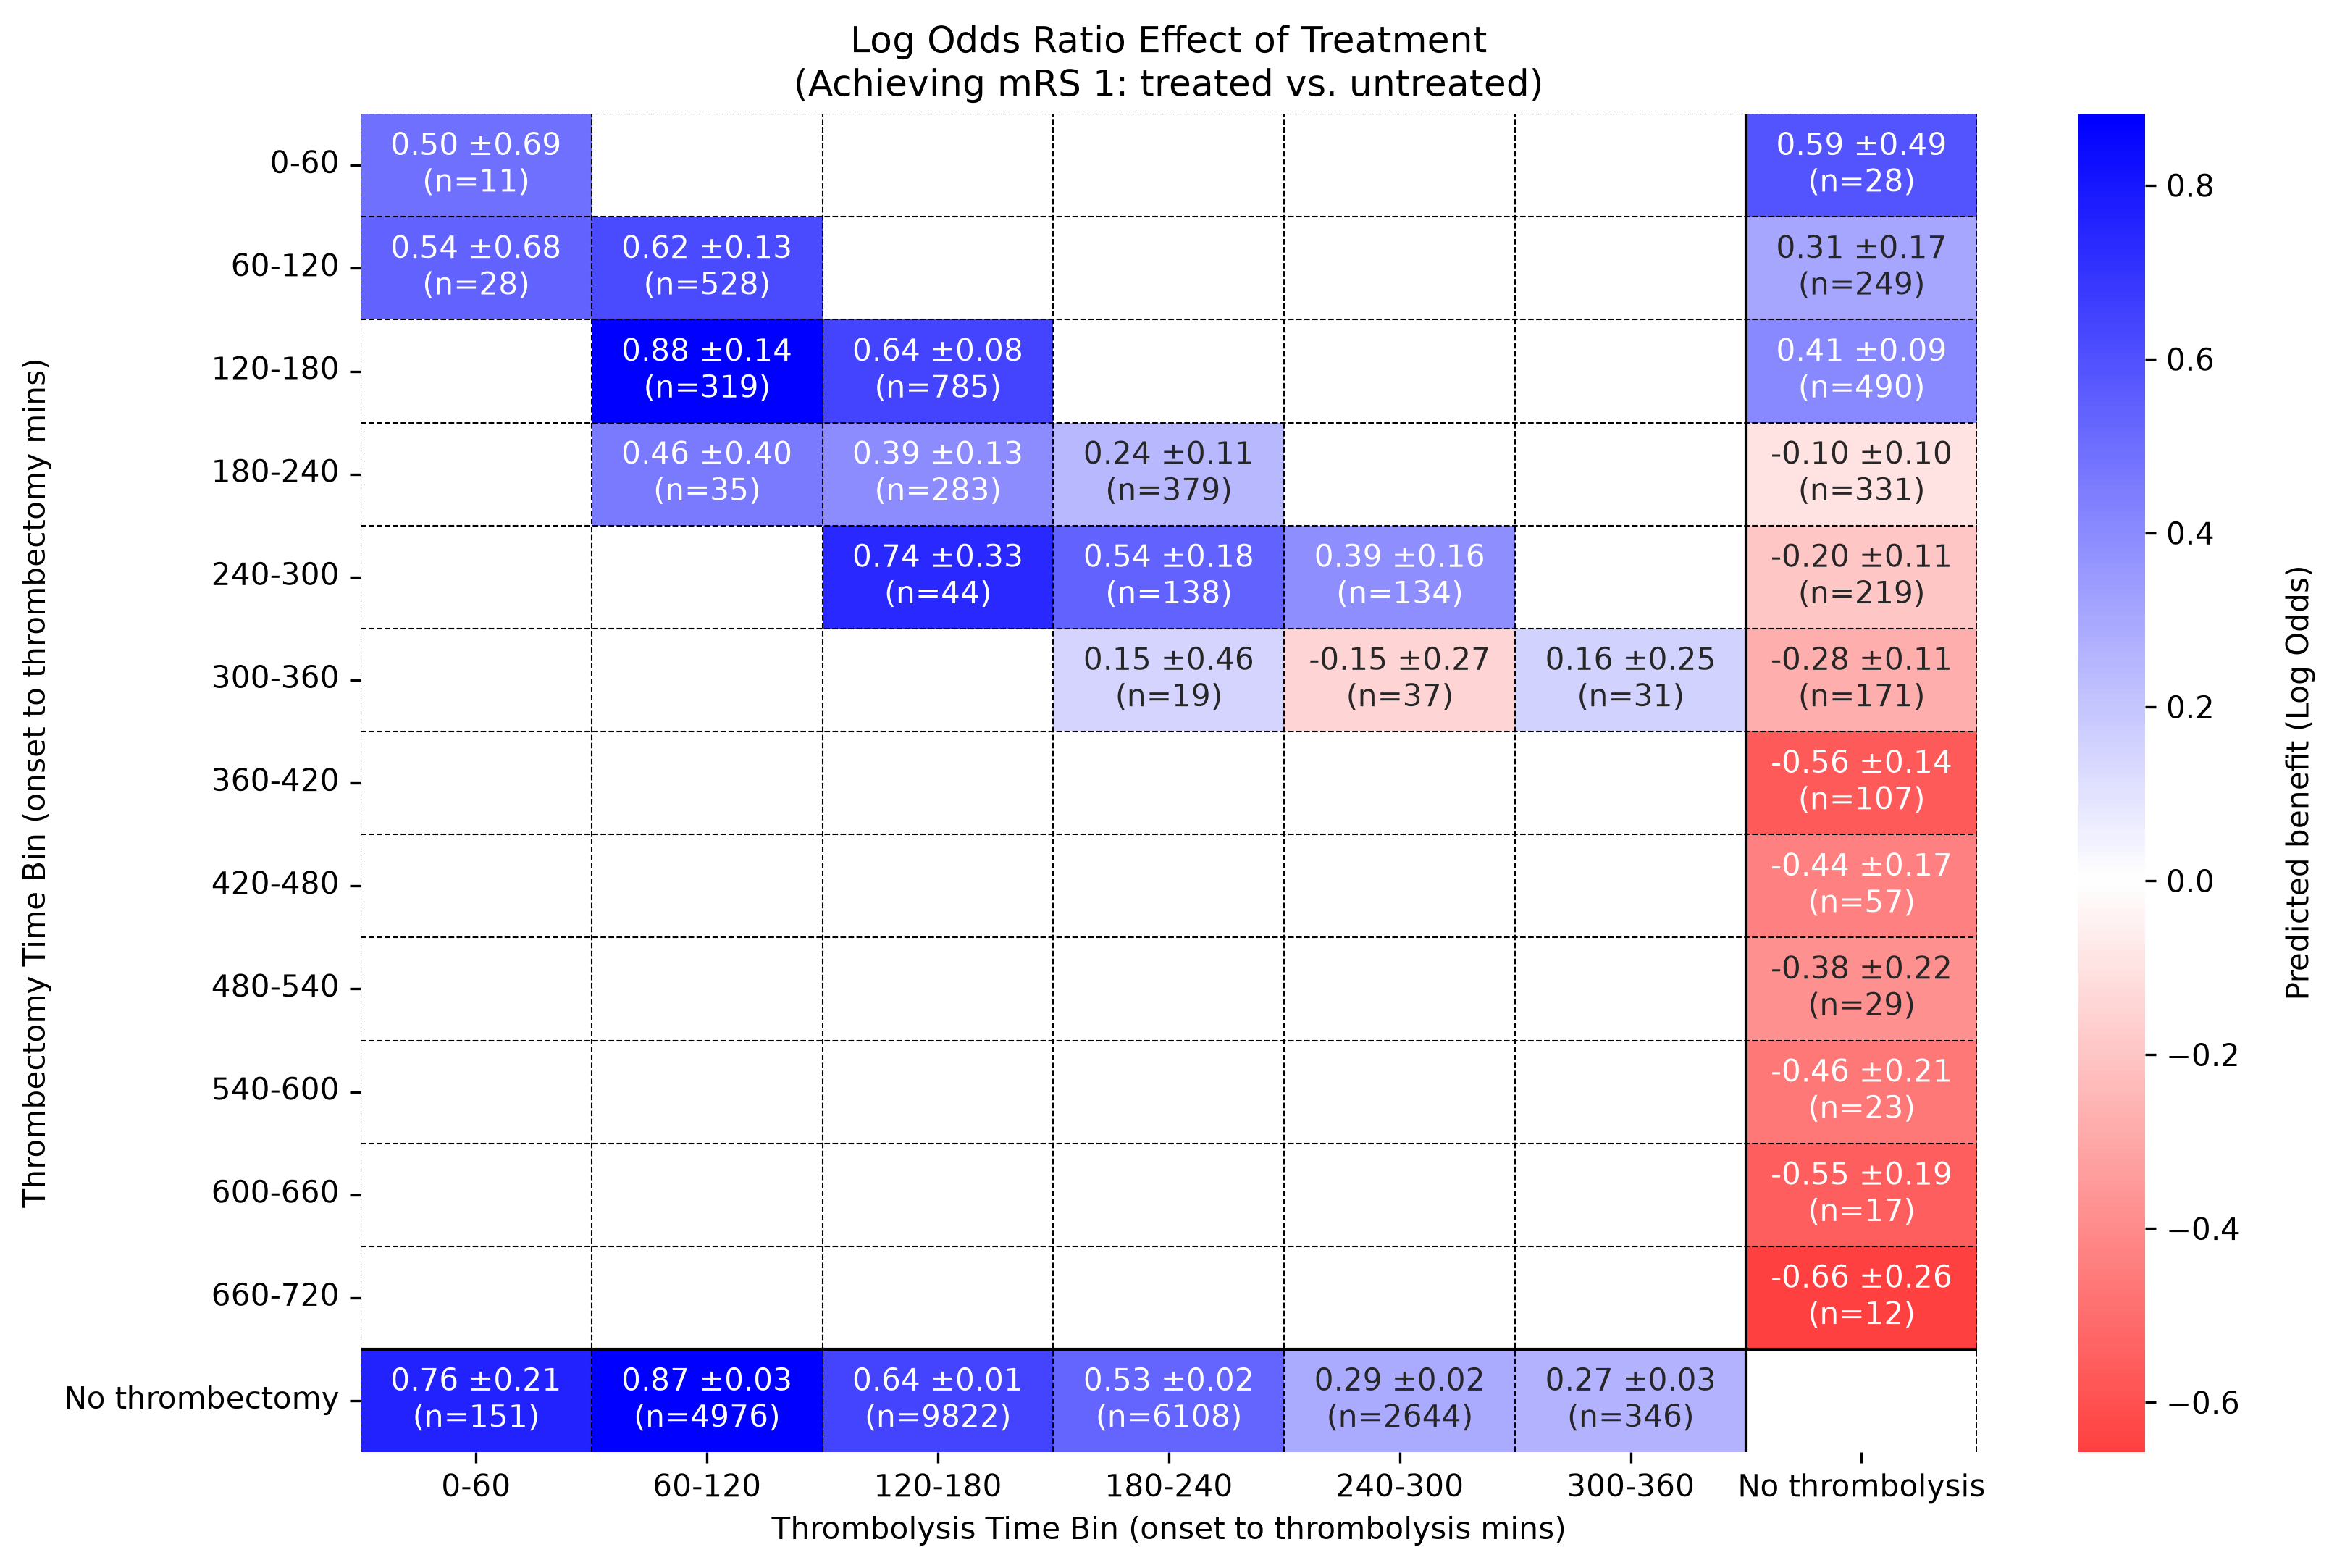
\includegraphics[width=\linewidth]{images/treatment_effects/thrombolysis_thrombectomy_heatmap_mrs_1.png}
        %\caption{}
        \label{fig:top-left}
    \end{subfigure}
    \hfill % Adds flexible horizontal spacing
    % top right image 
    \begin{subfigure}{0.48\textwidth}
        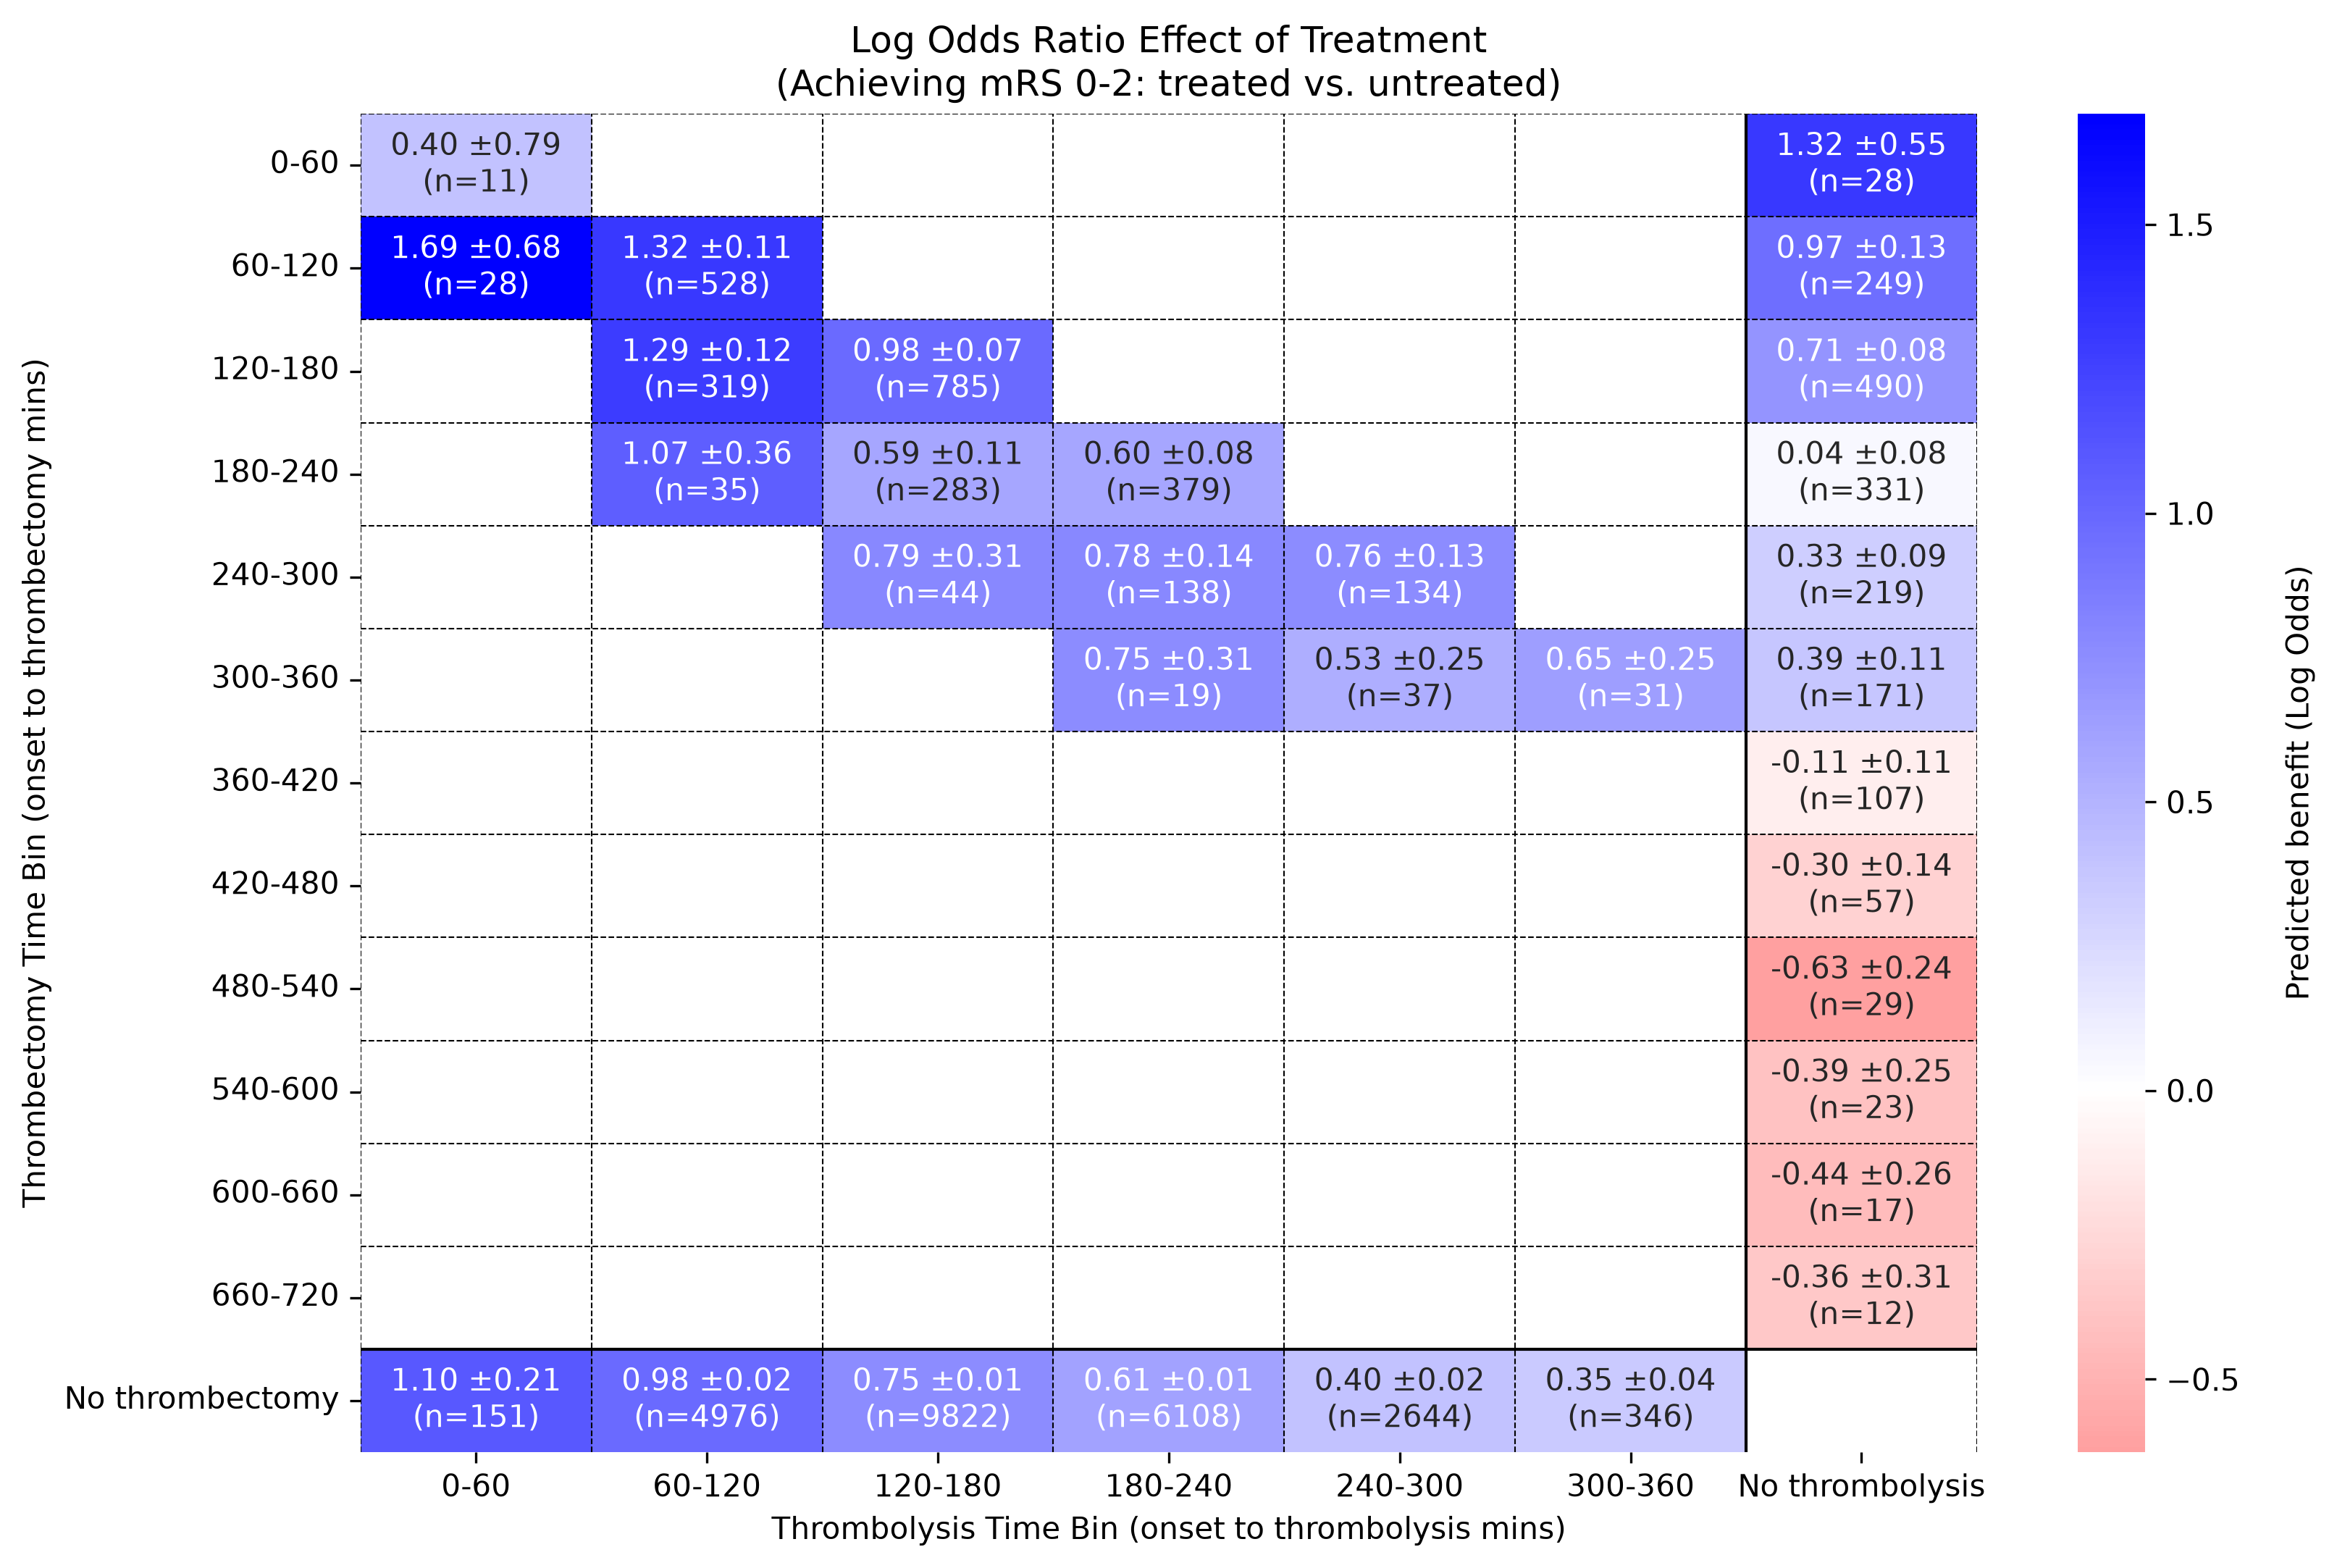
\includegraphics[width=\linewidth]{images/treatment_effects/thrombolysis_thrombectomy_heatmap_mrs_2.png}
        %\caption{}
        \label{fig:bottom-left}
    \end{subfigure}

    \vspace{0.5cm} % Optional vertical space between rows

    % Center left image
    \begin{subfigure}{0.48\textwidth}
        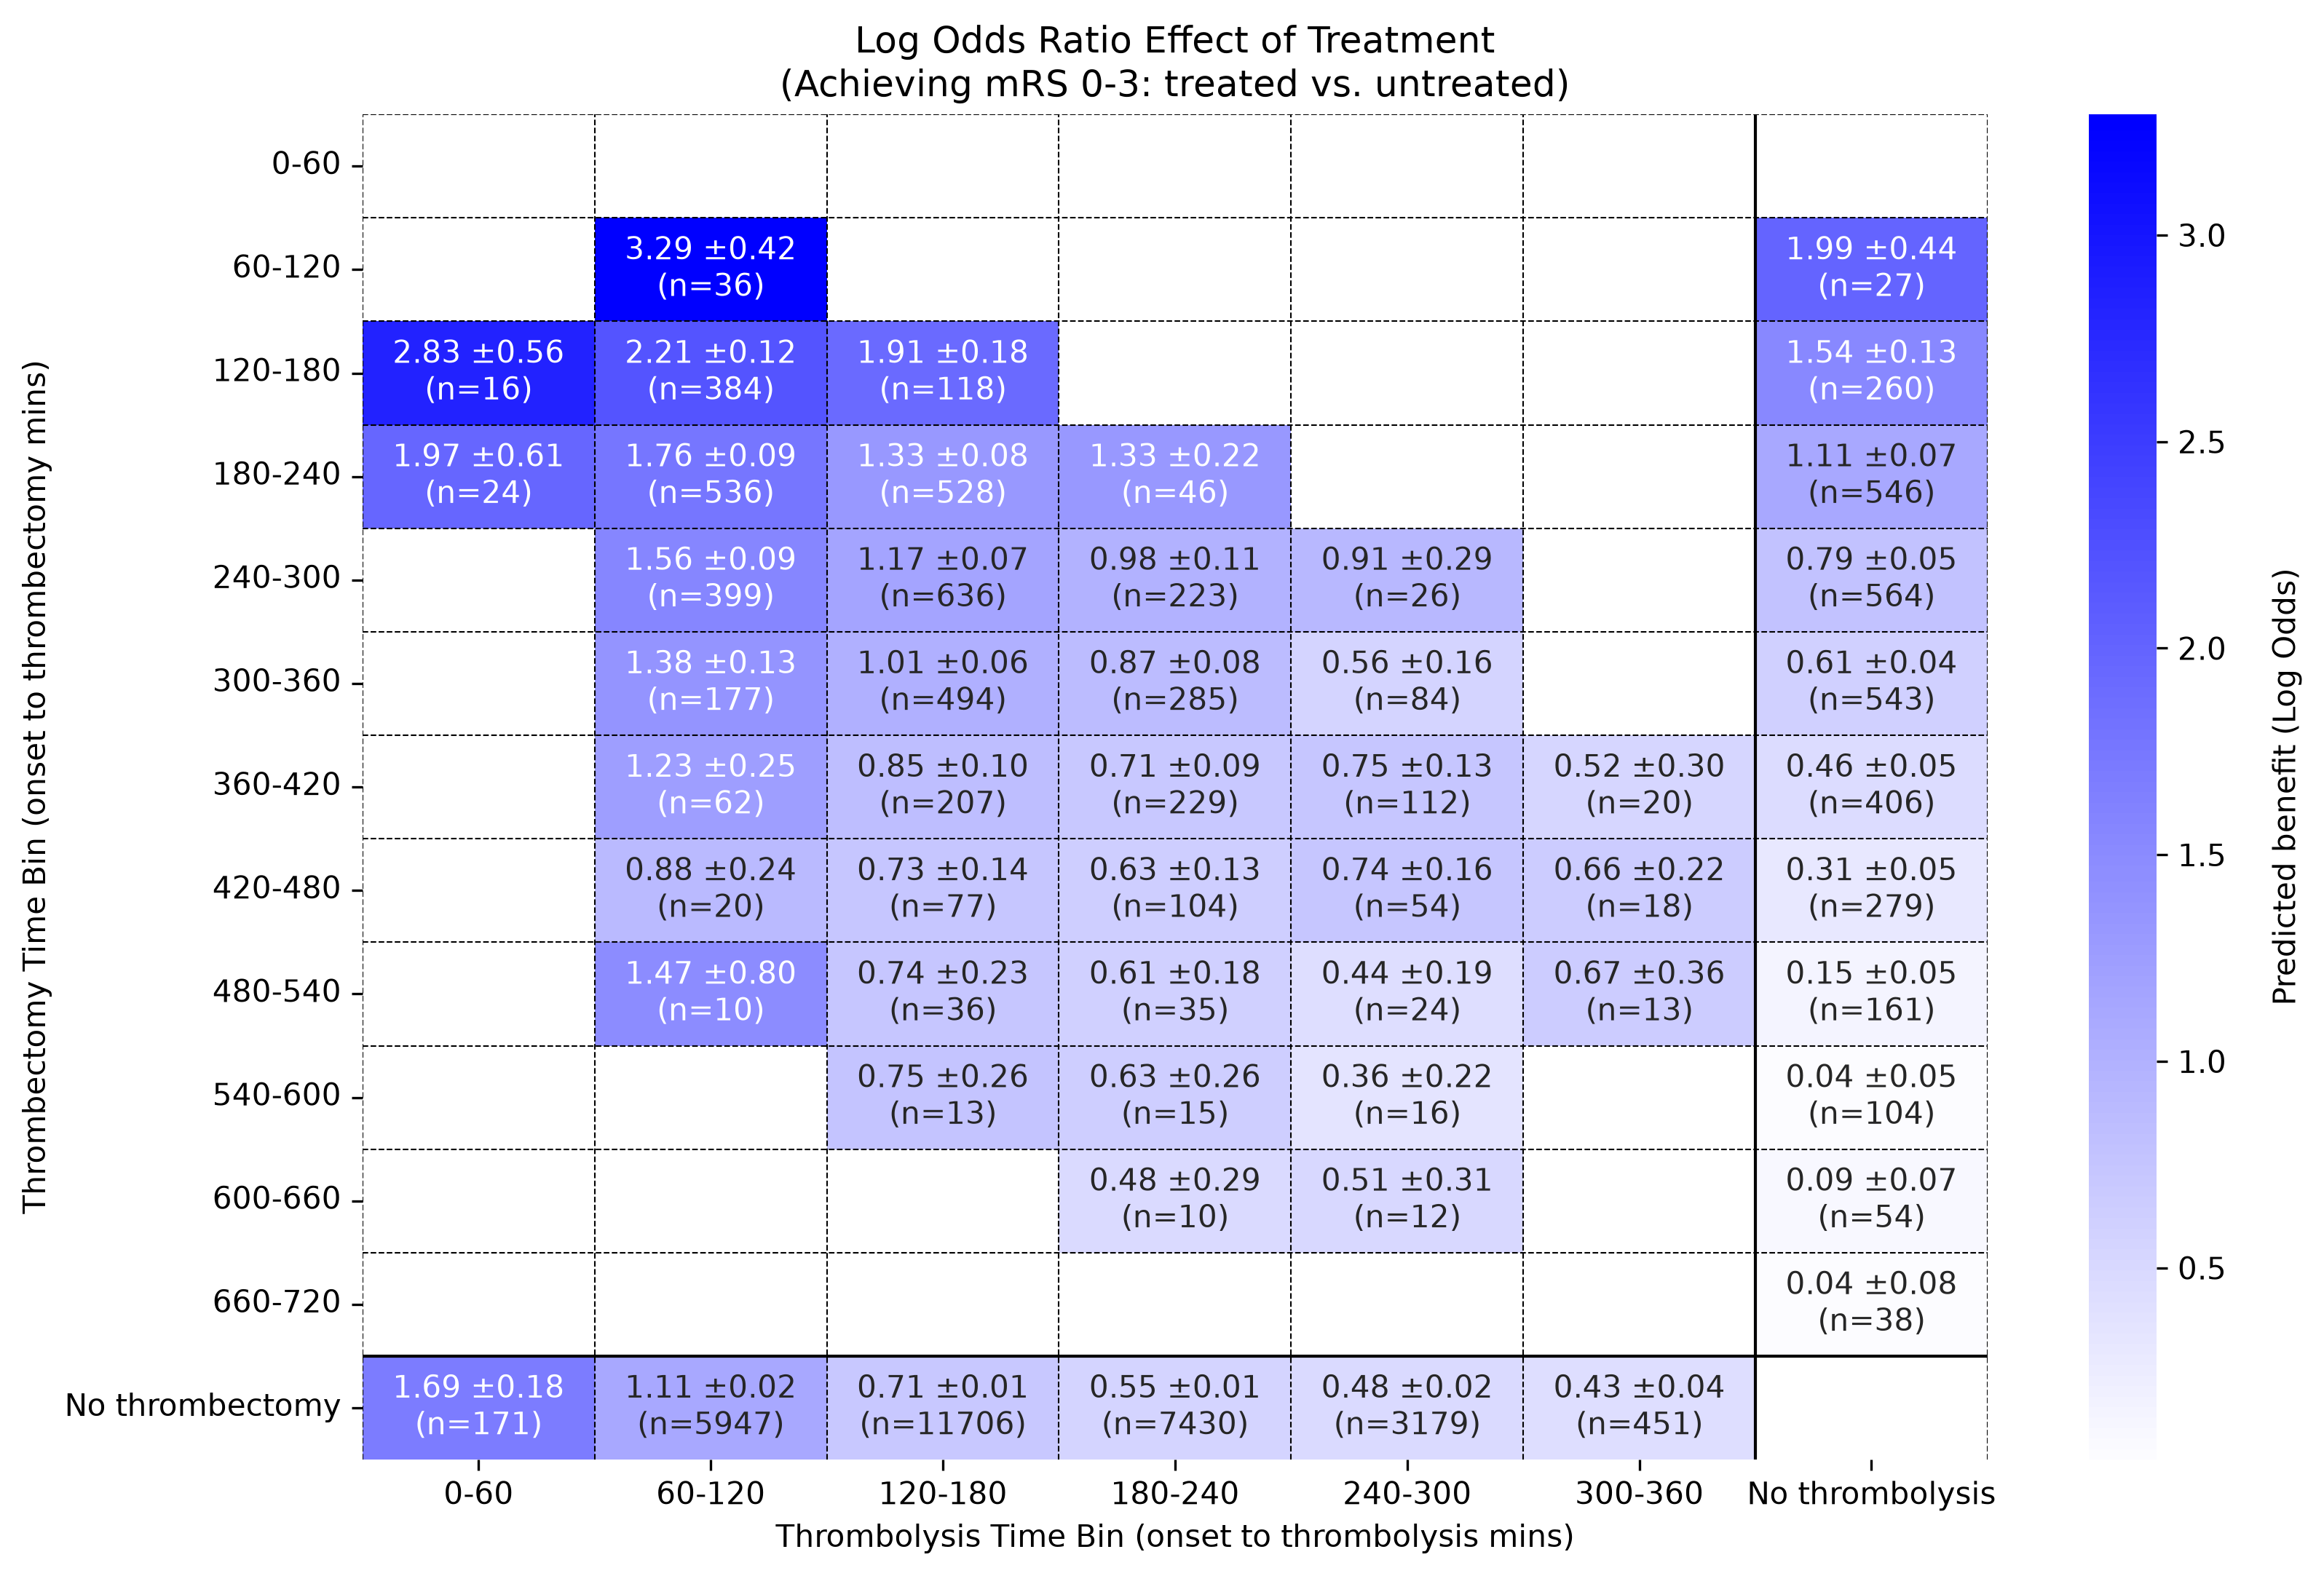
\includegraphics[width=\linewidth]{images/treatment_effects/thrombolysis_thrombectomy_heatmap_mrs_3.png}
        %\caption{}
        \label{fig:centre-left}
    \end{subfigure}
    \hfill % Adds flexible horizontal spacing
    % Centre right image 
    \begin{subfigure}{0.48\textwidth}
        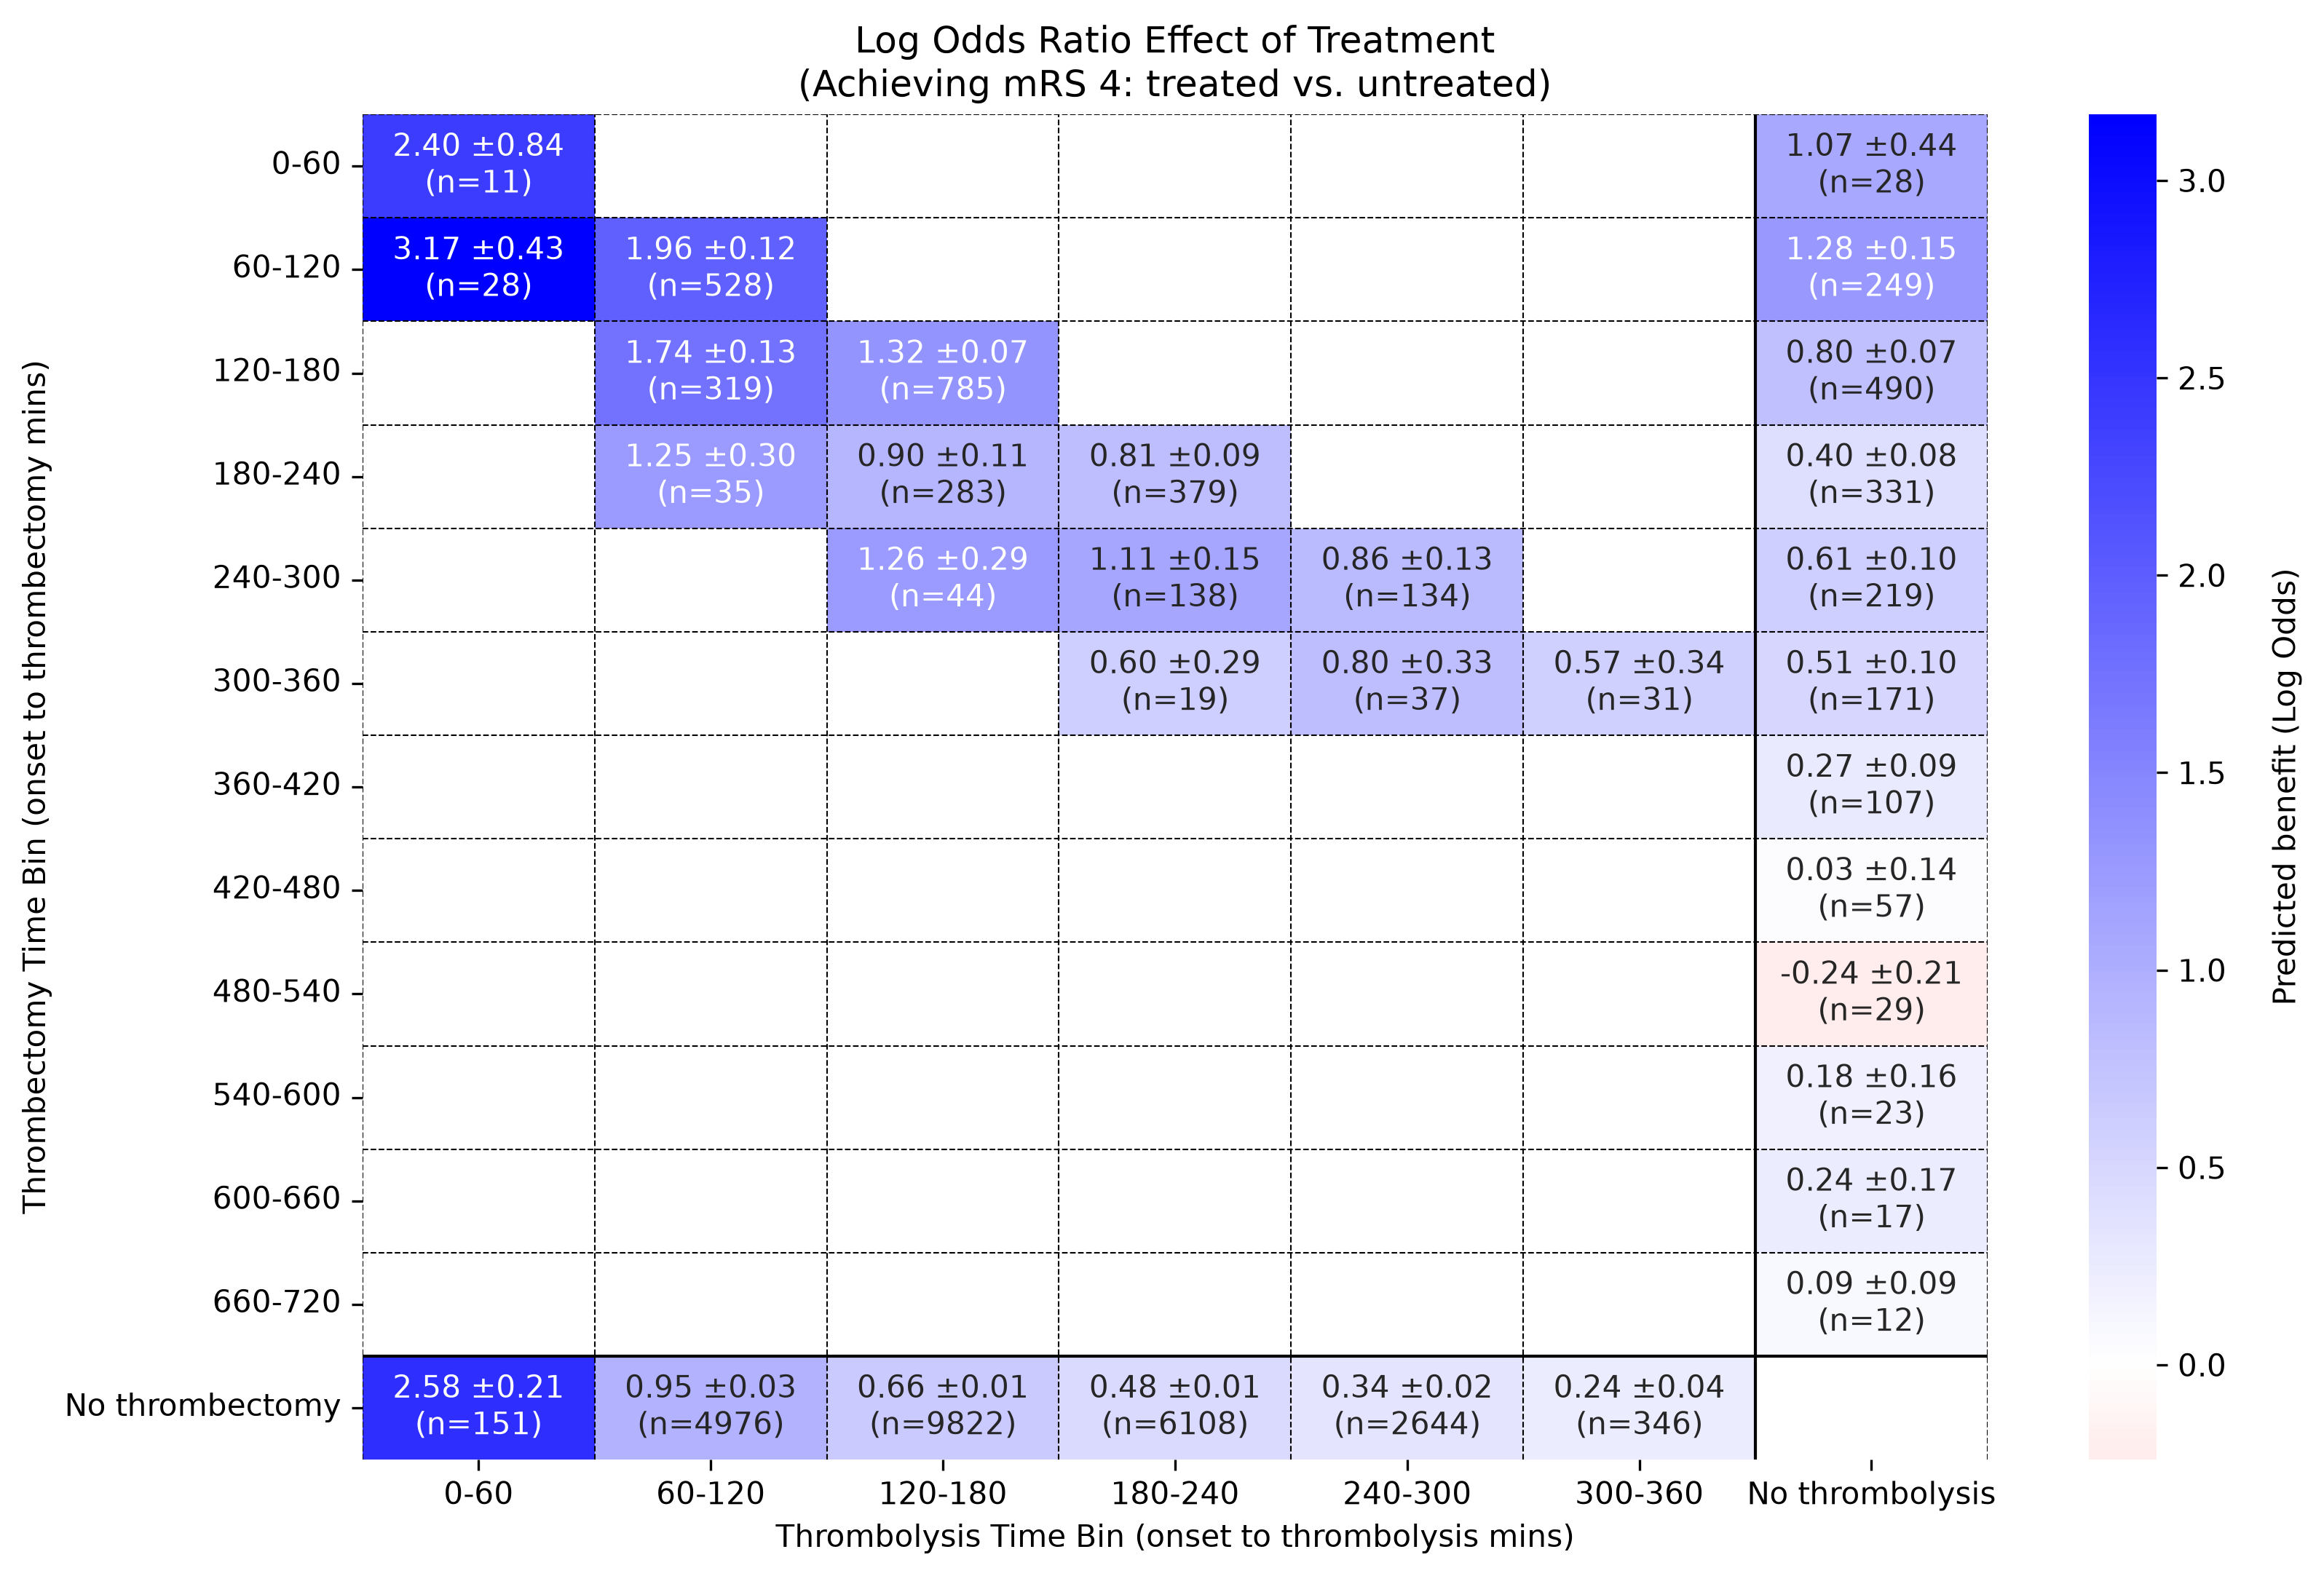
\includegraphics[width=\linewidth]{images/treatment_effects/thrombolysis_thrombectomy_heatmap_mrs_4.png}
        %\caption{}
        \label{fig:centre-right}
    \end{subfigure}

    \vspace{0.5cm} % Optional vertical space between rows

    % Bottom image
    \begin{subfigure}{0.48\textwidth}
        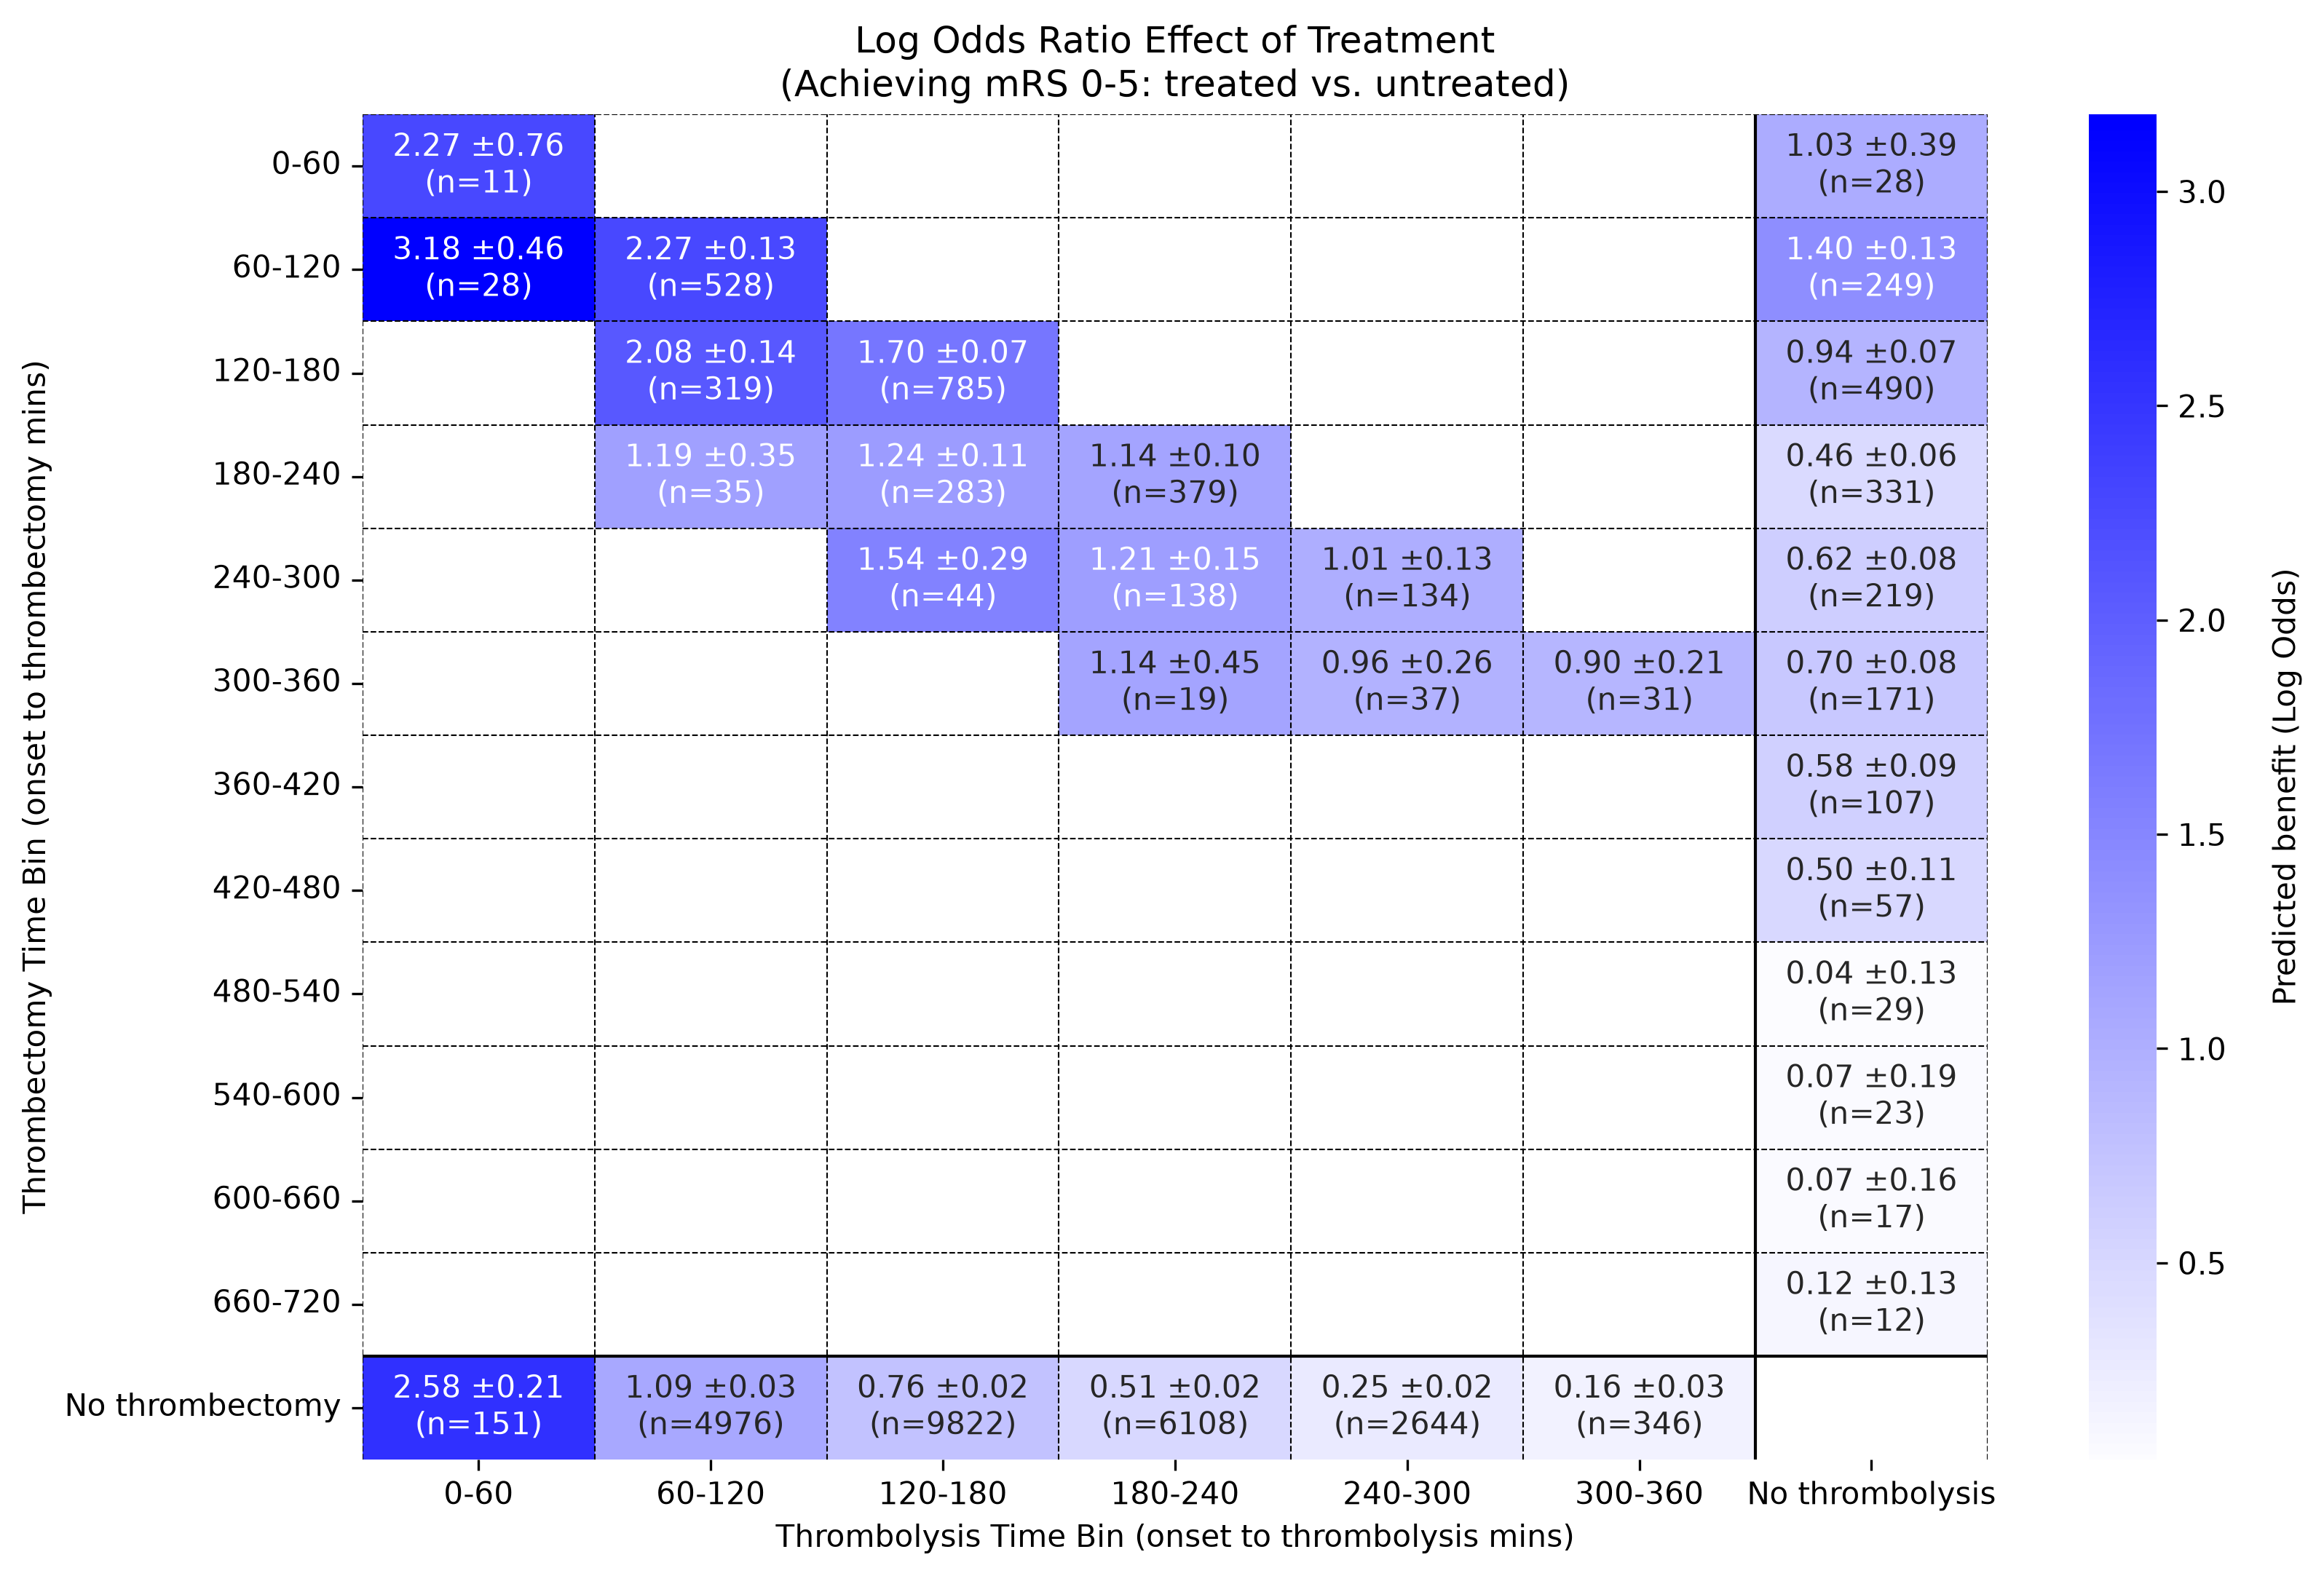
\includegraphics[width=\linewidth]{images/treatment_effects/thrombolysis_thrombectomy_heatmap_mrs_5}
        %\caption{}
        \label{fig:centre-right}
    \end{subfigure}
    
    \caption{Predicted treatment benefit by thrombolysis and thrombectomy timing from the S-learner XGBoost model. Each panel shows a heatmap of the model-estimated effect of treatment on the log-odds of being discharged at each modified Rankin Scale (mRS) level, comparing treated with untreated patients across combinations of onset-to-thrombolysis and onset-to-thrombectomy time intervals. Each cell reports the mean predicted treatment benefit ± standard deviation, with the number of patients in parentheses. Blue shading denotes a positive predicted effect of treatment (increased log-odds of achieving each mRS level), whereas red shading denotes a negative predicted effect. The final row and column represent patients receiving thrombectomy without thrombolysis and thrombolysis without thrombectomy, respectively; blank cells indicate treatment-timing combinations with fewer than 10 observations in the data}
    \label{fig:s_learner_heatmap_log odds}
\end{figure}



%%%%%%%%%%%%%%%%%%%%%%%%%%%%%%%%%%%%%%%%%%

Figure \ref{fig:s_learner_time_thrombolysis} shows a scatter plot, with regression line, of of the estimated benefit of thrombolysis (log odds ratio, treated vs untreated), by time after onset, in achieving each mRS threshold. This model used actual onset-to-treatment times for thrombolysis, and is for patients receiving thrombolysis only.

\begin{figure}[htbp]
    \centering
    
    % Top left
    \begin{subfigure}{0.38\textwidth}
        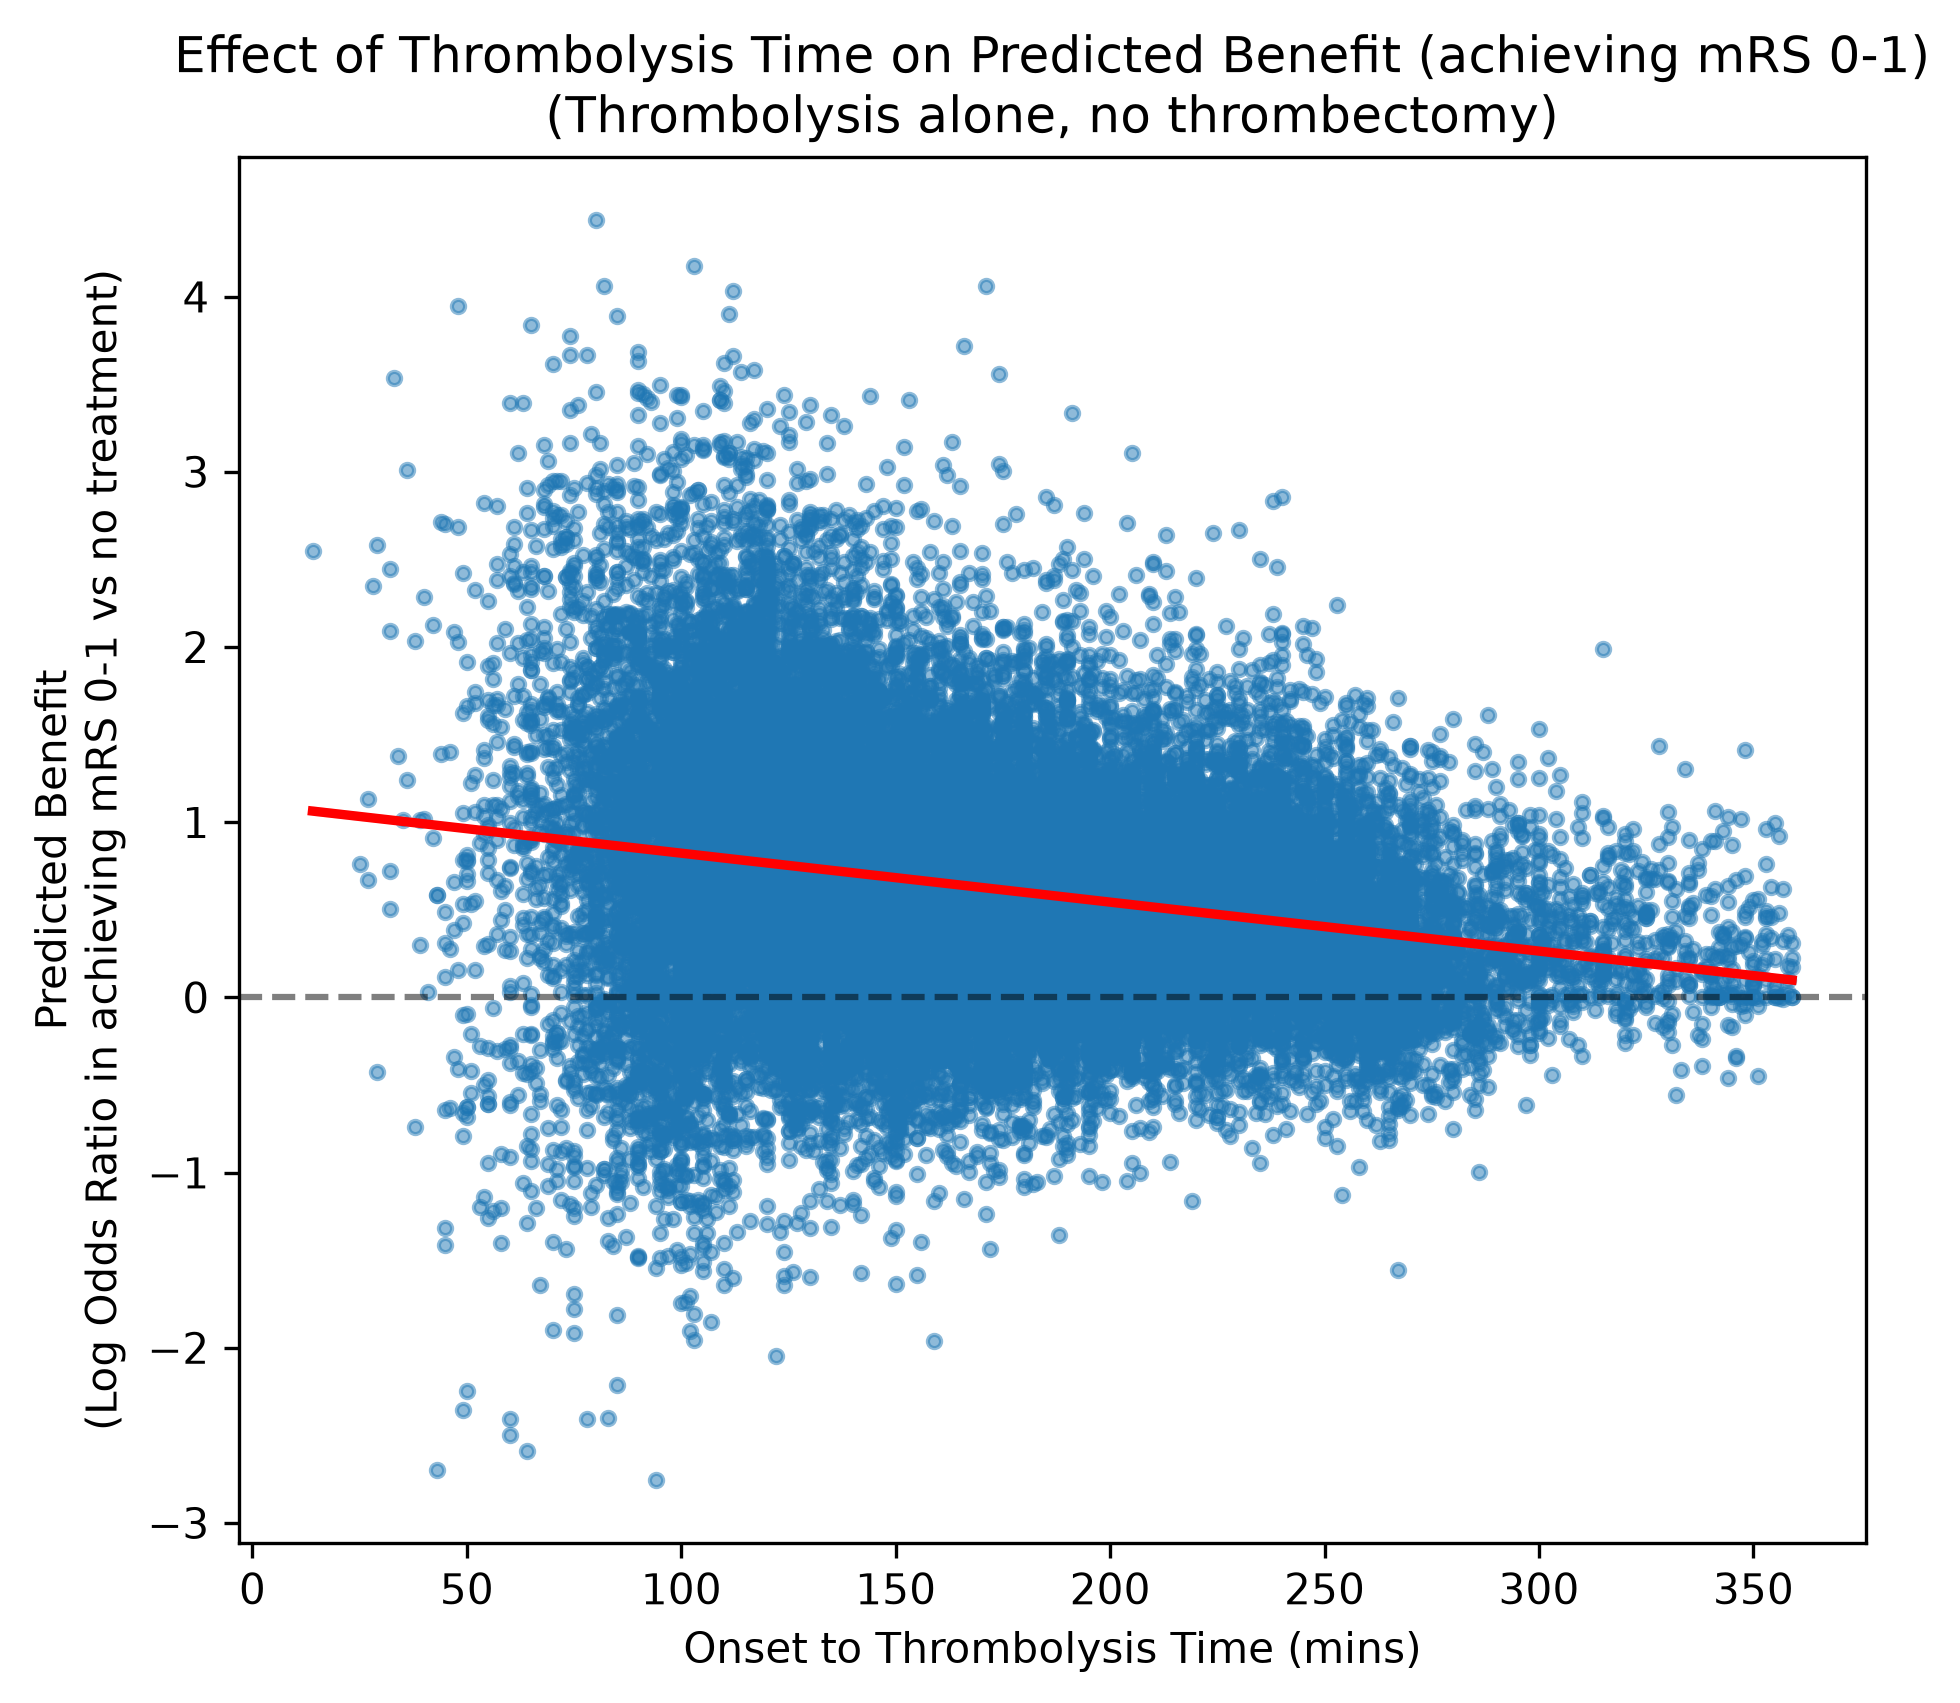
\includegraphics[width=\linewidth]{images/treatment_effects/thrombolysis_alone_time_effect_mrs_1.png}
        %\caption{}
        \label{fig:top-left}
    \end{subfigure}
    %\hfill % Adds flexible horizontal spacing
    % top right image 
    \begin{subfigure}{0.38\textwidth}
        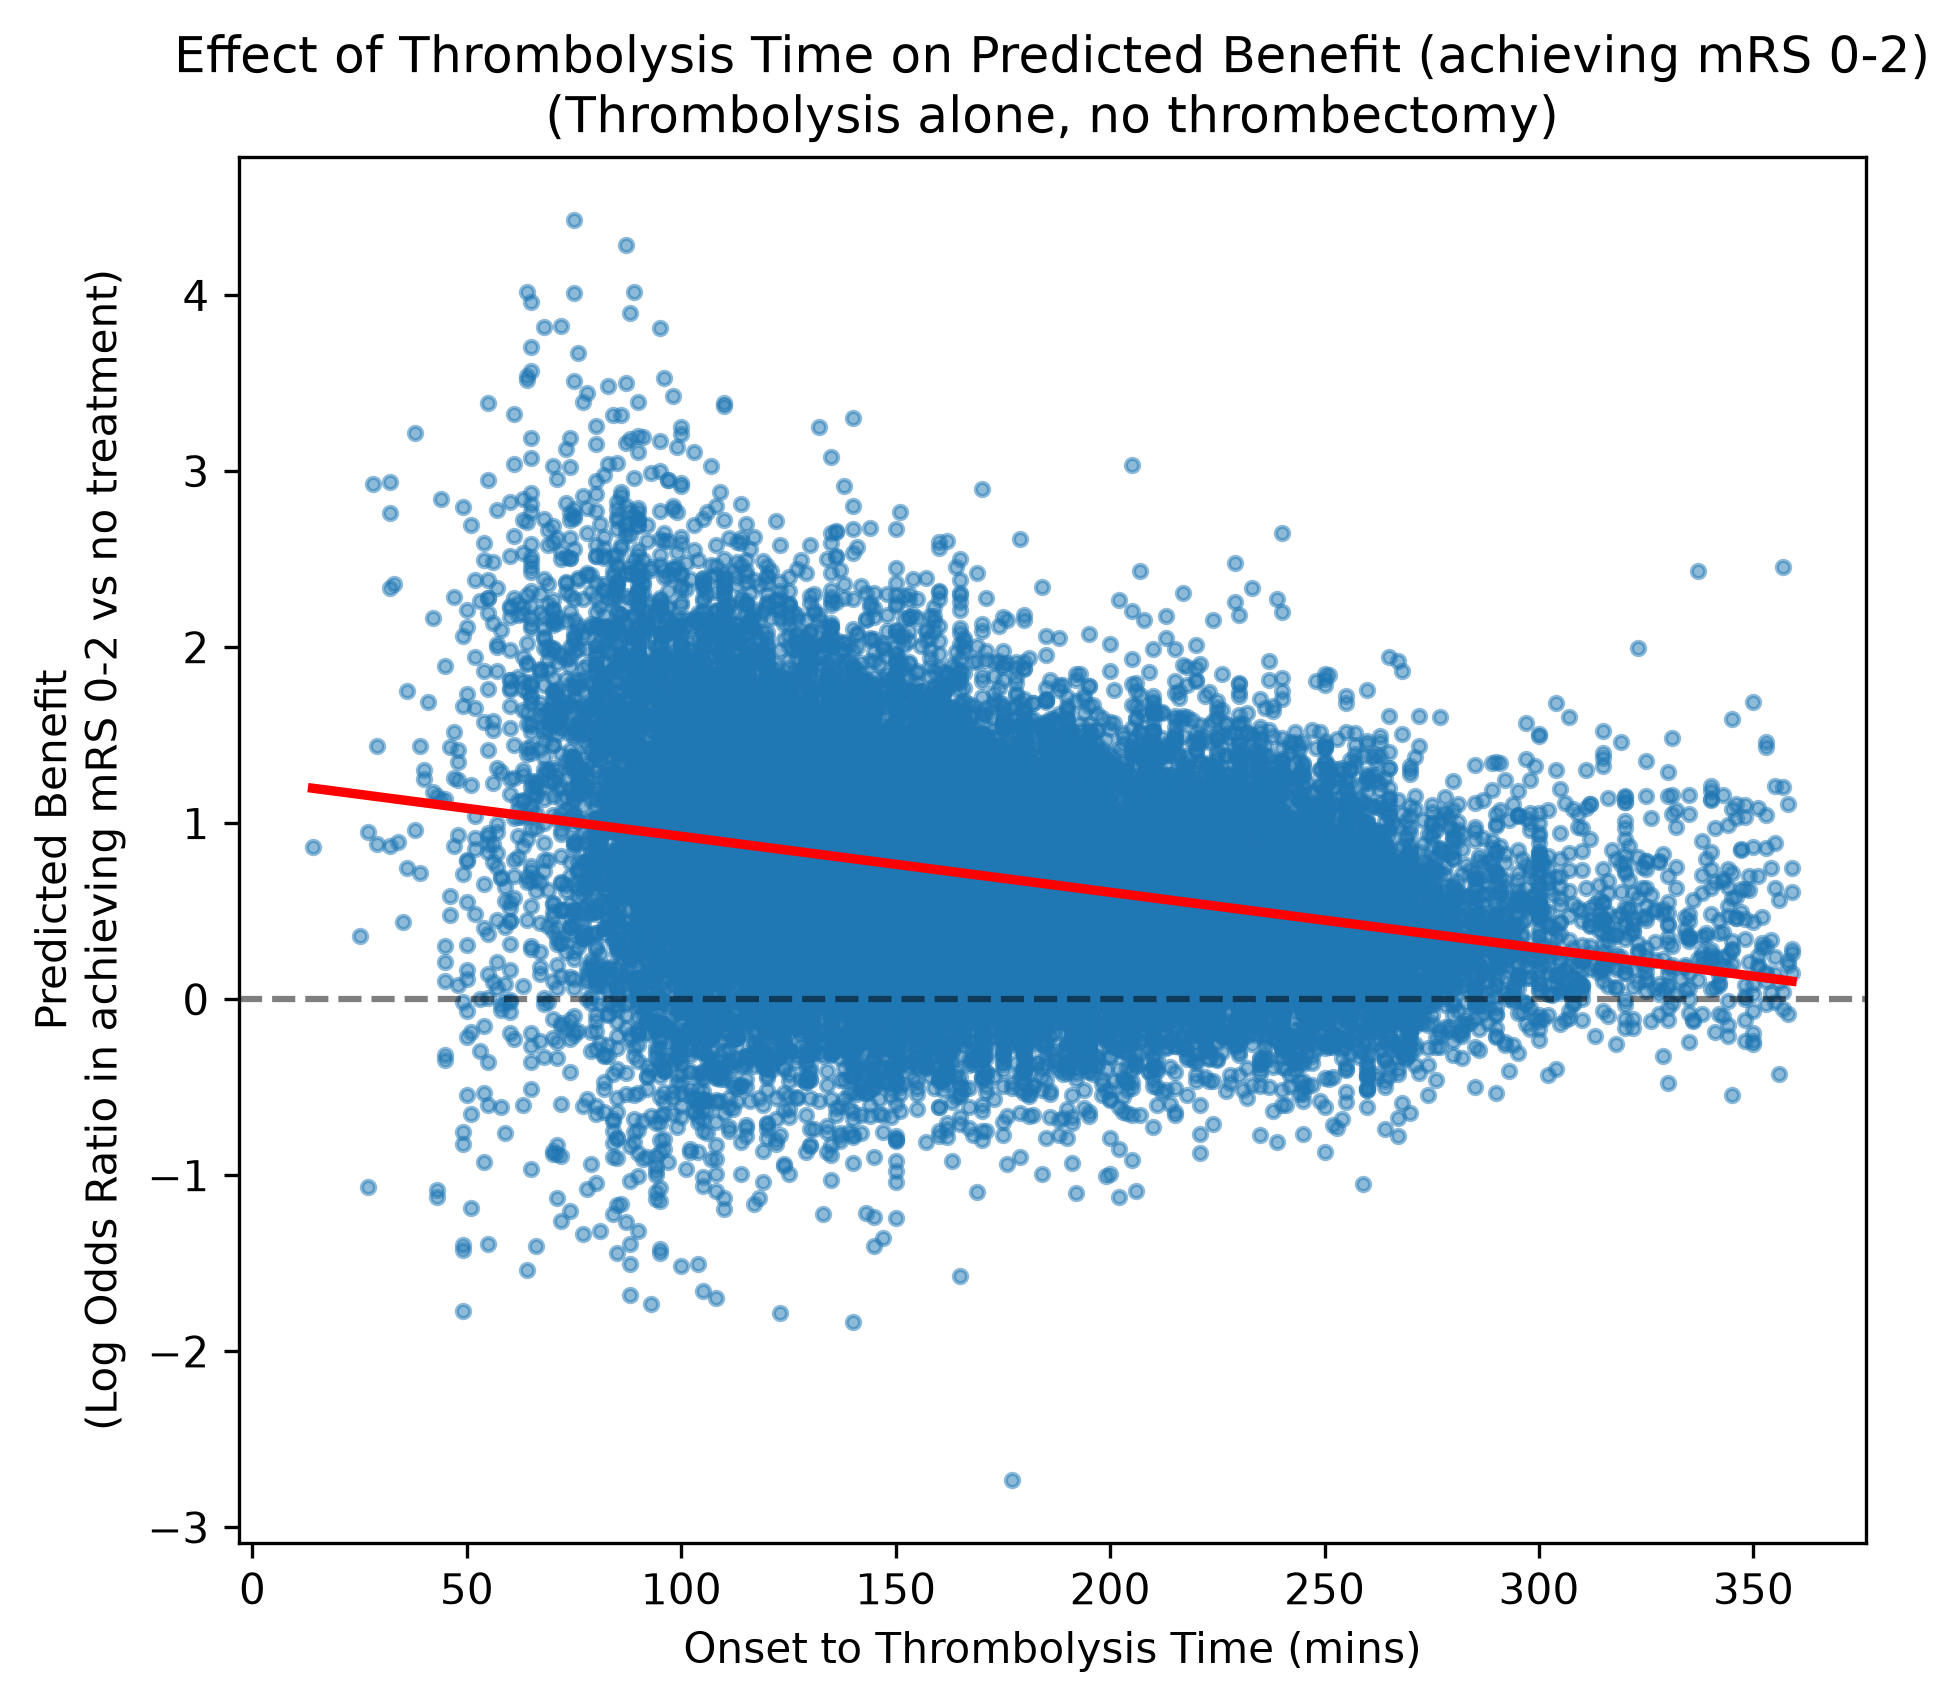
\includegraphics[width=\linewidth]{images/treatment_effects/thrombolysis_alone_time_effect_mrs_2.png}
        %\caption{}
        \label{fig:bottom-left}
    \end{subfigure}

    \vspace{0.2cm} % Optional vertical space between rows

    % Center left image
    \begin{subfigure}{0.38\textwidth}
        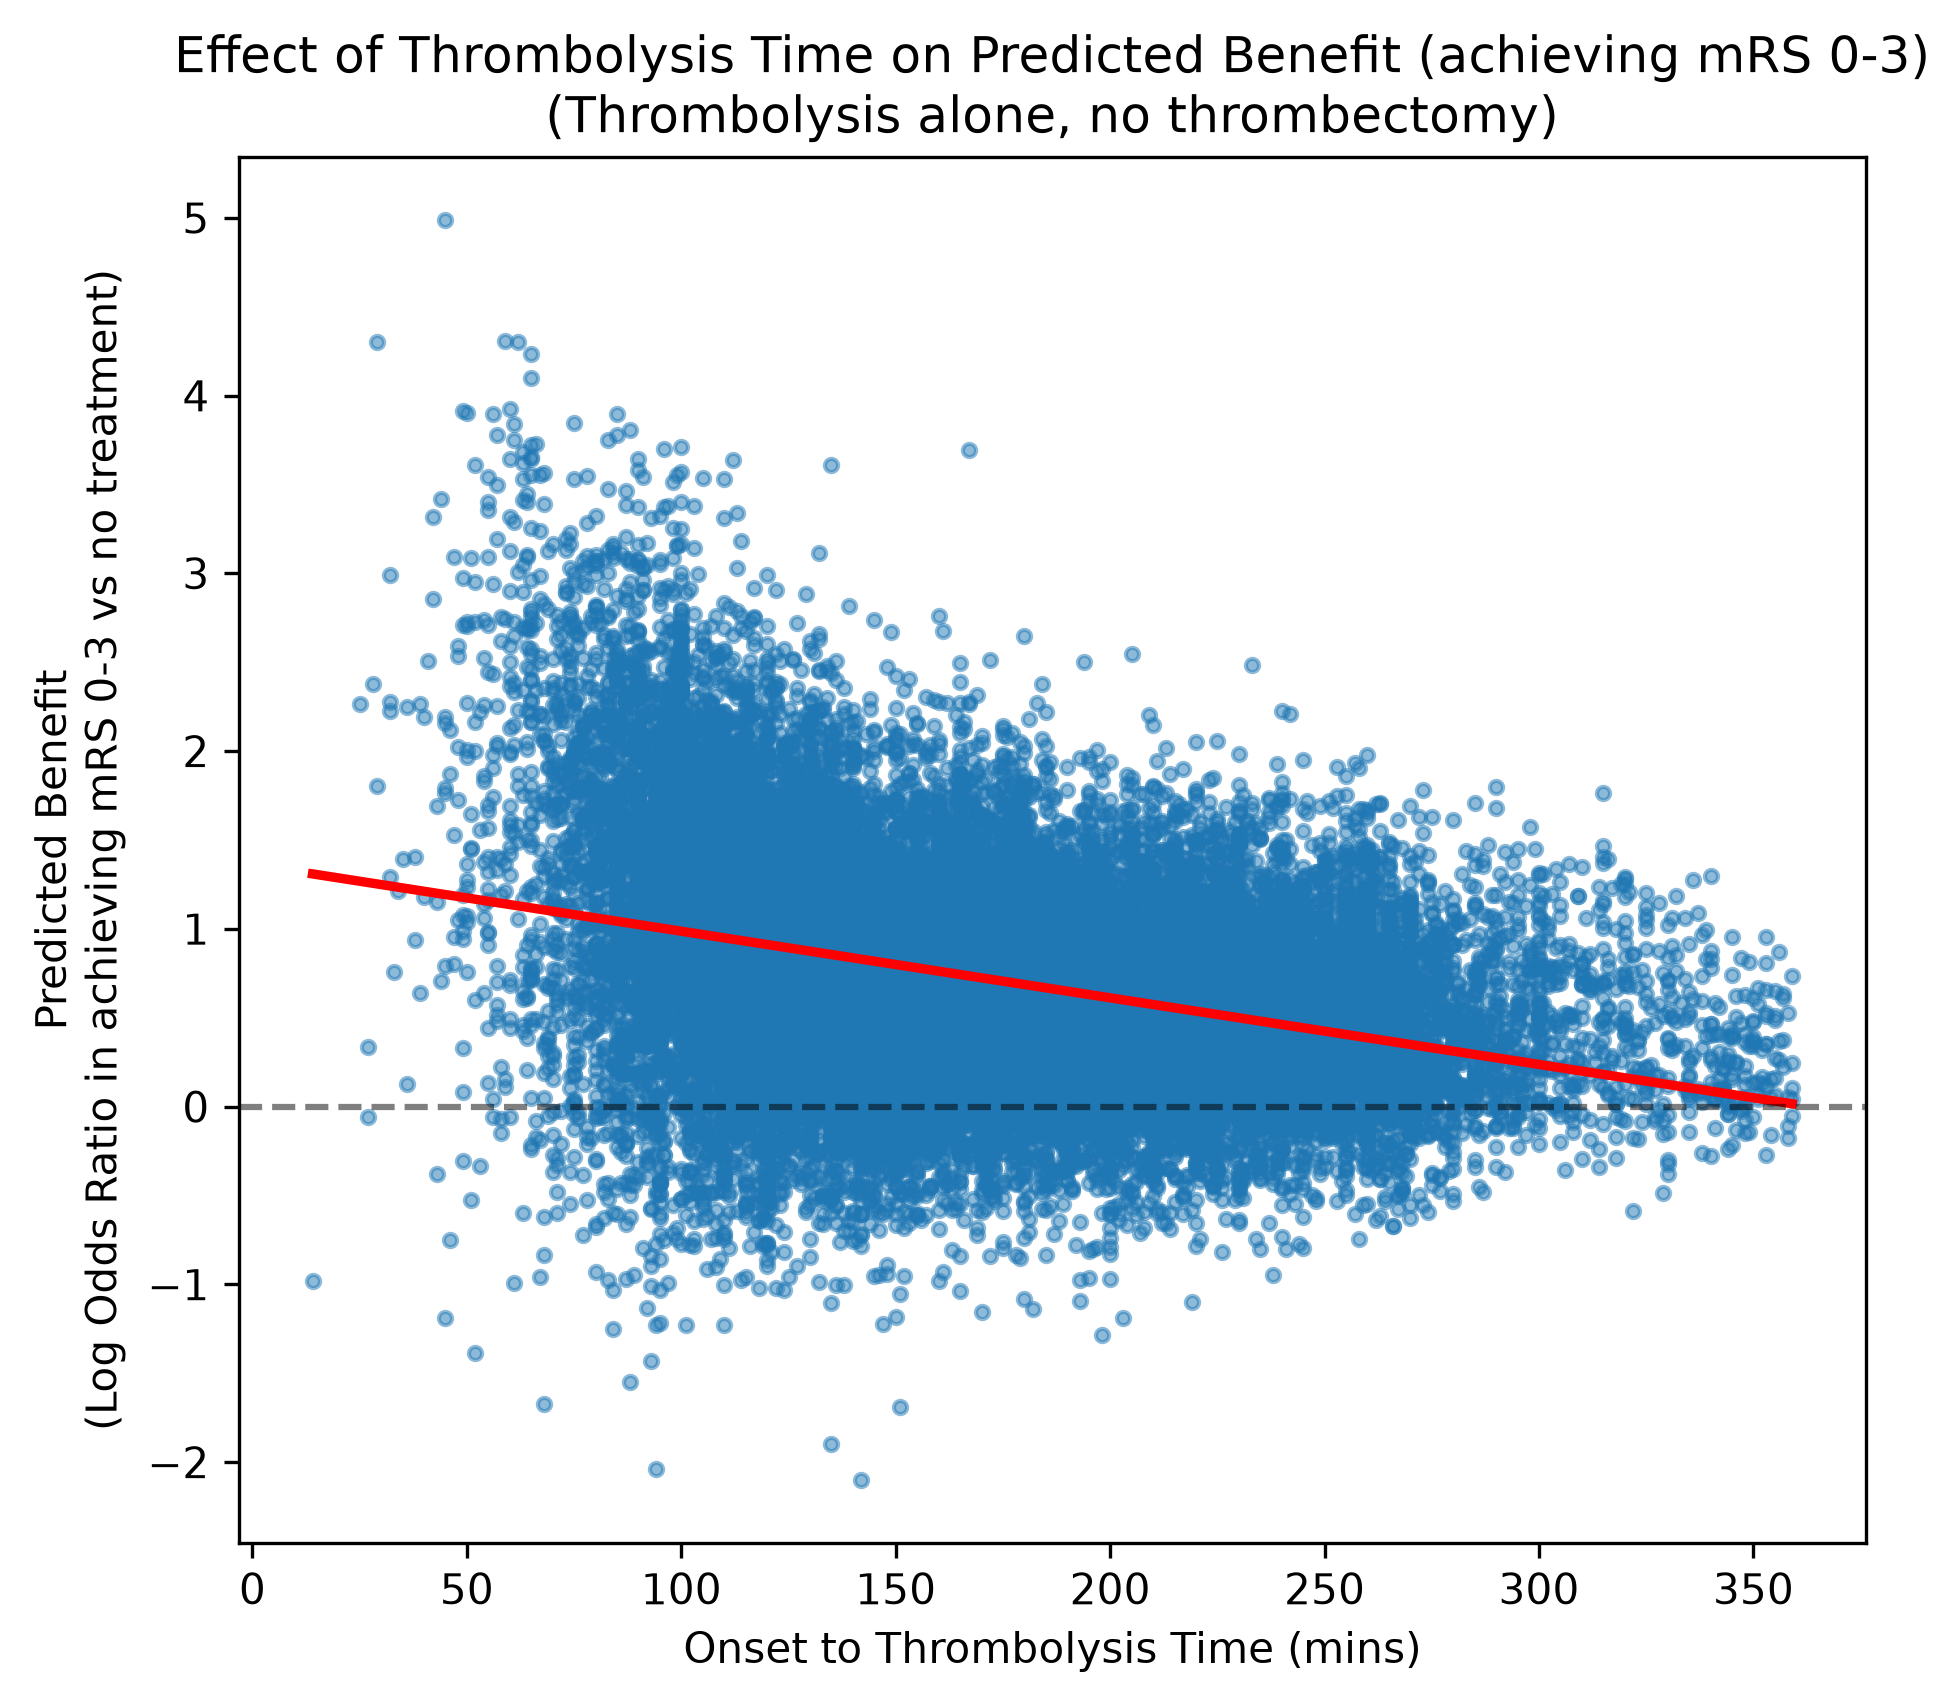
\includegraphics[width=\linewidth]{images/treatment_effects/thrombolysis_alone_time_effect_mrs_3.png}
        %\caption{}
        \label{fig:centre-left}
    \end{subfigure}
    %\hfill % Adds flexible horizontal spacing
    % Centre right image 
    \begin{subfigure}{0.38\textwidth}
        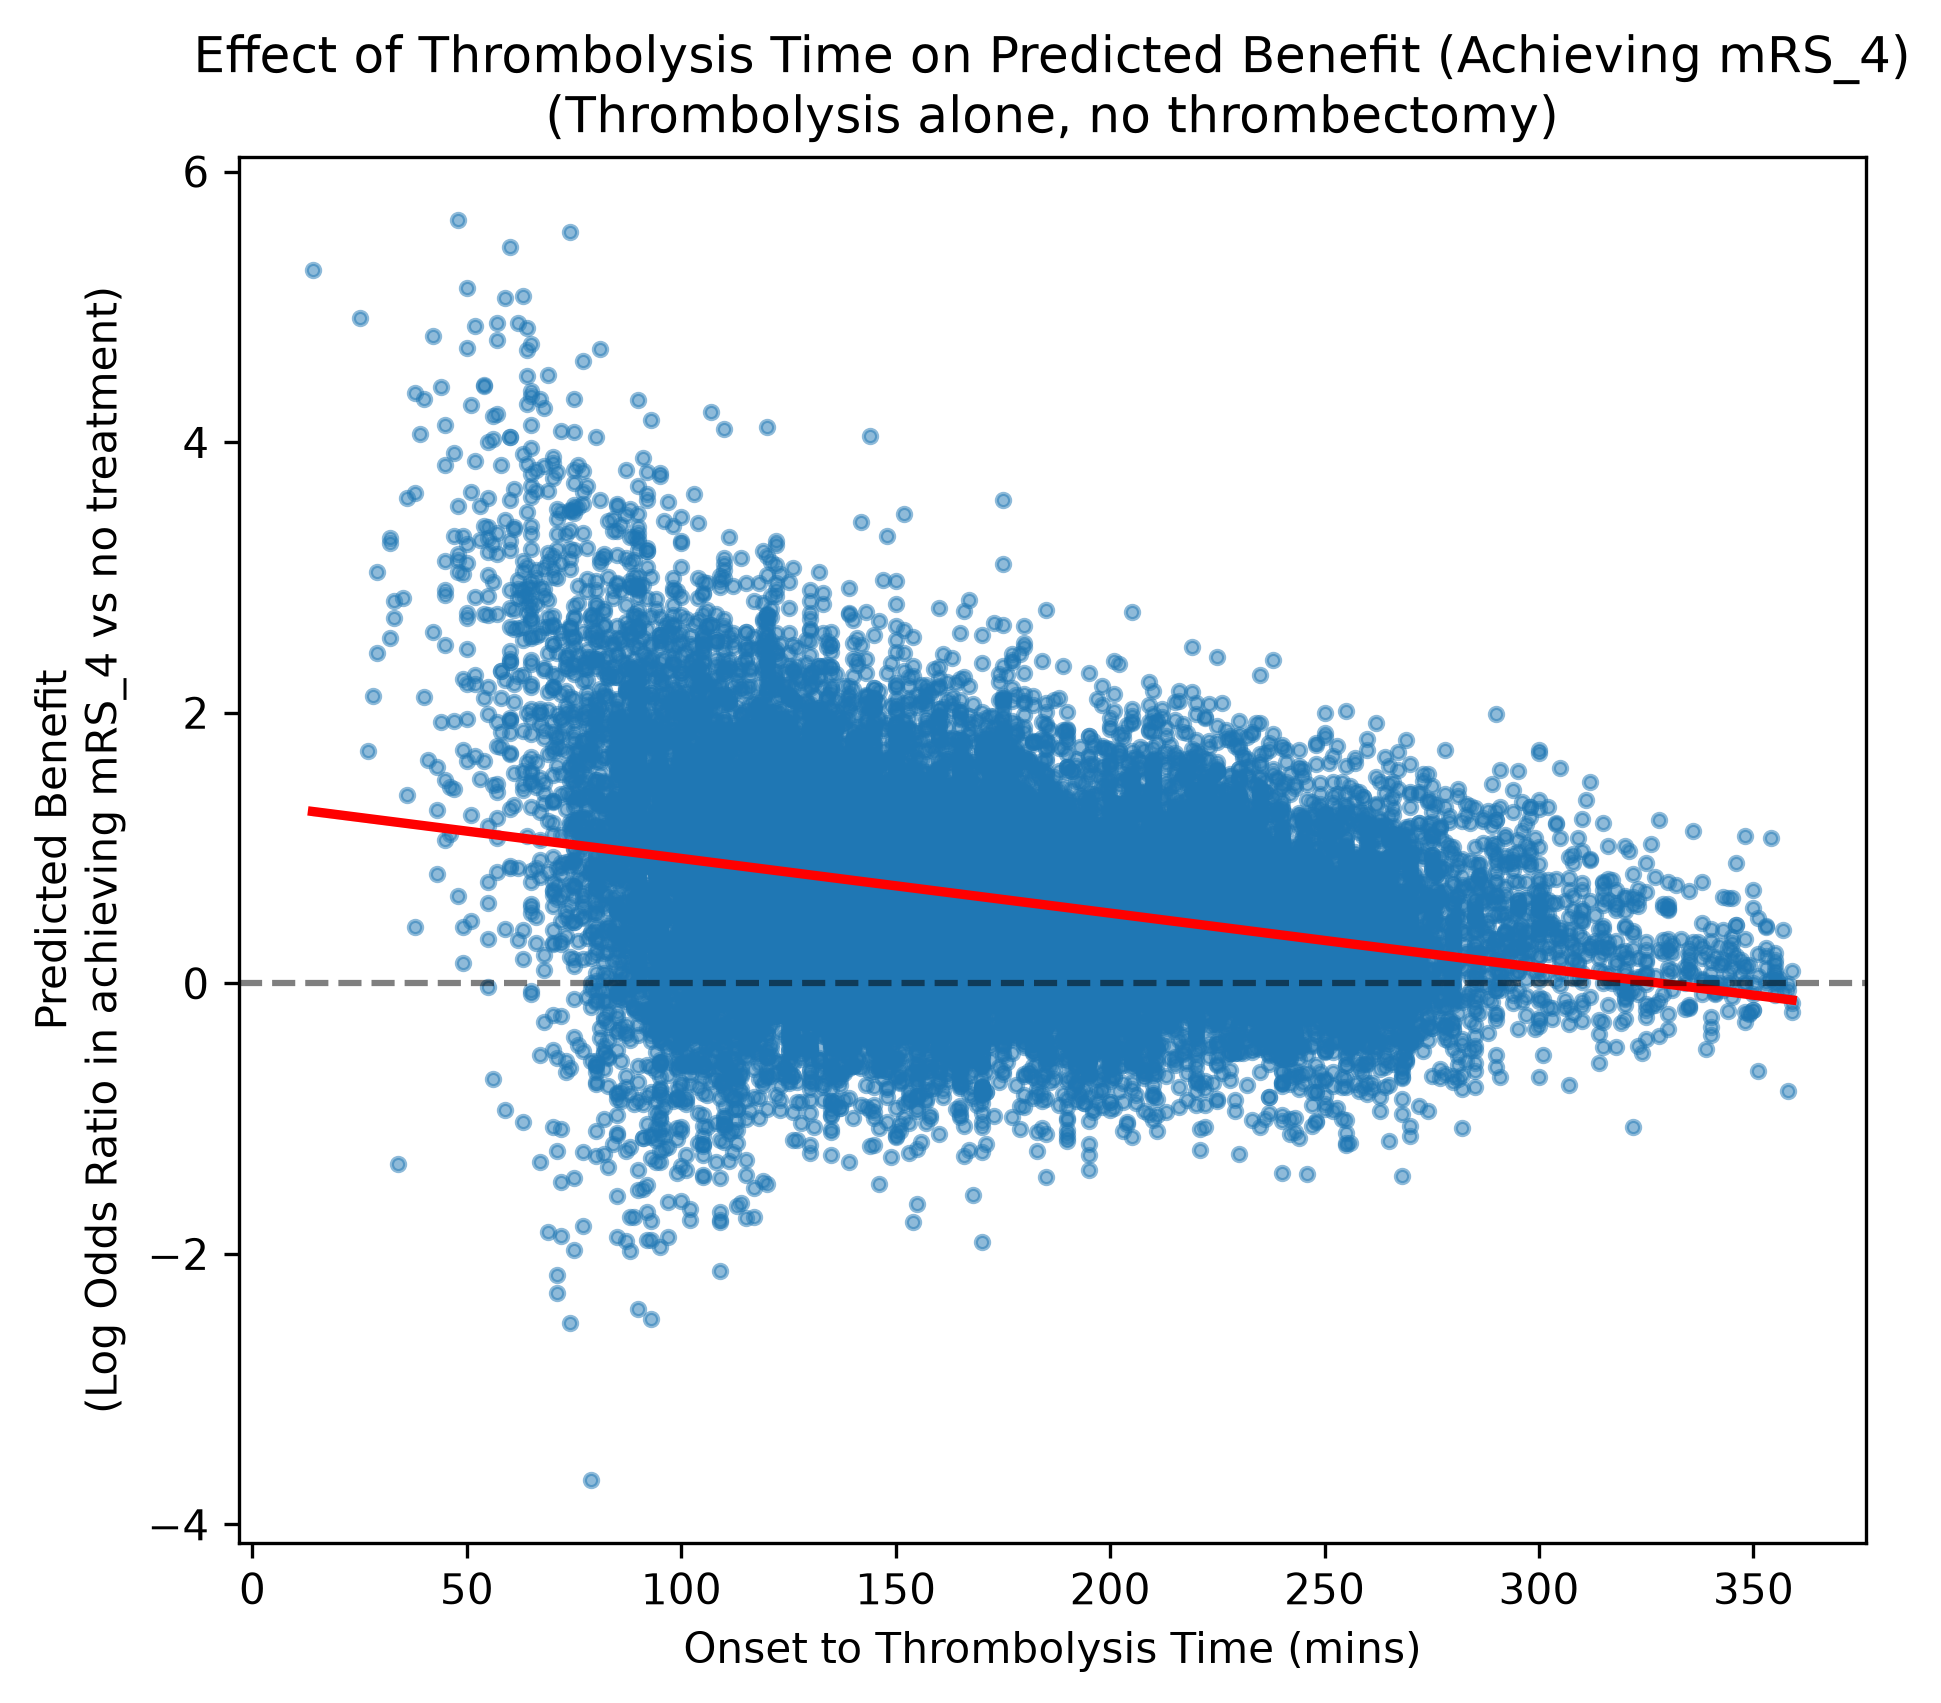
\includegraphics[width=\linewidth]{images/treatment_effects/thrombolysis_alone_time_effect_mrs_4.png}
        %\caption{}
        \label{fig:centre-right}
    \end{subfigure}

    \vspace{0.2cm} % Optional vertical space between rows

    % Bottom image
    \begin{subfigure}{0.38\textwidth}
        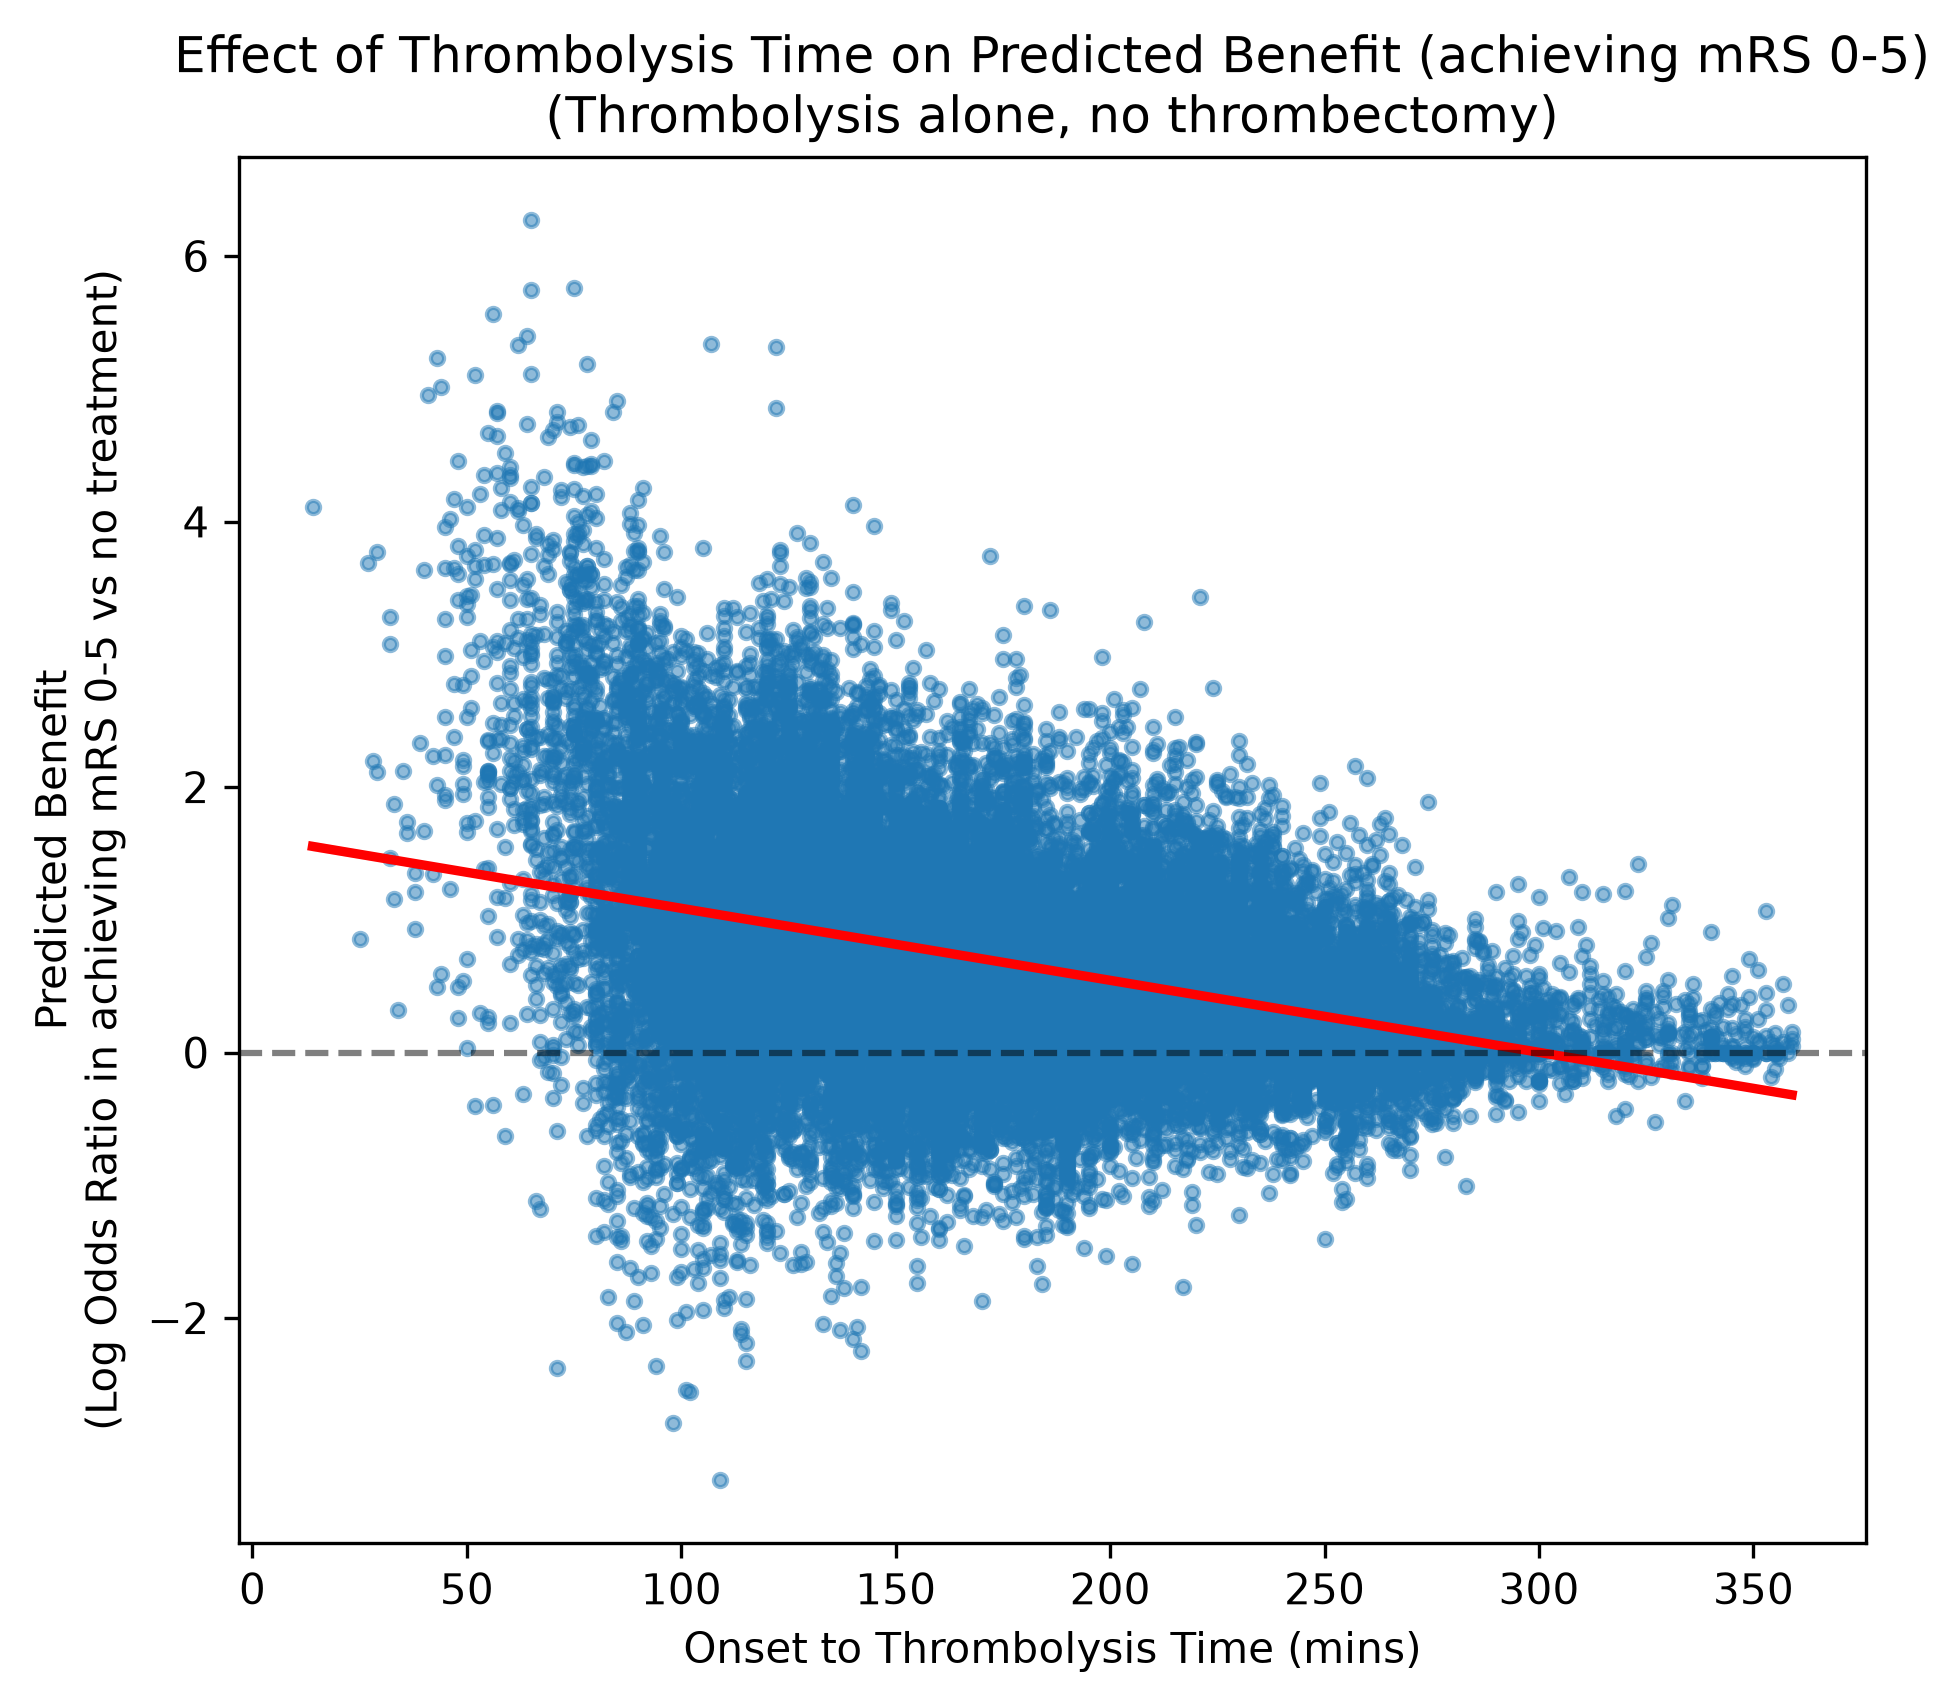
\includegraphics[width=\linewidth]{images/treatment_effects/thrombolysis_alone_time_effect_mrs_5}
        %\caption{}
        \label{fig:centre-right}
    \end{subfigure}
    
    \caption{Association between onset-to-thrombolysis time and individualised predicted benefit of thrombolysis alone, estimated using the S-learner XGBoost model. Each panel shows the predicted improvement in the odds of discharge at or below the specified modified Rankin Scale (mRS) threshold. Analyses are restricted to patients receiving intravenous thrombolysis without mechanical thrombectomy; each point represents an individual patient. The vertical axis shows the model-estimated treatment benefit on the log-odds scale, relative to the counterfactual prediction under no treatment. The red line denotes the fitted linear trend, illustrating the decline in predicted benefit with increasing onset-to-thrombolysis time. The dashed horizontal line indicates no predicted treatment benefit (log-odds ratio = 0); values above and below this line indicate predicted benefit and harm, respectively.}
    \label{fig:s_learner_time_thrombolysis}
\end{figure}


%%%%%%%%%%%%%%%%%%%%%%%%%%%%%%%%%%%%%%%%%%

Figure \ref{fig:s_learner_time_thrombectomy} shows a scatter plot, with regression line, of of the estimated benefit of thrombectomy (log odds ratio, treated vs untreated), by time after onset, in achieving each mRS threshold. This model used actual onset-to-treatment times for thrombectomy, and is for patients receiving thrombectomy only.


\begin{figure}[htbp]
    \centering
    
    % Top left
    \begin{subfigure}{0.38\textwidth}
        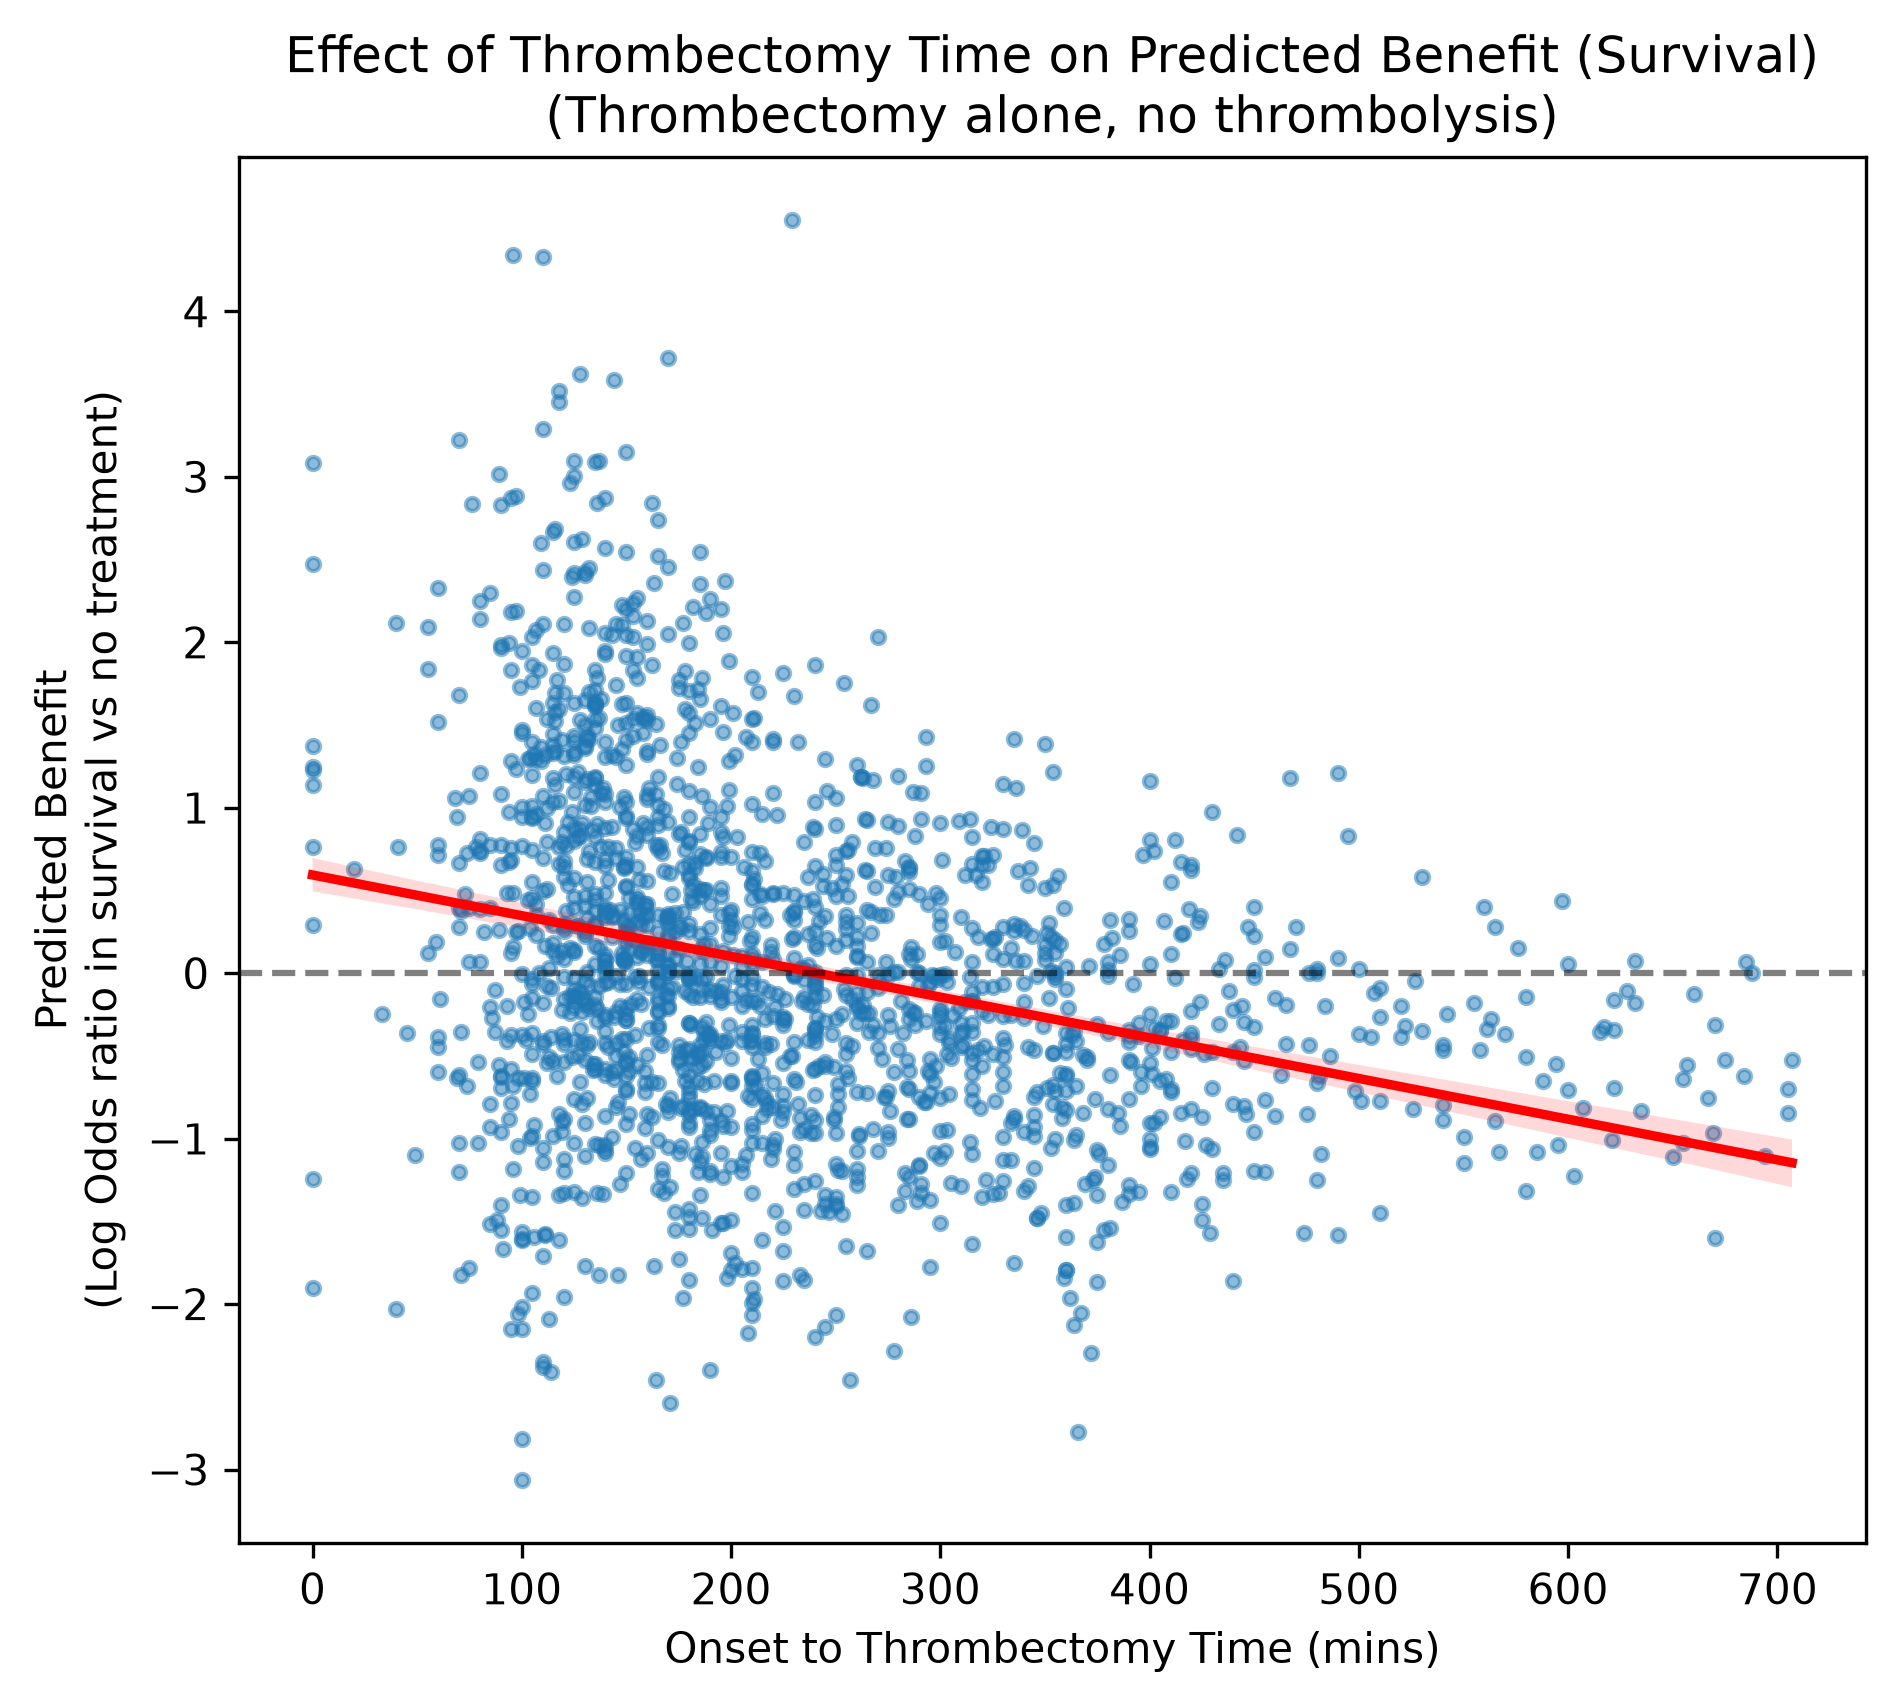
\includegraphics[width=\linewidth]{images/treatment_effects/thrombectomy_alone_time_effect_mrs_1.png}
        %\caption{}
        \label{fig:top-left}
    \end{subfigure}
    %\hfill % Adds flexible horizontal spacing
    % top right image 
    \begin{subfigure}{0.38\textwidth}
        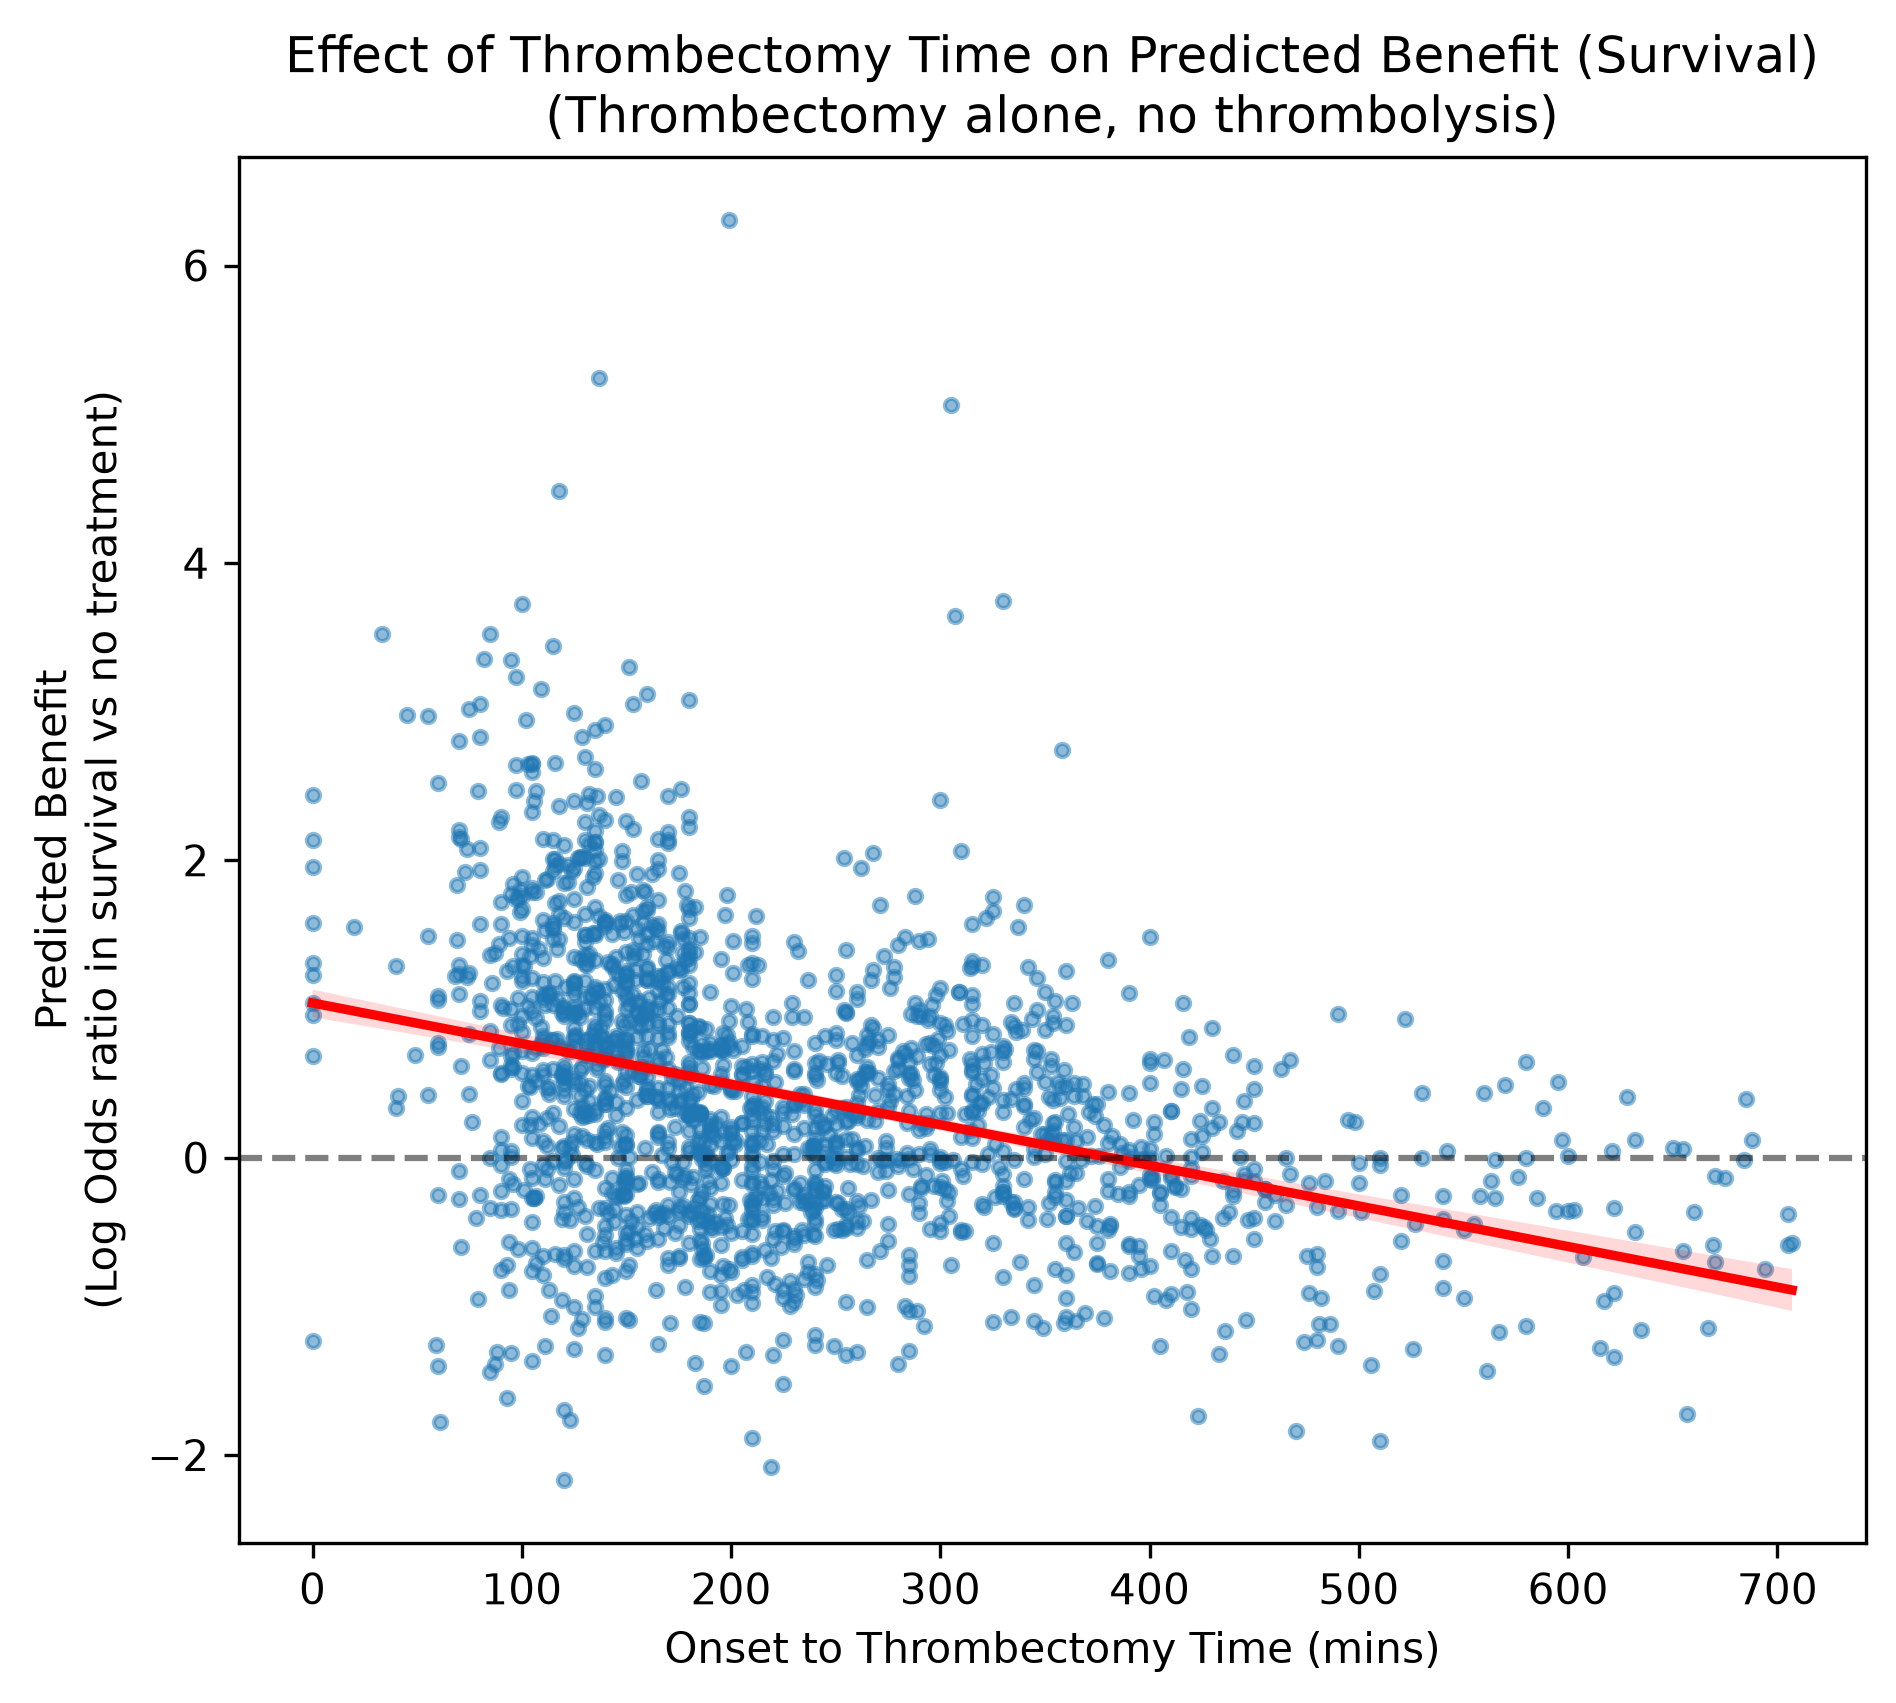
\includegraphics[width=\linewidth]{images/treatment_effects/thrombectomy_alone_time_effect_mrs_2.png}
        %\caption{}
        \label{fig:bottom-left}
    \end{subfigure}

    \vspace{0.2cm} % Optional vertical space between rows

    % Center left image
    \begin{subfigure}{0.38\textwidth}
        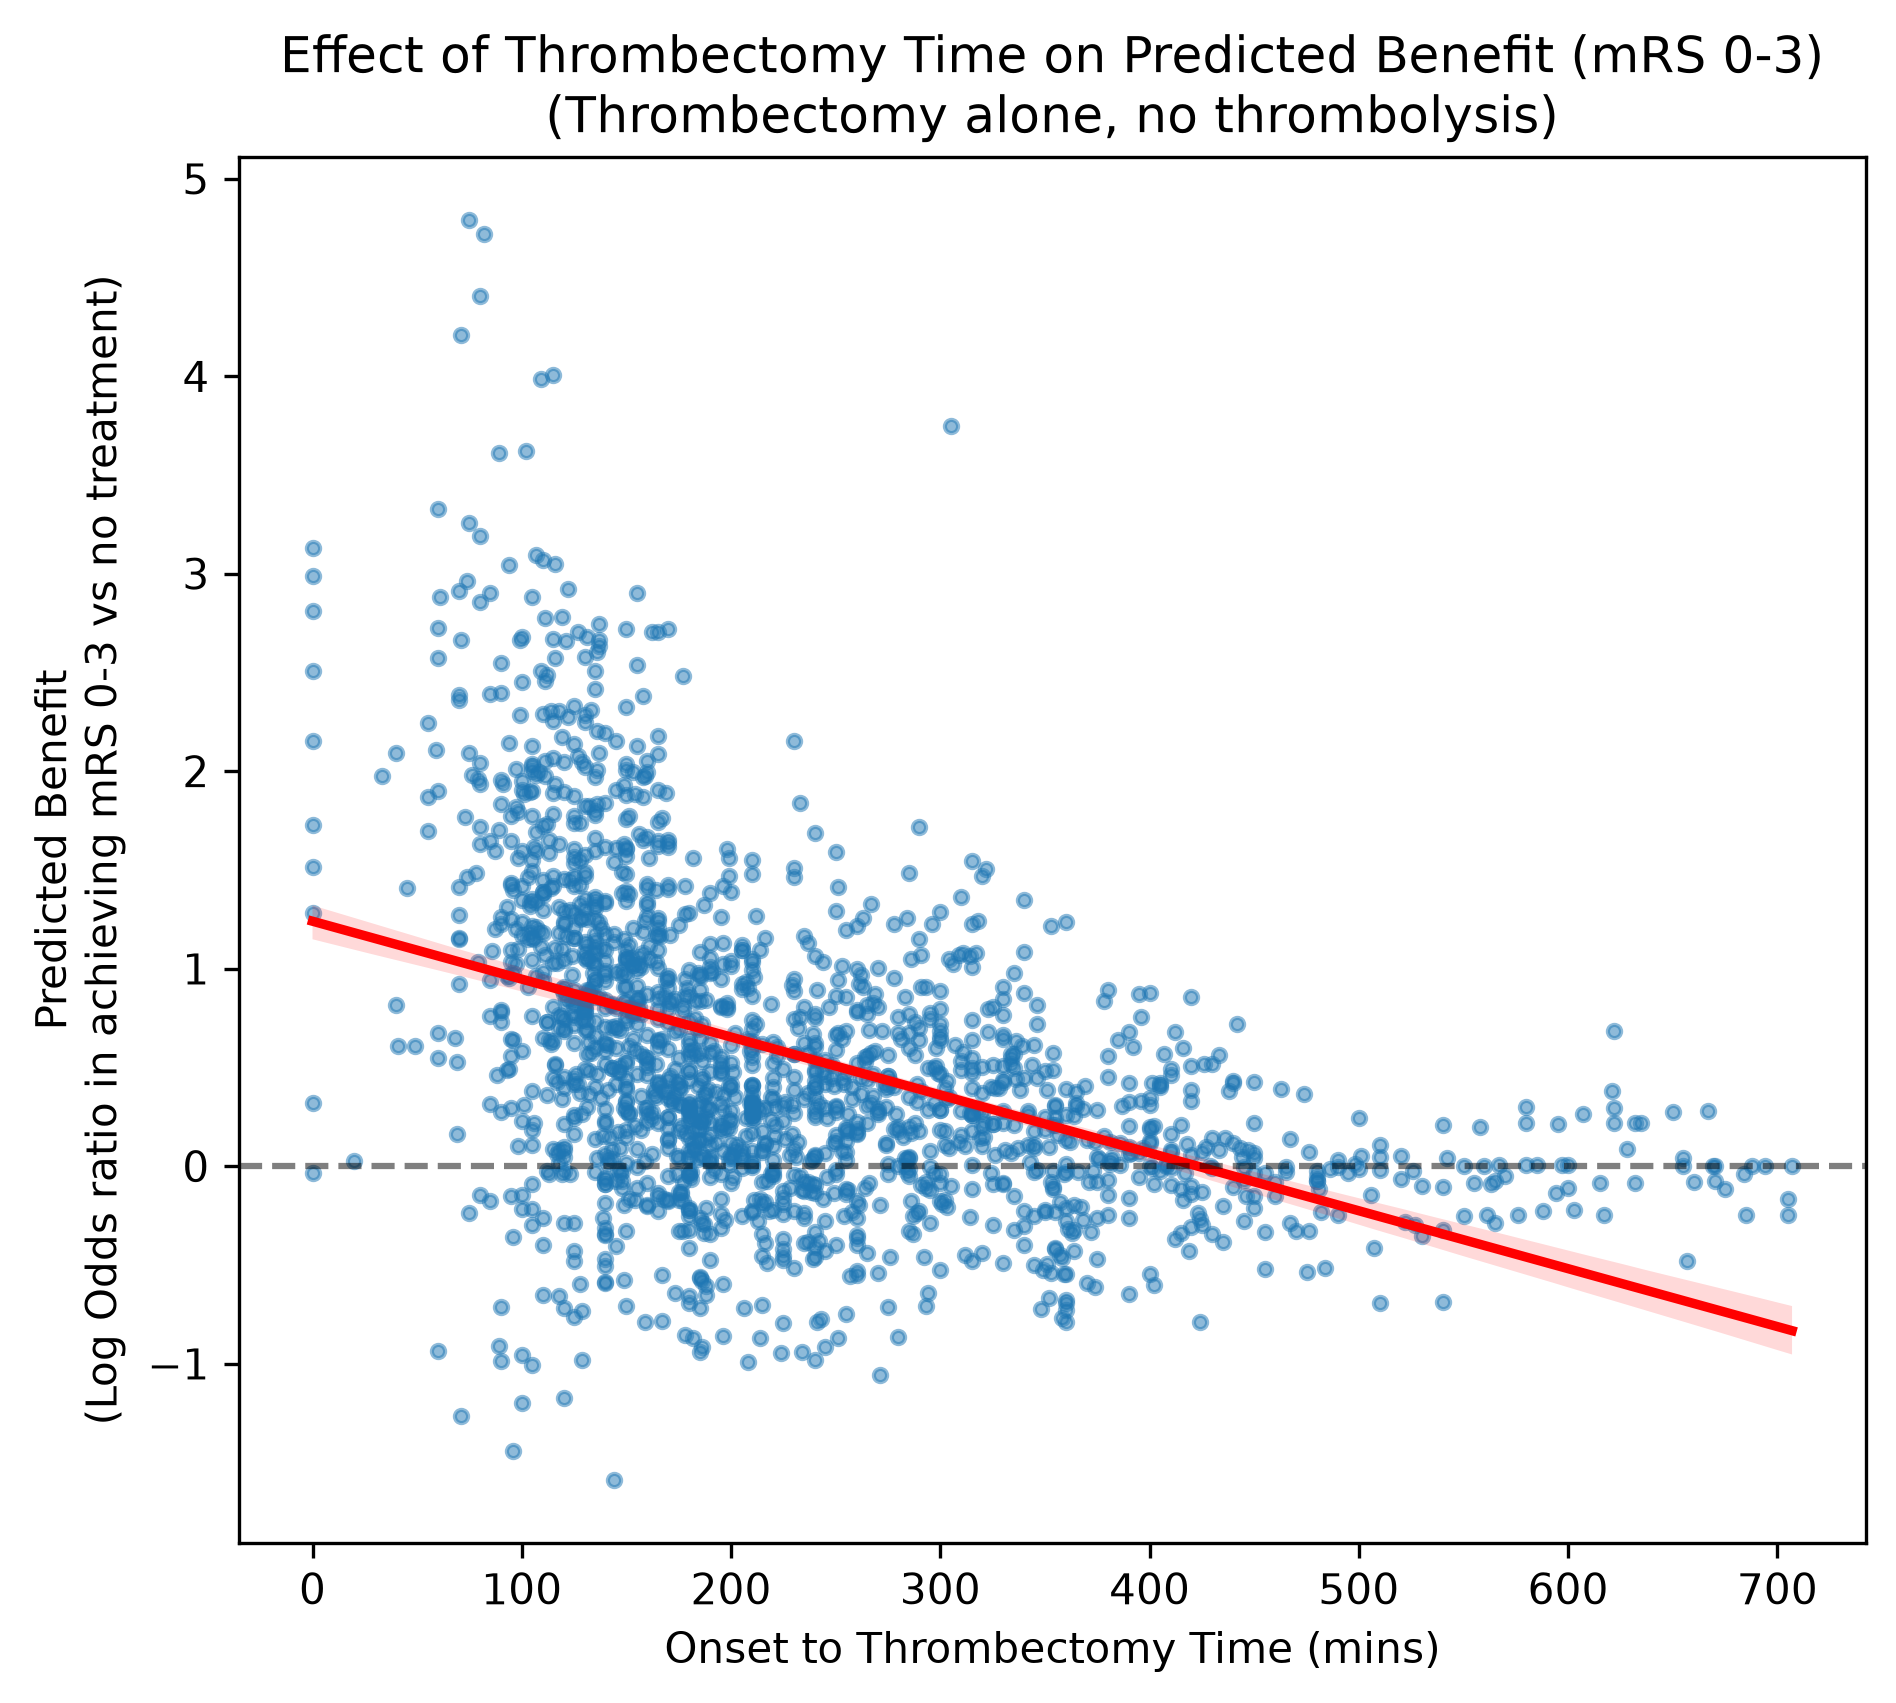
\includegraphics[width=\linewidth]{images/treatment_effects/thrombectomy_alone_time_effect_mrs_3.png}
        %\caption{}
        \label{fig:centre-left}
    \end{subfigure}
    %\hfill{} % Adds flexible horizontal spacing
    % Centre right image 
    \begin{subfigure}{0.38\textwidth}
        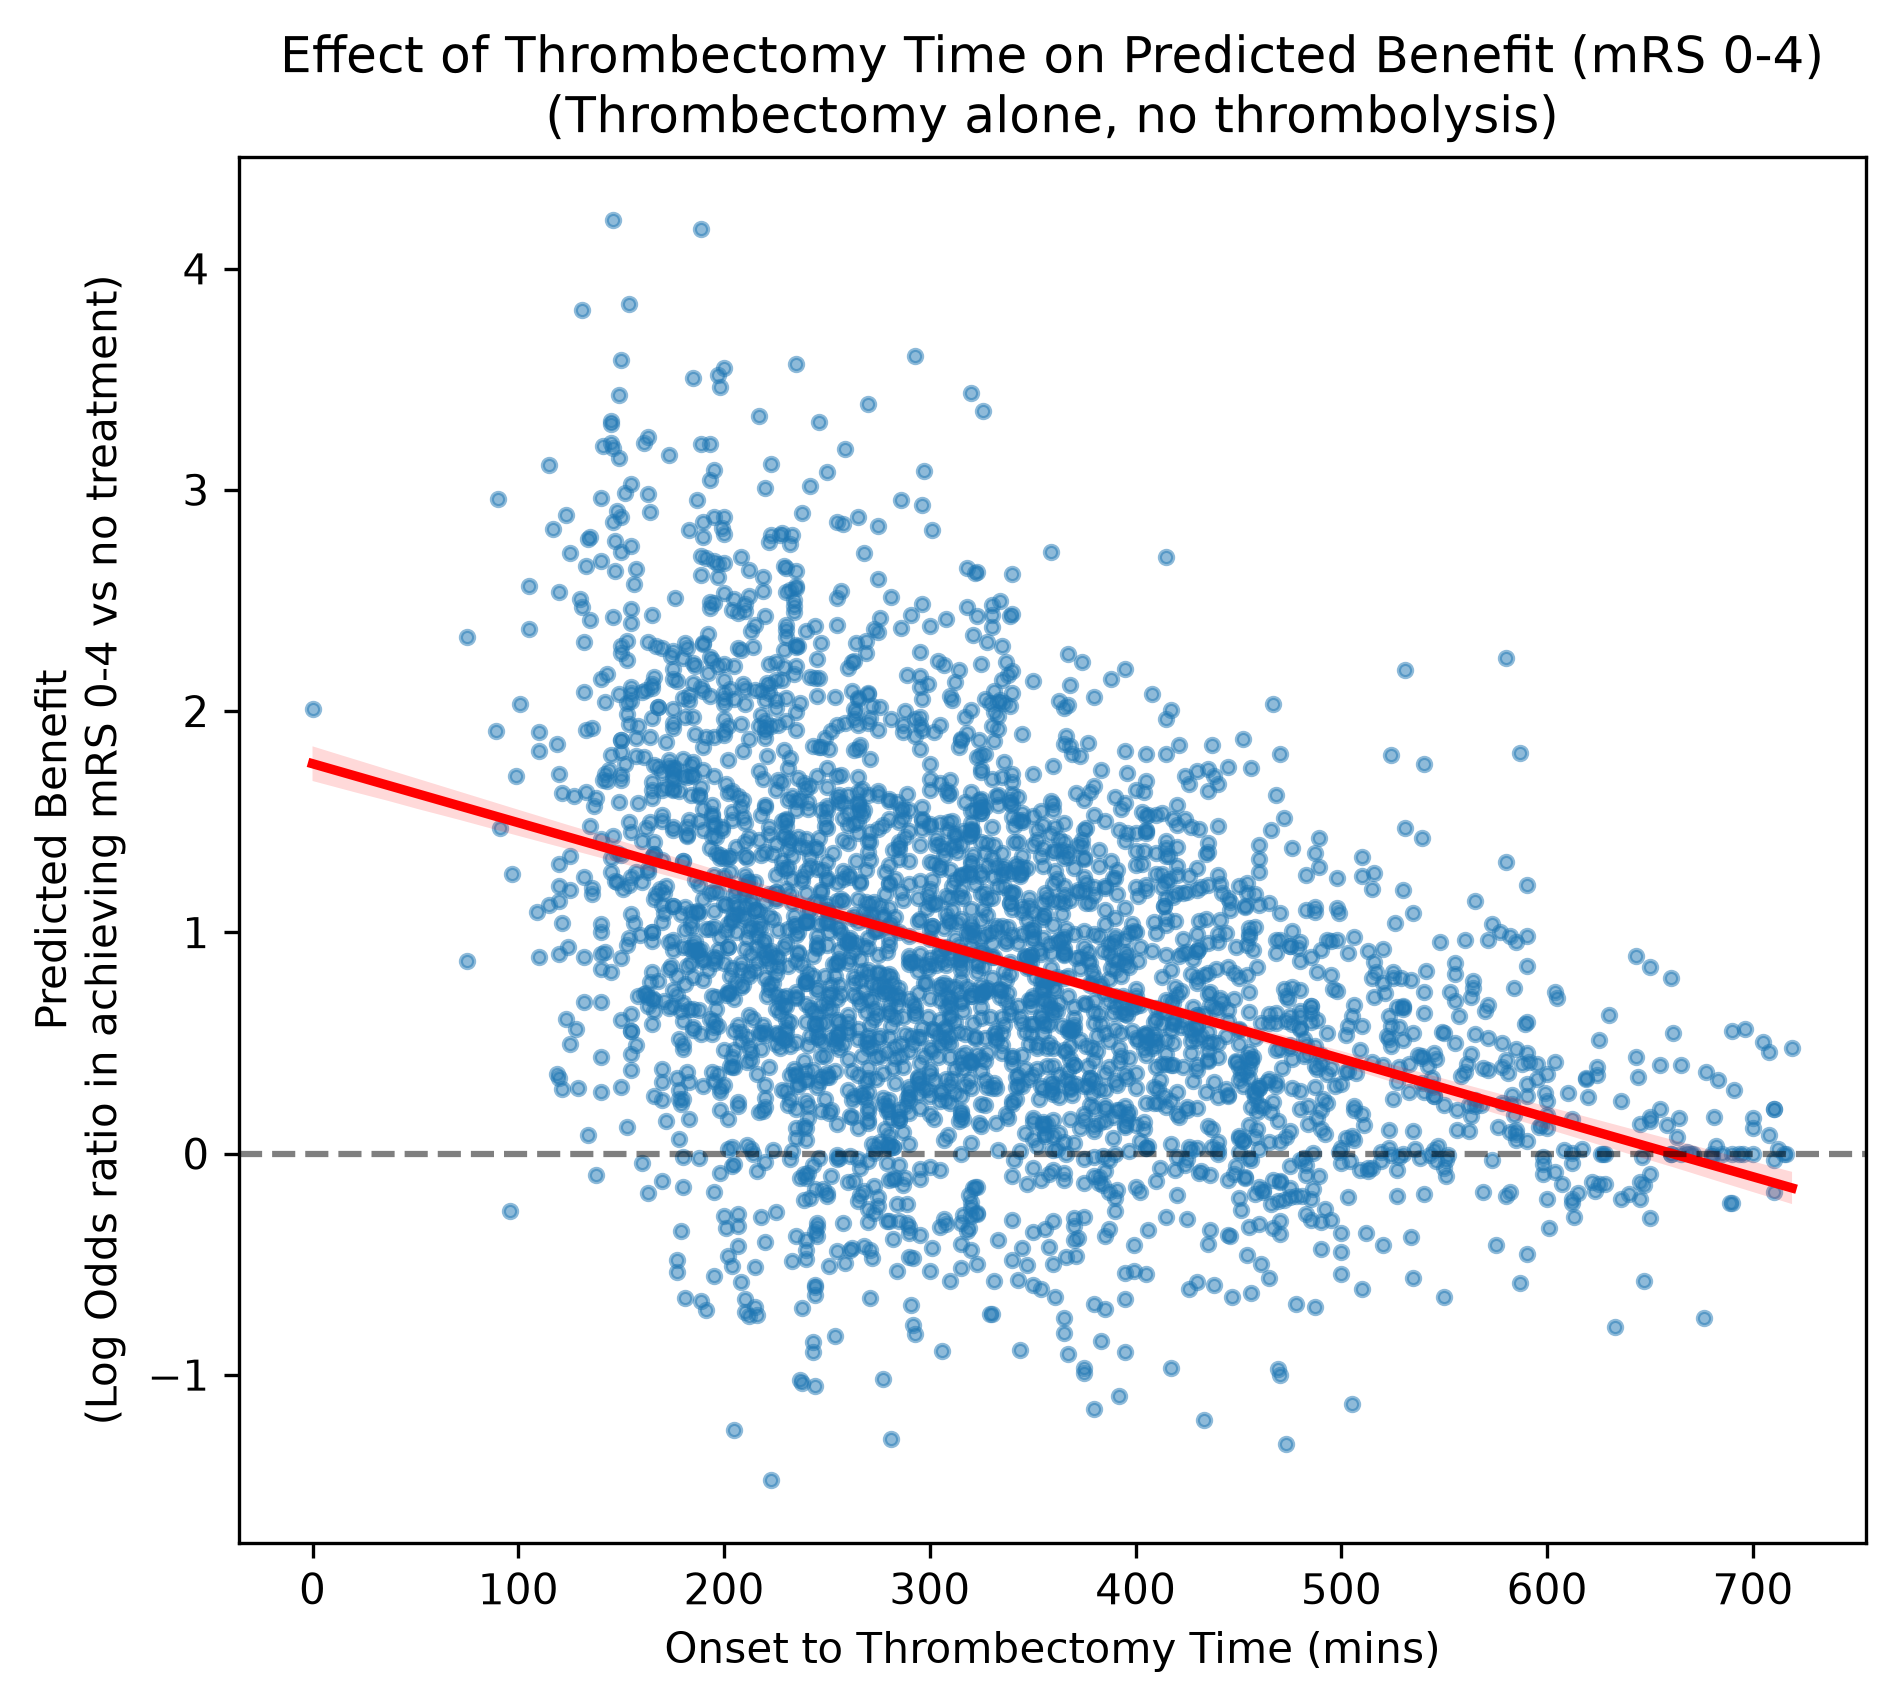
\includegraphics[width=\linewidth]{images/treatment_effects/thrombectomy_alone_time_effect_mrs_4.png}
        %\caption{}
        \label{fig:centre-right}
    \end{subfigure}

    \vspace{0.2cm} % Optional vertical space between rows

    % Bottom image
    \begin{subfigure}{0.38\textwidth}
        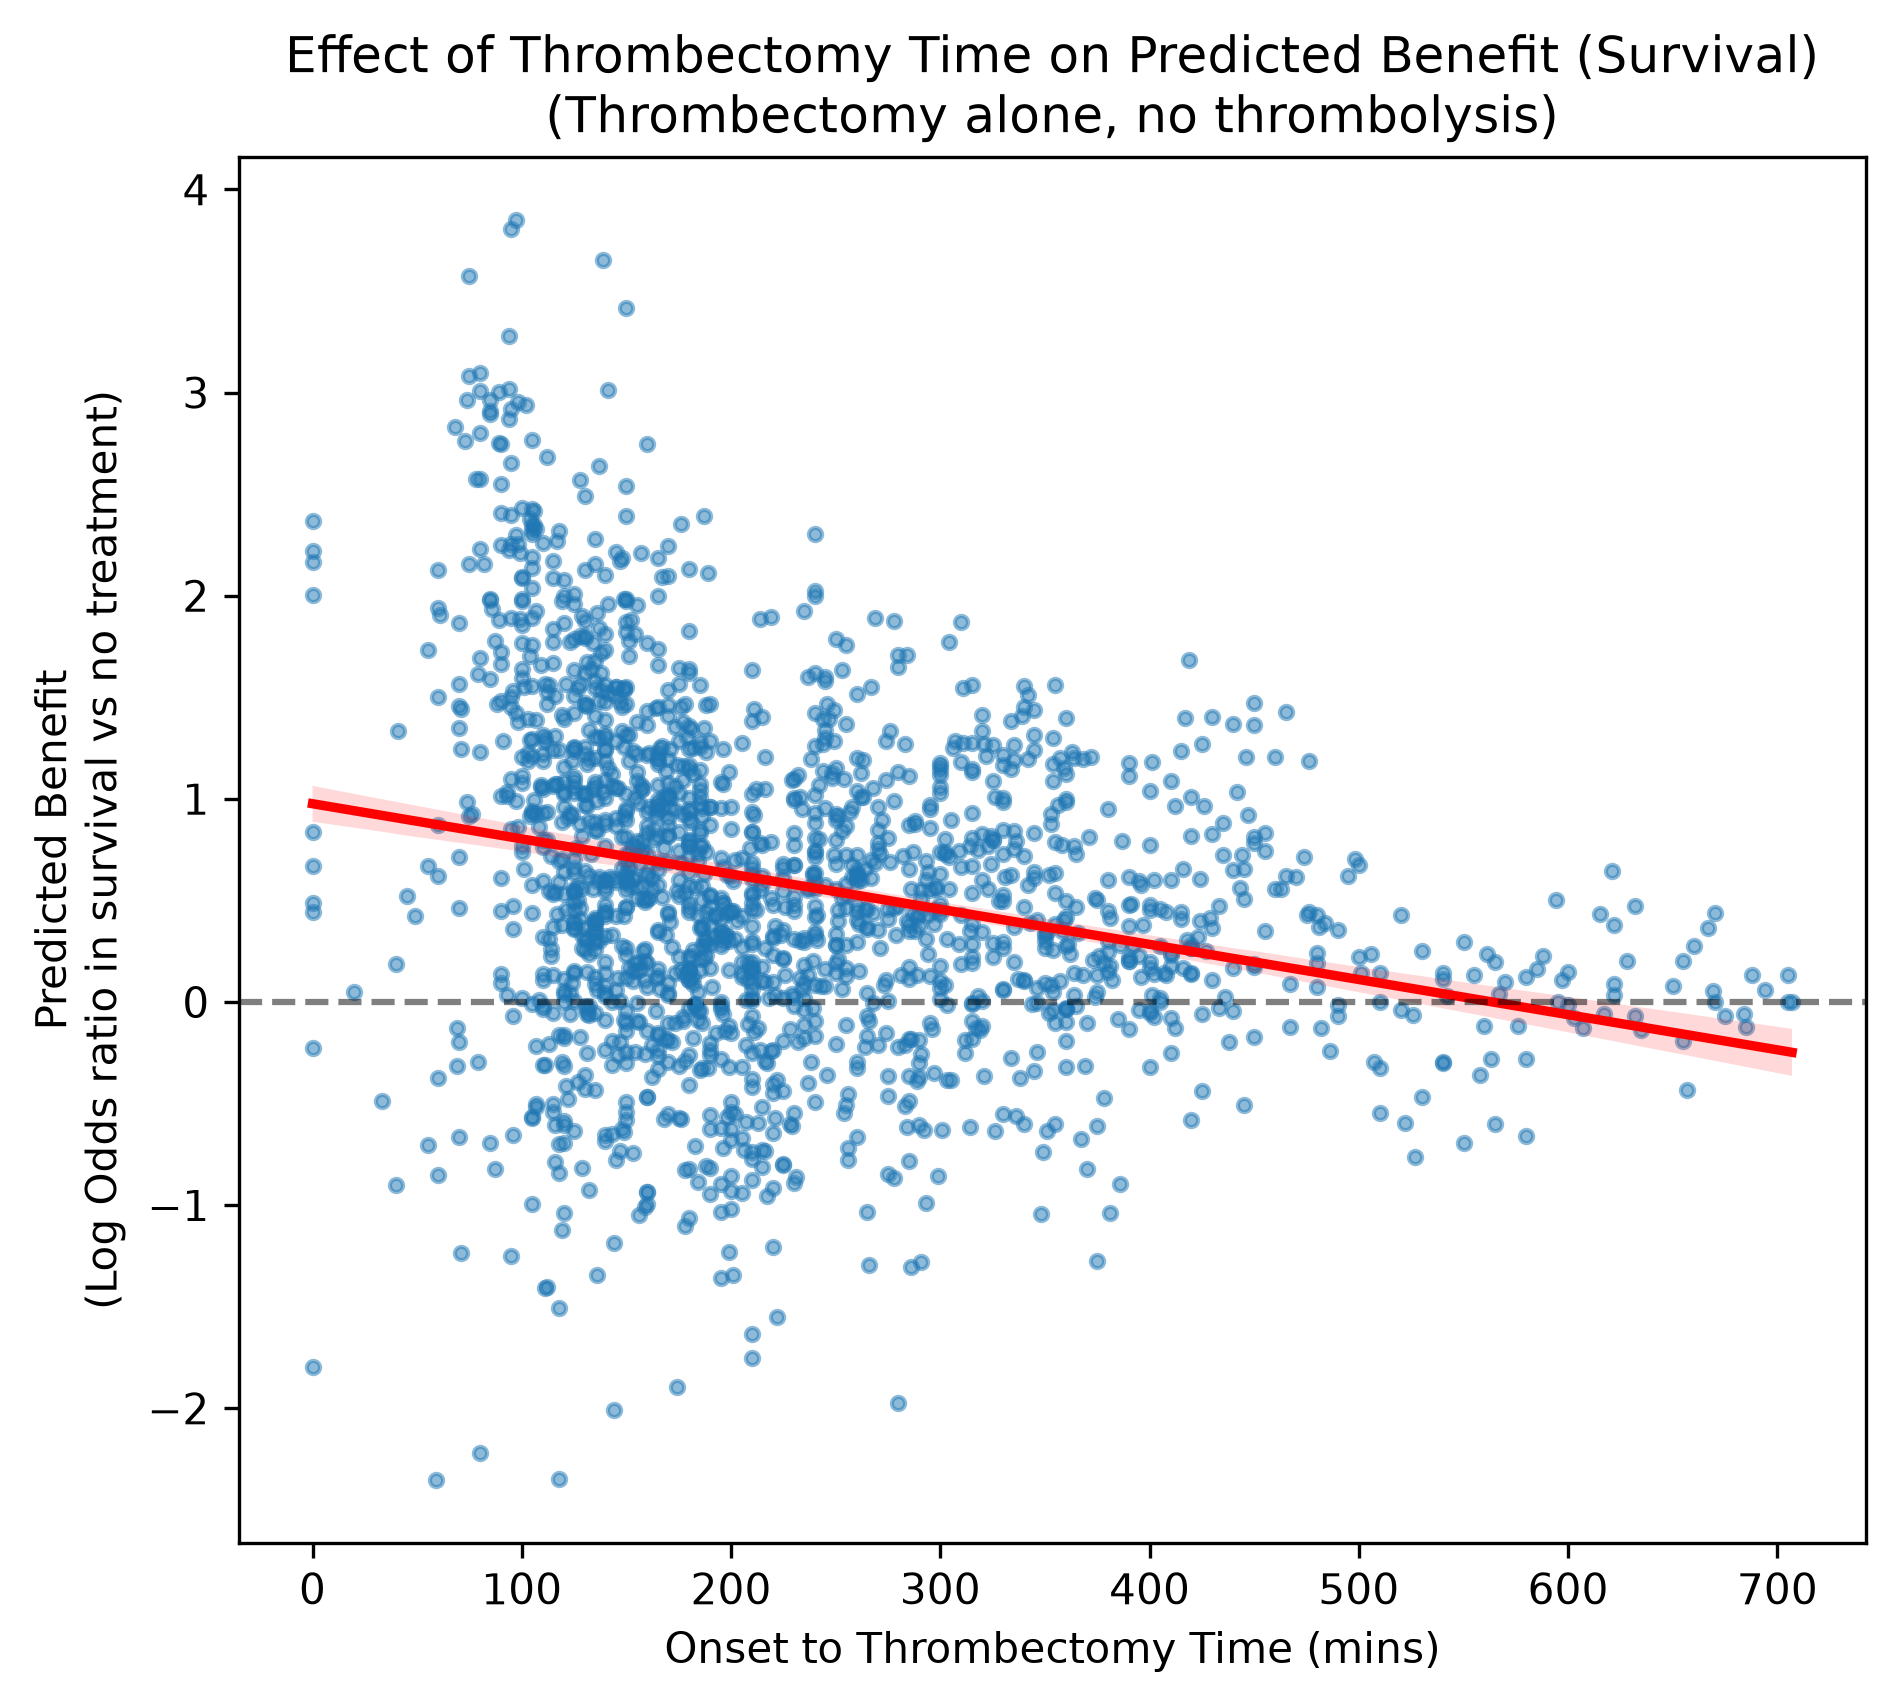
\includegraphics[width=\linewidth]{images/treatment_effects/thrombectomy_alone_time_effect_mrs_5}
        %\caption{}
        \label{fig:centre-right}
    \end{subfigure}
    
    \caption{Association between onset-to-thrombectomy time and individualised predicted benefit of thrombectomy alone, estimated using the S-learner XGBoost model. Each panel shows the predicted improvement in the odds of discharge at or below the specified modified Rankin Scale (mRS) threshold. Analyses are restricted to patients receiving mechanical thrombectomy without intravenous thrombolysis; each point represents an individual patient. The vertical axis shows the model-estimated treatment benefit on the log-odds scale, relative to the counterfactual prediction under no treatment. The red line denotes the fitted linear trend, illustrating the decline in predicted benefit with increasing onset-to-thrombectomy time. The dashed horizontal line indicates no predicted treatment benefit (log-odds ratio = 0); values above and below this line indicate predicted benefit and harm, respectively.}
    \label{fig:s_learner_time_thrombectomy}
\end{figure}


% ################### CASUAL FOREST ###########################

\newpage

\subsection{Causal Forest}

Figure \ref{fig:causal_forest_benefit} shows treatment effect estimates, estimated using an orthogonal Causal Forest, for achieving each possible mRS threshold. Treatment effects are shown as Conditional Average Treatment effects (CATE), which is the change in absolute percentage probability of achieving the desired outcome. Treatment type and speed (early vs late, using a 270 min onset-to-treatment threshold) were coded as a categorical value for this model.

\begin{figure}
    \centering
    
    % Top left
    \begin{subfigure}{0.49\textwidth}
        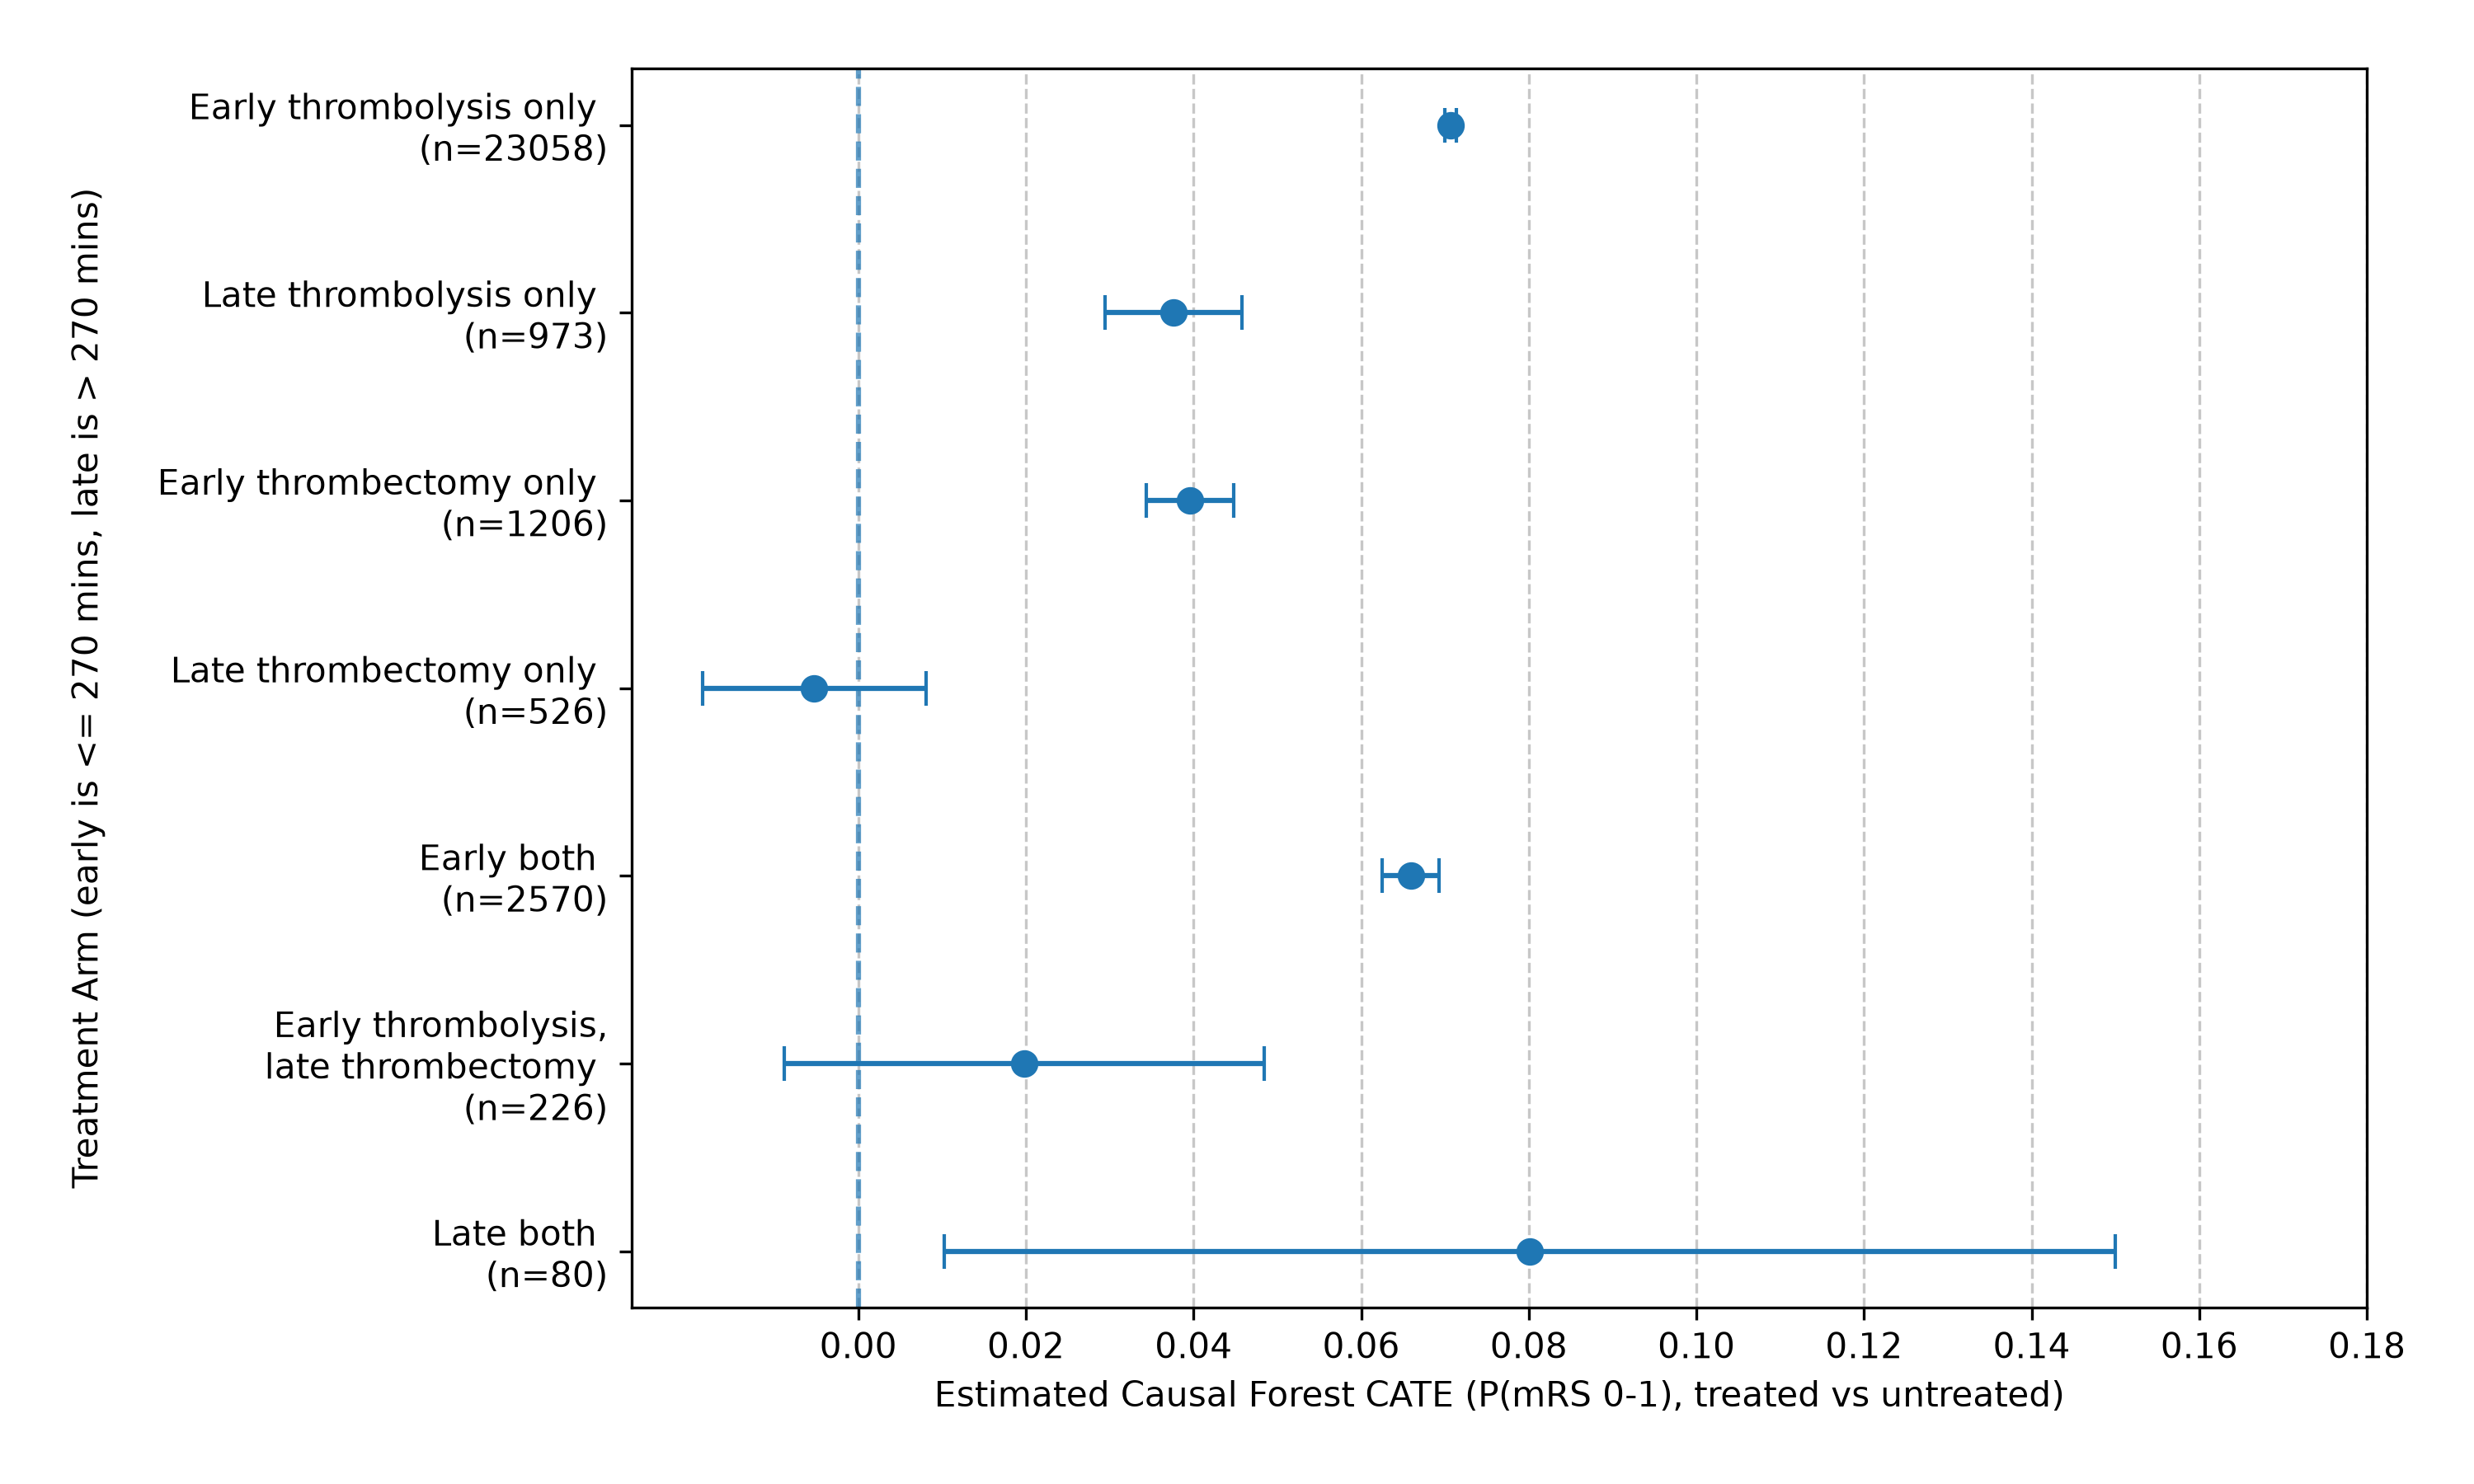
\includegraphics[width=\linewidth]{images/treatment_effects/causal_forest_counterfactual_cate_estimates_1.png}
        %\caption{}
        \label{fig:top-left}
    \end{subfigure}
    \hfill % Adds flexible horizontal spacing
    % top right image 
    \begin{subfigure}{0.49\textwidth}
        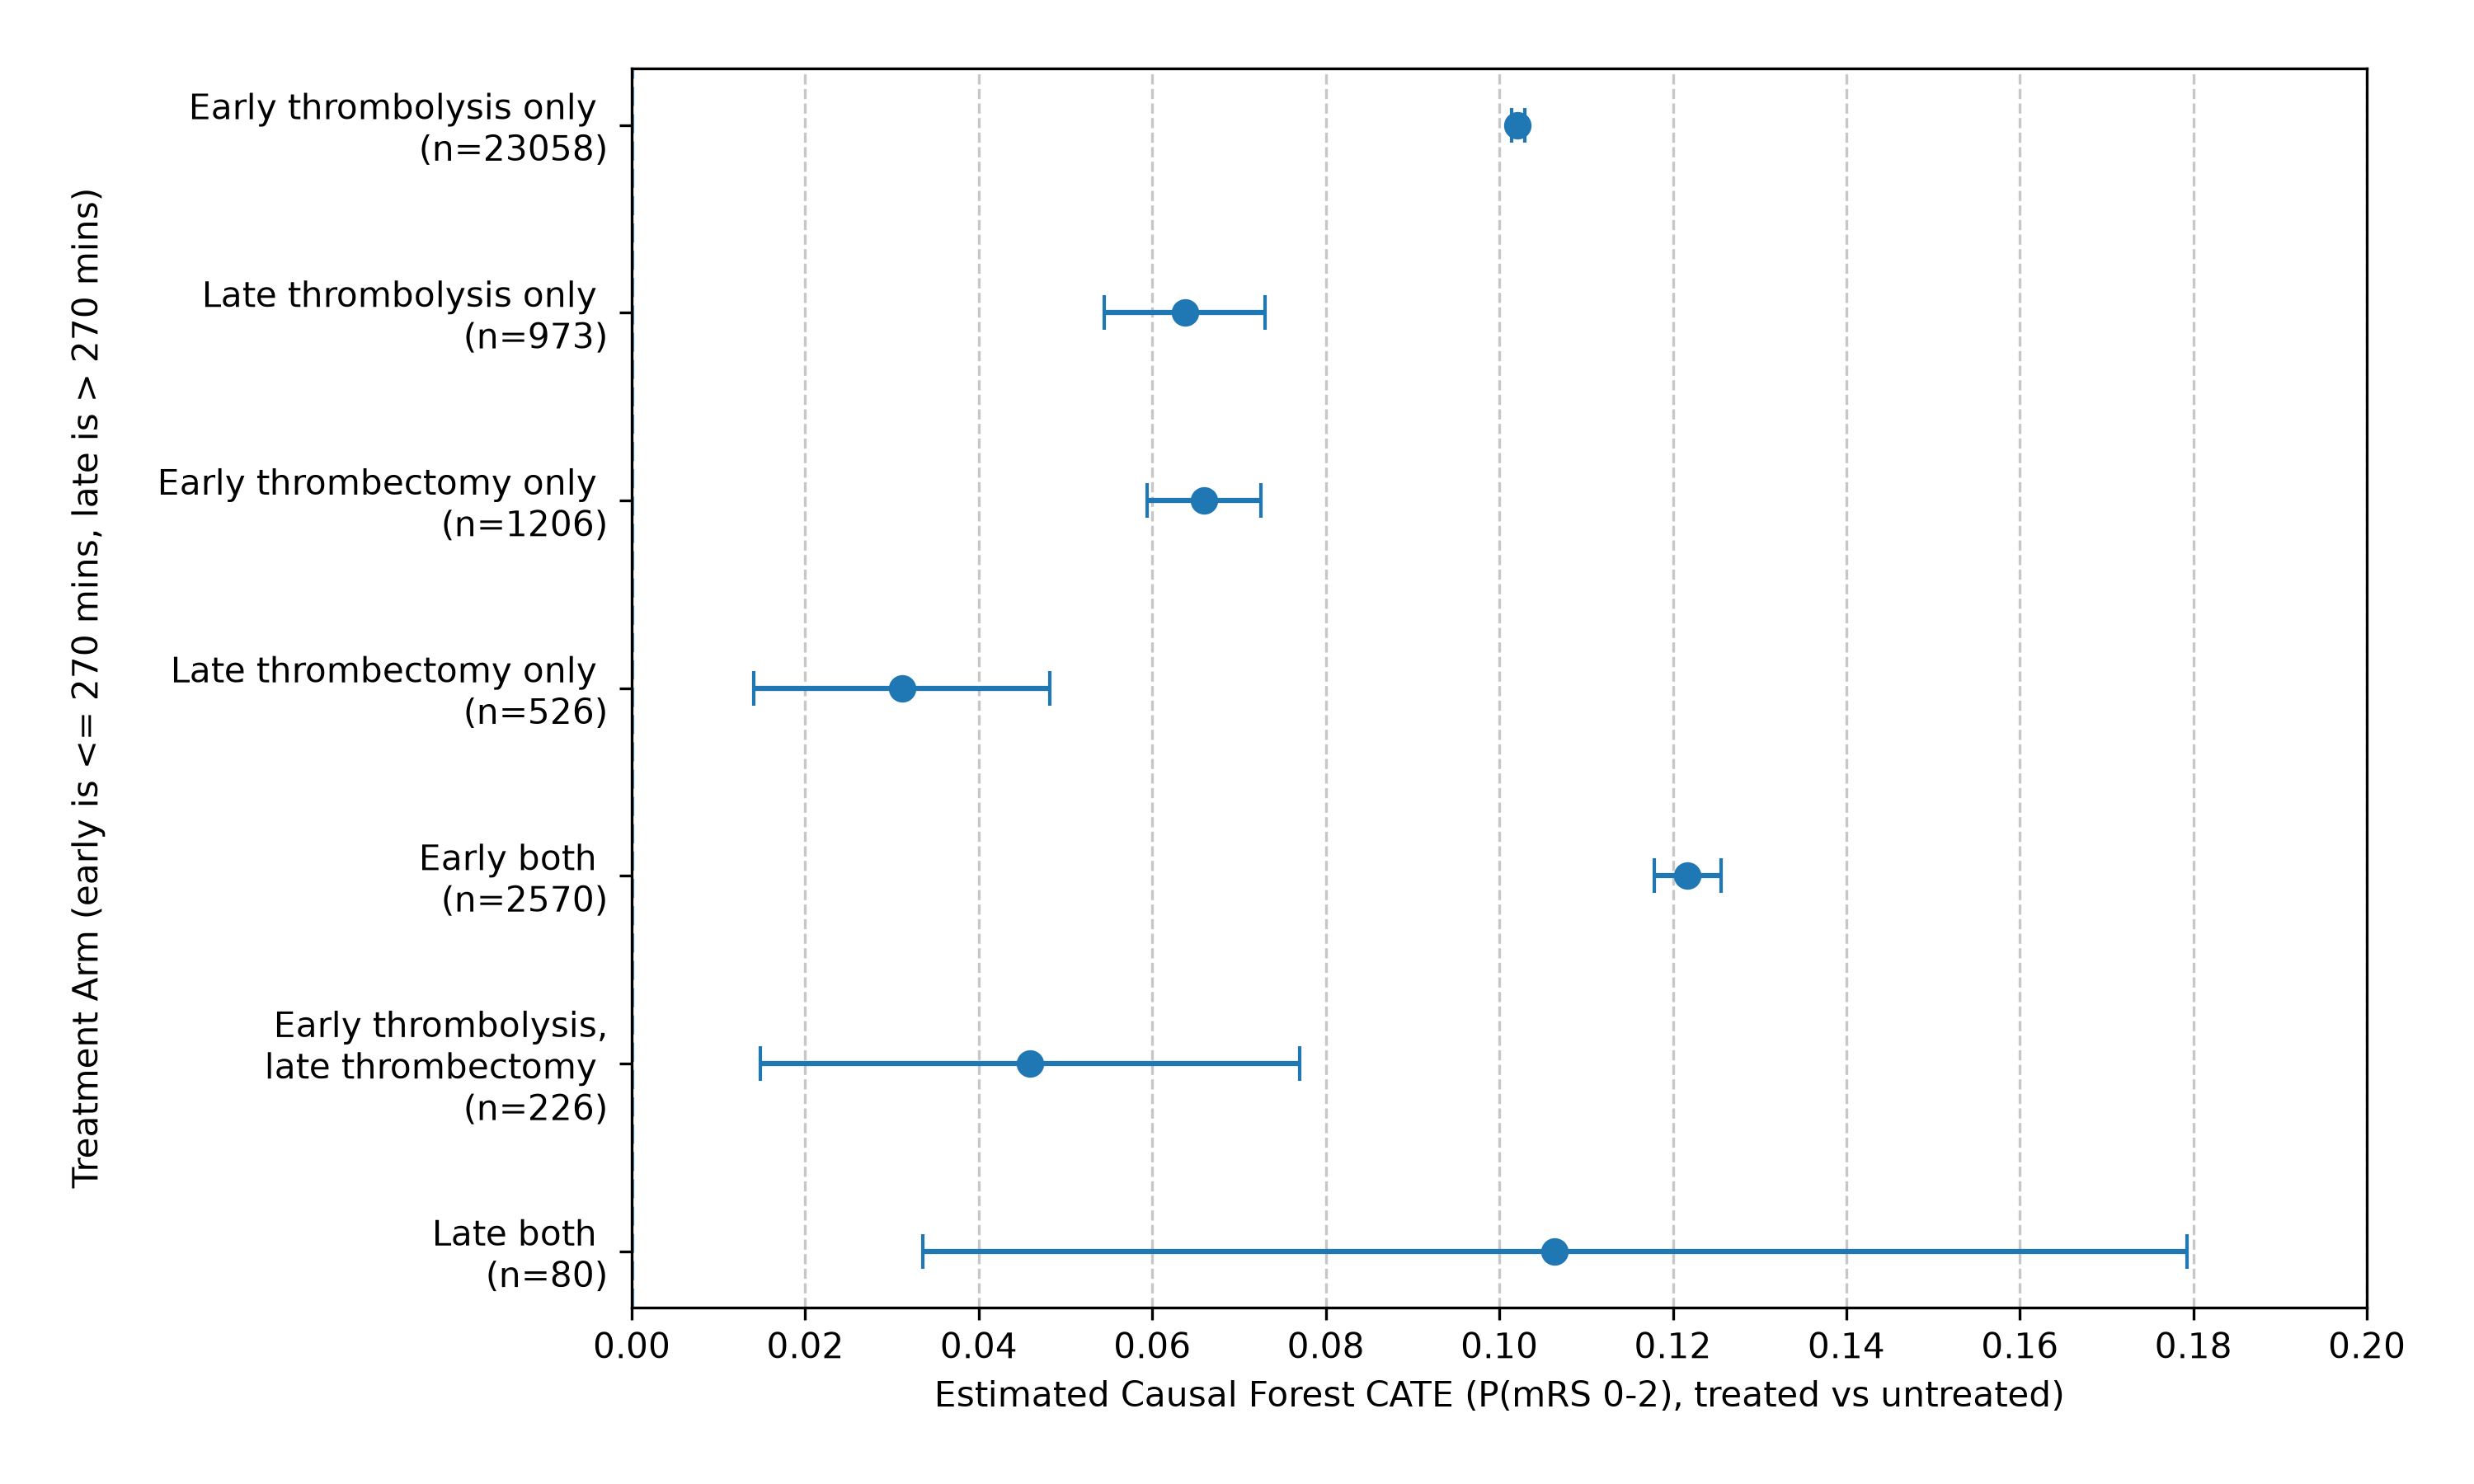
\includegraphics[width=\linewidth]{images/treatment_effects/causal_forest_counterfactual_cate_estimates_2.png}
        %\caption{}
        \label{fig:bottom-left}
    \end{subfigure}

    \vspace{0.5cm} % Optional vertical space between rows

    % Center left image
    \begin{subfigure}{0.49\textwidth}
        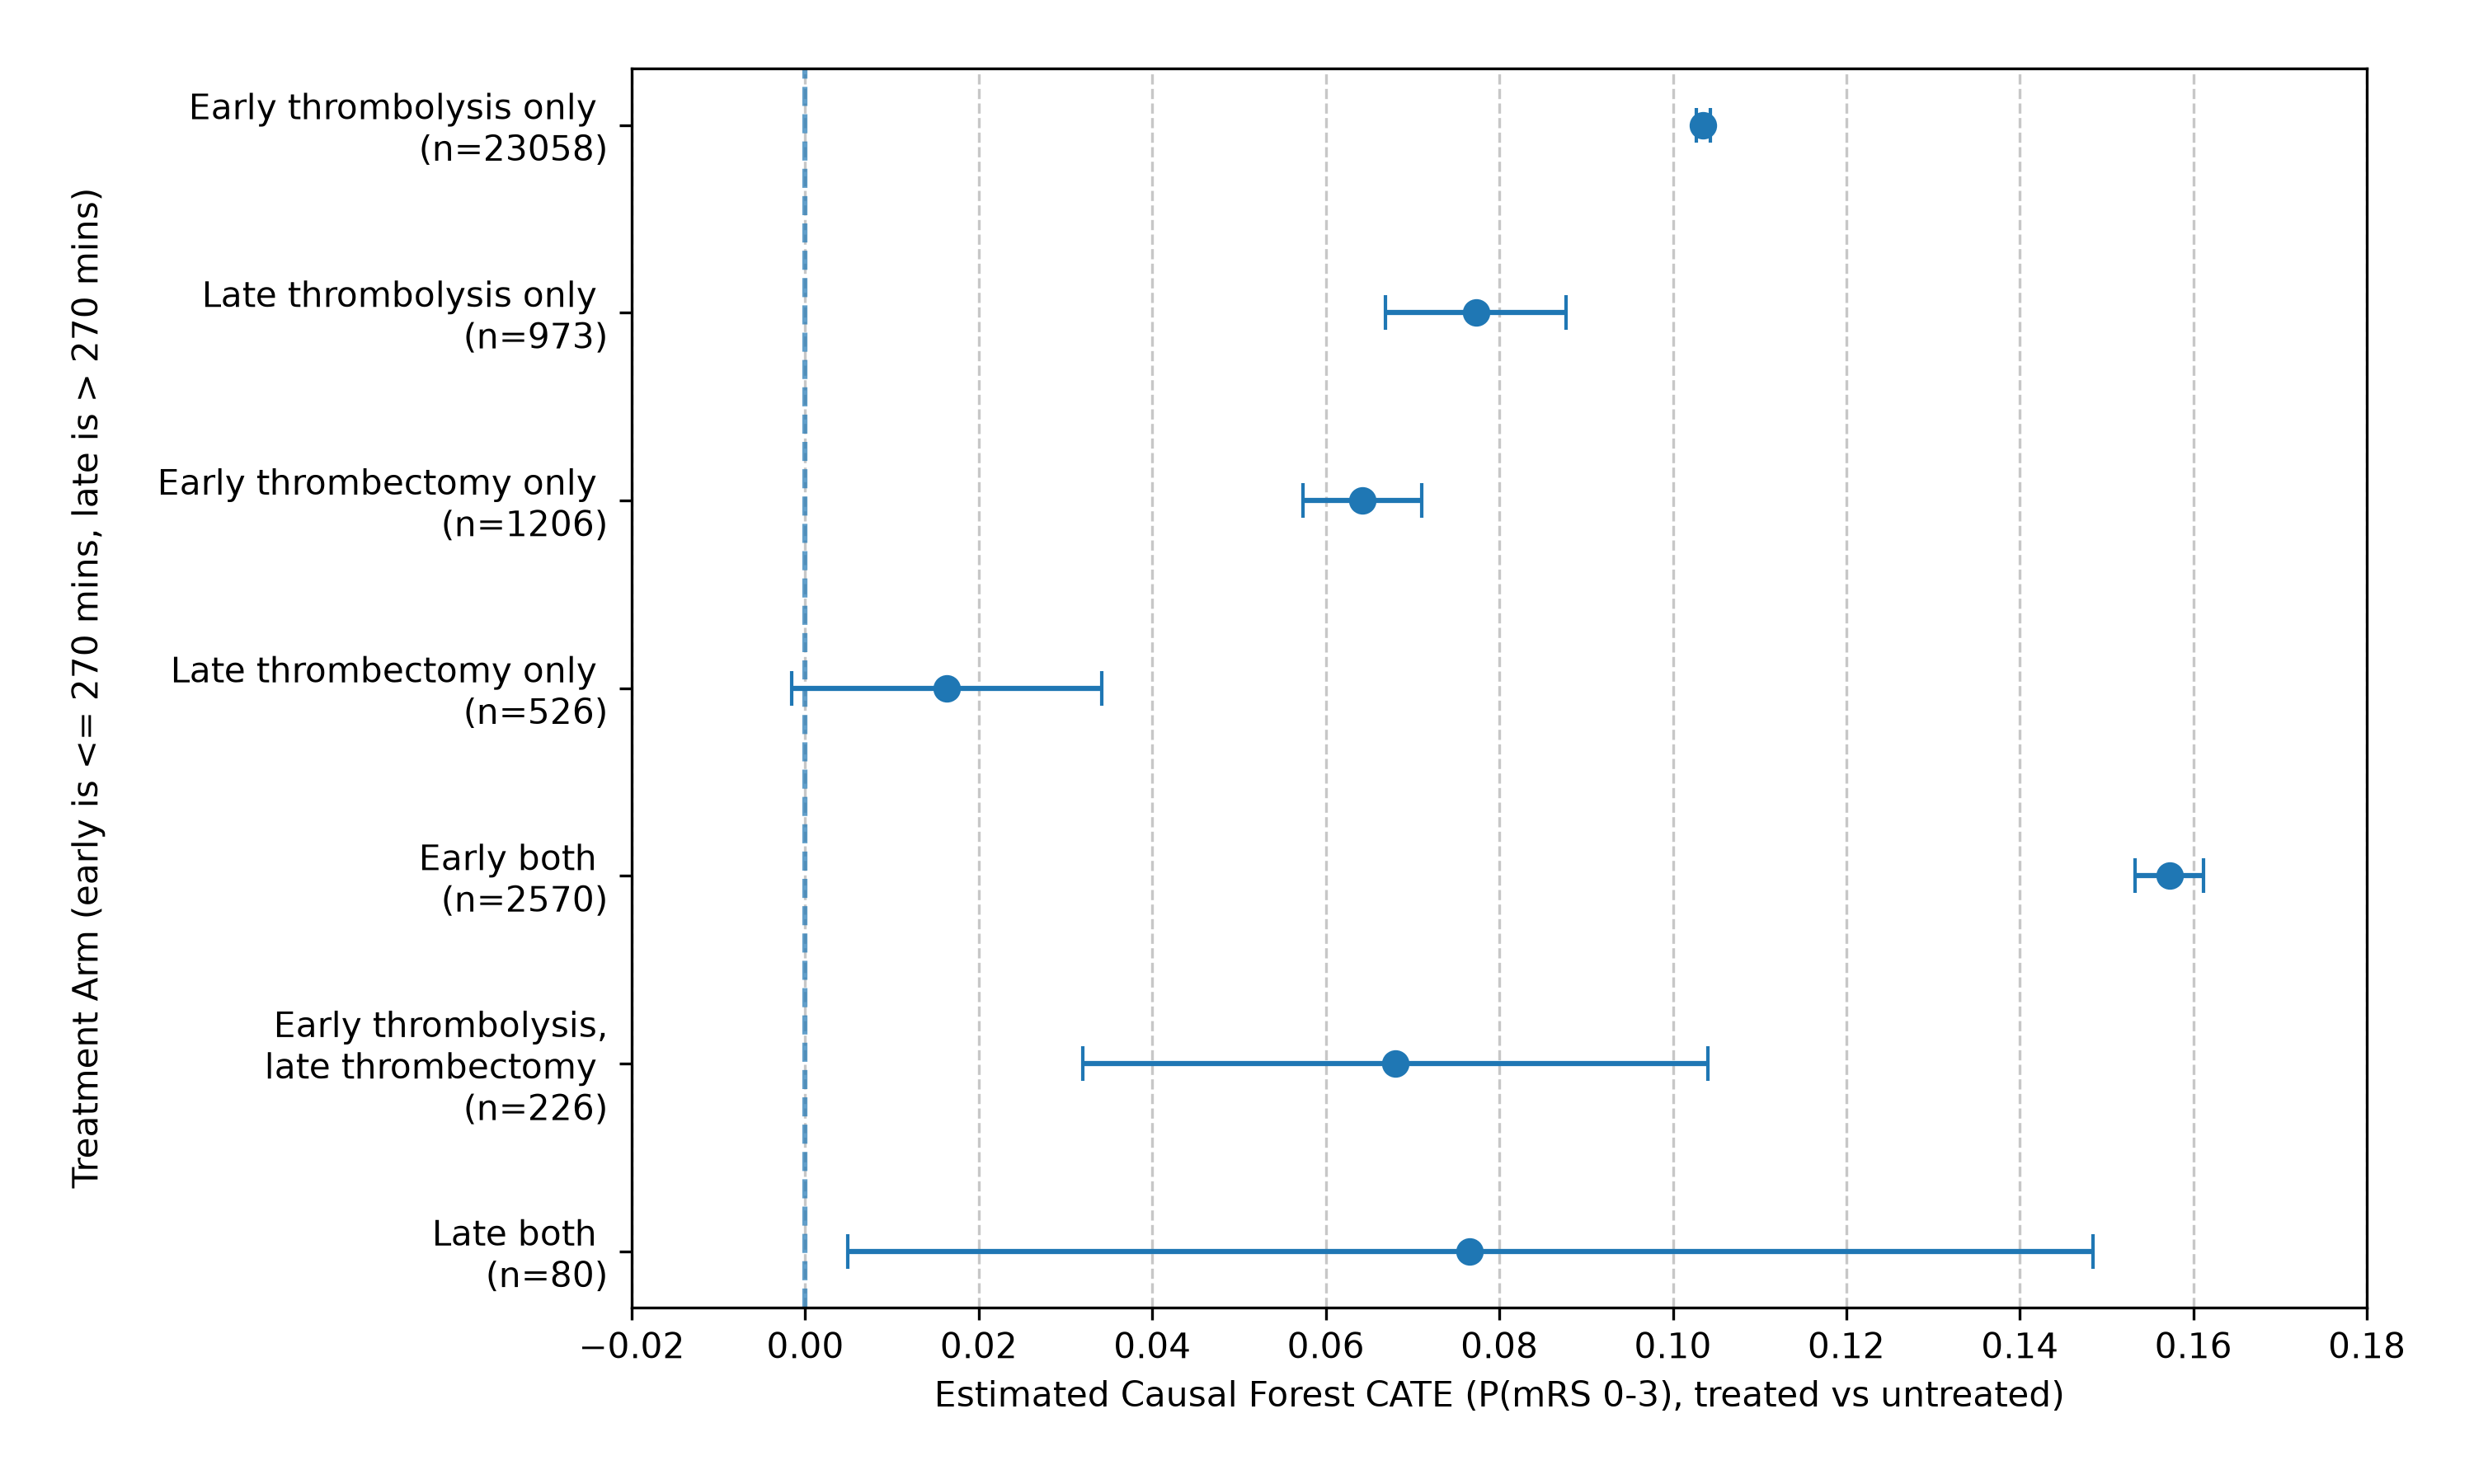
\includegraphics[width=\linewidth]{images/treatment_effects/causal_forest_counterfactual_cate_estimates_3.png}
        %\caption{}
        \label{fig:centre-left}
    \end{subfigure}
    \hfill % Adds flexible horizontal spacing
    % Centre right image 
    \begin{subfigure}{0.49\textwidth}
        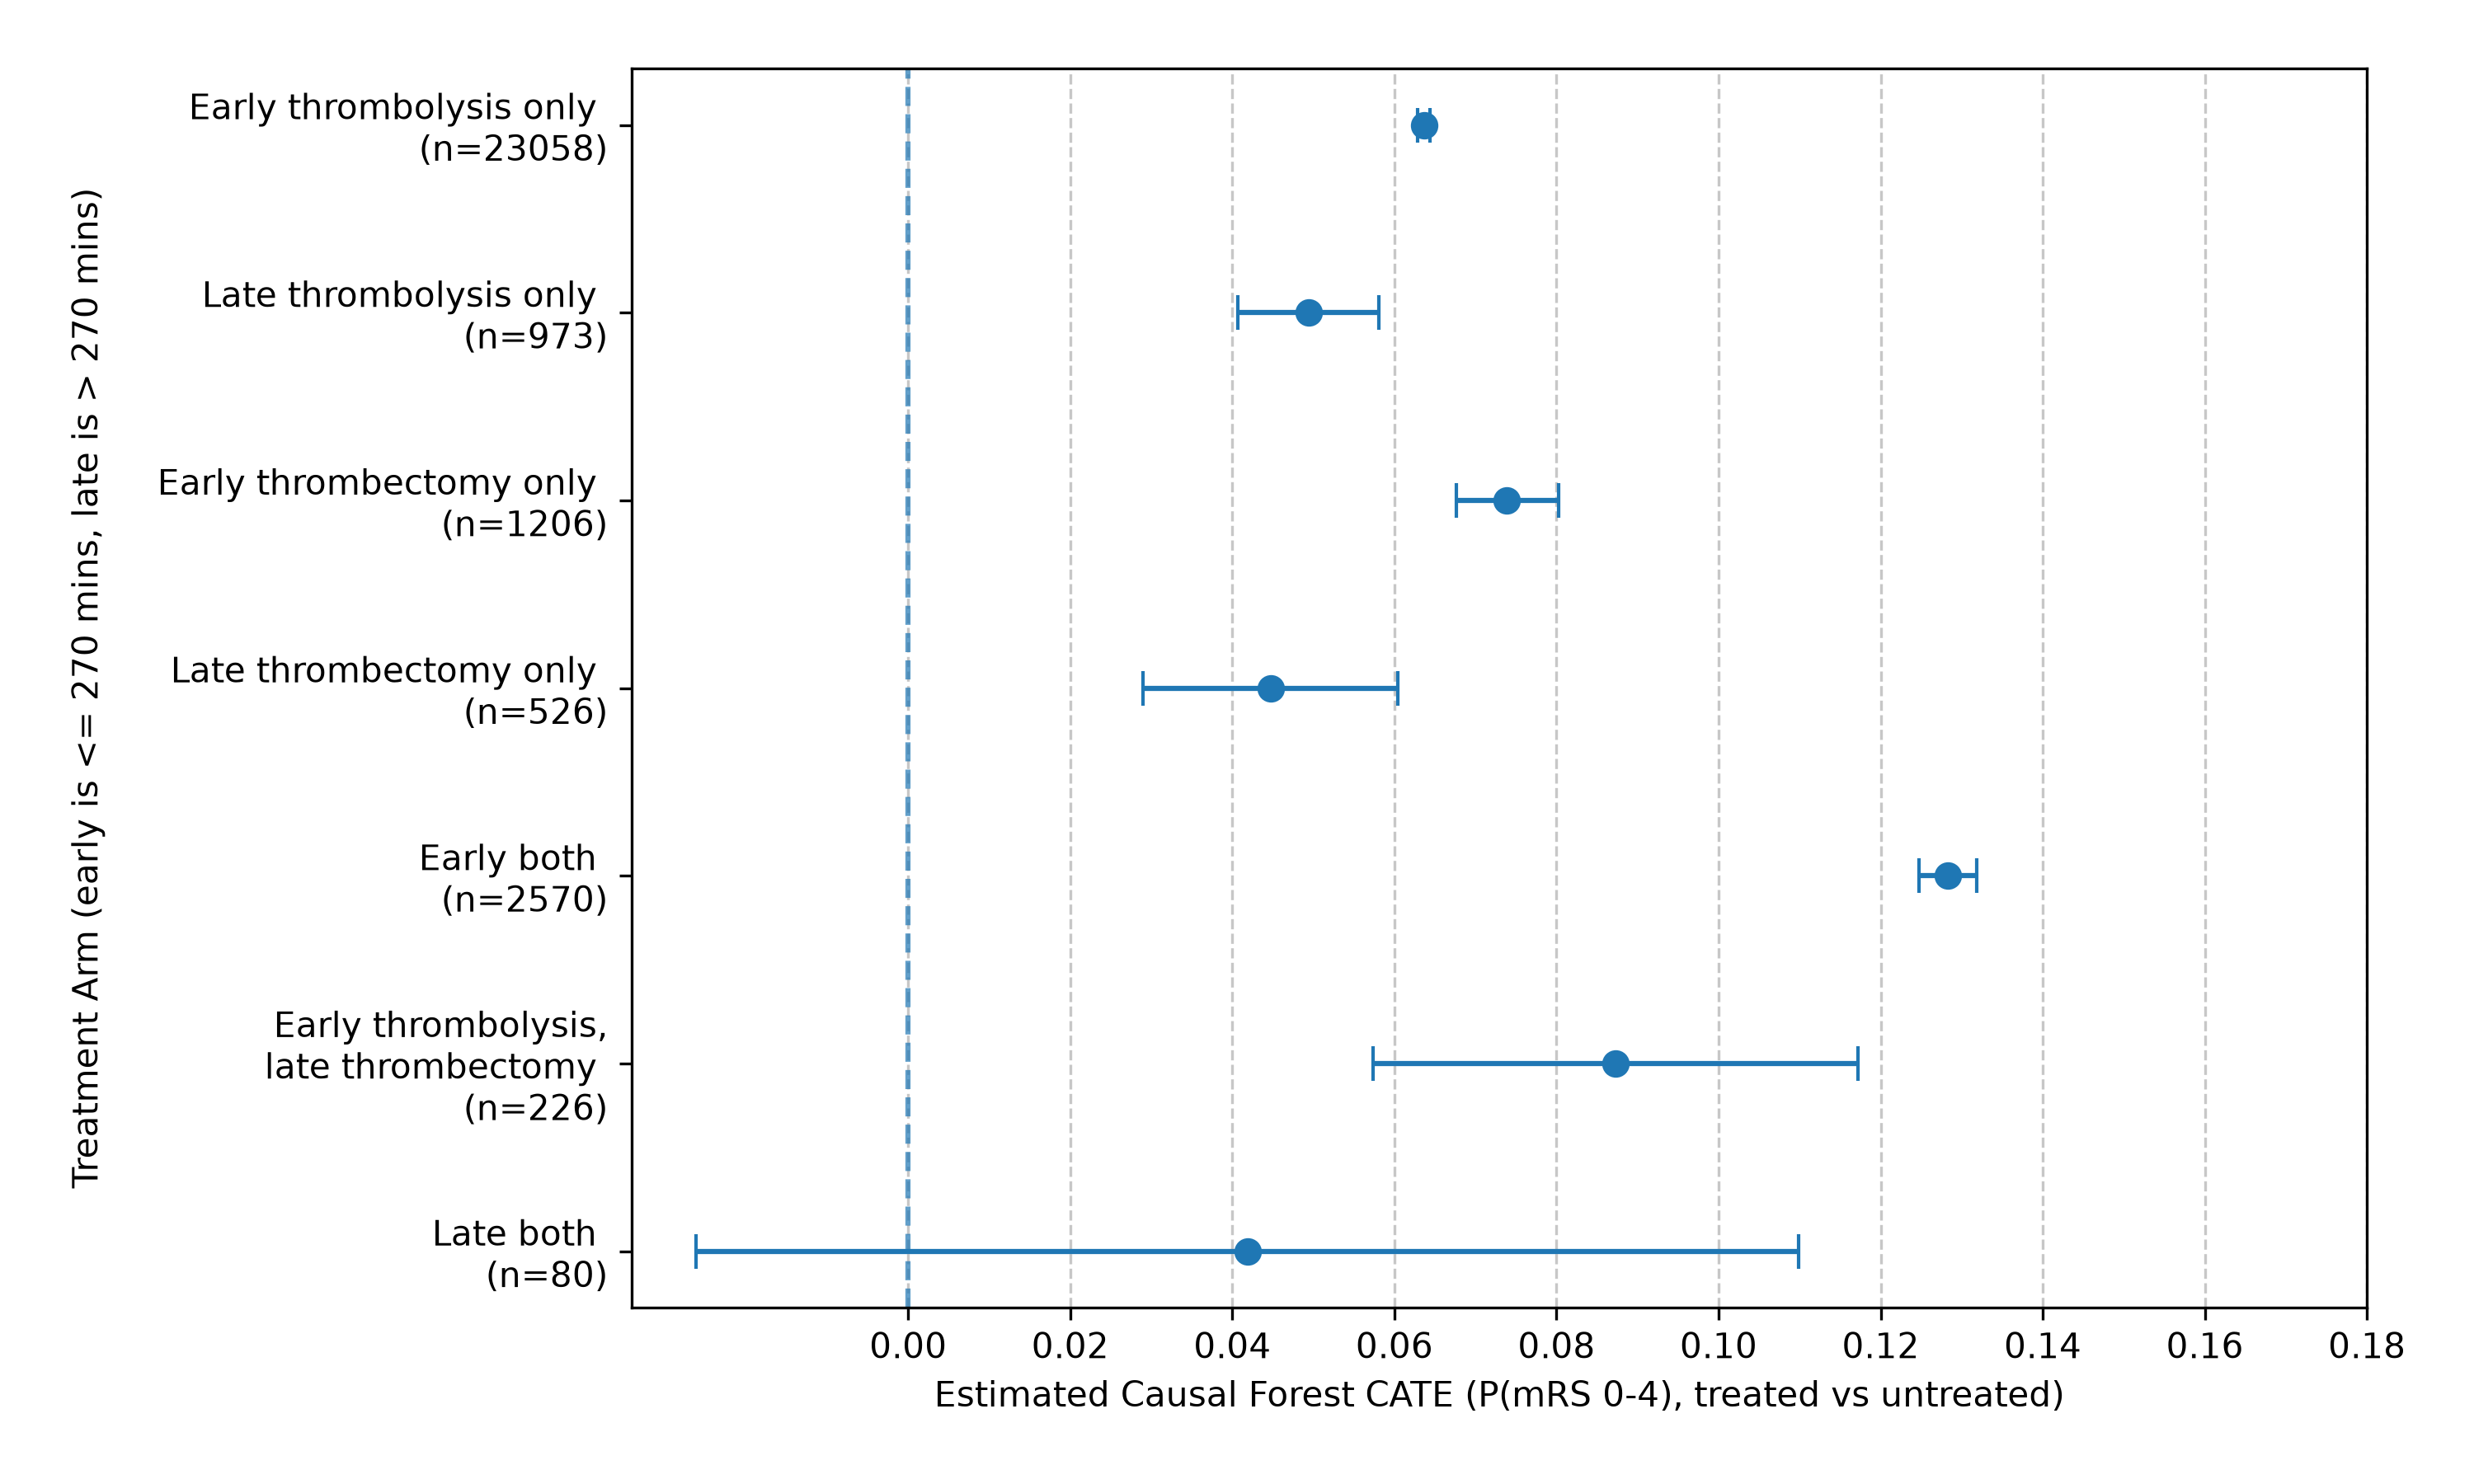
\includegraphics[width=\linewidth]{images/treatment_effects/causal_forest_counterfactual_cate_estimates_4}
        %\caption{}
        \label{fig:centre-right}
    \end{subfigure}

    \vspace{0.5cm} % Optional vertical space between rows

    % Bottom image
    \begin{subfigure}{0.49\textwidth}
        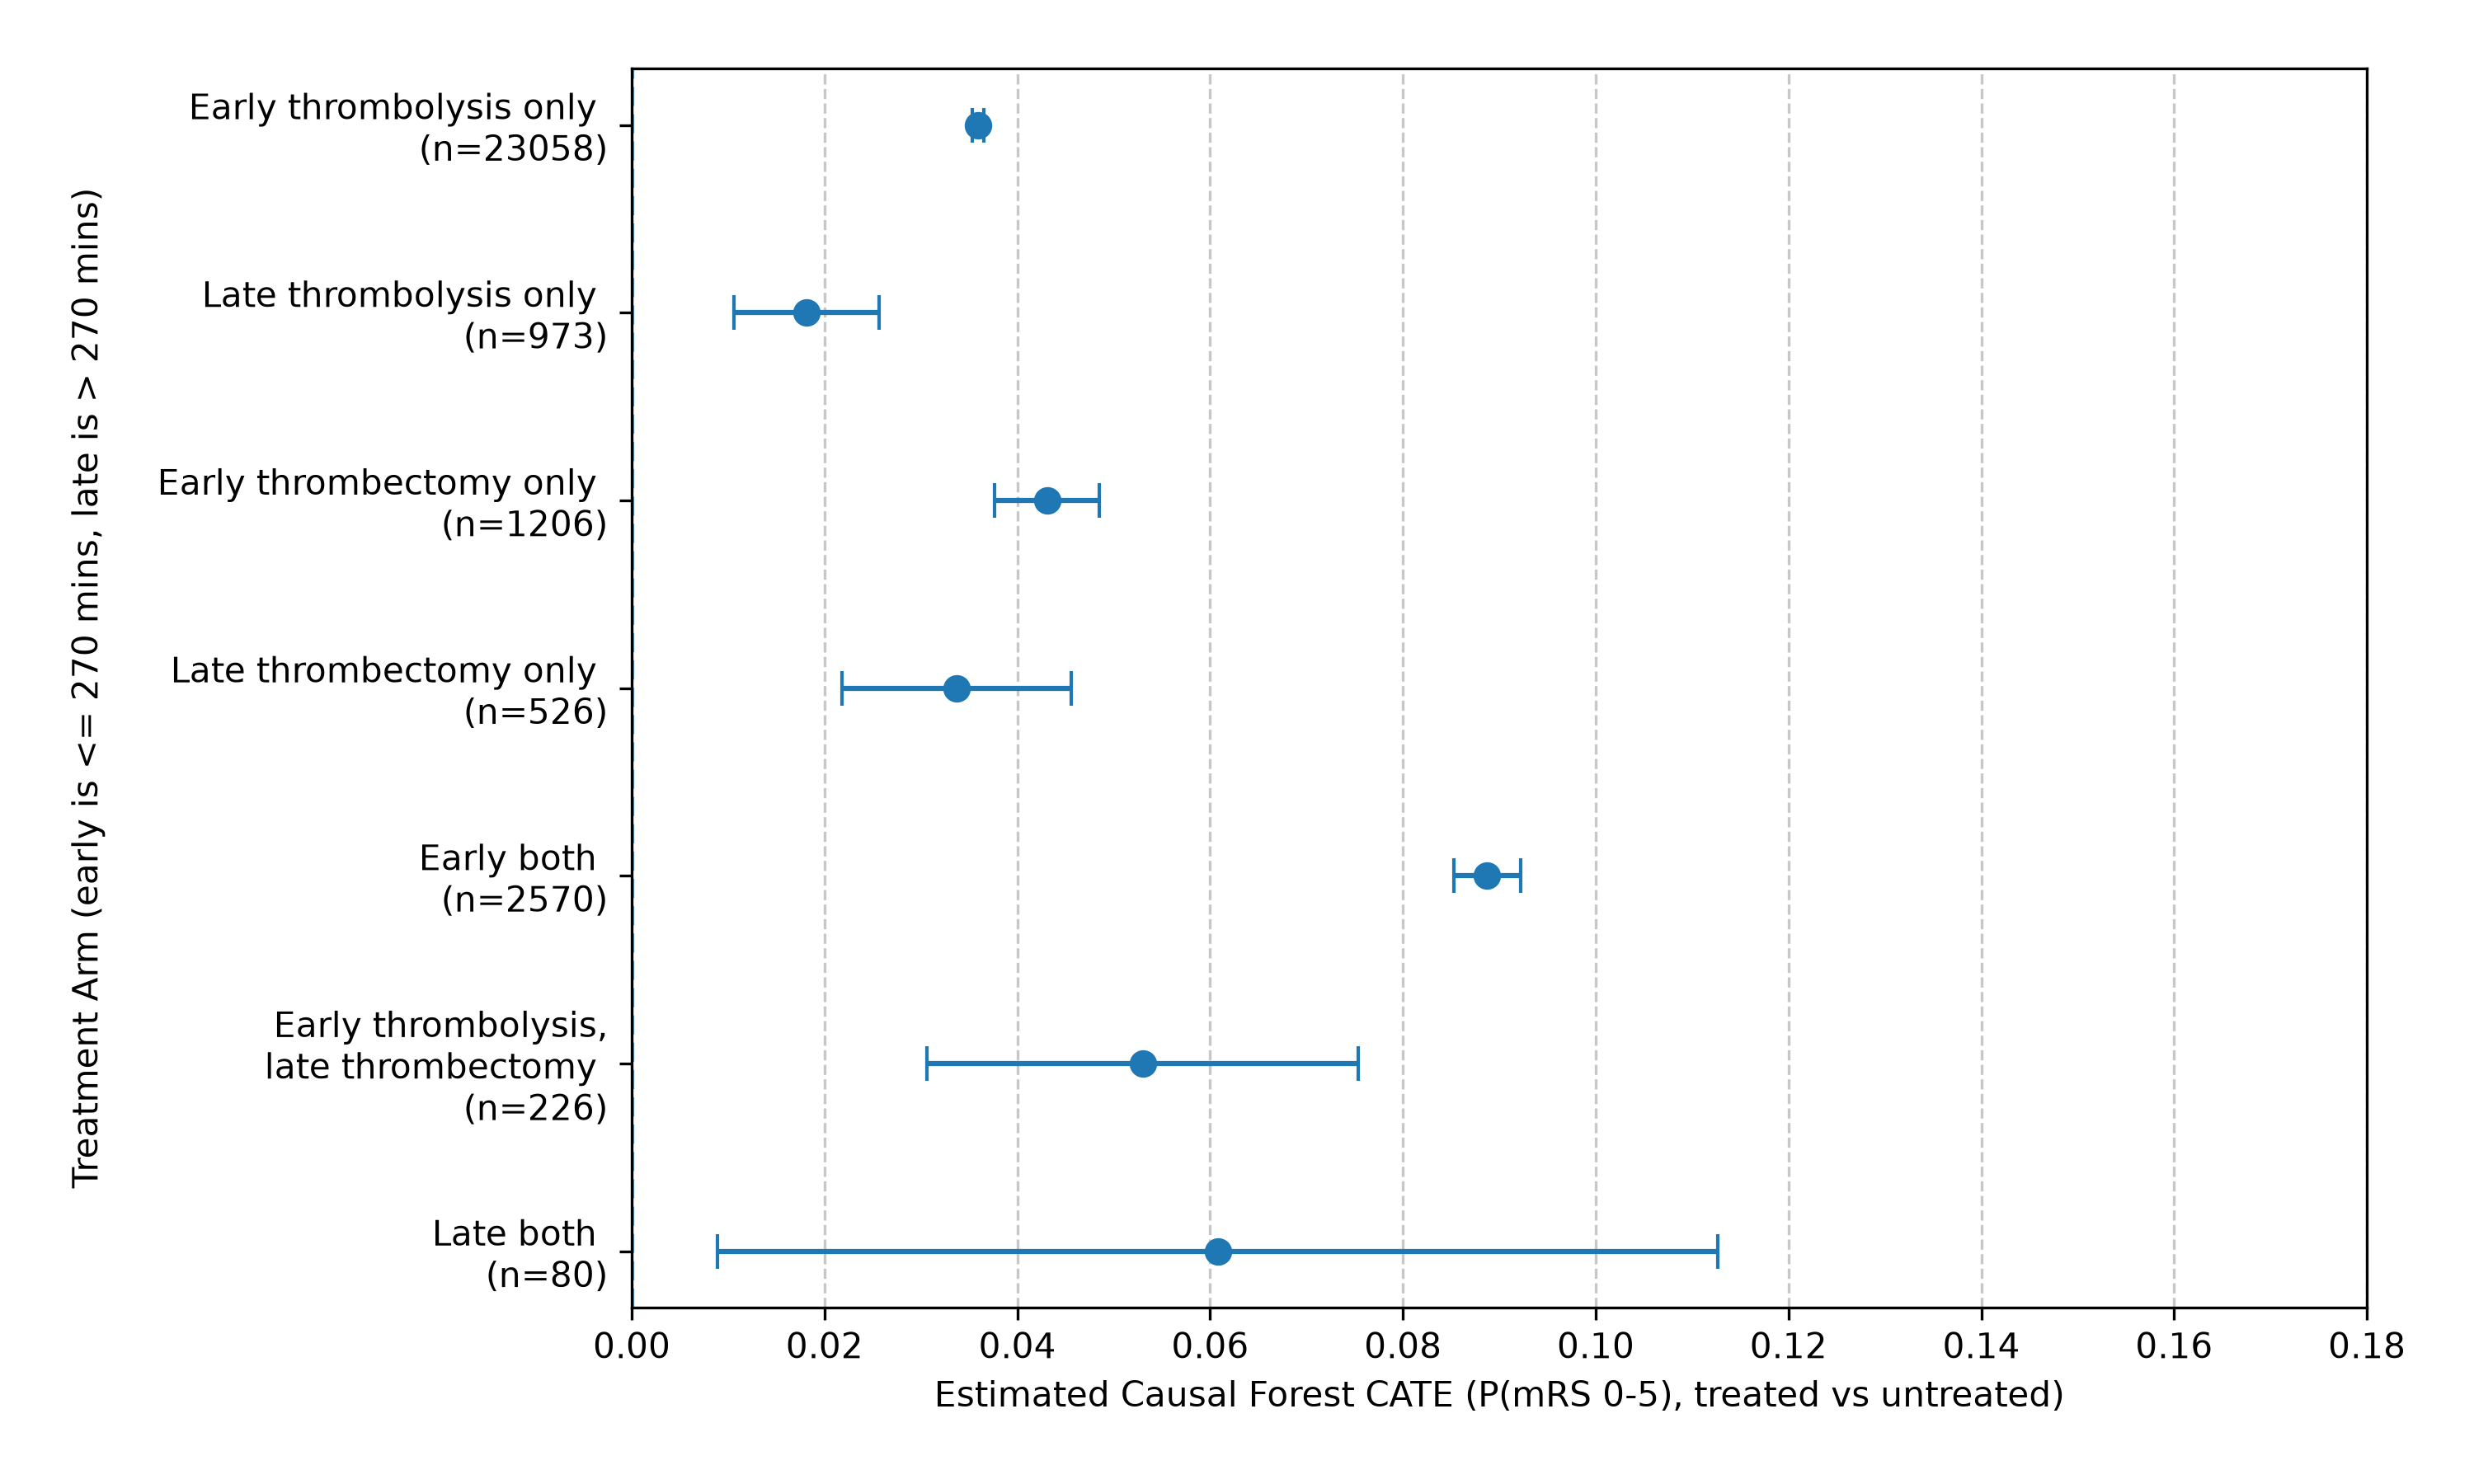
\includegraphics[width=\linewidth]{images/treatment_effects/causal_forest_counterfactual_cate_estimates_5}
        %\caption{}
        \label{fig:centre-right}
    \end{subfigure}
    
    \caption{Estimated counterfactual treatment benefit across reperfusion-treatment timing strategies, derived from the Causal Forest model. Each panel shows results for discharge at or below each modified Rankin Scale (mRS) level. Points represent the mean estimated individual treatment effect for each treatment-timing group, expressed as the counterfactual probability improvement for the specified outcome relative to no reperfusion treatment; horizontal error bars show 95\% confidence intervals. Treatment groups are defined by receipt of intravenous thrombolysis and/or mechanical thrombectomy, with early treatment defined as onset-to-treatment time $<$270 minutes and late treatment as $\geq$270 minutes. Sample sizes are shown alongside group labels. Values above zero indicate a model-predicted increase in the probability of achieving the corresponding mRS outcome under the observed treatment strategy compared with no treatment.}
    \label{fig:causal_forest_benefit}
\end{figure}


